\documentclass[a4paper,11pt]{article}
\pdfoutput=1 % if your are submitting a pdflatex (i.e. if you have
             % images in pdf, png or jpg format)


\usepackage{imakeidx}
\indexsetup{firstpagestyle=empty}
\makeindex[intoc, columns=2, title=Alphabetical Index, options= -s example_style.ist]


\usepackage{jheppub} % for details on the use of the package, please
                     % see the JHEP-author-manual
\usepackage[T1]{fontenc} % if needed

\usepackage{graphicx} % Required for including images
\graphicspath{{Figures/}} % Set the default folder for images

\usepackage{relsize} % for resizing maths relations

\usepackage{enumitem} % Required for manipulating the whitespace between and within lists

\usepackage{subfig} % Required for creating figures with multiple parts (subfigures)

\usepackage{amsmath,amssymb,amsthm,mathrsfs,amsfonts,xfrac,pifont} % For including math equations, theorems, symbols, etc

\usepackage{cleveref} % More descriptive referencing

%page margins and paragraph indentation
%\usepackage{geometry}
%\geometry{a4paper,hmarginratio=1:1}
%\setlength{\parindent}{0pt}

%fonts
  %\usepackage[cm]{sfmath}
  %\renewcommand{\familydefault}{\sfdefault}
  %\usepackage{libertine}
  %\usepackage[libertine]{newtxmath}

\usepackage{array,tabularx}
\usepackage[retainorgcmds]{IEEEtrantools}
\usepackage{etoolbox}
%\usepackage{mathtools}
\usepackage{emerald,xcolor,tikz,pgfplots}
\definecolor{lightergray}{rgb}{0.9,0.9,0.9}






%\usepackage{fixltx2e}
\usepackage{soul}

\usetikzlibrary{matrix,calc,positioning,decorations.markings,decorations.pathmorphing,decorations.pathreplacing}%tikzmark,
\usetikzlibrary{arrows,cd}
\usepackage{bbding}
\usetikzlibrary{positioning}
%\tikzset{every picture/.style={remember picture}}
\tikzset{>=stealth}

\usepackage{cancel}
\newcommand\Ccancel[2][black]{\renewcommand\CancelColor{\color{#1}}\cancel{#2}}

\makeatletter
\patchcmd{\@IEEEeqnarray}{\relax}{\relax\intertext@}{}{}
\makeatother


\usepackage{bm}


%\usepackage[upright]{fourier}
%\newcommand{\tikzmark}[3][]{\tikz[overlay,remember picture,baseline] \node [anchor=base,#1](#2) {#3};}


%\usepackage[cmintegrals,cmbraces]{newtxmath}
%\usepackage{ebgaramond-maths}
%\newcommand{\tikzmark}[1]{\tikz[baseline,remember picture] \coordinate (#1) {};}

%\usepackage{mathptmx}
\usepackage{calc}

%----------------------------------------------------------------------------------------
%	THEOREM STYLES
%---------------------------------------------------------------------------------------

%\newtheoremstyle{dotless}{}{}{\itshape}{}{\bfseries}{}{ }{}
%\theoremstyle{dotless}

\theoremstyle{definition} % Define theorem styles here based on the definition style (used for definitions and examples)
\newtheorem*{definition}{Definition}

\theoremstyle{plain} % Define theorem styles here based on the plain style (used for theorems, lemmas, propositions)
\newtheorem{theorem}{Theorem}[section]
\newtheorem{corollary}[theorem]{Corollary}
\newtheorem{lemma}[theorem]{Lemma}
\newtheorem{proposition}[theorem]{Proposition}

\theoremstyle{remark} % Define theorem styles here based on the remark style (used for remarks and notes)
\newtheorem{example}[theorem]{Example}
\newtheorem*{notation}{Notation}
\newtheorem{remark}[theorem]{Remark}
\newtheorem*{solution}{Solution}


%----------------------------------------------------------------------------------------
%	HYPERLINKS
%---------------------------------------------------------------------------------------
%clever cross-references
%\usepackage[noabbrev,capitalize]{cleveref}

\usepackage{hyperref}
\hypersetup{
%draft, % Uncomment to remove all links (useful for printing in black and white)
colorlinks=true, linkcolor=black, breaklinks=true,
bookmarks=true,bookmarksnumbered=true,
%urlcolor=webbrown, linkcolor=RoyalBlue, citecolor=webgreen, % Link colors
pdftitle={}, % PDF title
pdfauthor={\textcopyright}, % PDF Author
pdfsubject={}, % PDF Subject
pdfkeywords={}, % PDF Keywords
pdfencoding=unicode, %
pdfstartview={FitH}, %
pdfcreator={pdfLaTeX}, % PDF Creator
}

%dotted lines in contents
%\renewcommand{\cftsecleader}{\cftdotfill{\cftdotsep}}



%environment shortcuts 
  \def\ba{\begin{array}}
  \def\ea{\end{array}}
  \def\bc{\begin{corollary}}
  \def\ec{\end{corollary}}
  \def\bd{\begin{definition}}
  \def\ed{\end{definition}}
  \def\ben{\begin{enumerate}}
  \def\een{\end{enumerate}}
  \def\bse{\begin{equation*}}
  \def\ese{\end{equation*}}
  \def\be{\begin{example}}
  \def\ee{\end{example}}
  \def\bi{\begin{IEEEeqnarray*}}
  \def\ei{\end{IEEEeqnarray*}}
  \def\bit{\begin{itemize}}
  \def\eit{\end{itemize}}
  \def\bl{\begin{lemma}}
  \def\el{\end{lemma}}
  \def\bnn{\begin{notation}}
  \def\enn{\end{notation}}
  \def\bn{\begin{note}}
  \def\en{\end{note}}
  \def\bp{\begin{proposition}}
  \def\ep{\end{proposition}}
  \def\bq{\begin{proof}}
  \def\eq{\end{proof}}
  \def\br{\begin{remark}}
  \def\er{\end{remark}}
  \def\bs{\begin{solution}}
  \def\es{\end{solution}}
  \def\btab{\begin{table}}
  \def\etab{\end{table}}
  \def\btb{\begin{tabular}}
  \def\etb{\end{tabular}}
  \def\bt{\begin{theorem}}
  \def\et{\end{theorem}}

%miscellaneous shortcuts
  \def\a{\alpha}
  \def\b{\beta}
  \def\C{\mathbb{C}}
  \def\cA{\mathcal{A}}
  \def\cF{\mathcal{F}}
  \def\cH{\mathcal{H}}
  \def\cJ{\mathcal{J}}
  \def\cK{\mathcal{K}}
  \def\cL{\mathcal{L}}
  \def\cO{\mathcal{O}}
  \def\cP{\mathcal{P}}
  \def\cl{\colon}
  \def\D{\Delta}
  \def\d{\mathrm{d}}
  \def\ds{\displaystyle}
  \def\e{\mathrm{e}}
  \def\eqv{\Leftrightarrow}
  \def\F{\mathbb{F}}
  \def\g{\gamma}
  \def\ic{\mathrm{i}}
  \def\img{\mathrm{im}}
  \def\imp{\Rightarrow}
  \def\iset{\cong_\mathrm{set}}
  \def\l{\lambda}
  \def\la{\langle}
  \def\Mat{\mathrm{Mat}}
  \def\m{\mathrm{m}}
  \def\N{\mathbb{N}}
  \def\n{\nabla}
  \def\ol{\overline}
  \def\p{\partial}
  \def\Q{\mathbb{Q}}
  \def\R{\mathbb{R}}
  \def\ra{\rangle}
  \def\re{\Re\e}
  \def\S{\Sigma}
  \def\s{\sigma}
  \def\se{\subseteq}
  \def\sm{\setminus}
  \def\ss{\subset}
  \def\t{\text}
  \def\ua{\nearrow}
  \def\ve{\varepsilon}
  \def\vn{\varnothing}
  \def\wto{\rightharpoonup}
  \def\Z{\mathbb{Z}}


\def\lacts{\vartriangleright}
\def\racts{\vartriangleleft}
\def\smallblackbox{\mathbin{\raisebox{0.6pt}{\scalebox{0.55}{$\blacksquare$}}}}

\DeclareMathOperator{\Ad}{Ad}
\DeclareMathOperator{\Aut}{Aut}
\DeclareMathOperator{\ad}{ad}
\DeclareMathOperator{\Der}{Der}
\DeclareMathOperator{\End}{End}
\DeclareMathOperator{\ev}{ev}
\DeclareMathOperator{\Gr}{Gr}
\DeclareMathOperator{\Hol}{Hol}
\DeclareMathOperator{\Hom}{Hom}
\DeclareMathOperator{\hor}{hor}
\DeclareMathOperator{\id}{id}
\DeclareMathOperator{\im}{im}
\DeclareMathOperator{\preim}{preim}
\DeclareMathOperator{\proj}{proj}
\DeclareMathOperator{\sgn}{sgn}
\DeclareMathOperator{\lspan}{span}
\DeclareMathOperator{\tr}{tr}
\newcommand{\tvb}[3]{\left(\frac{\partial}{\partial {#1}^{#2}}\right)_{\negmedspace #3}}
\DeclareMathOperator{\ver}{ver}
\DeclareMathOperator{\vol}{vol}




\DeclareMathOperator{\GL}{GL}
\def\gl{\mathfrak{gl}}
\DeclareMathOperator{\Ort}{O}
\def\ort{\mathfrak{o}}
\DeclareMathOperator{\SL}{SL}
\def\sl{\mathfrak{sl}}
\DeclareMathOperator{\SO}{SO}
\def\so{\mathfrak{so}}
\DeclareMathOperator{\SU}{SU}
\def\su{\mathfrak{su}}




\DeclareFontFamily{U}{MnSymbolC}{}
\DeclareSymbolFont{MnSyC}{U}{MnSymbolC}{m}{n}
\DeclareMathSymbol{\diamondplus}{\mathbin}{MnSyC}{"7C}
\DeclareMathSymbol{\diamonddot}{\mathbin}{MnSyC}{"7E}
\DeclareFontShape{U}{MnSymbolC}{m}{n}{
    <-6>  MnSymbolC5
   <6-7>  MnSymbolC6
   <7-8>  MnSymbolC7
   <8-9>  MnSymbolC8
   <9-10> MnSymbolC9
  <10-12> MnSymbolC10
  <12->   MnSymbolC12}{}












\title{\boldmath Lectures on the Geometric Anatomy\\of Theoretical Physics}


%% %simple case: 2 authors, same institution
\author{Dr Frederic P. Schuller} 
%\author{Simon Rea}
\affiliation{Friedrich-Alexander-Universit\"at Erlangen-N\"urnberg,\\Institut f\"ur Theoretische Physik III}

% more complex case: 4 authors, 3 institutions, 2 footnotes
%\author[a,b,1]{F. Irst,\note{Corresponding author.}}
%\author[c]{S. Econd,}
%\author[a,2]{T. Hird\note{Also at Some University.}}
%\author[a,2]{and Fourth}

% The "\note" macro will give a warning: "Ignoring empty anchor..."
% you can safely ignore it.

%\affiliation[a]{One University,\\some-street, Country}
%\affiliation[b]{Another University,\\different-address, Country}
%\affiliation[c]{A School for Advanced Studies,\\some-location, Country}

% e-mail addresses: one for each author, in the same order as the authors
\emailAdd{fps@aei.mpg.de}
%fschuller@perimeterinstitute.ca
%\emailAdd{second@asas.edu}
%\emailAdd{third@one.univ}
%\emailAdd{s.rea.hw@gmail.com}





\begin{document} 

% \rule{0cm}{2cm}\\
% 
\includegraphics[width=14cm]{faulogo}
% \maketitle


% \section*{Introduction}
% \addcontentsline{toc}{section}{Introduction}
% \markright{Introduction}
% Theoretical physics is all about casting our concepts about the real world into rigorous mathematical form, for better or worse. 
But theoretical physical doesn't do that for its own sake.
It does so in order to fully explore the implications of what our concepts about the real world are. So, to a certain extent, the spirit of theoretical physics can be cast into the words of Wittgenstein who said: ``What we cannot speak about [clearly] we must pass over in silence.''
Indeed, if we have concepts about the real world and it is not possible to cast them into rigorous mathematical form, that is usually an indicator that some aspects of these concepts have not been well understood.

Theoretical physical aims at casting these concepts into mathematical language.
But then, mathematics is just that: it is just a language.
If we want to extract physical conclusions from this formulation, we must interpret the language.
That is not the purpose or task of mathematics, that is the task of physicists.
That is where it gets difficult.
But then, again, mathematics is just a language and, going back to Wittgenstein, he said: ``The theorems of mathematics all say the same. Namely, nothing.''
What did he mean by that? Well, obviously, he did not mean that mathematics is useless.
He just referred to the fact that if we have a theorem of the type ``$A$ if, and only if, $B$'', where $A$ and $B$ are propositions, then obviously $B$ says nothing else that $A$ does, and $A$ says nothing else than $B$ does.
It is a tautology. However, while from the point of view of logic and mathematics it is a tautology, psychologically, in terms of our understanding of $A$, it may be very useful to have a reformulation of $A$ in terms of $B$.

Thus, with the understanding that mathematics just gives us a language for what we want to do, the idea of this course is to provide proper language for theoretical physics. In particular, we will provide the proper mathematical language for classical mechanics, electromagnetism, quantum mechanics and statistical physics. We are not going to revise all the mathematics that is needed for these four subjects, but rather we will develop the mathematics from a higher point of view assuming some prior knowledge of these subjects.





























% \newpage

% \section{Logic of propositions and predicates}
% \subsection{Propositional logic}

\bd
A \emph{proposition}\index{proposition} $p$ is a variable\footnote{By this we mean a formal expression, with no extra structure assumed.} that can take the values \emph{true} ($T$) or \emph{false} ($F$), and no others.
\ed

This is what a proposition is from the point of view of propositional logic.
In particular, it is not the task of propositional logic to decide whether a complex statement of the form ``there is extraterrestrial life'' is true or not.
Propositional logic already deals with the complete proposition, and it just assumes that is either true or false.
It is also not the task of propositional logic to decide whether a statement of the type ``in winter is colder than outside'' is a proposition or not (i.e. if it has the property of being either true or false).
In this particular case, the statement looks rather meaningless.

\bd
A proposition which is always true is called a \emph{tautology}\index{tautology}, while one which is always false is called a \emph{contradiction}\index{contradiction}.
\ed

It is possible to build new propositions from given ones using \emph{logical operators}.
The simplest kind of logical operators are \emph{unary} operators, which take in one proposition and return another proposition.
There are four unary operators in total, and they differ by the truth value of the resulting proposition which, in general, depends on the truth value of $p$.
We can represent them in a table as follows:

\btab[h!]
\centering
\btb{c||c|c|c|c}
$p$ & $\neg p$ & $\mathrm{id}(p)$ & $\top p$ & $\bot p$ \\
\hline
\rule{0pt}{12pt} F & T & F & T & F\\
T & F & T & T & F
\etb
\etab
where $\neg$ is the \emph{negation} operator, $\mathrm{id}$ is the \emph{identity} operator, $\top$ is the \emph{tautology} operator and $\bot$ is the \emph{contradiction} operator.
These clearly exhaust all possibilities for unary operators.

The next step is to consider \emph{binary} operators, i.e. operators that take in two propositions and return a new proposition.
There are four combinations of the truth values of two propositions and, since a binary operator assigns one of the two possible truth values to each of those, we have 16 binary operators in total.
The operators $\land$, $\lor$ and~$\veebar$, called \emph{and}, \emph{or} and \emph{exclusive or} respectively, should already be familiar to you.

\btab[h!]
\centering
\btb{c|c||c|c|c}
$p$ & $q$ & $p\land q$ & $p\lor q$ & $p\veebar q$ \\
\hline
\rule{0pt}{12pt} F & F & F & F & F\\
F & T & F & T & T\\
T & F & F & T & T\\
T & T & T & T & F
\etb
\etab

There is one binary operator, the \emph{implication}\index{implication} operator $\imp$, which is sometimes a little ill understood, unless you are already very knowledgeable about these things. Its usefulness comes in conjunction with the \emph{equivalence} operator $\eqv$. We have:

\btab[h!]
\centering
\btb{c|c||c|c}
$p$ & $q$ & $p\imp q$ & $p\eqv q$ \\
\hline
\rule{0pt}{12pt} F & F & T & T \\
F & T & T & F \\
T & F & F & F \\
T & T & T & T 
\etb
\etab

While the fact that the proposition $p\imp q$ is true whenever $p$ is false may be surprising at first, it is just the definition of the implication operator and it is an expression of the principle ``Ex falso quod libet'', that is, from a false assumption anything follows.
Of course, you may be wondering why on earth we would want to define the implication operator in this way.
The answer to this is hidden in the following result.

\bt
Let $p,q$ be propositions.
Then $(p\imp q) \eqv ((\neg q)\imp (\neg p))$.
\et

\bq
We simply construct the truth tables for $p\imp q$ and $ (\neg q)\imp (\neg p)$.

\btab[h!]
\centering
\btb{c|c||c|c|c|c}
$p$ & $q$ & $\neg p$ & $\neg q$ & $p\imp q$ & $(\neg q)\imp (\neg p)$ \\
\hline
\rule{0pt}{12pt} F & F & T & T & T & T\\
F & T & T & F & T & T\\
T & F & F & T & F & F\\
T & T & F & F & T & T
\etb
\etab

The columns for $p\imp q$ and $ (\neg q)\imp (\neg p)$ are identical and hence we are done.
\eq

\br
We agree on decreasing binding strength in the sequence:
\bse
\neg \, , \ \land \, , \ \lor \, , \ \imp \, , \ \eqv .
\ese
For example, $(\neg q)\imp (\neg p)$ may be written unambiguously as $\neg q\imp \neg p$.
\er

\br
All higher order operators $\heartsuit (p_1,\ldots,p_N)$ can be constructed from a single binary operator defined by:

\btab[h!]
\centering
\btb{c|c||c}
$p$ & $q$ & $ p \uparrow q$ \\
\hline
\rule{0pt}{12pt} F & F & T \\
F & T & T \\
T & F & T\\
T & T & F
\etb
\etab

This is called the \emph{nand} operator and, in fact, we have $(p \uparrow q) \eqv \neg (p \land q)$.
\er

\subsection{Predicate logic}

\bd
A \emph{predicate}\index{predicate} is (informally) a proposition-valued function of some variable or variables. In particular, a predicate of two variables is called a \emph{relation}\index{relation}.
\ed

For example, $P(x)$ is a proposition for each choice of the variable $x$, and its truth value depends on $x$.
Similarly, the predicate $Q(x,y)$ is, for any choice of $x$ and $y$, a proposition and its truth value depends on $x$ and $y$.

Just like for propositional logic, it is not the task of predicate logic to examine how predicates are built from the variables on which they depend.
In order to do that, one would need some further language establishing the rules to combine the variables $x$ and $y$ into a predicate.
Also, you may want to specify from which ``set'' $x$ and $y$ come from.
Instead, we leave it completely open, and simply consider $x$ and $y$ formal variables, with no extra conditions imposed.

This may seem a bit weird since from elementary school one is conditioned to always ask where "x" comes from upon seeing an expression like $P(x)$.
However, it is crucial that we refrain from doing this here, since we want to only later define the notion of set, using the language of propositional and predicate logic.
As with propositions, we can construct new predicates from given ones by using the operators define in the previous section. For example, we might have:
\bse
Q(x,y,z) :\eqv P(x) \land R(y,z),
\ese
where the symbol $:\eqv$ means ``defined as being equivalent to''.
More interestingly, we can construct a new proposition from a given predicate by using \emph{quantifiers}.
\bd
Let $P(x)$ be a predicate. Then:
\bse
\forall \, x : P(x) ,
\ese
is a proposition, which we read as ``for all $x$, $P$ of $x$ (is true)'', and it is defined to be true if $P(x)$ is true independently of $x$, false otherwise. The symbol $\forall$\index{$\forall$} is called \emph{universal quantifier}\index{universal quantifier}.
\ed
\bd
Let $P(x)$ be a predicate.
Then we define:
\bse
\exists \, x : P(x) : \eqv \neg (\forall \, x : \neg P(x)).
\ese
The proposition $\exists \, x : P(x)$ is read as ``there exists (at least one) $x$ such that $P$ of $x$ (is true)'' and the symbol $\exists$\index{$\exists$} is called \emph{existential quantifier}\index{existential quantifier}.
\ed
The following result is an immediate consequence of these definitions.
\bc
Let $P(x)$ be a predicate. Then:
\bse
\forall \, x : P(x) \eqv \neg (\exists \, x : \neg P(x) ).
\ese
\ec
\br
It is possible to define quantification of predicates of more than one variable.
In order to do so, one proceeds in steps quantifying a predicate of one variable at each step. 
\er
\be
Let $P(x,y)$ be a predicate.
Then, for fixed $y$, $P(x,y)$ is a predicate of one variable and we define:
\bse
Q(y) :\eqv \forall \, x : P(x,y).
\ese
Hence we may have the following:
\bse
\exists \, y : \forall \, x : P(x,y) :\eqv \exists \, y : Q(y).
\ese
Other combinations of quantifiers are defined analogously.
\ee
\br
The order of quantification matters (if the quantifiers are not all the same).
For a given predicate $P(x,y)$, the propositions:
\bse
\exists \, y : \forall \, x : P(x,y)  \quad \text{and} \quad \forall \, x : \exists \, y : P(x,y) 
\ese
are not necessarily equivalent.
\er
\be
Consider the proposition expressing the existence of additive inverses in the real numbers. We have:
\bse
\forall \, x : \exists \, y : \ x+y=0,
\ese
i.e. for each $x$ there exists an inverse $y$ such that $x+y=0$. For $1$ this is $-1$, for $2$ it is $-2$ etc.
Consider now the proposition obtained by swapping the quantifiers in the previous proposition:
\bse
\exists \, y : \forall \, x : \ x+y=0.
\ese

What this proposition is saying is that there exists a real number $y$ such that, no matter what $x$ is, we have $x+y=0$.
This is clearly false, since if $x+y=0$ for some $x$ then $(x+1)+y\neq 0$, so the same $y$ cannot work for both $x$ and $x+1$, let alone every $x$.
\ee
Notice that the proposition $\exists \, x : P(x)$ means ``there exists \emph{at least one} $x$ such that $P(x)$ is true''. Often in mathematics we prove that ``there exists \emph{a unique} $x$ such that $P(x)$ is true''. We therefore have the following definition.

\bd
Let $P(x)$ be a predicate. We define the \emph{unique existential quantifier} $\exists !$ by:
\bse
\exists ! \, x : P(x) :\eqv (\exists \, x : P(x)) \land \forall \, y : \forall \, z : (P(y)\land P(z) \imp y=z) .
\ese
\ed
This definition clearly separates the existence condition from the uniqueness condition. An equivalent definition with the advantage of brevity is:
\bse
\exists ! \, x : P(x) :\eqv (\exists \, x : \forall \, y : P(y) \eqv x=y)
\ese

\subsection{Axiomatic systems and theory of proofs}

\bd
An \emph{axiomatic system} is a finite sequence of propositions $a_1,a_2,\ldots,a_N$, which are called the \emph{axioms}\index{axiom} of the system.
\ed

\bd
A \emph{proof}\index{proof} of a proposition $p$ within an axiomatic system $a_1,a_2,\ldots,a_N$ is a finite sequence of propositions $q_1,q_2,\ldots,q_M$ such that $q_M=p$ and for any $1\leq j \leq M$ one of the following is satisfied:
\ben
\item[(A)] $q_j$ is a proposition from the list of axioms;
\item[(T)] $q_j$ is a tautology;
\item[(M)] $\exists \, 1\leq m,n <j : (q_m\land q_n \imp q_j)$ is true.
\een
\ed
\br
If $p$ can be proven within an axiomatic system $a_1,a_2,\ldots,a_N$, we write:
\bse
a_1,a_2,\ldots,a_N \vdash p
\ese
and we read ``$a_1,a_2,\ldots,a_N$ proves $p$''.
\er
\br
This definition of proof allows to easily recognise a proof.
A computer could easily check that whether or not the conditions (A), (T) and (M) are satisfied by a sequence of propositions.
To actually find a proof of a proposition is a whole different story.
\er
\br
Obviously, any tautology that appears in the list of axioms of an axiomatic system can be removed from the list without impairing the power of the axiomatic system.  
\er

An extreme case of an axiomatic system is propositional logic.
The axiomatic system for propositional logic is the empty sequence.
This means that all we can prove in propositional logic are tautologies.

\bd
An axiomatic system $a_1,a_2,\ldots,a_N$ is said to be \emph{consistent}\index{consistency} if there exists a proposition $q$ which cannot be proven from the axioms.
In symbols:
\bse
\exists \, q : \neg (a_1,a_2,\ldots,a_N \vdash q).
\ese
\ed

The idea behind this definition is the following.
Consider an axiomatic system which contains contradicting propositions:
\bse
a_1,\ldots,s,\ldots,\neg s,\ldots,a_N .
\ese
Then, given \emph{any} proposition $q$, the following is a proof of $q$ within this system:
\bse
s, \neg s, q.
\ese
Indeed, $s$ and $\neg s$ are legitimate steps in the proof since they are axioms.
Moreover, $s\land \neg s$ is a contradiction and thus $(s\land \neg s) \imp q$ is a tautology.
Therefore, $q$ follows from condition (M).
This shows that any proposition can be proven within a system with contradictory axioms.
In other words, the inability to prove every proposition is a property possessed by no contradictory system, and hence we define a consistent system as one with this property.

Having come this far, we can now state (and prove) an impressively sounding theorem.

\bt
Propositional logic is consistent.
\et

\bq
Suffices to show that there exists a proposition that cannot be proven within propositional logic. Propositional logic has the empty sequence as axioms.
Therefore, only conditions (T) and (M) are relevant here.
The latter allows the insertion of a proposition $q_j$ such that $(q_m\land q_n) \imp q_j$ is true, where $q_m$ and $q_n$ are propositions that precede $q_j$ in the proof sequence.
However, since (T) only allows the insertion of a tautology anywhere in the proof sequence, the propositions $q_m$ and $q_n$ must be tautologies.
Consequently, for $(q_m\land q_n) \imp q_j$ to be true, $q_j$ must also be a tautology.
Hence, the proof sequence consists entirely of tautologies and thus only tautologies can be proven.

Now let $q$ be any proposition.
Then $q\land \neg q$ is a contradiction, hence not a tautology and thus cannot be proven.
Therefore, propositional logic is consistent.
\eq

\br
While it is perfectly fine and clear how to define consistency, it is perfectly difficult to prove consistency for a given axiomatic system, propositional logic being a big exception.
\er

\bt
Any axiomatic system powerful enough to encode elementary arithmetic is either inconsistent or contains an \emph{undecidable}\index{undecidable} proposition, i.e.\ a proposition that can be neither proven nor disproven within the system.
\et

An example of an undecidable proposition is the Continuum hypothesis within the Zermelo-Fraenkel axiomatic system.  





















% \newpage

% \section{Axioms of set theory}
% \subsection[\texorpdfstring{The $\in$-relation}{The epsilon-relation}]{The $\in$-relation}

Set theory is built on the postulate that there is a fundamental relation (i.e.\ a predicate of two variables) denoted $\in$ and read as ``epsilon''.
There will be no definition of what $\in$ is, or of what a set is.
Instead, we will have nine axioms concerning $\in$ and sets, and it is only in terms of these nine axioms that $\in$ and sets are defined at all.
Here is an overview of the axioms. We will have:
\bit
\item 2 basic existence axioms, one about the $\in$ relation and the other about the existence of the empty set;
\item 4 construction axioms, which establish rules for building new sets from given ones.
They are the pair set axiom, the union set axiom, the replacement axiom and the power set axiom; 
\item 2 further existence/construction axioms, these are slightly more advanced and newer compared to the others;
\item 1 axiom of foundation, excluding some constructions as not being sets.
\eit
Using the $\in$-relation we can immediately define the following relations:
\bit
\item $x\notin y :\eqv \neg(x\in y)$
\item $x\se y :\eqv \forall \, a : (a\in x \imp a\in y)$
\item $x = y :\eqv (x\se y) \land (y\se x)$
\item $x \ss y :\eqv (x \se y) \land \neg (x = y)$
\eit
\br
A comment about notation.
Since $\in$ is a predicate of two variables, for consistency of notation we should write $\in\!\!(x,y)$.
However, the notation $x\in y$ is much more common (as well as intuitive) and hence we simply define:
\bse
x\in y :\eqv\ \in\!\!(x,y)
\ese
and we read ``$x$ is in (or belongs to) $y$'' or ``$x$ is an element (or a member) of $y$''.  Similar remarks apply to the other relations $\notin$, $\se$ and $=$.
\er

\subsection{Zermelo-Fraenkel axioms of set theory}

\textbf{Axiom on the $\in$-relation.} \emph{The expression $x\in y$ is a proposition if, and only if, both $x$ and $y$ are sets. In symbols:}
\bse
\forall \, x : \forall \, y : (x\in y) \veebar \neg (x\in y).
\ese
We remarked, previously, that it is not the task of predicate logic to inquire about the nature of the variables on which predicates depend.
This first axiom clarifies that the variables on which the relation $\in$ depend are sets.
In other words, if $x\in y$ is not a proposition (i.e.\ it does not have the property of being either true or false) then $x$ and $y$ are not both sets.

This seems so trivial that, for a long time, people thought that this not much of a condition.
But, in fact, it is.
It tells us when something is not a set.
\be[Russell's paradox]
Suppose that there is some $u$ which has the following property:
\bse
\forall \, x : (x \notin x \eqv x \in u),
\ese
i.e.\ $u$ contains all the sets that are not elements of themselves, and no others.
We wish to determine whether $u$ is a set or not.
In order to do so, consider the expression $u\in u$.
If $u$ is a set then, by the first axiom, $u\in u$ is a proposition.

However, we will show that his is not the case.
Suppose first that $u\in u$ is true.
Then $\neg(u\notin u)$ is true and thus $u$ does not satisfy the condition for being an element of $u$, and hence is not an element of $u$.
Thus:
\bse
u \in u \imp \neg(u \in u)
\ese
and this is a contradiction.
Therefore, $u\in u$ cannot be true.
Then, if it is a proposition, it must be false.
However, if $u \notin u$, then $u$ satisfies the condition for being a member of $u$ and thus:
\bse
u \notin u \imp \neg(u \notin u)
\ese
which is, again, a contradiction.
Therefore, $u\in u$ does not have the property of being either true or false (it can be neither) and hence it is not a proposition.
Thus, our first axiom implies that $u$ is not a set, for if it were, then $u\in u$ would be a proposition.
\ee
\br
The fact that $u$ as defined above is not a set means that expressions like:
\bse
u\in u , \quad x\in u , \quad u\in x , \quad x \notin u , \quad \t{etc.}
\ese
are not propositions and thus, they are not part of axiomatic set theory.
\er

\textbf{Axiom on the existence of an empty set.} \emph{There exists a set that contains no elements.
In symbols:}
\bse
\exists \, y : \forall \, x : x \notin y .
\ese
Notice the use of ``an'' above.
In fact, we have all the tools to prove that there is only one empty set.
We do not need this to be an axiom.
\bt
There is only one empty set, and we denote it by $\vn$.
\et
\bq(Standard textbook style).
Suppose that $x$ and $x'$ are both empty sets.
Then $y\in x$ is false as $x$ is the empty set.
But then:
\bse
 (y \in x) \imp (y \in x')
\ese
is true, and in particular it is true independently of $y$.
Therefore:
\bse
\forall \, y : (y \in x) \imp (y \in x')
\ese
and hence $x \se x'$.
Conversely, by the same argument, we have:
\bse
\forall \, y : (y \in x') \imp (y \in x)
\ese
and thus $x' \se x$.
Hence $(x \se x') \land (x' \se x)$ and therefore $x = x'$.
\eq
This is the proof that is found in standard textbooks.
However, we gave a definition of what a proof within the axiomatic system of propositional logic is, and this ``proof'' does not satisfy our definition of proof.

In order to give a precise proof, we first have to encode our assumptions into a sequence of axioms.
These consist of the axioms of propositional logic (the empty sequence) plus:
\bi{rCl}
a_1 & \eqv & \forall \, y : y \notin x\\
a_2 & \eqv & \forall \, y : y \notin x'
\ei
i.e.\ $x$ and $x'$ are both empty sets.
We now have to write down a (finite) sequence of propositions:
\bi{rCl}
q_1 & \eqv & \ldots\\
q_2 & \eqv & \ldots\\
& \vdots &\\
q_M & \eqv & x = x'
\ei
with $M$ to be determined and such that, for each $1\leq j \leq M$ one of the following is satisfied:
\ben
\item[(A)] $q_j \eqv a_1$ or  $q_j \eqv a_2$;
\item[(T)] $q_j$ is a tautology;
\item[(M)] $\exists \, 1\leq m,n <j : (q_m\land q_n \imp q_j)$ is true.
\een
These are the three conditions that a sequence of propositions must satisfy in order to be a proof.
\bq(Formal)
We begin with a tautology.
\bi{rCll}
q_1 & \eqv & y\notin x \imp \forall \, y : (y \in x \imp y \in x') \qquad & \t{(T)}\\
q_2 & \eqv & \forall \, y : y \notin x & \t{(A) using $a_1$}\\
q_3 & \eqv & \forall \, y : (y \in x \imp y \in x') & \t{(M) using $q_1$ and $q_2$}
\ei
The third step follows since $q_1 \land q_2 \imp q_3$ is of the form:
\bse
((p \imp r) \land p ) \imp r,
\ese
where $p \eqv y \notin x$ and $r \eqv \forall \, y : (y \in x \imp y \in x')$ and it is easily seen to be true by constructing a truth table. Moreover, by the definition of $\se$, we may rewrite $q_3$ as:
\bse
q_3 \eqv x \se x'.
\ese
The next three steps are very similar to the first three:
\bi{rCll}
q_4 & \eqv & y\notin x' \imp \forall \, y : (y \in x' \imp y \in x) \qquad & \t{(T)}\\
q_5 & \eqv & \forall \, y : y \notin x' & \t{(A) using $a_2$}\\
q_6 & \eqv & \forall \, y : (y \in x' \imp y \in x) & \t{(M) using $q_4$ and $q_5$}
\ei
where again, $q_6$ may be written as:
\bse
q_6 \eqv x' \se x.
\ese
Finally, we have:
\bi{rCll}
q_7 & \eqv & (x\se x')\land(x'\se x) \qquad & \t{(M) using $q_3$ and $q_6$}.
\ei
This follows since since $q_3 \land q_6 \imp q_7$ is of the form $p \imp p$ which is obviously a tautology. Recalling the definition of $=$, we may rewrite $q_7$ as:
\bse
q_7 \eqv x = x'
\ese
thereby concluding the proof in seven steps.
\eq

\textbf{Axiom on pair sets.} \emph{Let $x$ and $y$ be sets. Then there exists a set that contains as its elements precisely $x$ and $y$. In symbols:}
\bse
\forall \, x : \forall \, y : \exists \, m : \forall \, u : (u\in m \eqv (u = x \lor u = y)).
\ese
The set $m$ is called the \emph{pair set} of $x$ and $y$ and it is denoted by $\{x,y\}$.
\br
We have chosen $\{x,y\}$ as the notation for the pair set of $x$ and $y$, but what about $\{y,x\}$?
The fact that the definition of the pair set remains unchanged if we swap $x$ and $y$ suggests that $\{x,y\}$ and $\{y,x\}$ are the same set.
Indeed, by definition, we have:
\bse
(a \in \{x,y\} \imp a \in \{y,x\} ) \land (a \in \{y,x\} \imp a \in \{x,y\} ) 
\ese
independently of $a$, hence $(\{x,y\} \se \{y,x\}) \land (\{y,x\} \se \{x,y\})$ and thus $\{x,y\} = \{y,x\}$.
\er

The pair set $\{x,y\}$ is thus an unordered pair. However, using the axiom on pair sets, it is also possible to define an \emph{ordered pair} $(x,y)$ such that $(x,y)\neq(y,x)$. The defining property of an ordered pair is the following:
\bse
(x,y) = (a,b) \eqv x=a\land y=b.
\ese
One candidate which satisfies this property is $(x,y):=\{x,\{x,y\}\}$, which is a set by the axiom on pair sets.

\br
The pair set axiom also guarantees the existence of one-element sets. 
If $x$ is a set, then we define $\{x\}:=\{x,x\}$. Informally, we can say that $\{x\}$ and $\{x,x\}$ express the same amount of information, namely that they contain $x$. 
\er

\textbf{Axiom on union sets.} \emph{Let $x$ be a set. Then there exists a set whose elements are precisely the elements of the elements of $x$. In symbols:}
\bse
\forall \, x : \exists \, u : \forall \, y : (y \in u \eqv \exists \, s :(y \in s\land s \in x))
\ese
The set $u$ is denoted by $\bigcup x$.
\be
Let $a,b$ be sets. Then $\{a\}$ and $\{b\}$ are sets by the pair set axiom, and hence $x:=\{\{a\},\{b\}\}$ is a set, again by the pair set axiom. Then the expression:
\bse
\bigcup x = \{a,b\}
\ese
is a set by the union axiom.
\ee
Notice that, since $a$ and $b$ are sets, we could have immediately concluded that $\{a,b\}$ is a set by the pair set axiom. The union set axiom is really needed to construct sets with more than 2 elements.
\be
Let $a,b,c$ be sets. Then $\{a\}$ and $\{b,c\}$ are sets by the pair set axiom, and hence $x:=\{\{a\},\{b,c\}\}$ is a set, again by the pair set axiom. Then the expression:
\bse
\bigcup x =: \{a,b,c\}
\ese
is a set by the union set axiom. This time the union set axiom was really necessary to establish that $\{a,b,c\}$ is a set, i.e.\ in order to be able to use it meaningfully in conjunction with the $\in$-relation.
\ee
The previous example easily generalises to a definition.
\bd
Let $a_1,a_2,\ldots,a_N$ be sets. We define recursively for all $N\geq 2$:
\bse
\{a_1,a_2,\ldots,a_{N+1}\} := \bigcup \left\{\{a_1,a_2,\ldots,a_{N}\},\{a_{N+1}\} \right\} .
\ese
\ed

\br
The fact that the $x$ that appears in $\bigcup x$ has to be a set is a crucial restriction. Informally, we can say that it is only possible to take unions of as many sets as would fit into a set. The ``collection'' of all the sets that do not contain themselves is not a set or, we could say, does not fit into a set. Therefore it is not possible to take the union of all the sets that do not contain themselves. This is very subtle, but also very precise.
\er

\textbf{Axiom of replacement.} \emph{Let $R$ be a functional relation and let $m$ be a set. Then the image of $m$ under $R$, denoted by $\img_R (m)$, is again a set.}

Of course, we now need to define the new terms that appear in this axiom. Recall that a relation is simply a predicate of two variables.
\bd
A relation $R$ is said to be \emph{functional} if:
\bse
\forall \, x : \exists ! \, y : R(x,y) .
\ese
\ed
\bd
Let $m$ be a set and let $R$ be a functional relation. The \emph{image of $m$ under $R$} consists of all those $y$ for which there is an $x\in m$ such that $R(x,y)$. 
\ed
None of the previous axioms imply that the image of a set under a functional relation is again a set. The assumption that it always is, is made explicit by the axiom of replacement.

Is is very likely that the reader has come across a weaker form of the axiom of replacement, called the \emph{principle of restricted comprehension}, which says the following.
\bp
Let $P(x)$ be a predicate and let $m$ be a set. Then the elements $y \in m$ such that $P(y)$ is true constitute a set, which we denote by:
\bse
\{y \in m \mid P(y)\} .
\ese
\ep
\br
The principle of restricted comprehension is not to be confused with the ``principle'' of universal comprehension which states that $\{y \mid P(y)\} $ is a set for any predicate and was shown to be inconsistent by Russell. Observe that the $y \in m$ condition makes it so that $\{y \in m \mid P(y)\}$ cannot have more elements than $m$ itself.
\er
\br
If $y$ is a set, we define the following notation:
\bse
\forall \, x \in y : P(x) :\eqv \forall \, x : (x \in y \imp P(x))
\ese
and:
\bse
\exists \, x \in y : P(x) :\eqv \neg (\forall \, x \in y : \neg P(x)).
\ese
Pulling the $\neg$ through, we can also write:
\bi{rCl}
\exists \, x \in y : P(x) & \eqv & \neg (\forall \, x \in y : \neg P(x))\\
 & \eqv & \neg (\forall \, x : (x \in y \imp \neg P(x)))\\
 & \eqv & \exists \, x : \neg (x \in y \imp \neg P(x)))\\
 & \eqv & \exists \, x : (x \in y \land P(x)),
\ei
where we have used the equivalence $(p \imp q) \eqv \neg (p \land \neg q)$.
\er
The principle of restricted comprehension is a consequence of the axiom of replacement.
\bq
We have two cases.
\ben
\item If $\neg \exists \, y \in m : P(y)$, then we define: $\{y \in m \mid P(y)\} := \vn$.
\item If $\exists \, \hat y \in m : P(\hat y)$, then let $R$ be the functional relation:
\bse
R(x,y):= (P(x)\land x=y)\lor(\neg P(x)\land \hat y = y)
\ese
and hence define $\{y \in m \mid P(y)\} := \img_R(m)$. \qedhere
\een
\eq
Don't worry if you don't see this immediately. You need to stare at the definitions for a while and then it will become clear.
\br
We will rarely invoke the axiom of replacement in full. We will only invoke the weaker principle of restricted comprehension, with which we are all familiar with.
\er
We can now define the intersection and the relative complement of sets.
\bd
Let $x$ be a set. Then we define the \emph{intersection} of $x$ by:
\bse
\bigcap x := \{ a \in \bigcup x \mid \forall \, b \in x : a \in b \}.
\ese
If $a,b\in x$ and $\bigcap x = \vn$, then $a$ and $b$ are said to be \emph{disjoint}.
\ed
\bd
Let $u$ and $m$ be sets such that $u \se m$. Then the \emph{complement} of $u$ relative to $m$ is defined as:
\bse
m\sm u := \{x \in m \mid x \notin u\}.
\ese
These are both sets by the principle of restricted comprehension, which is ultimately due to axiom of replacement.
\ed

\textbf{Axiom on the existence of power sets.} \emph{Let $m$ be a set. Then there exists a set, denoted by $\cP(m)$, whose elements are precisely the subsets of $m$. In symbols:}
\bse
\forall \, x : \exists \, y : \forall \, a : ( a \in y \eqv a \se x).
\ese

Historically, in na\"ive set theory, the principle of universal comprehension was thought to be needed in order to define the power set of a set. Traditionally, this would have been (inconsistently) defined as:
\bse
\cP (m) := \{y \mid y \se m \} .
\ese
To define power sets in this fashion, we would need to know, a priori, from which ``bigger'' set the elements of the power set come from. However, this in not possible based only on the previous axioms and, in fact, there is no other choice but to dedicate an additional axiom for the existence of power sets.

\be
Let $m = \{a,b\}$. Then $\cP(m)=\{\vn,\{a\},\{b\},\{a,b\}\}$.
\ee

\br
If one defines $(a,b) := \{a,\{a,b\}\}$, then the \emph{cartesian product} $x \times y$ of two sets $x$ and $y$, which informally is the set of all ordered pairs of elements of $x$ and $y$, satisfies:
\bse
x\times y \se \cP(\cP(\bigcup\,\{x, y\})).
\ese
Hence, the existence of $x\times y$ as a set follows from the axioms on unions, pair sets, power sets and the principle of restricted comprehension.
\er

\textbf{Axiom of infinity.} \emph{There exists a set that contains the empty set and,  together with every other element $y$, it also contains the set $\{y\}$ as an element. In symbols:}
\bse
\exists \, x : \vn \in x \land \forall \, y : (y\in x \imp \{y\} \in x).
\ese
Let us consider one such set $x$. Then $\vn \in x$ and hence $\{\vn\}\in x$. Thus, we also have $\{\{\vn\}\}\in x$ and so on. Therefore:
\bse
x = \{\vn,\{\vn\},\{\{\vn\}\},\{\{\{\vn\}\}\},\ldots\}.
\ese
We can introduce the following notation for the elements of $x$:
\bse
0 :=\vn , \quad 1  := \{\vn\},\quad 2:= \{\{\vn\}\}, \quad 3:= \{\{\{\vn\}\}\} , \quad \ldots
\ese
\bc
The ``set'' $\N:=x$ is a set according to axiomatic set theory.
\ec
This would not be then case without the axiom of infinity since it is not possible to prove that $\N$ constitutes a set from the previous axioms.
\br
At this point, one might suspect that we would need an extra axiom for the existence of the real numbers. But, in fact, we can define $\R := \cP(\N)$, which is a set by the axiom on power sets.
\er
\br
The version of the axiom of infinity tat we stated is the one that was first put forward by Zermelo. A more modern formulation is the following. \emph{There exists a set that contains the empty set and, together with every other element $y$, it also contains the set $y\cup\{y\}$ as an element.} Here we used the notation:
\bse
x \cup y := \bigcup \, \{x,y\}.
\ese
With this formulation, the natural numbers look like:
\bse
\N := \{\vn, \{\vn\}, \{\vn,\{\vn\}\}, \{\vn,\{\vn\},\{\vn,\{\vn\}\}\}, \ldots \}
\ese
This may appear more complicated than what we had before, but it is much nicer for two reasons.  First, the natural number $n$ is represented by a $n$-element set rather than a one-element set. Second, it generalizes much more naturally to the system of transfinite ordinal numbers where the successor operation $s(x)=x\cup\{x\}$ applies to transfinite ordinals as well as natural numbers. Moreover, the natural numbers have the same defining property as the ordinals: they are transitive sets strictly well ordered by the $\in$-relation.
\er

\textbf{Axiom of choice.} \emph{Let $x$ be a set whose elements are non-empty and mutually disjoint. Then there exists a set $y$ which contains exactly one element of each element of $x$. In symbols:}
\bse
\forall \, x : P(x) \imp \exists \, y : \forall \, a \in x :\exists! \, b \in a : a \in y,
\ese
where $P(x) \eqv (\exists \,a : a \in x) \land (\forall \, a : \forall \, b : (a\in x \land b \in x) \imp \bigcap \, \{a,b\} = \vn )$.
\br
The axiom of choice is independent of the other 8 axioms, which means that one could have have set theory with or without the axiom of choice. However, standard mathematics uses the axiom of choice and hence so will we. There is a number of theorems that can only be proved by using the axiom of choice. Amongst these we have:
\bit
\item every vector space has a basis;
\item there exists a complete system of representatives of an equivalence relation.
\eit
\er

\textbf{Axiom of foundation.} \emph{Every non-empty set $x$ contains an element $y$ that has none of its elements in common with $x$. In symbols:}
\bse
\forall \, x : (\exists \,a : a \in x) \imp \exists \, y \in x : \bigcap \, \{x,y\} = \vn .
\ese
An immediate consequence of this axiom is that there is no set that contains itself as an element.\\

The totality of all these nine axioms are called \emph{ZFC set theory}, which is a shorthand for Zermelo-Fraenkel set theory with the axiom of Choice.






















% \newpage

% \section{Classification of sets}
% \subsection{Classification of sets}

A recurrent theme in mathematics is the classification of \emph{spaces} by means of structure-preserving \emph{maps} between them. 

A space is usually meant to be some set equipped with some structure, which is usually some other set. We will define each instance of space precisely when we will need them. In the case of sets considered themselves as spaces, there is no extra structure beyond the set and hence, the structure may be taken to be the empty set.

\bd
Let $A,B$ be sets. A \emph{map} $\phi \cl A \to B$ is a relation such that for each $a \in A$ there exists exactly one $b \in B$ such that $\phi(a,b)$.
\ed
The standard notation for a map is:
\bi{rrCl}
\phi \cl & A & \to & B\\
& a & \mapsto & \phi(a)
\ei
which is technically an abuse of notation since $\phi$, being a relation of two variables, should have two arguments and produce a truth value. However, once we agree that for each $a\in A$ there exists exactly one $b\in B$ such that $\phi(a,b)$ is true, then for each $a$ we can define $\phi(a)$ to be precisely that unique $b$. It is sometimes useful to keep in mind that $\phi$ is actually a relation.

\be
Let $M$ be a set. The simplest example of a map is the \emph{identity map} on $M$:
\bi{rrCl}
\id_M \cl & M & \to & M\\
& m & \mapsto & m.
\ei
\ee

The following is standard terminology for a map $\phi \cl A \to B$:
\bit
\item the set $A$ is called the \emph{domain} of $\phi$;
\item the set $B$ is called the \emph{target} of $\phi$;
\item the set $\phi(a) \equiv \img_\phi(A) := \{\phi(a) \mid a \in A\}$ is called the \emph{image} of $A$ under $\phi$;
\eit
\bd
A \emph{map} $\phi \cl A \to B$ is said to be:
\bit
\item \emph{injective} if $\ \forall \, a_1,a_2 \in A : \phi(a_1)=\phi(a_2) \imp a_1 = a_2$;
\item \emph{surjective} if $\img_\phi(A) = B$;
\item \emph{bijective} if it is both injective and surjective.
\eit
\ed

\bd
Two sets $A$ and $B$ are called \emph{(set-theoretic) isomorphic} if there exists a bijection $\phi \cl A \to B$. In this case, we write $A \iset B$.
\ed

\br
If there is any bijection $A \to B$ then generally there are many.
\er

Bijections are the ``structure-preserving'' maps for sets. Intuitively, they pair up the elements of $A$ and $B$ and a bijection between $A$ and $B$ exists only if $A$ and $B$ have the same ``size''. This is clear for finite sets, but it can also be extended to infinite sets.\\

\textbf{Classification of sets.} A set $A$ is:
\bit
\item \emph{infinite} if there exists a proper subset $B\ss A$ such that $B \iset A$. In particular, if $A$ is infinite, we further define $A$ to be:
\bit
\item[$*$] \emph{countably} infinite if $A \iset \N$;
\item[$*$] \emph{uncountably} infinite otherwise.
\eit
\item \emph{finite} if it is not infinite. In this case, we have $A \iset \{1,2,\ldots,N\}$ for some $N \in \N$ and we say that the \emph{cardinality} of $A$, denoted by $|A|$, is $N$.
\eit
Given two maps $\phi \cl A \to B$ and $\psi \cl B \to C$, we can construct a third map, called the \emph{composition} of $\phi$ and $\psi$, denoted by $\psi \circ \phi$ (read ``psi after phi''), defined by:
\bi{rcCl}
\psi \circ \phi \cl & A & \to & C\\
& a & \mapsto & \psi(\phi(a)).
\ei
This is often represented by drawing the following diagram
\bse
\begin{tikzcd}
 &B \ar[dr,"\psi"]& \\
A \ar[ur,"\phi"] \ar[rr, "\psi\circ\phi"'] & & C
\end{tikzcd}
\ese
and by saying that ``the diagram commutes'' (although sometimes this is assumed even if it is not explicitly stated). What this means is that every path in the diagram gives the same result. This might seem notational overkill at this point, but later we will encounter situations where we will have many maps, going from many places to many other places and these diagrams greatly simplify the exposition. 

\bp
Composition of maps is associative.
\ep

\bq
Indeed, let $\phi \cl A \to B$, $\psi \cl B \to C$ and $\xi \cl C \to D$ be maps. Then we have:
\bi{rcCl}
\xi \circ (\psi\circ\phi) \cl & A & \to & D\\
& a & \mapsto & \xi(\psi(\phi(a)))
\ei
and:
\bi{rcCl}
(\xi \circ\psi)\circ\phi \cl & A & \to & D\\
& a & \mapsto & \xi(\psi(\phi(a))).
\ei
Thus $\xi \circ (\psi\circ\phi) = (\xi \circ\psi)\circ\phi $.
\eq

The operation of composition is necessary in order to defined inverses of maps.

\bd
Let $\phi \cl A \to B$ be a bijection. Then the \emph{inverse} of $\phi$, denoted $\phi^{-1}$, is defined (uniquely) by:
\bse
\phi^{-1}\circ\phi = \id_A
\ese
\bse
\phi\circ\phi^{-1} = \id_B.
\ese
\ed
Equivalently, we require the following diagram to commute:
\bse
\begin{tikzcd}
A \ar[loop left, "\id_A"] \ar[rr, bend left,"\phi"] & & B \ar[loop right, "\id_B"] \ar[ll, bend left,"\phi^{-1}"]
\end{tikzcd}
\ese
The inverse map is only defined for bijections. However, the following notion, which we will often meet in topology, is defined for any map.

\bd
Let $\phi \cl A \to B$ be a map and let $V\se B$. Then we define the set:
\bse
\mathrm{preim}_\phi(V) := \{a \in A \mid \phi(a) \in V\}
\ese
called the \emph{pre-image} of $V$ under $\phi$.
\ed


\subsection{Equivalence relations}

\bd
Let $M$ be a set and let $\sim$ be a relation such that the following conditions are satisfied:
\ben
\item[i)] reflexivity: $\forall \, m \in M: m \sim m;$
\item[ii)] symmetry: $\forall \, m,n \in M: m \sim n \eqv n \sim n;$
\item[iii)] transitivity: $\forall \, m,n,p \in M: (m \sim n \land n \sim p) \imp m \sim p.$
\een
Then $\sim$ is called an \emph{equivalence relation} on $M$.
\ed

\bd
Let $\sim$ be an equivalence relation on $M$. Then, for any $m \in M$ we define the set:
\bse
[m] := \{n \in M \mid m \sim n\}
\ese
called the \emph{equivalence class} of $m$. Note that the condition $m \sim n$ is equivalent to $n \sim m$ since $\sim$ is symmetric.
\ed
The following are two key properties of equivalence classes.
\bp
Let $\sim$ be an equivalence relation on $M$. Then:
\ben
\item[i)] $a \in [m] \imp [a]=[m]$;
\item[ii)] either $[m]=[n]$ or $[m] \cap [n] = \vn$.
\een
\ep

\bq
\ben
\item[i)] Since $a\in[m]$, we have $a\sim m$. Let $x \in [a]$. Then $x \sim a$ and hence $x \sim m$ by transitivity. Therefore $x \in [m]$ and hence $[a]\se[m]$. Similarly, we have $[m]\se[a]$ and hence $[a]=[m]$.
\item[ii)] Suppose that $[m]\cap[n]\neq\vn$. That is:
\bse
\exists \, z : z \in [m] \land z \in [n].
\ese
Thus $z \sim m$ and $z \sim n$ and hence, by symmetry and transitivity, $m \sim n$. This implies that $m \in [n]$ and hence that $[m] = [n]$. \qedhere
\een
\eq
\bd
Let $\sim$ be an equivalence relation on $M$. Then we define the \emph{quotient set} of $M$ by $\sim$ as:
\bse
M/\!\sim\ := \{[m]\mid m \in M\}.
\ese
This is indeed a set since $[m]\se\cP(M)$ and hence we can write more precisely:
\bse
M/\!\sim\ := \{[m]\in\cP(M)\mid m \in M\}.
\ese
Then clearly $M/\!\sim$ is a set by the power set axiom and the principle of restricted comprehension.
\ed
\br
Due to the axiom of choice, there exists a complete system of representatives for $\sim$, i.e.\ a set $R$ such that $R \iset M/\!\sim$.
\er

\br
Care must be taken when defining maps whose domain is a quotient set if one uses representatives to define the map. In order for the map to be \emph{well-defined} one needs to show that the map is independent of the choice of representatives. 
\er

\be
Let $M = \Z$ and define $\sim$ by:
\bse
m\sim n :\eqv n-m \in 2\Z .
\ese
It is easy to check that $\sim$ is indeed an equivalence relation. Moreover, we have:
\bse
[0] = [2] = [4] = \ldots = [-2] = [-4] = \ldots 
\ese
and:
\bse
[1] = [3] = [5] = \ldots = [-1] = [-3] = \ldots 
\ese
Thus we have: $\Z/\!\sim\ = \{[0],[1]\}$. We wish to define an addition $\oplus$ on $\Z/\!\sim$ by inheriting the usual addition on $\Z$. As a tentative definition we could have:
\bse
\oplus \cl \Z/\!\sim \times \ \Z/\!\sim\  \to  \Z/\!\sim
\ese
being given by:
\bse
[a]\oplus[b]  :=  [a+b].
\ese
However, we need to check that our definition does not depend on the choice of class representatives, i.e.\ if $[a]=[a']$ and $[b]=[b']$, then we should have:
\bse
[a]\oplus[b]=[a']\oplus[b'].
\ese
Indeed, $[a]=[a']$ and $[b]=[b']$ means $a-a'\in 2\Z$ and $b-b'\in 2\Z$, i.e. $a-a'=2m$ and $b-b'=2n$ for some $m,n \in \Z$. We thus have:
\bi{rCl}
[a'+b'] & = & [a-2m+b-2n] \\
& = & [(a+b)-2(m+n)]\\
& = & [a+b],
\ei
where the last equality follows since:
\bse
(a+b)-2(m+n) -(a+b) = -2(m+n) \in 2\Z.
\ese
Therefore $[a']\oplus[b']  =  [a]\oplus[b] $ and hence the operation $\oplus$ is well-defined.
\ee

\be
As a counterexample, with the same set-up as in the previous example, let us define an operation $\star$ by:
\bse
[a]\star[b] := \frac{a}{b}.
\ese
This is easily seen to be \emph{ill-defined} since $[1]=[3]$ and $[2]=[4]$ but:
\bse
[1]\star[2]=\frac{1}{2}\neq\frac{3}{4} = [3]\star[4].
\ese
\ee


\subsection[\texorpdfstring{Construction of $\N$, $\Z$, $\Q$ and $\R$}{Construction of N, Z, Q and R}]{Construction of $\N$, $\Z$, $\Q$ and $\R$}

Recall that, invoking the axiom of infinity, we defined:
\bse
\N := \{0,1,2,3,\ldots\},
\ese
where:
\bse
0 :=\vn , \quad 1  := \{\vn\},\quad 2:= \{\{\vn\}\}, \quad 3 := \{\{\{\vn\}\}\} , \quad \ldots
\ese
We would now like to define an addition operation on $\N$ by using the axioms of set theory. We will need some preliminary definitions.

\bd
The \emph{successor map} $S$ on $\N$ is defined by:
\bi{rcCl}
S \cl & \N & \to & \N\\
& n & \mapsto & \{n\}.
\ei
\ed

\be
Consider $S(2)$. Since $2 := \{\{\vn\}\}$, we have $S(2) = \{\{\{\vn\}\}\}=:3$. Therefore, we have $S(2)=3$ as we would have expected.
\ee

To make progress, we also need to define the predecessor map, which is only defined on the set $\N^*:=\N\sm\{\vn\}$.

\bd
The \emph{predecessor map} $P$ on $\N^*$ is defined by:
\bi{rcCl}
P \cl & \N^* & \to & \N\\
& n & \mapsto & m \ \t{ such that }\ m \in n.
\ei
\ed

\be
We have $P(2) = P(\{\{\vn\}\})=\{\vn\}=1$.
\ee

\bd
Let $n \in \N$. The \emph{$n$-th power} of $S$, denoted $S^n$, is defined recursively by:
\bi{ll}
S^n := S \circ S^{P(n)} &\qquad \t{if } n \in \N^*\\ 
S^0 := \id_\N .
\ei
\ed

We are now ready to define addition.

\bd
The \emph{addition} operation on $\N$ is defined as a map:
\bi{rcCl}
+ \cl & \N \times \N & \to & \N\\
& (m,n) & \mapsto & m +n:= S^n(m).
\ei
\ed

\be
We have:
\bse
2+1=S^1(2)=S(2)=3
\ese
and:
\bse
1+2=S^2(1)=S(S^1(1))=S(S(1))=S(2)=3.
\ese
\ee

Using this definition, it is possible to show that $+$ is commutative and associative. The \emph{neutral element} of $+$ is $0$ since:
\bse
m+0=S^0(m)=\id_\N(m)=m
\ese
and:
\bse
0+m=S^m(0)=S^{P(m)}(1)=S^{P(P(m))}(2) = \ldots = S^0(m) = m.
\ese
Clearly, there exist no inverses for $+$ in $\N$, i.e.\ given $m \in \N$ (non-zero), there exist no $n \in \N$ such that $m+n=0$. This motivates the extension of the natural numbers to the integers. In order to rigorously define $\Z$, we need to define the following relation on $\N\times \N$.

\bd
Let $\sim$ be the relation on $\N\times \N$ defined by:
\bse
(m,n) \sim (p,q) :\eqv m+q = p+n.
\ese
\ed

It is easy to check that this is an equivalence relation as:
\ben
\item[i)] $(m,n) \sim(m,n)$ since $m+n=m+n$;
\item[ii)] $(m,n) \sim(p,q) \imp (p,q)\sim(m,n)$ since $m+q=p+n\eqv p+n=m+q$;
\item[iii)] $((m,n) \sim(p,q) \land (p,q)\sim(r,s)) \imp (m,n) \sim(r,s)$ since we have:
\bse
m+q=p+n \land p+s=r+q,
\ese
hence $m+q+p+s=p+n+r+q$, and thus $m+s=r+n$. 
\een

\bd
We define the set of \emph{integers} by:
\bse
\Z:=(\N\times\N)/\!\sim.
\ese
\ed

The intuition behind this definition is that the pair $(m,n)$ stands for ``$m-n$''. In other words, we represent each integer by a pair of natural numbers whose (yet to be defined) difference is precisely that integer. There are, of course, many ways to represent the same integer with a pair of natural numbers in this way. For instance, the integer $-1$ could be represented by $(1,2)$, $(2,3)$, $(112,113)$, \ldots

Notice however that $(1,2)\sim(2,3)$, $(1,2)\sim(112,113)$, etc. and indeed, taking the quotient by $\sim$ takes care of this ``redundancy''. Notice also that this definition relies entirely on previously defined entities.

\br
In a first introduction to set theory it is not unlikely to find the claim that the natural numbers are part of the integers, i.e.\ $\N \se \Z$. However, according to our definition, this is obviously nonsense since $\N$ and $\Z:=(\N\times\N)/\!\sim$ contain entirely different elements. What is true is that $\N$ can be \emph{embedded} into $\Z$, i.e.\ there exists an \emph{inclusion map} $\imath$, given by:
\bi{rcCl}
\imath \cl & \N & \hookrightarrow & \Z\\
& n & \mapsto & [(n,0)]
\ei
and it is in this sense that $\N$ is included in $\Z$.
\er

\bd
Let $n := [(n,0)] \in \Z$. Then we define the \emph{inverse} of $n$ to be $-n:=[(0,n)]$. 
\ed

We would now like to inherit the $+$ operation from $\N$.

\bd
We define the \emph{addition of integers} $+_\Z\cl\Z\times\Z\to\Z$ by:
\bse
[(m,n)] +_\Z [(p,q)] := [(m+p,n+q)].
\ese
\ed

Since we used representatives to define $+_\Z$, we would need to check that $+_\Z$ is well-defined. It is an easy exercise.

\be
$2+_\Z(-3):=[(2,0)]+_\Z[(0,3)]=[(2,3)]=[(0,1)]=:-1$. Hallelujah!
\ee

In a similar fashion, we define the set of \emph{rational numbers} by:
\bse
\Q := (\Z\times\Z^*)/\!\sim,
\ese
where $\Z^*:=\Z\sm\{0\}$ and $\sim$ is a relation on $\Z\times\Z^*$ given by:
\bse
(p,q)\sim(r,s) :\eqv ps = qr,
\ese
assuming that a \emph{multiplication} operation on the integers has already been defined.

\be
We have $(2,3) \sim (4,6)$ since $2\times 6 = 12 = 3\times 4$.
\ee

Similarly to what we did for the integers, here we are representing each rational number by the collection of pairs of integers (the second one in each pair being non-zero) such that their (yet to be defined) ratio is precisely that rational number. Thus, for example, we have:
\bse
\frac{2}{3} := [(2,3)] = [(4,6)] = \ldots
\ese
We also have the \emph{canonical embedding} of $\Z$ into $\Q$:
\bi{rcCl}
\imath \cl & \Z & \hookrightarrow & \Q\\
& p & \mapsto & [(p,1)]
\ei

\bd
We define the \emph{addition of rational numbers} $+_\Q\cl\Q\times\Q\to\Q$ by:
\bse
[(p,q)] +_\Q [(r,s)] := [(ps+rq,qs)]
\ese
and \emph{multiplication of rational numbers} by:
\bse
[(p,q)] \cdot_\Q [(r,s)] := [(pr,qs)],
\ese
where the operations of addition and multiplication that appear on the right hand sides are the ones defined on $\Z$. It is again necessary (but easy) to check that these operations are both well-defined.
\ed

There are many ways to construct the reals from the rationals. One is to define a set $\mathscr{A}$ of \emph{almost homomorphisms} on $\Z$ and hence define:
\bse
\R := \mathscr{A}/\!\sim,
\ese
where $\sim$ is a ``suitable'' equivalence relation on $\mathscr{A}$.




% \newpage

% \section{Topological spaces: construction and purpose}
% \subsection{Topological spaces}

We will now discuss topological spaces based on our previous development of set theory. As we will see, a topology on a set provides the weakest structure in order to define the two very important notions of convergence of sequences to points in a set, and of continuity of maps between two sets. The definition of topology on a set is, at first sight, rather abstract. But on the upside it is also extremely simple. This definition is the result of a historical development, it is the simplest definition of topology that mathematician found to be useful.

\bd
Let $M$ be a set. A \emph{topology}\index{topology} on $M$ is a set $\cO \se \cP(M)$ such that:
\ben
\item[i)] $\vn \in \cO$ and $M \in \cO$;
\item[ii)] $\{U,V\}\se \cO \imp \bigcap\, \{U,V\} \in \cO$;
\item[iii)] $C \se \cO \imp \bigcup C \in \cO$.
\een
The pair $(M,\cO)$ is called a \emph{topological space}\index{topological space}. If we write ``let $M$ be a topological space'' then some topology $\cO$ on $M$ is assumed.
\ed

\br
Unless $|M|=1$, there are (usually many) different topologies $\cO$ that one can choose on the set $M$.
% \btab[h!]
% \centering
% \btb{c|ccccccc}
% $|M|$ & 1 & 2 & 3 & 4 & 5 & 6 & 7\\
% \hline
% \btb{@{}c@{}}\rule{0pt}{12pt}Number of\\topologies\etb & 1 & 4 & 29 & 355 & 6,942 & 209,527 & 9,535,241 \\
% \etb
% \etab
\btab[h!]
\centering
\btb{c|c}
$|M|$ & \btb{@{}c@{}}Number of\\topologies\etb\\
\hline
\rule{0pt}{12pt} 1 & 1 \\
 2 & 4 \\
 3 & 29 \\
 4 & 355 \\
 5 & 6,942 \\
 6 & 209,527 \\
 7 & 9,535,241 \\
\etb
\etab
\er

\be
Let $M = \{a,b,c\}$. Then $\cO=\{\vn,\{a\},\{b\},\{a,b\},\{a,b,c\}\}$ is a topology on $M$ since:
\ben
\item[i)] $\vn \in \cO$ and $M \in \cO$;
\item[ii)] Clearly, for any $S \in \cO$, $\bigcap\,\{\vn,S\}=\vn\in\cO$ and $\bigcap\,\{S,M\}=S\in\cO$. Moreover, $\{a\}\cap\{b\}=\vn\in\cO$, $\ \{a\}\cap\{a,b\} =\{a\}\in \cO$, and $\{b\}\cap\{a,b\} =\{b\}\in \cO$;
\item[iii)] Let $C\se\cO$. If $M \in C$, then $\bigcup C = M\in \cO$. If $\{a,b\} \in C$ (or $\{a\},\{b\}\in C$) but $M \notin C$, then $\bigcup C = \{a,b\}\in \cO$. If either $\{a\}\in C$ or $\{b\}\in C$, but $\{a,b\} \notin C$ and $M \notin C$, then $\bigcup C = \{a\}\in \cO$ or $\bigcup C = \{b\}\in \cO$, respectively. Finally, if none of the above hold, then $\bigcup C = \vn \in \cO$.
\een
\ee

\be
Let $M$ be a set. Then $\cO=\{\vn , M\}$ is a topology on $M$. Indeed, we have:
\ben
\item[i)] $\vn \in \cO$ and $M \in \cO$;
\item[ii)] $\bigcap\, \{\vn,\vn\} = \vn \in \cO$, $\ \bigcap\, \{\vn,M\} = \vn \in \cO$, and $\bigcap\, \{M,M\} = M \in \cO$;
\item[iii)] If $M \in C$, then $\bigcup C = M \in \cO$, otherwise $\bigcup C = \vn \in \cO$.
\een
This is called the \emph{chaotic topology}\index{topology!chaotic} and can be defined on any set.
\ee

\be
Let $M$ be a set. Then $\cO=\cP(M)$ is a topology on $M$. Indeed, we have:
\ben
\item[i)] $\vn \in \cP(M)$ and $M \in \cP(M)$;
\item[ii)] If $U,V \in \cP(M)$, then $\bigcap\, \{U,V\} \se M$ and hence $\bigcap\, \{U,V\} \in \cP(M)$;
\item[iii)] If $C\se\cP(M)$, then $\bigcup C \se M$, and hence $\bigcup C \in \cP(M)$.
\een
This is called the \emph{discrete topology}\index{topology!discrete} and can be defined on any set.
\ee


%%%%%%%%%%%%%%%%%%%%%%%%%%%%%%%%%%%%%%%%%%%%%%%%%%%%%%%%%%%%%%%%%%%%%%%%%%%


We now give some common terminology regarding topologies.

\bd
Let $\cO_1$ and $\cO_2$ be two topologies on a set $M$. If $\cO_1 \ss \cO_2$, then we say that $\cO_1$ is a \emph{coarser} (or \emph{weaker}) topology than $\cO_2$. Equivalently, we say that $\cO_2$ is a \emph{finer} (or \emph{stronger}) topology than $\cO_1$.
\ed
Clearly, the chaotic topology is the coarsest topology on any given set, while the discrete topology is the finest.
\bd
Let $(M,\cO)$ be a topological space. A subset $S$ of $M$ is said to be \emph{open (with respect to $\cO$)}\index{open set} if $S \in \cO$ and \emph{closed (with respect to $\cO$)}\index{closed set} if $M\sm S \in \cO$. 
\ed
Notice that the notions of open and closed sets, as defined, are not mutually exclusive. A set could be both or neither, or one and not the other.
\be
Let $(M,\cO)$ be a topological space. Then $\vn$ is open since $\vn \in \cO$. However, $\vn$ is also closed since $M\sm \vn = M \in \cO$. Similarly for $M$.
\ee
\be
Let $M = \{a,b,c\}$ and let $\cO=\{\vn,\{a\},\{a,b\},\{a,b,c\}\}$. Then $\{a\}$ is open but not closed, $\{b,c\}$ is closed but not open, and $\{b\}$ is neither open nor closed.
\ee

%%%%%%%%%%%%%%%%%%%%%%%%%%%%%%%%%%%%%%%%%%%%%%%%%%%%%%%%%%%%%%%%%%%%%%%%%%%%%




We will now define what is called the standard topology on $\R^d$, where:
\bse
\R^d:=\underbrace{\R\times\R\times\cdots\times\R}_\text{$d$ times}.
\ese
We will need the following auxiliary definition.

\bd
For any $x\in\R^d$ and any $r \in \R^+:=\{s\in\R\mid s>0\}$, we define the \emph{open ball} of radius $r$ around the point $x$:
\bse
B_r(x) := \bigl\{y\in \R^d \mid \textstyle\sqrt{\sum_{i=1}^d (y_i-x_i)^2} <r \bigr\},
\ese
where $x:=(x_1,x_2,\ldots,x_d)$ and $y:=(y_1,y_2,\ldots,y_d)$, with $x_i,y_i\in\R$.
\ed

\br
The quantity $\sqrt{\sum_{i=1}^d (y_i-x_i)^2}$ is usually denoted by $\|y-x\|_2$, where $\|\cdot\|_2$ is the 2-norm on $\R^d$. However, the definition of a norm on a set requires the set to be equipped with a vector space structure (which we haven't defined yet), while our construction does not. Moreover, our construction can be proven to be independent of the particular norm used to define it, i.e.\ any other norm will induce the same topological structure. 
\er

\bd
The \emph{standard topology}\index{standard topology}\index{topology!standard} on $\R^d$, denoted $\cO_\mathrm{std}$\index{$\cO_\mathrm{std}$}, is defined by:
\bse
U \in \cO_\mathrm{std} :\eqv \forall \, p \in U : \exists \, r \in \R^+ : B_r(p) \se U.
\ese
\ed

Of course, simply calling something a topology, does not automatically make it into a topology. We have to prove that $\cO_\mathrm{std}$ as we defined it, does constitute a topology.

\bp
The pair $(\R^d,\cO_\mathrm{std})$ is a topological space.
\ep

\bq
\ben
\item[i)] First, we need to check whether $\vn \in \cO_\mathrm{std}$, i.e.\ whether:
\bse
\forall \, p \in \vn : \exists \, r \in \R^+ : B_r(p) \se \vn
\ese
is true. This proposition is of the form $\forall \, p \in \vn : Q(p)$, which was defined as being equivalent to:
\bse
\forall \, p : p \in \vn \imp Q(p).
\ese
However, since $p\in\vn$ is false, the implication is true independent of $p$. Hence the initial proposition is true and thus $\vn \in \cO_\mathrm{std}$.

Second, by definition, we have $B_r(x)\se\R^d$ independent of $x$ and $r$, hence:
\bse
\forall \, p \in \R^d : \exists \, r \in \R^+ : B_r(p) \se \R^d
\ese
is true and thus $\R^d\in\cO_\mathrm{std}$.
\item[ii)] Let $U,V \in \cO_\mathrm{std}$ and let $p \in U \cap V$. Then:
\bse
p \in U \cap V :\eqv p \in U \land p \in V
\ese
and hence, since $U,V \in \cO_\mathrm{std}$, we have:
\bse
\exists \, r_1 \in \R^+ : B_{r_1}(p) \se U \quad \land \quad \exists \, r_2 \in \R^+ : B_{r_2}(p) \se V.
\ese
Let $r=\min\{r_1,r_2\}$. Then:
\bse
B_r(p)\se B_{r_1}(p)\se U \quad \land \quad B_r(p)\se B_{r_2}(p)\se V
\ese
and hence $B_r(p)\se U \cap V$. Therefore $U\cap V \in \cO_\mathrm{std}$.
\item[iii)] Let $C \se \cO_\mathrm{std}$ and let $p \in \bigcup C$. Then, $p \in U$ for some $U \in C$ and, since $U \in \cO_\mathrm{std}$, we have:
\bse
\exists \, r \in \R^+ : B_r(p)\se U \se \bigcup C .
\ese
\een
Therefore, $\cO_\mathrm{std}$ is indeed a topology on $\R^d$.
\eq


\subsection{Construction of new topologies from given ones}

\bp
Let $(M,\cO)$ be a topological space and let $N\ss M$. Then:
\bse
\cO|_N := \{U\cap N \mid U \in \cO\} \se \cP(N)
\ese
is a topology on $N$ called the \emph{induced (subset) topology}\index{topology!induced}.
\ep

\bq
\ben
\item[i)] Since $\vn \in \cO$ and $\vn = \vn \cap N$, we have $\vn \in \cO|_N$. Similarly, we have $M \in \cO$ and $N = M \cap N$, and thus $N \in \cO|_N$.
\item[ii)] Let $U,V \in \cO|_N$. Then, by definition:
\bse
\exists \, S \in \cO : U = S \cap N \quad \land \quad \exists \, T \in \cO : V = T \cap N .
\ese
We thus have:
\bse
U \cap V = (S\cap N) \cap (T \cap N) = (S\cap T) \cap N.
\ese
Since $S,T\in \cO$ and $\cO$ is a topology, we have $S\cap T \in \cO$ and hence $U\cap V \in \cO|_N$.
\item[iii)] Let $C:=\{S_\a\mid \a \in \cA\} \se \cO|_N$. By definition, we have:
\bse
\forall \, \a \in \cA : \exists \, U_\a \in \cO : S_\a = U_\a \cap N.
\ese
Then, using the notation:
\bse
\bigcup_{\a\in\cA}S_\a := \bigcup C =\bigcup \,\{S_\a\mid \a \in \cA\}
\ese
and De Morgan's law, we have:
\bse
\bigcup_{\a\in\cA}S_\a = \bigcup_{\a\in\cA}(U_\a \cap N) = \bigg( \bigcup_{\a\in\cA}U_\a\biggr) \cap N.
\ese
Since $\cO$ is a topology, we have $\bigcup_{\a\in\cA}U_\a \in \cO$ and hence $\bigcup C \in \cO|_N$.
\een
Thus $\cO|_N$ is a topology on $N$.
\eq

\be
Consider $(\R,\cO_\mathrm{std})$ and let:
\bse
N =[-1,1]:=\{x\in\R\mid -1 \leq x \leq 1\}.
\ese
Then $(N,\cO_\mathrm{std}|_N)$ is a topological space. The set $(0,1]$ is clearly not open in $(\R,\cO_\mathrm{std})$ since $(0,1]\notin\cO_\mathrm{std}$. However, we have:
\bse
(0,1] = (0,2)\cap[-1,1]
\ese
where $(0,2) \in \cO_\mathrm{std}$ and hence $(0,1]\in\cO_\mathrm{std}|_N$, i.e.\ the set $(0,1]$ is open in $(N,\cO_\mathrm{std}|_N)$.
\ee

\bd
Let $(M,\cO)$ be a topological space and let $\sim$ be an equivalence relation on $M$. Then, the quotient set:
\bse
M/\!\sim \ = \{[m]\in \cP(M) \mid m \in M\}
\ese
can be equipped with the \emph{quotient topology}\index{quotient topology}\index{topology!quotient} $\cO_{M/\sim}$ defined by:
\bse
\cO_{M/\sim} := \{U \in M/\!\sim \ \mid \bigcup U = \bigcup_{[a]\in U}[a] \in \cO \}.
\ese
\ed

An equivalent definition of the quotient topology is as follows. Let $q\cl M \to M/\!\sim$ be the map:
\bi{rrCl}
q \cl & M & \to & M/\!\sim \\
& m & \mapsto & [m]
\ei
Then we have:
\bse
\cO_{M/\!\sim} := \{U \in M/\!\sim \ \mid \mathrm{preim}_q(U) \in \cO \}.
\ese

\be
The \emph{circle} (or 1-sphere) is defined as the set $S^1:= \{(x,y)\in \R^2\mid x^2+y^2=1\}$ equipped with the subset topology inherited from $\R^2$. The open sets of the circle are (unions of) open arcs, i.e.\ arcs without the endpoints. Individual points on the circle are clearly not open since there is no open set of $\R^2$ whose intersection with the circle is a single point. However, an individual point on the circle is a closed set since its complement is an open arc.

An alternative definition of the circle is the following. Let $\sim$ be the equivalence relation on $\R$ defined by:
\bse
x\sim y :\eqv \exists \, n \in \Z : x = y + 2\pi n. 
\ese
Then the circle can be defined as the set $S^1:=\R/\!\sim$ equipped with the quotient topology.
\ee



\bd
Let $(A,\cO_A)$ and $(B,\cO_B)$ be topological spaces. Then the set $\cO_{A\times B}$ defined implicitly by:
\bse
U \in \cO_{A\times B} :\eqv \forall \, p \in U : \exists \, (S,T) \in \cO_A\times \cO_B : S\times T \se U
\ese
is a topology on $A\times B$ called the \emph{product topology}\index{topology!product}.
\ed

\br
This definition can easily be extended to $n$-fold cartesian products:
\bse
U \in \cO_{A_1\times \cdots \times A_n} :\eqv \forall \, p \in U : \exists \, (S_1,\ldots,S_n) \in \cO_{A_1}\times \cdots \times \cO_{A_n} : S_1\times \cdots\times S_n \se U.
\ese
\er

\br
Using the previous definition, one can check that the standard topology on $\R^d$ satisfies:
\bse
\cO_\mathrm{std} = \cO_{\underbrace{\scriptstyle \R\times\R\times\cdots\times\R}_\text{ $d$ times}}.
\ese
Therefore, a more minimalistic definition of the standard topology on $\R^d$ would consist in defining $\cO_\mathrm{std}$ only for $\R$ (i.e.\ $d=1$) and then extending it to $\R^d$ by the product topology.
\er


\subsection{Convergence}

\bd
Let $M$ be a set. A \emph{sequence}\index{sequence} (of points) in $M$ is a function $q \cl \N \to  M$.
\ed

\bd
Let $(M,\cO)$ be a topological space. A sequence $q$ in $M$ is said to \emph{converge}\index{convergence} against a \emph{limit point}\index{limit point} $a\in M$ if:
\bse
\forall \, U \in \cO : a \in U \imp \exists \, N \in \N : \forall \, n > N : q(n) \in U.
\ese
\ed
\br
An open set $U$ of $M$ such that $a\in U$ is called an \emph{open neighbourhood}\index{neighbourhood} of $a$. If we denote this by $U(a)$, then the previous definition of convergence can be rewritten as:
\bse
\forall \, U(a): \exists \, N \in \N : \forall \, n > N : q(n) \in U.
\ese
\er
\be
Consider the topological space $(M,\{\vn,M\})$. Then every sequence in $M$ converges to every point in $M$. Indeed, let $q$ be any sequence and let $a \in M$. Then, $q$ converges against $a$ if:
\bse
\forall \, U \in \{\vn,M\} : a \in U \imp \exists \, N \in \N : \forall \, n > N : q(n) \in U.
\ese
This proposition is vacuously true for $U=\vn$, while for $U=M$ we have $q(n)\in M$ independent of $n$. Therefore, the (arbitrary) sequence $q$ converges to the (arbitrary) point $a\in M$. 
\ee
\be
Consider the topological space $(M,\cP(M))$. Then only definitely constant sequences converge, where a sequence is \emph{definitely constant} with value $c\in M$ if:
\bse
\exists \, N \in \N : \forall \, n > N : q(n) = c.
\ese
This is immediate from the definition of convergence since in the discrete topology all singleton sets (i.e.\ one-element sets) are open. 
\ee
\be
Consider the topological space $(\R^d,\cO_\mathrm{std})$. Then, a sequence $q\cl \N \to \R^d$ converges against $a\in \R^d$ if:
\bse
\forall\, \ve >0 : \exists \, N \in \N : \forall \, n > N : \|q(n)-a\|_2<\ve.
\ese
\ee
\be
Let $M=\R$ and let $q=1-\frac{1}{n+1}$. Then, since $q$ is not almost constant, it is not convergent in $(\R,\cP(\R))$, but it is convergent in $(\R,\cO_\mathrm{std})$.
\ee

\subsection{Continuity}

\bd
Let $(M,\cO_M)$ and $(N,\cO_N)$ be topological spaces and let $\phi\cl M\to N$ be a map. Then, $\phi$ is said to be \emph{continuous}\index{continuity}\index{map!continuous} (with respect to the topologies $\cO_M$ and $\cO_N$) if:
\bse
\forall \, S \in \cO_N \, , \ \mathrm{preim}_\phi(S) \in \cO_M ,
\ese
where $\mathrm{preim}_\phi(S) := \{m \in M : \phi(m) \in S\}$ is the pre-image of $S$ under the map $\phi$.
\ed
Informally, one says that $\phi$ is continuous if the pre-images of open sets are open. 
\be
If $M$ is equipped with the discrete topology, or $N$ with the chaotic topology, then any map $\phi\cl M \to N$ is continuous. Indeed, let $S \in \cO_N$. If $\cO_M=\cP(M)$ (and $\cO_N$ is any topology), then we have:
\bse
\mathrm{preim}_\phi(S) = \{m \in M : \phi(m) \in S\} \se M \in \cP(M) = \cO_M.
\ese
If instead $\cO_N=\{\vn,N\}$ (and $\cO_M$ is any topology), then either $S=\vn$ or $S=N$ and thus, we have:
\bse
\mathrm{preim}_\phi(\vn) = \vn \in \cO_M \quad \t{and} \quad \mathrm{preim}_\phi(N) = M \in \cO_M.
\ese
\ee
\be
Let $M = \{a,b,c\}$ and $N=\{1,2,3\}$, with respective topologies:
\bse
\cO_M=\{\vn,\{b\},\{a,c\},\{a,b,c\}\} \quad \t{and} \quad \cO_N=\{\vn,\{2\},\{3\},\{1,3\},\{2,3\},\{1,2,3\}\},
\ese
and let $\phi\cl M \to N$ by defined by:
\bse
\phi(a) = 2, \quad \phi(b)=1, \quad \phi(c)=2.
\ese
Then $\phi$ is continuous. Indeed, we have:
\begin{align*}
\mathrm{preim}_\phi(\vn) &= \vn, & \mathrm{preim}_\phi(\{2\}) &= \{a,c\}, & \mathrm{preim}_\phi(\{3\}) &= \vn,\\ 
\mathrm{preim}_\phi(\{1,3\}) &= \{b\}, & \mathrm{preim}_\phi(\{2,3\}) &= \{a,c\}, & \mathrm{preim}_\phi(\{1,2,3\}) &= \{a,b,c\},
\end{align*}
and hence $\mathrm{preim}_\phi(S) \in \cO_M$ for all $S \in \cO_N$.
\ee
\be
Consider $(\R^d,\cO_\mathrm{std})$ and $(\R^s,\cO_\mathrm{std})$. Then $\phi \cl \R^d\to\R^s$ is continuous with respect to the standard topologies if it satisfies the usual $\ve$-$\delta$ definition of continuity:
\bse
\forall \, a \in \R^d: \forall \, \ve >0 :\exists \, \delta >0 : \forall \, 0<\|x-a\|_2<\delta:\|\phi(x)-\phi(a)\|_2<\ve.
\ese
\ee

\bd
Let $(M,\cO_M)$ and $(N,\cO_N)$ be topological spaces. A bijection $\phi\cl M\to N$ is called a \emph{homeomorphism}\index{homeomorphism} if both $\phi\cl M\to N$ and $\phi^{-1}\cl N\to M$ are continuous.
\ed

\br
Homeo(morphism)s are  the structure-preserving maps in topology.
\er

If there exists a homeomorphism $\phi$ between $(M,\cO_M)$ and $(N,\cO_N)$:

\bse
\begin{tikzcd}
M \ar[rr, bend left,"\phi"] & & N \ar[ll, bend left,"\phi^{-1}"]
\end{tikzcd}
\ese

then $\phi$ provides a one-to-one pairing of the open sets of $M$ with the open sets of $N$.

\bd
If there exists a homeomorphism between two topological spaces $(M,\cO_M)$ and $(N,\cO_N)$, we say that the two spaces are \emph{homeomorphic}\emph{topological space!homeomorphic} or \emph{topologically isomorphic}\index{isomorphism!of topological spaces} and we write $(M,\cO_M) \cong_\mathrm{top} (N,\cO_N)$.
\ed

Clearly, if $(M,\cO_M) \cong_\mathrm{top} (N,\cO_N)$, then $M \iset N$.





















% \newpage

% \section{Topological spaces: some heavily used invariants}
% \subsection{Separation properties}

\bd
A topological space $(M,\cO)$ is said to be \emph{T1}\index{topological space!T1 property} if for any two distinct points $p,q\in M$, $p\neq q$:
\bse
\exists \, U(p) \in \cO : q \notin U(p).
\ese
\ed

\bd
A topological space $(M,\cO)$ is said to be \emph{T2} or \emph{Hausdorff}\index{topological space!Hausdorff} if, for any two distinct points, there exist non-intersecting open neighbourhoods of these two points:
\bse
\forall \, p,q\in M : p\neq q \imp \exists \, U(p),V(q)\in \cO : U(p)\cap V(q) = \vn.
\ese
\ed

\be
The topological space $(\R^d,\cO_\mathrm{std})$ is T2 and hence also T1.
\ee

\be
The Zariski topology on an algebraic variety is T1 but not T2.
\ee

\be
The topological space $(M,\{\vn,M\})$ does not have the T1 property since for any $p \in M$, the only open neighbourhood of $p$ is $M$ and for any other $q\neq p$ we have $q\in M$. Moreover, since this space is not T1, it cannot be T2 either.
\ee

\br
There are many other ``T'' properties, including a \emph{T2\sfrac{1}{2}} property which differs from T2 in that the neighbourhoods are closed.
\er

\subsection{Compactness and paracompactness}

\bd
Let $(M,\cO)$ be a topological space. A set $C \se \cP(M)$ is called a \emph{cover}\index{cover}\index{topological space!(open) cover} (of $M$) if:
\bse
\bigcup C = M.
\ese
Additionally, it is said to an \emph{open} cover if $C \se \cO$.
\ed

\bd
Let $C$ be a cover. Then any subset $\widetilde{C}\se C$ such that $\widetilde{C}$ is still a cover, is called a \emph{subcover}. Additionally, it is said to be a \emph{finite} subcover if it is finite as a set.
\ed

\bd
A topological space $(M,\cO)$ is said to be \emph{compact}\index{compactness}\index{topological space!compact} if every open cover has a finite subcover.
\ed

\bd
Let $(M,\cO)$ be a topological space. A subset $N\se M$ is called \emph{compact} if the topological space $(N,\cO|_N)$ is compact.
\ed

Determining whether a set is compact or not is not an easy task. Fortunately though, for $\R^d$ equipped with the standard topology $\cO_\mathrm{std}$, the following theorem greatly simplifies matters.

\bt[Heine-Borel]\index{Heine-Borel theorem}
Let $\R^d$ be equipped with the standard topology $\cO_\mathrm{std}$. Then, a subset of $\R^d$ is compact if, and only if, it is closed and bounded.
\et

A subset $S$ of $\R^d$ is said to be \emph{bounded}\index{boundedness} if:
\bse
\exists \, r \in \R^+ : S \se B_r(0). 
\ese

\br
It is also possible to generalize this result to arbitrary metric spaces. A \emph{metric space}\index{metric space} is a pair $(M,d)$ where $M$ is a set and $d\cl M\times M \to \R$ is a map such that for any $x,y,z \in M$ the following conditions hold:
\ben
\item[i)] $d(x,y) \geq 0$;
\item[ii)] $d(x,y) = 0 \eqv x = y$;
\item[iii)] $d(x,y) = d(y,x) $;
\item[iv)] $d(x,y)\leq d(x,z)+d(y,z)$.
\een
A metric structure on a set $M$ induces a topology $\cO_d$ on $M$ by:
\bse
U \in \cO_d :\eqv \forall \, p \in U : \exists \, r \in \R^+ : B_r(p) \se U,
\ese
where the open ball in a metric space is defined as:
\bse
B_r(p) := \{x \in M \mid d(p,x) < r\}.
\ese
In this setting, one can prove that a subset $S\se M$ of a metric space $(M,d)$ is compact if, and only if, it is complete and totally bounded.
\er

\be
The interval $[0,1]$ is compact in $(\R,\cO_\mathrm{std})$. The one-element set containing $(-1,2)$ is a cover of $[0,1]$, but it is also a finite subcover and hence $[0,1]$ is compact from the definition. Alternatively, $[0,1]$ is clearly closed and bounded, and hence it is compact by the Heine-Borel theorem.
\ee

\be
The set $\R$ is not compact in $(\R,\cO_\mathrm{std})$. To prove this, it suffices to show that there exists a cover of $\R$ that does not have a finite subcover. To this end, let:
\bse
C := \{(n,n+1)\mid n \in \Z\} \cup \{(n+\tfrac{1}{2},n+\tfrac{3}{2})\mid n \in \Z\} .
\ese

This corresponds to the following picture.

\begin{figure}[h!]
\centering
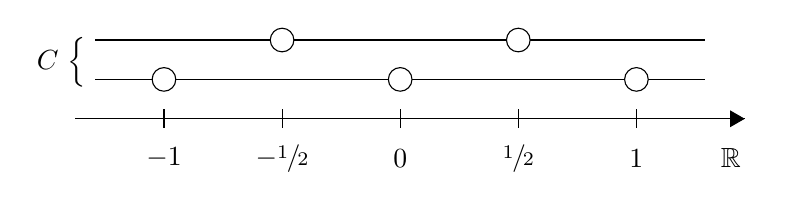
\begin{tikzpicture}
\node (v2) at (4,0.5) {};
\node (v1) at (-4.75,0.5) {};
\draw  (v1) edge (v2);
\draw [-triangle 60] (v1) edge (v2);
\node (v3) at (-4.5,1) {};
\node (v4) at (3.5,1) {};
\draw  (v3) edge (v4);
\node (v5) at (-4.5,1.5) {};
\node (v6) at (3.5,1.5) {};
\draw  (v5) edge (v6);
\draw[fill=white]  (-0.5,1) circle (0.15);
\draw[fill=white]  (-3.5,1) node (v7) {} circle (0.15);
\draw[fill=white]  (2.5,1) circle (0.15);
\draw[fill=white]  (-2,1.5) circle (0.15);
\draw[fill=white]  (1,1.5) circle (0.15);
\draw  (-3.5,0.62) edge (-3.5,0.38);
\draw  (-2,0.62) edge (-2,0.38);
\draw  (-0.5,0.62) edge (-0.5,0.38);
\draw  (2.5,0.62) edge (2.5,0.38);
\draw  (1,0.62) edge (1,0.38);
\node at (-3.5,0) {$-1$};
\node at (-2,0) {$-\sfrac{1}{2}$};
\node at (-0.5,0) {$0$};
\node at (1,0) {$\sfrac{1}{2}$};
\node at (2.5,0) {$1$};
\node at (3.7,0) {$\R$};
\node at (-4.8,1.22) {$C\ \Bigl\{$};
\end{tikzpicture}
\end{figure}

It is clear that removing even one element from $C$ will cause $C$ to fail to be an open cover of $\R$. Therefore, there is no finite subcover of $C$ and hence, $\R$ is not compact.
\ee

\bt
Let $(M,\cO_M)$ and $(N,\cO_N)$ be compact topological spaces. Then $(M\times N,\cO_{M\times N})$ is a compact topological space.
\et

The above theorem easily extends to finite cartesian products. 

\bd
Let $(M,\cO)$ be a topological space and let $C$ be a cover. A \emph{refinement}\index{refinement} of $C$ is a cover $R$ such that:
\bse
\forall \, U \in R : \exists \, V \in C : U \se V .
\ese
\ed
Any subcover of a cover is a refinement of that cover, but the converse is not true in general. A refinement $R$ is said to be:
\bit
\item \emph{open} if $R\se \cO$;
\item \emph{locally finite} if for any $p\in M$ there exists a neighbourhood $U(p)$ such that the set:
\bse
\{U \in R \mid U \cap U(p) \neq \vn\}
\ese
is finite as a set.
\eit

Compactness is a very strong property. Hence often times it does not hold, but a weaker and still useful property, called paracompactness, may still hold.

\bd
A topological space $(M,\cO)$ is said to be \emph{paracompact}\index{topological space!paracompact}\index{paracompactness} if every open cover has an open refinement that is locally finite.
\ed

\bc
If a topological space is compact, then it is also paracompact.
\ec

\bd
A topological space $(M,\cO)$ is said to be \emph{metrisable} if there exists a metric $d$ such that the topology induced by $d$ is precisely $\cO$, i.e.\ $\cO_d=\cO$. 
\ed

\bt[Stone]
Every metrisable space is paracompact.
\et

\be
The space $(\R^d,\cO_\mathrm{std})$ is metrisable since $\cO_\mathrm{std}=\cO_d$ where $d = \|\cdot\|_2$. Hence it is paracompact by Stone's theorem.
\ee

\br
Paracompactness is, informally, a rather natural property since every example of a non-paracompact space looks artificial. One such example is the \emph{long line} (or \emph{Alexandroff line}). To construct it, we first observe that we could ``build'' $\R$ by taking the interval $[0,1)$ and stacking countably many copies of it one after the other. Hence, in a sense, $\R$ is equivalent to $\Z \times [0,1)$. The long line $L$ is defined analogously as $L:\omega_1\times [0,1)$, where $\omega_1$ is an uncountably infinite set. The resulting space $L$ is not paracompact.
\er

\bt
Let $(M,\cO_M)$ be a paracompact space and let $(N,\cO_N)$ be a compact space. Then $M\times N$ (equipped with the product topology) is paracompact.
\et

\bc
Let $(M,\cO_M)$ be a paracompact space and let $(N_i,\cO_{N_i})$ be compact spaces for every $1\leq i \leq n$. Then $M\times N_1\times\cdots\times N_n$ is paracompact.
\ec

\bd
Let $(M,\cO_M)$ be a topological space. A \emph{partition of unity}\index{partition of unity}  of $M$ is a set $\cF$ of continuous maps from $M$ to the interval $[0,1]$ such that for each $p\in M$ the following conditions hold:
\ben
\item[i)] there exists $U(p)$ such that the set $\{f \in \cF \mid \forall \, x \in U(p):f(x)\neq 0\}$ is finite;
\item[ii)] $\sum_{f\in \cF}f(p)=1$.
\een
If $C$ is an open cover, then $\cF$ is said to be \emph{subordinate} to the cover $C$ if:
\bse
\forall \, f \in \cF : \exists \, U \in C : f(x) \neq 0 \imp x \in U .
\ese
\ed

\bt
Let $(M,\cO_M)$ be a Hausdorff topological space. Then $(M,\cO_M)$ is paracompact if, and only if, every open cover admits a partition of unity subordinate to that cover.
\et

\be
Let $\R$ be equipped with the standard topology. Then $\R$ is paracompact by Stone's theorem. Hence, every open cover of $\R$ admits a partition of unity subordinate to that cover. As a simple example, consider $\cF = \{f,g\}$, where:
\bse
f(x) = \left\{ \ba{ll} 0 & \t{ if } x \leq 0\\ x^2 & \t{ if } 0\leq x\leq 1\\ 1 & \t{ if } x \geq 1 \ea \right.
\quad \t{and } \quad
g(x) = \left\{ \ba{ll} 1 & \t{ if } x \leq 0\\ 1-x^2 & \t{ if } 0\leq x\leq 1\\ 0 & \t{ if } x \geq 1 \ea \right. 
\ese
Then $\cF$ is a partition of unity of $\R$. Indeed, $f,g\cl \R \to [0,1]$ are both continuous, condition i) is satisfied since $\cF$ itself is finite, and we have $\forall \, x \in \R : f(x)+g(x)=1$.

Let $C:=\{(-\infty,1),(0,\infty)\}$. Then $C$ is an open cover of $\R$ and since:
\bse
f(x)\neq 0 \imp x \in (0,\infty) \quad \t{and} \quad g(x) \neq 0 \imp x \in (-\infty,1),
\ese
the partition of unity $\cF$ is subordinate to the open cover $C$.
\ee


\subsection{Connectedness and path-connectedness}

\bd
A topological space $(M,\cO)$ is said to be \emph{connected}\index{connectedness}\index{topological space!connected} unless there exist two non-empty, non-intersecting open sets $A$ and $B$ such that $M=A\cup B$.
\ed

\be
Consider $(\R\sm \{0\},\cO_\mathrm{std}|_{\R\sm\{0\}})$, i.e.\ $\R\sm\{0\}$ equipped with the subset topology inherited from $\R$. This topological space is not connected since $(-\infty,0)$ and $(0,\infty)$ are open, non-empty, non-intersecting sets such that $\R\sm\{0\}=(-\infty,0) \cup (0,\infty)$.
\ee

\bt
The interval $[0,1]\se\R$ equipped with the subset topology is connected.
\et

\bt
A topological space $(M,\cO)$ is connected if, and only if, the only subsets that are both open and closed are $\vn$ and $M$.
\et

\bq
\ben
\item[($\imp$)] Suppose, for the sake of contradiction, that there exists $U\se M$ such that $U$ is both open and closed and $U\notin\{\vn,M\}$. Consider the sets $U$ and $M\sm U$. Clearly, we have $U \cap M\sm U = \vn$. Moreover, $M\sm U$ is open since $U$ is closed. Therefore, $U$ and $M\sm U$ are two open, non-empty, non-intersecting sets such that $M = U \cup M \sm U$, contradicting the connectedness of $(M,\cO)$.
\item[($\Leftarrow$)] Suppose that $(M,\cO)$ is not connected. Then there exist open, non-empty, non-intersecting subsets $A,B\se M$ such that $M=A\cup B$. Clearly, $A \neq M$, otherwise we would have $B=\vn$. Moreover, since $B$ is open, $A=M\sm B$ is closed. Hence, $A$ is a set which is both open and closed and $A \notin \{\vn,M\}$.\qedhere
\een
\eq

\bd
A topological space $(M,\cO)$ is said to be \emph{path-connected}\index{path-connectedness}\index{topological space!path-connected} if for every pair of points $p,q\in M$ there exists a continuous curve $\g\cl[0,1]\to M$ such that $\g(0)=p$ and $\g(1)=q$.
\ed

\be
The space $(\R^d,\cO_\mathrm{std})$ is path-connected. Indeed, let $p,q\in\R^d$ and let:
\bse
\g(\l):=p+\l(q-p).
\ese
Then $\g$ is continuous and satisfies $\g(0)=p$ and $\g(1)=q$.
\ee

\be
Let $S:=\{(x,\sin(\tfrac{1}{x}))\mid x\in (0,1]\}\cup \{(0,0)\}$ be equipped with the subset topology inherited from $\R^2$. Then $(S,\cO_\mathrm{std}|_S)$ is connected but not path-connected.
\ee

\bt
If a topological space is path-connected, then it is also connected.
\et

\bq
Let $(M,\cO)$ be path-connected but not connected. Then there exist open, non-empty, non-intersecting subsets $A,B\subset M$ such that $M=A\cup B$. Let $p \in A$ and $q \in B$. Since $(M,\cO)$ is path-connected, there exists a continuous curve $\g\cl[0,1]\to M$ such that $\g(0)=p$ and $\g(1)=q$. Then:
\bse
[0,1] = \mathrm{preim}_\g(M) =  \mathrm{preim}_\g(A\cup B) =  \mathrm{preim}_\g(A)\cup  \mathrm{preim}_\g( B).
\ese
The sets $\mathrm{preim}_\g(A)$ and $ \mathrm{preim}_\g( B)$ are both open, non-empty and non-intersecting, contradicting the fact that $[0,1]$ is connected.
\eq

\subsection{Homotopic curves and the fundamental group}

\bd
Let $(M,\cO)$ be a topological space. Two curves $\g,\delta\cl[0,1]\to M$ such that:
\bse
\g(0)=\delta(0) \quad \t{and} \quad \g(1)=\delta(1)
\ese
are said to be \emph{homotopic}\index{homotopic curves} if there exists a continuous map $h \cl [0,1]\times[0,1]\to M$ such that for all $\l \in [0,1]$:
\bse
h(0,\l) = \g(\l) \quad \t{and} \quad h(1,\l)=\delta(\l).
\ese
\ed

Pictorially, two curves are homotopic if they can be continuously deformed into one another.

\begin{figure}[h!]
\centering
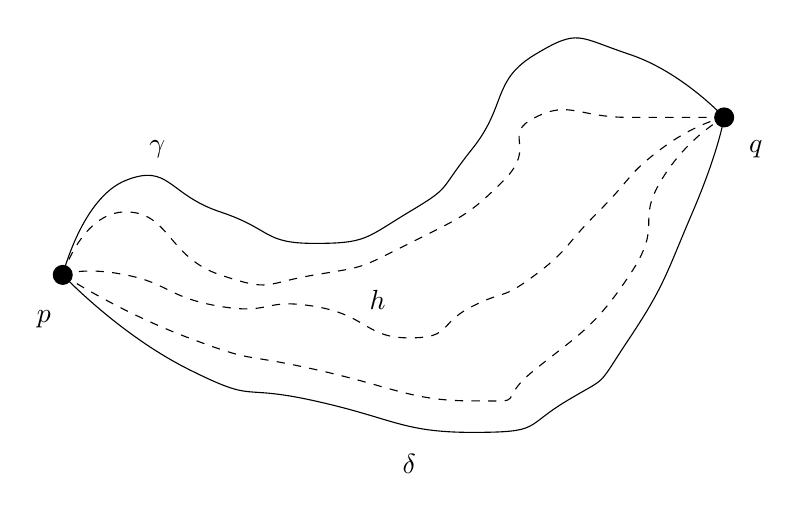
\begin{tikzpicture}[scale=0.8]

\draw  plot[smooth, tension=.999] coordinates {(-3,-0.5) (-2,1) (-0.5,0.5) (1,0) (2.5,0.5) (3.5,1.5) (4.5,3) (6,3) (7.5,2)};

\draw  plot[smooth, tension=.999] coordinates {(-3,-0.5) (-1,-2) (1,-2.5) (3.5,-3) (5,-2.5) (6,-1.5) (7,0.5) (7.5,2)};

\draw[dashed]  plot[smooth, tension=.999] coordinates {(-3,-0.5) (-2,0.5) (-0.5,-0.5) (1,-0.5) (2.5,0) (4,1) (4.5,2) (6,2) (7.5,2)};

\draw[dashed]  plot[smooth, tension=.999] coordinates {(-3,-0.5) (-2,-0.5) (-0.5,-1) (1,-1) (2.5,-1.5) (3.5,-1) (4.5,-0.5) (5.5,0.5) (6.5,1.5) (7.5,2)};

\draw[dashed]  plot[smooth, tension=.999] coordinates {(-3,-0.5) (-1,-1.5) (1,-2) (3.5,-2.5) (4.5,-2) (6,-0.5) (6.5,1) (7.5,2)};

\draw[fill=black]  (-3,-0.5) circle (0.15);
\draw[fill=black]  (7.5,2) circle (0.15);
\node at (-3.3,-1.2) {$p$};
\node at (8,1.5) {$q$};
\node at (-1.5,1.5) {$\g$};
\node at (2,-0.9) {$h$};
\node at (2.5,-3.5) {$\delta$};
\end{tikzpicture}
\end{figure}

\bp
Let $\g \sim \delta :\eqv$ ``$\g$ and $\delta$ are homotopic''. Then, $\sim$ is an equivalence relation.
\ep

\bd
Let $(M,\cO)$ be a topological space. Then, for every $p\in M$, we define the \emph{space of loops} at $p$ by:
\bse
\mathscr{L}_p := \{\g\cl[0,1]\to M \mid \g \t{ is continuous and } \g(0)=\g(1)\}.
\ese
\ed

\bd
Let $\mathscr{L}_p$ be the space of loops at $p\in M$. We define the \emph{concatenation} operation $*\cl \mathscr{L}_p\times\mathscr{L}_p\to\mathscr{L}_p$ by:
\bse
(\g * \delta) (\l):= \left\{ \ba{ll} \g(2\l) & \t{if } 0\leq \l \leq \tfrac{1}{2}\\ \delta(2\l-1) & \t{if } \tfrac{1}{2}\leq \l \leq 1 \ea \right.
\ese
\ed

\bd
Let $(M,\cO)$ be a topological space. The \emph{fundamental group}\index{fundamental group} $\pi_1(p)$\index{$\pi_1(p)$} of $(M,\cO)$ at $p\in M$ is the set:
\bse
\pi_1(p) := \mathscr{L}_p/\!\sim\ = \{[\g] \mid \g \in \mathscr{L}_p\},
\ese
where $\sim$ is the homotopy equivalence relation, together with the map 
\bi{rrCl}
\bullet \cl & \pi_1(p)\times \pi_1(p) &\to &\pi_1(p)\\
&(\g,\delta)&\mapsto & [\g]\bullet[\delta]:=[\g*\delta] .
\ei
\ed

\br
Recall that a group\index{group} is a pair $(G,\bullet)$ where $G$ is a set and $\bullet \cl G\times G \to G$ is a map (also called \emph{binary operation}) such that:
\ben
\item[i)] $\forall \, a,b,c \in G : (a\bullet b)\bullet c = a \bullet (b\bullet c)$;
\item[ii)] $\exists \, e \in G : \forall \, g \in G : g \bullet e = e \bullet g = g$;
\item[iii)] $\forall \, g \in G : \exists \, g^{-1}\in G: g \bullet g^{-1} = g^{-1} \bullet g = e$.
\een
A group is called \emph{abelian (or commutative)} if, in addition, $a\bullet b = b \bullet a$ for all $a,b\in G$.

A \emph{group isomorphism}\index{isomorphism!of groups} between two groups $(G,\bullet)$ and $(H,\circ)$ is a bijection $\phi\cl G \to H$ such that:
\bse
\forall \, a,b \in G:\phi(a \bullet b) = \phi(a)\circ\phi(b).
\ese
If there exists a group isomorphism between $(G,\bullet)$ and $(H,\circ)$, we say that $G$ and $H$ are (group theoretic) isomorphic and we write $G \cong_\mathrm{grp} H$.
\er

The operation $\bullet$ is associative (since concatenation is associative); the neutral element of the fundamental group $(\pi_1(p),\bullet)$ is (the equivalence class of) the constant curve $\g_e$ defined by:
\bi{rrCl}
\g_e \cl & [0,1] & \to & M\\
& \l & \mapsto & \g_e(0) = p
\ei
Finally, for each $[\g]\in\pi_1(p)$, the inverse under $\bullet$ is the element $[-\g]$, where $-\g$ is defined by:
\bi{rrCl}
-\g \cl & [0,1] & \to & M\\
& \l & \mapsto & \g(1-\l)
\ei

All the previously discussed topological properties are ``boolean-valued'', i.e.\ a topological space is either Hausdorff or not Hausdorff, either connected or not connected, and so on. The fundamental group is a ``group-valued'' property, i.e.\ the value of the property is not ``either yes or no'', but a group. 

A property of a topological space is called an \emph{invariant} if any two homeomorphic spaces share the property. A \emph{classification} of topological spaces would be a list of topological invariants such that any two spaces which share these invariants are homeomorphic. As of now, no such list is known. 

\be
The 2-sphere is defined as the set:
\bse
S^2:=\{(x,y,z)\in \R^3\mid x^2+y^2+z^2=1\}
\ese
equipped with the subset topology inherited from $\R^3$. The sphere has the property that all the loops at any point are homotopic, hence the fundamental group (at every point) of the sphere is the trivial group:
\bse
\forall \, p \in S^2 : \pi_1(p) = 1:=\{[\g_e]\}.
\ese
\ee

\be
The cylinder is defined as $C:=\R\times S^1$ equipped with the product topology. A loop in $C$ can either go around the cylinder (i.e.\ around its central axis) or not. If it does not, then it can be continuously deformed to a point (the identity loop). If it does, then it cannot be deformed to the identity loop (intuitively because the cylinder is infinitely long) and hence it is a homotopically different loop. The number of times a loop winds around the cylinder is called the \emph{winding number}\index{winding number}. Loops with different winding numbers are not homotopic. Moreover, loops with different \emph{orientations} are also not homotopic and hence we have:
\bse
\forall \, p \in C : (\pi_1(p),\bullet) \cong_\mathrm{grp}(\Z,+).
\ese
\ee

\be
The 2-torus is defined as the set $T^2:=S^1\times S^1$ equipped with the product topology. A loop in $T^2$ can intuitively wind around the cylinder-like part of the torus as well as around the hole of the torus. That is, there are two independent winding numbers and hence:
\bse
\forall \, p \in T^2 : \pi_1(p) \cong_\mathrm{grp}\Z\times \Z,
\ese
where $\Z\times \Z$ is understood as a group under pairwise addition.
\ee








































% \newpage

% \section{Topological manifolds and bundles}
% \subsection{Topological manifolds}

\bd
A paracompact, Hausdorff, topological space $(M,\cO)$ is called a \emph{$d$-dimensional (topological) manifold}\index{manifold}\index{manifold!topological} if for every point $p\in M$ there exist a neighbourhood $U(p)$ and a homeomorphism $x\cl U(p) \to x(U(p)) \se \R^d$. We also write $\dim M = d$.
\ed

Intuitively, a $d$-dimensional\index{dimension!manifold} manifold is a topological space which locally (i.e.\ around each point) looks like $\R^d$. Note that, strictly speaking, what we have just defined are \emph{real} topological manifolds. We could define \emph{complex} topological manifolds as well, simply by requiring that the map $x$ be a homeomorphism onto an open subset of $\C^d$. 
\bp
Let $M$ be a $d$-dimensional manifold and let $U,V\se M$ be open, with $U\cap V \neq \vn$. If $x$ and $y$ are two homeomorphisms
\bse
x\cl U \to x(U)\se \R^d \qquad \text{and}\qquad y\cl V \to y(V)\se\R^{d'},
\ese
then $d=d'$.
\ep
This ensures that the concept of dimension is indeed well-defined, i.e.\ it is the same at every point, at least on each connected component of the manifold.

\be
Trivially, $\R^d$ is a $d$-dimensional manifold for any $d \geq 1$. The space $S^1$ is a 1-dimensional manifold while the spaces $S^2$, $C$ and $T^2$ are 2-dimensional manifolds.
\ee

\bd
Let $(M,\cO)$ be a topological manifold and let $N \se M$. Then $(N,\cO|_N)$ is called a \emph{submanifold} of $(M,\cO)$ if it is a manifold in its own right.
\ed

\be
The space $S^1$ is a submanifold of $\R^2$ while the spaces $S^2$, $C$ and $T^2$ are submanifolds of $\R^3$. 
\ee

\bd
Let $(M,\cO_M)$ and $(N,\cO_N)$ be topological manifolds of dimension $m$ and $n$, respectively. Then, $(M\times N,\cO_{M\times N})$ is a topological manifold of dimension $m+n$ called the \emph{product manifold}\index{manifold!product}.
\ed

\be
We have $T^2=S^1\times S^1$ not just as topological spaces, but as topological manifolds as well. This is a special case of the $n$-torus:
\bse
T^n := \underbrace{S^1\times S^1 \times \cdots \times S^1}_{\t{$n$ times}},
\ese
which is an $n$-dimensional manifold.
\ee

\be
The cylinder $C=S^1\times \R$ is a $2$-dimensional manifold.
\ee

\subsection{Bundles}

Products are very useful. Very often in physics one intuitively thinks of the product of two manifolds as attaching a copy of the second manifold to each point of the first.  However, not all interesting manifolds can be understood as products of manifolds. A classic example of this is the \emph{M\"obius strip}\index{M\"obius strip}.\footnote{The TikZ code for the M\"obius strip was written by \href{http://pgfplots.net/tikz/examples/author/jake/}{Jake} on \href{https://tex.stackexchange.com/questions/118563/moebius-strip-using-tikz}{TeX.SE}.}
\vspace{-0.1cm}
\begin{center}
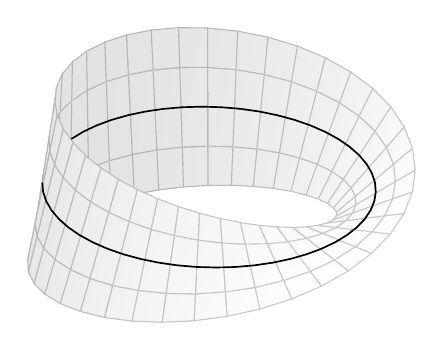
\begin{tikzpicture}
\begin{axis}[
    hide axis,
    view={40}{45}
]
\addplot3 [
    surf, shader=faceted interp,
    point meta=x,
    colormap={slategraywhite}{rgb=(0.89,0.89,0.89) rgb=(1,1,1)},
    samples=40,
    samples y=5,
    %z buffer=sort,
    domain=0:360,
    y domain=-0.5:0.5
] (
    {(1+0.5*y*cos(x/2)))*cos(x)},
    {(1+0.5*y*cos(x/2)))*sin(x)},
    {0.5*y*sin(x/2)});

\addplot3 [
    samples=50,
    domain=-142:184.5, % The domain needs to be adjusted manually, depending on the camera angle, unfortunately
    samples y=0,
    semithick
] (
    {cos(x)},
    {sin(x)},
    {0});
\end{axis}
\end{tikzpicture}
\end{center}
\vspace{-0.6cm}
It looks locally like the finite cylinder $S^1\times [0,1]$, which we can picture as the circle $S^1$ (the thicker line in figure) with the finite interval $[0,1]$ attached to each of its points in a ``smooth'' way. The M\"obius strip has a ``twist'', which makes it globally different from the cylinder.
\bd
A \emph{bundle}\index{bundle} (of topological manifolds) is a triple $(E,\pi,M)$ where $E$ and $M$ are topological manifolds called the \emph{total space} and the \emph{base space} respectively, and $\pi$ is a continuous, surjective map $\pi\cl E \to M$ called the \emph{projection map}.
\ed

We will often denote the bundle $(E,\pi,M)$ by $E\xrightarrow{\,\pi\,}M$.

\bd
Let $E\xrightarrow{\,\pi\,}M$ be a bundle and let $p\in M$. Then, $F_p:=\preim_\pi(\{p\})$ is called the \emph{fibre}\index{fibre} at the point $p$.
\ed

Intuitively, the fibre at the point $p\in M$ is a set of points in $E$ (represented below as a line) attached to the point $p$. The projection map sends all the points is the fibre $F_p$ to the point $p$.

\begin{figure}[h!]
\centering
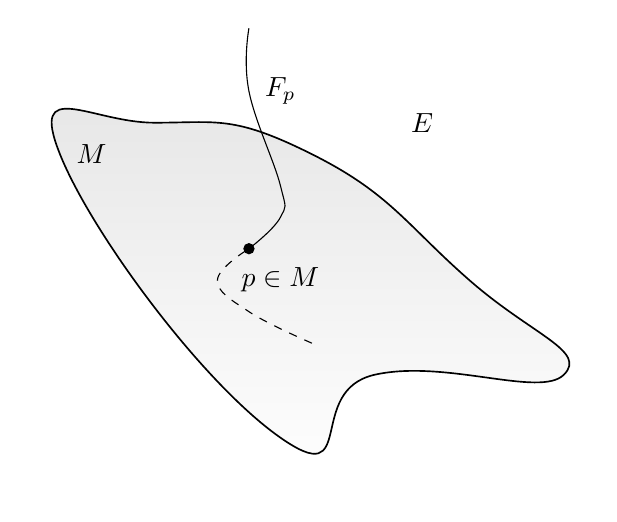
\begin{tikzpicture}[scale=0.8]
\draw[top color=lightergray,bottom color=white,semithick]  plot[smooth cycle, tension=.9] coordinates {(-3,1.5)(-1.5,2) (1,1.5) (3.5,-0.5) (5,-2) (2,-2) (0.5,-3)};
\node (v1) at (0,0) {};
\draw[dashed] plot[smooth, tension=.7] coordinates {(1,-1.5) (0,-1) (-0.5,-0.5) (v1)};
\draw  plot[smooth, tension=.7] coordinates {(v1) (0.5,0.5) (0.5,1) (0,2.5) (0,3.5)};
\draw[fill=black]  (v1) circle (0.08);
\node at (0.5,2.5) {$F_p$};
\node at (2.75,2) {$E$};
\node at (0.5,-0.5) {$p \in M$};
\node at (-2.5,1.5) {$M$};
\end{tikzpicture}
\end{figure}

\be
A trivial example of a bundle is the \emph{product bundle}. Let $M$ and $N$ be manifolds. Then, the triple $(M\times N,\pi,M)$, where:
\bi{rrCl}
\pi \cl & M\times N & \to & M\\
& (p,q) & \mapsto & p
\ei
is a bundle since (one can easily check) $\pi$ is a continuous and surjective map. Similarly, $(M\times N,\pi,N)$ with the appropriate $\pi$, is also a bundle.
\ee

\be
In a bundle, different points of the base manifold may have (topologically) different fibres. For example, consider the bundle $E\xrightarrow{\,\pi\,}\R$ where:
\bse
F_p:=\mathrm{preim}_\pi(\{p\}) \cong_\mathrm{top} \left\{ \ba{ll} S^1 &\t{if }p<0\\
\{p\} & \t{if }p=0\\ {}
[0,1] & \t{if } p>0 \ea \right.
\ese
\ee

\bd
Let $E\xrightarrow{\,\pi\,}M$ be a bundle and let $F$ be a manifold. Then, $E\xrightarrow{\,\pi\,}M$ is called a \emph{fibre bundle}\index{fibre bundle}\index{bundle!fibre}, with (typical) fibre $F$, if:
\bse
\forall \, p \in M : \mathrm{preim}_\pi(\{p\}) \cong_\mathrm{top} F.
\ese
\ed

A fibre bundle is often represented diagrammatically as:
\bse
\begin{tikzcd}
F\ar[r] & E \ar[d,"\pi"]\\
& M
\end{tikzcd}
\ese

\be
The bundle $M\times N\xrightarrow{\,\pi\,}M$ is a fibre bundle with fibre $F:=N$.
\ee

\be
The M\"obius strip is a fibre bundle $E\xrightarrow{\,\pi\,}S^1$, with fibre $F:=[0,1]$, where $E\neq S^1\times[0,1]$, i.e.\ the M\"obius strip is not a product bundle. 
\ee

\be
A $\C$-line bundle over $M$ is the fibre bundle $(E,\pi,M)$ with fibre $\C$. Note that the product bundle $(M\times \C,\pi,M)$ is a $\C$-line bundle over $M$, but a $\C$-line bundle over $M$ need not be a product bundle.
\ee

\bd
Let $E\xrightarrow{\,\pi\,}M$ be a bundle. A map $\s\cl M \to E$ is called a \emph{(cross-)section}\index{section} of the bundle if $\pi \circ \s = \id_M$.
\ed

Intuitively, a section is a map $\s$ which sends each point $p\in M$ to \emph{some} point $\s(p)$ in its fibre $F_p$, so that the projection map $\pi$ takes $\s(p) \in F_p\se E$ back to the point $p\in M$.


\begin{figure}[h!]
\centering
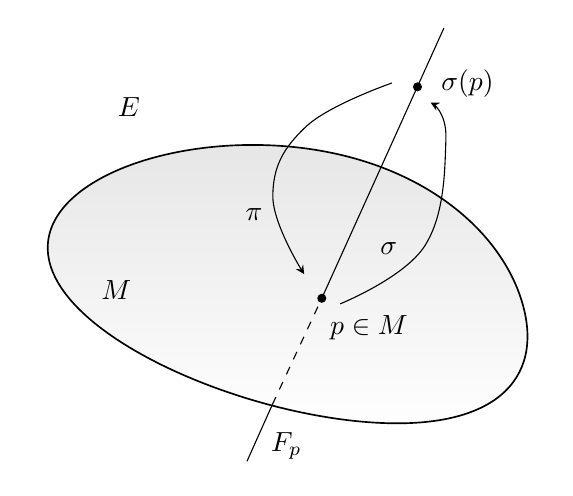
\begin{tikzpicture}[scale=1]
\draw[top color=lightergray,bottom color=white,semithick]  plot[smooth cycle, tension=.99] coordinates {(-2.5,0) (0.5,1.5) (3.5,-0.5) (1.5,-2)};
\draw (0,-2.5) -- (0.3224,-1.7792);
\draw[dashed]  (0.3224,-1.7792) -- (0.9501,-0.4298);
\draw (0.9501,-0.4298)-- (2.5,3);
\node at (0.5,-2.3) {$F_p$};
\node at (1.55,-0.8) {$p \in M$};
\draw[fill=black] (0.9501,-0.4298) circle (0.05);
\draw [->] plot[smooth, tension=.7] coordinates {(1.1834,-0.5006) (2.2576,0.2354) (2.5265,1.5914) (2.3316,2.0564)};
\draw [->] plot[smooth, tension=.7] coordinates {(1.8399,2.3042) (0.7458,1.7472) (0.3281,0.872) (0.7259,-0.1226)};
\node at (0.09,0.6333) {$\pi$};
\node at (1.8,0.2) {$\s$};
\node at (-1.6612,-0.3216) {$M$};
\draw [fill=black] (2.1651,2.2555) circle (0.05);
\node at (2.8,2.3) {$\s(p)$};
\node at (-1.5,2) {$E$};
\end{tikzpicture}
\end{figure}

\be
Let $(M\times F,\pi,M)$ be a product bundle. Then, a section of this bundle is a map:
\bi{rrCl}
\s \cl & M & \to & M\times F\\
& p & \mapsto & (p,s(p))
\ei
where $s\cl M \to F$ is any map.
\ee

\bd
A \emph{sub-bundle}\index{sub-bundle} of a bundle $(E,\pi,M)$ is a triple $(E',\pi',M')$ where $E'\se E$ and $M'\se M$ are submanifolds and $\pi':=\pi|_{E'}$.
\ed

\bd
Let $(E,\pi,M)$ be a bundle and let $N\se M$ be a submanifold. The \emph{restricted bundle}\index{bundle!restricted} (to $N$) is the triple $(E,\pi',N)$ where:
\bse
\pi':=\pi|_{\mathrm{preim}_\pi(N)}
\ese
\ed

\bd
Let $E\xrightarrow{\,\pi\,}M$ and $E'\xrightarrow{\,\pi'\,}M'$ be bundles and let $u\cl E\to E'$ and $v\cl M\to M'$ be maps. Then $(u,v)$ is called a \emph{bundle morphism}\index{bundle morphism} if the following diagram commutes:
\bse
\begin{tikzcd}
E \ar[r,"u"] \ar[d,"\pi"]& E' \ar[d,"\pi'"]\\
M \ar[r,"v"]& M'
\end{tikzcd}
\ese
i.e.\ if $\pi'\circ u = v \circ \pi$.
\ed

If $(u,v)$ and $(u,v')$ are both bundle morphisms, then $v=v'$. That is, given $u$, if there exists $v$ such that $(u,v)$ is a bundle morphism, then $v$ is unique.

\bd
Two bundles $E\xrightarrow{\,\pi\,}M$ and $E'\xrightarrow{\,\pi'\,}M'$ are said to be \emph{isomorphic (as bundles)}\index{bundle!(locally) isomorphic} if there exist bundle morphisms $(u,v)$ and $(u^{-1},v^{-1})$ satisfying:
\bse
\begin{tikzcd}
E \ar[rr,shift left,"u"] \ar[dd,"\pi"']&& E' \ar[ll,shift left,"u^{-1}"]\ar[dd,"\pi'"]\\
&&\\
M \ar[rr,shift left,"v"]&& M' \ar[ll,shift left,"v^{-1}"]
\end{tikzcd}
\ese
Such a $(u,v)$ is called a \emph{bundle isomorphism}\index{isomorphism!of bundles} and we write $E\xrightarrow{\,\pi\,}M  \cong_{\mathrm{bdl}} E'\xrightarrow{\,\pi'\,}M'$.
\ed

Bundle isomorphisms are the structure-preserving maps for bundles.

\bd
A bundle $E\xrightarrow{\,\pi\,}M$ is said to be \emph{locally isomorphic (as a bundle)} to a bundle $E'\xrightarrow{\,\pi'\,}M'$ if for all $p\in M$ there exists a neighbourhood $U(p)$ such that the restricted bundle:
\bse
\mathrm{preim}_\pi(U(p))\xrightarrow{\,\pi|_{\mathrm{preim}_\pi(U(p))}\,}U(p)
\ese
is isomorphic to the bundle $E'\xrightarrow{\,\pi'\,}M'$.
\ed

\bd
A bundle $E\xrightarrow{\,\pi\,}M$ is said to be:
\ben
\item[i)] \emph{trivial}\index{bundle!(locally) trivial} if it is isomorphic to a product bundle;
\item[ii)] \emph{locally trivial} if it is locally isomorphic to a product bundle.
\een
\ed

\be
The cylinder $C$ is trivial as a bundle, and hence also locally trivial.
\ee

\be
The M\"obious strip is not trivial but it is locally trivial.
\ee

From now on, we will mostly consider locally trivial bundles.

\br
In quantum mechanics, what is usually called a ``wave function'' is not a function at all, but rather a section of a $\C$-line bundle over physical space. However, if we assume that the $\C$-line bundle under consideration is locally trivial, then each section of the bundle can be represented (locally) by a map from the base space to the total space and hence it is appropriate to use the term ``wave \emph{function}''. 
\er

\bd
Let $E\xrightarrow{\,\pi\, }M$ be a bundle and let $f\cl M'\to M$ be a map from some manifold $M'$. The \emph{pull-back bundle of} \index{bundle!pull-back}$E\xrightarrow{\,\pi\, }M$ \emph{induced by} $f$ is defined as $E'\xrightarrow{\,\pi'\,}M'$, where:
\bse
E':=\{(m',e)\in M'\times E \mid f(m')=\pi(e)\}
\ese
and $\pi' (m',e) := m'$.
\ed

If $E'\xrightarrow{\,\pi'\,}M'$ is the pull-back bundle of $E\xrightarrow{\,\pi\, }M$ induced by $f$, then one can easily construct a bundle morphism by defining:
\bi{rcCl}
u \cl & E'  & \to & E\\
& (m',e) & \mapsto & e
\ei
This corresponds to the diagram:
\bse
\begin{tikzcd}
E' \ar[d,"\pi'"] \ar[r,"u"] & E\ar[d,"\pi"]\\
M' \ar[r,"f"]& M
\end{tikzcd}
\ese

\br
Sections on a bundle pull back to the pull-back bundle. Indeed, let $E'\xrightarrow{\,\pi'\,}M'$ be the pull-back bundle of $E\xrightarrow{\,\pi\, }M$ induced by $f$.
\bse
\begin{tikzcd}
E' \ar[dd,shift left,"\pi'"] && E\ar[dd,shift left,"\pi"]\\
&&\\
M' \ar[uurr,"\s\circ f"]\ar[uu,shift left,"\s'"]\ar[rr,"f"]&& M\ar[uu,shift left,"\s"]
\end{tikzcd}
\ese
If $\s$ is a section of $E\xrightarrow{\,\pi\, }M$, then $\s \circ f$ determines a map from $M'$ to $E$ which sends each $m'\in M'$ to $\s(f(m')) \in E$. However, since $\s$ is a section, we have:
\bse
\pi(\s(f(m'))= (\pi \circ \s \circ f)(m') = (\id_M\circ f)(m') = f(m')
\ese
and hence $(m',(\s \circ f)(m'))\in E'$ by definition of $E'$. Moreover:
\bse
\pi' (m',(\s \circ f)(m')) = m'
\ese
and hence the map:
\bi{rcCl}
\s' \cl & M'  & \to & E'\\
& m' & \mapsto & (m',(\s \circ f)(m'))
\ei
satisfies $\pi'\circ\s'=\id_{M'}$ and it is thus a section on the pull-back bundle $E'\xrightarrow{\,\pi'\,}M'$.
\er

\subsection{Viewing manifolds from atlases}

\bd
Let $(M,\cO)$ be a $d$-dimensional manifold. Then, a pair $(U,x)$ where $U\in \cO$ and $x\cl U \to x(U) \se \R^d$ is a homeomorphism, is said to be a \emph{chart}\index{chart} of the manifold.
\ed

The \emph{component functions (or maps)}\index{component map}\index{map!component} of $x\cl U\to x(U) \se \R^d$ are the maps:
\bi{rcCl}
x^i \cl & U  & \to & \R\\
& p & \mapsto & \proj_i(x(p))
\ei
for $1\leq i\leq d$, where $\mathrm{proj}_i(x(p))$ is the $i$-th component of $x(p)\in \R^d$. The $x^i(p)$ are called the \emph{co-ordinates}\index{co-ordinates} of the point $p\in U$ with respect to the chart $(U,x)$.

\bd
An \emph{atlas}\index{atlas} of a manifold $M$ is a collection $\mathscr{A}:=\{(U_\a,x_\a)\mid \a \in \mathcal{A}\}$ of charts such that:
\bse
\bigcup_{\a \in \mathcal{A}}U_\a = M. 
\ese
\ed

\bd
Two charts $(U,x)$ and $(V,y)$ are said to be \emph{$\mathcal{C}^0$-compatible} if either $U \cap V = \vn$ or the map:
\bse
y\circ x^{-1}\cl x(U\cap V) \to y(U\cap V)
\ese
is continuous.
\ed

Note that $y\circ x^{-1}$ is a map from a subset of $\R^d$ to a subset of $\R^d$.
\bse
\begin{tikzcd}
& U\cap V \se M \ar[ldd,"x"'] \ar[rdd,"y"]&\\
&&&\\
x(U\cap V) \se \R^d \ar[rr,"y\circ x^{-1}"']& & y(U\cap V)\se \R^d
\end{tikzcd}
\ese

Since the maps $x$ and $y$ are homeomorphisms, the composition map $y \circ x^{-1}$ is also a homeomorphism and hence continuous. Therefore, any two charts on a topological manifold are $\mathcal{C}^0$-compatible. This definition my thus seem redundant since it applies to every pair of charts. However, it is just a ``warm up'' since we will later refine this definition and define the \emph{differentiability} of maps on a manifold in terms of $\mathcal{C}^k$-compatibility of charts. 

\br
The map $y\circ x^{-1}$ (and its inverse $x\circ y^{-1}$) is called the \emph{co-ordinate change map} or \emph{chart transition map}\index{map!transition}.
\er

\bd
A \emph{$\mathcal{C}^0$-atlas} of a manifold is an atlas of pairwise $\mathcal{C}^0$-compatible charts.
\ed

Note that any atlas is also a \emph{$\mathcal{C}^0$-atlas}.

\bd
A $\mathcal{C}^0$-atlas $\mathscr{A}$ is said to be a \emph{maximal atlas} if for every $(U,x)\in\mathscr{A}$, we have $(V,y)\in\mathscr{A}$ for all $(V,y)$ charts that are $\mathcal{C}^0$-compatible with $(U,x)$.
\ed

\be
Not every $\mathcal{C}^0$-atlas is a maximal atlas. Indeed, consider $(\R,\cO_\mathrm{std})$ and the atlas $\mathscr{A}:=(\R,\id_\R)$. Then $\mathscr{A}$ is not maximal since $((0,1),\id_\R)$ is a chart which is $\mathcal{C}^0$-compatible with $(\R,\id_\R)$ but $((0,1),\id_\R) \notin \mathscr{A}$.
\ee

We can now look at ``objects on'' topological manifolds from two points of view. For instance, consider a curve on a $d$-dimensional manifold $M$, i.e.\ a map $\g\cl \R\to M$. We now ask whether this curve is continuous, as it should be if models the trajectory of a particle on the ``physical space'' $M$.

A first answer is that $\g\cl \R \to M$ is continuous if it is continuous as a map between the topological spaces $\R$ and $M$.

However, the answer that may be more familiar to you from undergraduate physics is the following. We consider only a portion (open subset $U$) of the physical space $M$ and, instead of studying the map $\g\cl\mathrm{preim}_\g(U)\to U$ directly, we study the map:
\bse
x\circ \g\cl \mathrm{preim}_\g(U) \to x(U) \se \R^d,
\ese
where $(U,x)$ is a chart of $M$. More likely, you would be checking the continuity of the co-ordinate maps $x^i\circ \g$, which would then imply the continuity of the ``real'' curve $\g\cl\mathrm{preim}_\g(U)\to U$ (real, as opposed to its co-ordinate representation).
\bse
\begin{tikzcd}
&& y(U)\se\R^d\\
&&\\
\mathrm{preim}_\g(U)\se\R \ar[rr,"\g"] \ar[ddrr,"x\circ \g"] \ar[uurr,"y\circ \g"]&& U\se M \ar[dd,"x"] \ar[uu,"y"'] \\
&&\\
&& x(U)\se\R^d \ar[uuuu,bend right=65,"y\circ x^{-1}"']
\end{tikzcd}
\ese
At some point you may wish to use a different ``co-ordinate system'' to answer a different question. In this case, you would chose a different chart $(U,y)$ and then study the map $y\circ \g$ or its co-ordinate maps. Notice however that some results (e.g.\ the continuity of $\g$) obtained in the previous chart $(U,x)$ can be immediately ``transported'' to the new chart $(U,y)$ via the chart transition map $y\circ x^{-1}$. Moreover, the map $y\circ x^{-1}$ allows us to, intuitively speaking, forget about the inner structure (i.e.\ $U$ and the maps $\g$, $x$ and $x$) which, in a sense, is the real world, and only consider $\mathrm{preim}_\g(U)\se \R$ and $x(U),y(U)\se\R^d$ together with the maps between them, which is our representation of the real world.















% \newpage

% \section{Differentiable structures: definition and classification}
% 
\subsection{Adding structure by refining the (maximal) atlas}

We saw previously that for a topological manifold $(M,\cO)$, the concept of a $C^0$-atlas was fully redundant since every atlas is also a $C^0$-atlas. We will now generalise the notion of a $C^0$-atlas, or more precisely, the notion of $C^0$-compatibility of charts, to something which is non-trivial and non-redundant.

\begin{definition}
An atlas $\mathscr{A}$ for a topological manifold is called a {\scalebox{0.75}\FiveFlowerOpen}-\emph{atlas} if any two charts $(U,x), (V,y) \in \mathscr{A}$ are {\scalebox{0.75}\FiveFlowerOpen}-compatible.
\end{definition}

In other words, either $U\cap V = \vn$ or if $U\cap V \neq \vn$, then the transition map $y\circ x^{-1}$ from $x(U\cap V)$ to $y(U\cap V)$ must be {\scalebox{0.75}\FiveFlowerOpen}.
\bse
\begin{tikzcd}
& U\cap V \se M \ar[ldd,"x"'] \ar[rdd,"y"]&\\
&&&\\
x(U\cap V) \se \R^{\dim M} \ar[rr,"y\circ x^{-1}"']& & y(U\cap V)\se \R^{\dim M}
\end{tikzcd}
\ese
Before you think Dr Schuller finally went nuts, the symbol {\scalebox{0.75}\FiveFlowerOpen} is being used as a placeholder for any of the following:
\begin{itemize}
\item ${\scalebox{0.75}\FiveFlowerOpen} = C^0$: this just reduces to the previous definition;
\item ${\scalebox{0.75}\FiveFlowerOpen} = C^k$: the transition maps are $k$-times continuously differentiable as maps between open subsets of $\R^{\dim M}$;
\item ${\scalebox{0.75}\FiveFlowerOpen} = C^\infty$: the transition maps are smooth (infinitely many times differentiable); equivalently, the atlas is $C^k$ for all $k\geq 0$;
\item ${\scalebox{0.75}\FiveFlowerOpen} = C^\omega$: the transition maps are (real) analytic, which is stronger than being smooth;
\item ${\scalebox{0.75}\FiveFlowerOpen} =$ complex: if $\dim M$ is even, $M$ is a \emph{complex manifold} if the transition maps are continuous and satisfy the Cauchy-Riemann equations; its complex dimension is $\tfrac{1}{2}\dim M$.
\end{itemize}

As an aside, if you haven't met the Cauchy-Riemann equations yet, recall than since $\R^2$ and $\C$ are isomorphic as sets, we can identify the function 
\bi{rcCl}
f\cl & \R^2 & \to     & \R^2 \\
     &(x,y) & \mapsto & (u(x,y),v(x,y))
\ei
where $u,v \cl \R^2\to\R$, with the function
\bi{rcCl}
f\cl & \C & \to     & \C \\
     &x+\mathrm{i}y & \mapsto & u(x,y)+\mathrm{i}v(x,y).
\ei
If $u$ and $v$ are real differentiable at $(x_0,y_0)$, then $f=u+\mathrm{i}v$ is complex differentiable at $z_0=x_0+\mathrm{i}y_0$ if, and only if, $u$ and $v$ satisfy
\bse
\frac{\partial u}{\partial x}(x_0,y_0)= \frac{\partial v}{\partial y}(x_0,y_0) \quad \land \quad \frac{\partial u}{\partial y}(x_0,y_0)= - \frac{\partial v}{\partial x}(x_0,y_0),
\ese
which are known as the Cauchy-Riemann equations\index{Cauchy-Riemann eqns}. Note that differentiability in the complex plane is a much stronger condition than differentiability over the real numbers. If you want to know more, you should take a course in complex analysis or function theory.

We now go back to manifolds.

\begin{theorem}[Whitney] Any maximal $C^k$-atlas, with $k\geq 1$, contains a $C^\infty$-atlas. Moreover, any two maximal $C^k$-atlases that contain the same $C^\infty$-atlas are identical.
\end{theorem}

An immediate implication is that if we can find a $C^1$-atlas for a manifold, then we can also assume the existence of a $C^\infty$-atlas for that manifold. This is not the case for topological manifolds in general: a space with a $C^0$-atlas may not admit any $C^1$-atlas. But if we have at least a $C^1$-atlas, then we can obtain a $C^\infty$-atlas simply by removing charts, keeping only the ones which are $C^\infty$-compatible.

Hence, for the purposes of this course, we will not distinguish between $C^k$ ($k\geq 1$) and $C^\infty$-manifolds in the above sense.

We now give the explicit definition of a $C^k$-manifold.

\bd
A $C^k$\emph{-manifold} is a triple $(M,\cO,\mathscr{A})$, where $(M,\cO)$ is a topological manifold and $\mathscr{A}$ is a maximal $C^k$-atlas.
\ed

\br 
A given topological manifold can carry different incompatible atlases.
\er

Note that while we only defined compatibility of charts, it should be clear what it means for two atlases of the same type to be compatible.

\bd
Two {\scalebox{0.75}\FiveFlowerOpen}-atlases $\mathscr{A}$, $\mathscr{B}$ are \emph{compatible} if their union $\mathscr{A}\cup\mathscr{B}$ is again a {\scalebox{0.75}\FiveFlowerOpen}-atlas, and are incompatible otherwise.
\ed

Alternatively, we can define the compatibility of two atlases in terms of the compatibility of any pair of charts, one from each atlas.

\be
Let $(M,\cO)=(\R,\cO_\mathrm{std})$. Consider the two atlases $\mathscr{A}=\{(\R,\id_\R)\}$ and $\mathscr{B}=\{(\R,x)\}$, where $x\cl a \mapsto \sqrt[3]{a}$. Since they both contain a single chart, the compatibility condition on the transition maps is easily seen to hold (in both cases, the only transition map is $\id_\R$). Hence they are both $C^\infty$-atlases.

Consider now $\mathscr{A}\cup\mathscr{B}$. The transition map $\id_\R\circ x^{-1}$ is the map $a\mapsto a^3$, which is smooth. However, the other transition map, $x\circ\id_\R^{-1}$, is the map $x$, which is not even differentiable once (the first derivative at $0$ does not exist). Consequently, $\mathscr{A}$ and $\mathscr{B}$ are not even $C^1$-compatible.
\ee

The previous example shows that we can equip the real line with (at least) two different incompatible $C^\infty$-structures. This looks like a disaster as it implies that there is an arbitrary choice to be made about which differentiable structure to use. Fortunately, the situation is not as bad as it looks, as we will see in the next sections.

\subsection{Differentiable manifolds}

\bd
Let $\phi\cl M\to N$ be a map, where $(M,\cO_M,\mathscr{A}_M)$ and $(N,\cO_N,\mathscr{A}_N)$ are $C^k$-manifolds. Then $\phi$ is said to be ($C^k$-)\emph{differentiable at} $p\in M$ if for some charts $(U,x)\in\mathscr{A}_M$ with $p\in U$ and $(V,y)\in\mathscr{A}_N$ with $\phi(p)\in V$, the map $y\circ\phi\circ x^{-1}$ is $k$-times continuously differentiable at $x(p)\in x(U)\se\R^{\dim M}$ in the usual sense.
\bse
\begin{tikzcd}
U\se M \ar[rr,"\phi"] \ar[dd,"x"] && V\se N \ar[dd,"y"]\\
&&\\
x(U)\se\R^{\dim M}\ar[rr,"y\circ\phi\circ x^{-1}"] && y(V)\se\R^{\dim N}
\end{tikzcd}
\ese
\ed
The above diagram shows a typical theme with manifolds. We have a map $\phi\cl M\to N$ and we want to define some property of $\phi$ at $p\in M$ analogous to some property of maps between subsets of $\R^d$. What we typically do is consider some charts $(U,x)$ and $(V,y)$ as above and define the desired property of $\phi$ at $p\in U$ in terms of the corresponding property of the downstairs map $y\circ\phi\circ x^{-1}$ at the point $x(p)\in\R^d$.

Notice that in the previous definition we only require that \emph{some} charts from the two atlases satisfy the stated property. So we should worry about whether this definition depends on which charts we pick. In fact, this ``lifting'' of the notion of differentiability from the chart representation of $\phi$ to the manifold level is well defined.

\bp
The definition of differentiability is well defined.
\ep

\bq
We want to show that if $y\circ\phi\circ x^{-1}$ is differentiable at $x(p)$ for some $(U,x)\in\mathscr{A}_M$ with $p\in U$ and $(V,y)\in\mathscr{A}_N$ with $\phi(p)\in V$, then $\widetilde y\circ\phi\circ \widetilde x^{-1}$ is differentiable at $\widetilde x(p)$ for all charts $(\widetilde U,\widetilde x)\in\mathscr{A}_M$ with $p\in \widetilde U$ and $(\widetilde V,\widetilde y)\in\mathscr{A}_N$ with $\phi(p)\in \widetilde V$.
\bse
\begin{tikzcd}
\widetilde x(U\cap\widetilde U)\se\R^{\dim M}\ar[rr,"\widetilde y\circ\phi\circ \widetilde x^{-1}"] && \widetilde y(V\cap\widetilde V)\se\R^{\dim N}\\
&&\\
U\cap\widetilde U\se M \ar[rr,"\phi"] \ar[dd,"x"] \ar[uu,"\widetilde x"'] && V\cap\widetilde V\se N \ar[dd,"y"] \ar[uu,"\widetilde y"']\\
&&\\
x(U\cap\widetilde U)\se\R^{\dim M}\ar[rr,"y\circ\phi\circ x^{-1}"] \ar[uuuu,bend left=70,"\widetilde x\circ x^{-1}"]&& y(V\cap\widetilde V)\se\R^{\dim N} \ar[uuuu,bend right=70,"\widetilde y\circ y^{-1}"']
\end{tikzcd}
\ese
Consider the map $\widetilde x\circ x^{-1}$ in the diagram above. Since the charts $(U,x)$ and $(\widetilde U,\widetilde x)$ belong to the same $C^k$-atlas $\mathscr{A}_M$, by definition the transition map $\widetilde x\circ x^{-1}$ is $C^k$-differentiable as a map between subsets of $\R^{\dim M}$, and similarly for $\widetilde y\circ y^{-1}$. We now notice that we can write:
\bse
\widetilde y\circ\phi\circ \widetilde x^{-1} = (\widetilde y\circ y^{-1})\circ(y\circ\phi\circ x^{-1})\circ(\widetilde x\circ x^{-1})^{-1}
\ese
and since the composition of $C^k$ maps is still $C^k$, we are done.
\eq
This proof shows the significance of restricting to $C^k$-atlases. Such atlases only contain charts for which the transition maps are $C^k$, which is what makes our definition of differentiability of maps between manifolds well defined.

The same definition and proof work for smooth ($C^\infty$) manifolds, in which case we talk about \emph{smooth maps}. As we said before, this is the case we will be most interested in.

\subsection{Classification of differentiable structures}

\bd
Let $\phi\cl M \to N$ be a bijective map between smooth manifolds. If both $\phi$ and $\phi^{-1}$ are smooth, then $\phi$ is said to be a \emph{diffeomorphism}\index{diffeomorphism}.
\ed

Diffeomorphisms are the structure preserving maps between smooth manifolds. 

\bd
Two manifolds $(M,\cO_M,\mathscr{A}_M)$, $(N,\cO_N,\mathscr{A}_N)$ are said to be \emph{diffeomorphic} if there exists a diffeomorphism $\phi\cl M\to N$ between them. We write $M \cong_\text{diff}N$.
\ed

Note that if the differentiable structure is understood (or irrelevant), we typically write $M$ instead of the triple $(M,\cO_M,\mathscr{A}_M)$.

\br
Being diffeomorphic is an equivalence relation. In fact, it is customary to consider diffeomorphic manifolds to be \emph{the same} from the point of view of differential geometry. This is similar to the situation with topological spaces, where we consider homeomorphic spaces to be the same from the point of view of topology. This is typical of all structure preserving maps.
\er

Armed with the notion of diffeomorphism, we can now ask the following question: how many smooth structures on a given topological space are there, up to diffeomorphism?

The answer is quite surprising: it depends on the dimension of the manifold!

\begin{theorem}[Radon-Moise]
Let $M$ be a manifold with $\dim M = 1, 2$, or $3$. Then there is a unique smooth structure on $M$ up to diffeomorphism.
\end{theorem}

Recall that in a previous example, we showed that we can equip $(\R,\cO_\mathrm{std})$ with two incompatible atlases $\mathscr{A}$ and $\mathscr{B}$. Let $\mathscr{A}_\mathrm{max}$ and $\mathscr{B}_\mathrm{max}$ be their extensions to maximal atlases, and consider the smooth manifolds $(\R,\cO_\mathrm{std},\mathscr{A}_\mathrm{max})$ and  $(\R,\cO_\mathrm{std},\mathscr{B}_\mathrm{max})$. Clearly, these are different manifolds, because the atlases are different, but since $\dim \R=1$, they must be diffeomorphic.

The answer to the case $\dim M > 4$ (we emphasize $\dim M \neq 4$) is provided by \emph{surgery theory}. This is a collection of tools and techniques in topology with which one obtains a new manifold from given ones by performing surgery on them, i.e.\ by cutting, replacing and gluing parts in such a way as to control topological invariants like the fundamental group. The idea is to understand all manifolds in dimensions higher than 4 by performing surgery systematically. In particular, using  surgery theory, it has been shown that there are only finitely many smooth manifolds (up to diffeomorphism) one can make from a topological manifold.

This is not as neat as the previous case, but since there are only finitely many structures, we can still enumerate them, i.e.\ we can write an exhaustive list.

While finding all the differentiable structures may be difficult for any given manifold, this theorem has an immediate impact on a physical theory that models spacetime as a manifold. For instance, some physicists believe that spacetime should be modelled as a $10$-dimensional manifold (we are neither proposing nor condemning this view). If that is indeed the case, we need to worry about which differentiable structure we equip our 10-dimensional manifold with, as each different choice will likely lead to different predictions. But since there are only finitely many such structures, physicists can, at least in principle, devise and perform finitely many experiments to distinguish between them and determine which is the right one, if any.

We now turn to the special case $\dim M = 4$. The result is that if $M$ is a non-compact topological manifold, then there are uncountably many non-diffeomorphic smooth structures that we can equip $M$ with. In particular, this applies to $(\R^4,\cO_\mathrm{std})$.

In the compact case there are only partial results. By way of example, here is one such result.

\bp
If $(M,\cO)$, with $\dim M = 4$, has $b_2>18$, where $b_2$ is the second Betti number, then there are countably many non-diffeomorphic smooth structures that we can equip $(M,\cO)$ with. 
\ep

Betti numbers are defined in terms of homology groups, but intuitively we have:
\begin{itemize}
\item $b_0$ is the number of connected components a space has;
\item $b_1$ is the number of circular (1-dimensional) holes a space has;
\item $b_2$ is the number of 2-dimensional holes a space has;
\end{itemize}
and so on. Hence if a manifold has a number of 2-dimensional holes greater than 18, then there only countably many structures that we can choose from, but they are still infinitely many.












% \newpage

% \section{Tensor space theory I: over a field}
% \subsection{Vector spaces}

We begin with a quick review of vector spaces.

\bd
An \emph{(algebraic) field} is a triple $(K,+,\cdot)$, where $K$ is a set and $+,\cdot$ are maps $K\times K \to K$ satisfying the following axioms:
\begin{itemize}
\item $(K,+)$ is an abelian group, i.e.
\ben
\item[i)] $\forall \, a,b,c \in K : (a+b)+c=a+(b+c)$;
\item[ii)] $\exists \, 0 \in K : \forall \, a \in K : a+0=0+a=a$;
\item[iii)] $\forall \, a \in K : \exists \, {-a} \in K : a+(-a)=(-a)+a=0$;
\item[iv)] $\forall \, a,b \in K : a+b=b+a$;
\een
\item $(K^*,\cdot)$, where $K^*=K\sm\{0\}$, is an abelian group, i.e.
\ben
\item[v)] $\forall \, a,b,c \in K^* : (a\cdot b)\cdot c=a\cdot (b\cdot c)$;
\item[vi)] $\exists \, 1 \in K^* : \forall \, a \in K^* : a\cdot 1=1\cdot a=a$;
\item[vii)] $\forall \, a \in K^* : \exists \, a^{-1} \in K^* : a\cdot a^{-1}=a^{-1} \cdot a=1$;
\item[viii)] $\forall \, a,b \in K^* : a\cdot b=b\cdot a$;
\een
\item the maps $+$ and $\cdot$ satisfy the distributive property:
\ben
\item[ix)] $\forall \, a,b,c \in K : (a+ b)\cdot c=a\cdot c + b\cdot c$.
\een
\end{itemize}
\ed

\br
In the above definition, we included axiom iv for the sake of clarity, but in fact it can be proven starting from the other axioms.
\er

\br
A weaker notion that we will encounter later is that of a \emph{ring}. This is also defined as a triple $(R,+,\cdot)$, but we do not require axiom vi, vii and viii to hold. If a ring satisfies axiom vi, it is called a \emph{unital ring}, and if it satisfies axiom viii, it is called a \emph{commutative ring}. We will mostly consider unital rings, a call them just rings.
\er

\be
The triple $(\Z,+,\cdot)$ is a commutative, unital ring. However, it is not a field since $1$ and $-1$ are the only two elements which admit an inverse under multiplication.
\ee

\be
The sets $\Q$, $\R$, $\C$ are all fields under the usual $+$ and $\cdot$ operations.
\ee

\be
An example of a non-commutative ring is the set of real $m\times n$ matrices $M_{m\times n}(\R)$ under the usual operations.
\ee

\bd
Let $(K,+,\cdot)$ be a field. A $K$\emph{-vector space}\index{vector space}, or \emph{vector space over $K$} is a triple $(V,\oplus,\odot)$, where $V$ is a set and 
\bi{rl}
\oplus &\cl V\times V \to V\\
\odot  &\cl K\times V \to V
\ei
are maps satisfying the following axioms:
\begin{itemize}
\item $(V,\oplus)$ is an abelian group;
\item the map $\odot$ is an \emph{action} of $K$ on $(V,\oplus)$:
\ben
\item[i)] $\forall \, \lambda \in K : \forall \, v,w \in V : \lambda\odot(v\oplus w)=(\lambda\odot v)\oplus (\lambda\odot w)$;
\item[ii)] $\forall \, \lambda,\mu \in K : \forall \, v \in V : (\lambda+\mu)\odot v= (\lambda \odot v) \oplus (\mu \odot v)$;
\item[iii)] $\forall \, \lambda,\mu \in K : \forall \, v \in V : (\lambda\cdot\mu)\odot v= \lambda \odot (\mu \odot v)$;
\item[iv)] $\forall \, v \in V : 1\odot v = v$.
\een
\end{itemize}
\ed

Vector spaces are also called \emph{linear spaces}. Their elements are called \emph{vectors}, while the elements of $K$ are often called \emph{scalars}, and the map $\odot$ is called \emph{scalar multiplication}. You should already be familiar with the various vector space constructions from your linear algebra course. For example, recall:

\bd
Let $(V,\oplus,\odot)$ be a vector space over $K$ and let $U\se V$ be non-empty. Then we say that $(U,\oplus|_{U\times U},\odot|_{K\times U})$ is a \emph{vector subspace} of $(V,\oplus,\odot)$ if:
\ben
\item[i)] $\forall \, u_1,u_2\in U : u_1\oplus u_2 \in U$;
\item[ii)] $\forall \, u\in U : \forall \, \lambda \in K: \lambda\odot u \in U$.
\een
More succinctly, if $\forall\,u_1,u_2\in U:\forall \, \lambda \in K: (\lambda\odot u_1)\oplus u_2\in U$. 
\ed

Also recall that if we have $n$ vector spaces over $K$, we can form the $n$-fold Cartesian product of their underlying sets and make it into a vector space over $K$ by defining the operations $\oplus$ and $\odot$ componentwise.

As usual by now, we will look at the structure preserving maps between vector spaces.

\bd
Let $(V,\oplus,\odot)$, $(W,\boxplus,\boxdot)$ be vector spaces over the same field $K$ and let $f\cl V\to W$ be a map. We say that $f$ is a \emph{linear map}\index{linear map} if for all $u_1,u_2\in V$ and all $\lambda \in K$
\bse
f((\lambda\odot u_1)\oplus u_2) = (\lambda\boxdot f( u_1))\boxplus f(u_2).
\ese
\ed

From now on, we will drop the special notation for the vector space operations and suppress the dot for scalar multiplication. For instance, we will write the equation above as $f(\lambda u_1+u_2)=\lambda f(u_1)+f(u_2)$, hoping that this will not cause any confusion.

\bd
A bijective linear map is called a \emph{linear isomorphism} of vector spaces. Two vector spaces are said to be \emph{isomorphic} is there exists a linear isomorphism between them. We write $V\cong_\mathrm{vec}W$.
\ed

\br
Note that, unlike what happens with topological spaces, the inverse of a bijective linear map is automatically linear, hence we do not need to specify this in the definition of linear isomorphism.
\er

\bd
Let $V$ and $W$ be vector spaces over the same field $K$. Define the set
\bse
\mathrm{Hom}(V,W)\index{$\mathrm{Hom}(V,W)$} := \{f \mid f\cl V\xrightarrow{\sim}W \},
\ese
where the notation $ f\cl V\xrightarrow{\sim}W$ stands for ``$f$ is a linear map from $V$ to $W$''.
\ed
The hom-set $\mathrm{Hom}(V,W)$ can itself be made into a vector space over $K$ by defining:
\bi{rcCc}
\diamondplus \cl &\mathrm{Hom}(V,W) \times \mathrm{Hom}(V,W) &\to &\mathrm{Hom}(V,W)\\
& (f,g) & \mapsto & f \diamondplus g
\ei
where
\bi{rcCl}
f \diamondplus g \cl &V  &\to &W\\
& v & \mapsto & (f \diamondplus g)(v) := f(v)+g(v),
\ei 
and
\bi{rcCc}
\diamonddot \cl &K \times \mathrm{Hom}(V,W) &\to &\mathrm{Hom}(V,W)\\
& (\lambda,f) & \mapsto & \lambda \diamonddot f
\ei
where
\bi{rcCl}
\lambda \diamonddot f \cl &V  &\to &W\\
& v & \mapsto & (\lambda \diamonddot f)(v) := \lambda f(v).
\ei 
It is easy to check that both $f \diamondplus g$ and $\lambda \diamonddot f$ are indeed linear maps from $V$ to $W$. For instance, we have:
\bi{rCl"s}
(\lambda \diamonddot f)(\mu v_1+v_2) & = &  \lambda f(\mu v_1+v_2) & (by definition)\\
& = &  \lambda (\mu f( v_1)+f(v_2)) & (since $f$ is linear)\\
& = &  \lambda \mu f( v_1)+\lambda f(v_2) & (by axioms i and iii)\\
& = & \mu \lambda f( v_1)+\lambda f(v_2) & (since $K$ is a field)\\
& = & \mu (\lambda \diamonddot f)( v_1)+(\lambda \diamonddot f)(v_2) & 
\ei
so that $\lambda \diamonddot f\in \mathrm{Hom}(V,W)$. One should also check that $\diamondplus$ and $\diamonddot$ satisfy the vector space axioms.

\br
Notice that in the definition of vector space,none of the axioms require that $K$ necessarily be a field. In fact, just a (unital) ring would suffice. Vector spaces over rings, however, have vastly different properties than ordinary vector spaces, and indeed they have a name of their own. They are called \emph{modules} over a ring, and we will meet them later.

For the moment, it is worth pointing out that everything we have done so far applies equally well to modules over a ring, up to and including the definition of $\mathrm{Hom}(V,W)$. However, if we try to make $\mathrm{Hom}(V,W)$ into a module, we run into trouble. Notice that in the derivation above, we used the fact the multiplication in a field is commutative. But this is not the case in general in a ring.
\er

The following are commonly used terminology.

\bd
Let $V$ be a vector space. An \emph{endomorphism} of $V$ is a linear map $V\to V$. We write $\mathrm{End}(V):=\mathrm{Hom}(V,V)$.
\ed

\bd
Let $V$ be a vector space. An \emph{automorphism} of $V$ is a linear isomorphism $V\to V$. We write $\mathrm{Aut}(V):=\{f \in \mathrm{End}(V) \mid f \text{ is an isomorphism}\}$.
\ed

\br
Note that, unlike $\mathrm{End}(V)$, $\mathrm{Aut}(V)$ is \emph{not} a vector space as was claimed in lecture. It however a group under the operation of composition of linear maps.
\er

\bd
Let $V$ be a vector space over $K$. The \emph{dual} vector space to $V$ is $V^*:=\mathrm{Hom}(V,K)$, where $K$ is considered as a vector space over itself.
\ed

The dual vector space to $V$ is the vector space of linear maps from $V$ to the underlying field $K$, which are variously called \emph{linear functionals}, \emph{covectors}, or \emph{one-forms} on $V$. The dual plays a very important role, in that from a vector space and its dual, we will construct the tensor products.

\subsection{Tensors and tensor spaces}

\bd
Let $V$, $W$, $Z$ be vector spaces over $K$. A map $f\cl V\times W \to Z$ is said to be \emph{bilinear} if
\begin{itemize}
\item $\forall \, w\in W:\forall \, v_1,v_2\in V: \forall \,\lambda \in K : f(\lambda v_1+v_2,w)=\lambda f(v_1,w)+f(v_2,w)$;
\item $\forall \, v\in V:\forall \, w_1,w_2\in W: \forall \,\lambda \in K : f(v,\lambda w_1+w_2)=\lambda f(v,w_1)+f(v,w_2)$;
\end{itemize}
i.e.\ if the maps $v\mapsto f(v,w)$, for any fixed $w$, and $w\mapsto f(v,w)$, for any fixed $v$, are both linear as maps $V\to Z$ and $W\to Z$, respectively.
\ed

\br
Compare this with the definition of a linear map $f\cl V\times W \xrightarrow{\sim} Z$:
\bse
\forall \, x,y\in V \times W : \forall \, \lambda \in K : f(\lambda x+y)=\lambda f(x)+f(y).
\ese
More explicitly, if $x=(v_1,w_1)$ and $y = (v_2,w_2)$, then:
\bse
f(\lambda (v_1,w_1)+(v_2,w_2))=\lambda f((v_1,w_1))+f((v_2,w_2)).
\ese
A bilinear map out of $V\times W$ is \emph{not} the same as a linear map out of $V\times W$. In fact, bilinearity is just a special kind of non-linearity.
\er

\be
The map $f\cl \R^2\to \R$ given by $(x,y)\mapsto x+y$ is linear but not bilinear, while the map $(x,y)\mapsto xy$ is bilinear but not linear.
\ee

We can immediately generalize the above to define \emph{multilinear} maps out of a Cartesian product of vector spaces.

\bd
Let $V$ be a vector space over $K$. A \emph{$(p,q)$-tensor} $T$ on $V$ is a multilinear map
\bse
T\cl \underbrace{V^*\times\cdots \times V^*}_{p \text{ copies}} \times \underbrace{V \times \cdots \times V}_{q \text{ copies}} \to K.
\ese
We write
\bse
T^p_q V := \underbrace{V\otimes\cdots \otimes V}_{p \text{ copies}} \otimes \underbrace{V^* \otimes \cdots \otimes V^*}_{q \text{ copies}} := \{T\mid T \text{ is a $(p,q)$-tensor on }V\}. 
\ese
\ed

\br
By convention, a $(0,0)$ on $V$ is just an element of $K$, and hence $T^0_0V=K$.
\er

\br
Note that to define $T^p_q V$ as a set, we should be careful and invoke the principle of restricted comprehension, i.e.\ we should say where the $T$s are coming from. In general, say we want to build a set of maps $f\cl A\to B$ satisfying some property $p$. Recall that the notation $f\cl A \to B$ is hiding the fact that is a relation (indeed, a functional relation), and a relation between $A$ and $B$ is a subset of $A\times B$. Therefore, we ought to write:
\bse
\{f\in \cP(A\times B)\mid f\cl A\to B \text{ and } p(f)\}.
\ese
In the case of $T^p_q V$ we have:
\bse
T^p_q V := \big\{T \in \cP\big(\underbrace{V^*\times\cdots \times V^*}_{p \text{ copies}} \times \underbrace{V \times \cdots \times V}_{q \text{ copies}} \times K\big) \mid  T \text{ is a $(p,q)$-tensor on }V\big\},
\ese
although we will not write this down every time.
\er

The set $T^p_q V$ can be equipped with a $K$-vector space structure by defining

\bi{rrCl}
\oplus\cl &T^p_q V \times T^p_q V &\to &T^p_q V\\
& (T,S) & \mapsto & T \oplus S
\ei
and
\bi{rrCl}
\odot \cl &K \times T^p_q V &\to &T^p_q V\\
& (\lambda,T) & \mapsto & \lambda \odot T,
\ei
where $T \oplus S$ and $\lambda \odot T$ are defined pointwise, as we did with $\mathrm{Hom}(V,W)$.

We now define an important way of obtaining a new tensor from two given ones.

\bd
Let $T\in T^p_q V$ and $S\in T^r_s V$. We define the \emph{tensor product} of $T$ and $S$ to be $T\otimes S\in T^{p+r}_{q+s}V$ where:
\bi{rl}
(T\otimes S)(v_1,\ldots,v_p,v_{p+1},\ldots,v_{p+s},\omega_1,&\ldots,\omega_q,\omega_{q+1},\ldots,\omega_{q+s})\\
:=T(v_1,\ldots,v_p,\omega_1,&\ldots,\omega_q)S(v_{p+1},\ldots,v_{p+s},\omega_{q+1},\ldots,\omega_{q+s}),
\ei
with $v_i\in V$ and $\omega_i\in V^*$.
\ed

Some examples are in order.

\be
\ben[label=\alph*)]
\item $T^0_1 V := \{T\mid T\cl V \xrightarrow{\sim} K\} = \mathrm{Hom}(V,K) =: V^*$. Note that here multilinear is the same as linear since the maps only have one argument.
\item $T^1_1V\equiv V\otimes V^*:=\{T\mid T\text{ is a bilinear map }V^*\times V \to K\}$. We claim that this is the same as $\mathrm{End}(V^*)$. Indeed, given $T\in  V\otimes V^*$, we can construct $\widehat T \in \mathrm{End}(V^*)$ as follows:
\bi{rrCl}
\widehat T \cl &V^* &\xrightarrow{\sim}& V^*\\
& \omega & \mapsto & T(-,\omega)
\ei
where, for any fixed $\omega$, we have
\bi{rrCl}
T (-,\omega) \cl &V &\xrightarrow{\sim}& K\\
& v & \mapsto & T(v,\omega).
\ei
The linearity of both $\widehat T$ and $T(-,\omega)$ follows immediately from the bilinearity of $T$. Hence $T(-,\omega)\in V^*$ for all $\omega$, and $\widehat T \in \mathrm{End}(V^*)$. This correspondence is invertible, since can reconstruct $T$ from $\widehat T$ by defining
\bi{rrCl}
T  \cl &V \times V^* &\to & K\\
& (v,\omega) & \mapsto & T(v,\omega):=(\widehat T(\omega))(v).
\ei
The correspondence is in fact linear, hence an isomorphism, and thus \bse
T^1_1V\cong_\mathrm{vec}\mathrm{End}(V^*).
\ese
\een
Other examples we would like to consider are
\ben[label=\alph*),start=3]
\item $T^0_1 V \stackrel{?}{\cong}_\mathrm{vec} V$. While you will find this stated as true in physics textbook, but in fact it not true in general.
\item $T^1_1 V \stackrel{?}{\cong}_\mathrm{vec} \mathrm{End}(V)$. This is also not true in general.
\item $(V^*)^* \stackrel{?}{\cong}_\mathrm{vec} V$. This only holds if $V$ is finite dimensional.
\een
\ee
The definition of dimension hinges on the notion of a basis. Given a vector space Without any additional structure, the only notion of basis that we can define is a so-called Hamel basis.

\bd
Let $(V,+,\cdot)$ be a vector space over $K$. A subset $\mathcal{B}\se V$ is called a \emph{Hamel basis}\index{Hamel basis} for $V$ if 
\begin{itemize}
\item every finite subset $\{b_1,\ldots,b_N\}$ of $\mathcal{B}$ is linearly independent, i.e.\
\bse
\sum_{i=1}^N \lambda^ib_i = 0 \ \imp \ \lambda^1 = \cdots = \lambda^N = 0;
\ese
\item $\forall \, v \in V : \exists \, v^1,\ldots,v^M\in K : \exists \, b_1,\ldots,b_M \in \mathcal{B}:v=\ds \sum_{i=1}^Mv^ib_i$.
\end{itemize}
\ed
\br
We can write the second condition more succinctly by defining
\bse
\mathrm{span}(\mathcal{B}) := \bigg\{\sum_{i=1}^n\lambda^ib_i \ \Big| \ \lambda^i\in K \land b_i\in \mathcal{B} \land n\geq 1\bigg\}
\ese
and thus writing $\forall \, v \in V : v \in \mathrm{span}(\mathcal{B})$.
\er
\br
Note that we have been using superscripts for the elements of $K$, and these should not be confused with exponents.
\er
\bd
Let $V$ be a vector space. The \emph{dimension} of $V$ is $\dim V := |\mathcal{B}|$, where $\mathcal{B}$ is a Hamel basis for $V$.
\ed
Even though we will not prove it, it is the case that every Hamel basis for a given vector space has the same cardinality, and hence the notion of dimension is well defined.

\begin{theorem}
If $\dim V < \infty$, then $(V^*)^*\cong_\mathrm{vec}V$.
\end{theorem}

\br
It is not hard to show that $(V^*)^*\cong_\mathrm{vec}V$ implies $T^0_1 V \cong_\mathrm{vec} V$ and $T^1_1 V \cong_\mathrm{vec} \mathrm{End}(V)$. So the last two hold in finite dimensions, but they need not hold in infinite dimensions.
\er

\br
While a choice of basis often simplifies things, when defining new objects it is important to do so without making reference to a basis. If we do define something in terms of a basis (e.g.\ the dimension of a vector space), then we have to check that the thing is well defined, i.e.\ it does not depend on which basis we choose. Some people say: \textit{``A gentleman only chooses a basis if he must.''}
\er

If $V$ is finite dimensional, then $V^*$ is also finite dimensional and $V\cong_\mathrm{vec}V^*$. Moreover, given a basis $\mathcal{B}$ of $V$, there is a spacial basis of $V^*$ associated to $\mathcal{B}$.

\bd
Let $V$ be a finite dimensional vector space with basis $\mathcal{B}=\{e_1,\ldots,e_{\dim V}\}$. The \emph{dual basis} to $\mathcal{B}$ is the unique basis $\mathcal{B'}=\{f^1,\ldots,f^{\dim V}\}$ of $V^*$ such that
\bse
\forall \, 1\leq i,j \leq \dim V :\quad  f^i(e_j) = \delta^i_j := \begin{cases}1 \quad \text{if }i=j\\0 \quad \text{if }i\neq j\end{cases}
\ese
\ed

Once we have a basis $\mathcal{B}$, the expansion of $v\in V$ in terms of elements of $\mathcal{B}$ is, in fact, unique. Hence we can meaningfully speak of the \emph{components} of $v$ in the basis $\mathcal{B}$. The notion of coordinates can also be generalised to the case of tensors.

\bd
Let $V$ be a finite dimensional vector space over $K$ with basis $\mathcal{B}=\{e_1,\ldots,e_{\dim V}\}$ and let $T\in T^p_qV$. We define the \emph{components} of $T$ in the basis $\mathcal{B}$ to be the numbers
\bse
T^{a_1\ldots a_p}_{\phantom{a_1\ldots a_p}b_1\ldots b_q} := T(f^{a_1},\ldots,f^{a_p},e_{b_1},\ldots,e_{b_q})\in K,
\ese
where $1\leq a_i,b_j\leq \dim V$ and $\{f^1,\ldots,f^{\dim V}\}$ is the dual basis to $\mathcal{B}$.
\ed

Just as with vectors, the components completely determine the tensor. Indeed, we can reconstruct the tensor from its components by using the basis:
\bse
T = \underbrace{\sum_{a_1=1}^{\dim V}\!\cdots\!\sum_{b_q=1}^{\dim V}}_{p+q \text{ sums}} T^{a_1\ldots a_p}_{\phantom{a_1\ldots a_p}b_1\ldots b_q} e_{a_1}\otimes\cdots\otimes e_{a_p} \otimes f^{b_1}\otimes \cdots\otimes f^{b_q},
\ese
where the $e_{a_i}$s are understood as elements of $T^1_0V\cong_\mathrm{vec}V$ and the $f^{b_i}s$ as elements of $T^0_1V\cong_\mathrm{vec}V^*$. Note that each summand is a $(p,q)$-tensor and the (implicit) multiplication between the components and the tensor product is the scalar multiplication in $T^p_q V$.

\subsubsection*{Change of basis}

Let $V$ be a vector space over $K$ with $d=\dim V < \infty$ and let $\{e_1,\ldots,e_d\}$ be a basis of $V$. Consider a new basis $\{\widetilde e_1,\ldots,\widetilde e_d\}$. Since the elements of the new basis are also elements of $V$, we can expand them in terms of the old basis. We have:
\bse
\widetilde e_i = \sum_{j=1}^d A^j_{\phantom{j} i}\, e_j \qquad \text{for }1\leq i \leq d.
\ese
for some $A^j_{\phantom{j}i}\in K$. Similarly, we have
\bse
e_i = \sum_{j=1}^d B^j_{\phantom{j} i}\, \widetilde e_j \qquad \text{for }1\leq i \leq d.
\ese
for some $B^j_{\phantom{j}i}\in K$. It is a standard linear algebra result that the matrices $A$ and $B$, with entries $A^j_{\phantom{j}i}$ and $B^j_{\phantom{j}i}$ respectively, are invertible and, in fact, $A^{-1}=B$.

\subsection{Notational conventions}

\subsubsection*{Einstein's summation convention}
From now on, we will employ the Einstein's summation convention, which consists in suppressing the summation sign when the indices to be summed over each appear once as a subscript and once as a superscript in the same term. For example, we write
\bse
v=v^ie_i \qquad \text{and} \qquad T=T^{ij}_{\phantom{ij}k}e_i\otimes e_j \otimes f^k 
\ese
instead of
\bse
v=\sum_{i=1}^dv^ie_i \qquad \text{and} \qquad T=\sum_{i=1}^d\sum_{j=1}^d\sum_{k=1}^d
T^{ij}_{\phantom{ij}k}e_i\otimes e_j \otimes f^k.
\ese
The ranges over which the indices run are usually understood and not written out. The convention on which indices go upstairs and which downstairs (which we have already been using) is that:
\begin{itemize}
\item the basis vectors of $V$ carry downstairs indices;
\item the basis vectors of $V^*$ carry upstairs indices;
\item all other placements are enforced by the Einstein's summation convention.
\end{itemize}
For example, since the components of a vector must multiply the basis vectors and be summed over, the Einstein's summation convention requires that they carry upstair indices.

\be
Using the summation convention, we have:
\ben[label=\alph*)]
\item $f^a(v) = f^a(v^be_b)=v^bf^a(e_b)=v^b\delta^a_b=v^a$;
\item $\omega(e_b)=(\omega_af^a)(e_b)=\omega_af^a(e_b)=\omega_b$;
\item $\omega(v)=\omega_af^a(v^be_b)=\omega_av^a$;
\een
where $v\in V$, $\omega \in V^*$, $\{e_i\}$ is a basis of $V$ and $\{f^j\}$ is the dual basis.
\ee

\br
The Einstein's summation convention should only be used when dealing with linear spaces and multilinear maps. The reason for this is the following. Consider a map $\phi\cl V\times W \to Z$, and let $v=v^ie_i\in V$ and $w=w^i\widetilde e_i\in W$. Then we have:
\bse
\phi(v,w) = \phi\,\bigg({\color{gray}\sum_{i=1}^d}v^ie_i,{\color{gray}\sum_{j=1}^{\widetilde{d}}} w^j\widetilde e_j\bigg) = {\color{gray}\sum_{i=1}^d \sum_{j=1}^{\widetilde{d}}}\phi(v^ie_i,w^j\widetilde e_j)= {\color{gray}\sum_{i=1}^d \sum_{j=1}^{\widetilde{d}}}v^iw^j\phi(e_i,\widetilde e_j).
\ese
Note that by suppressing the greyed out summation signs, the second and third term above are indistinguishable. But this is only true if $\phi$ is bilinear! Hence the summation convention should not be used (at least, not without extra care) in other areas of mathematics.
\er

\br
Having chosen a basis for $V$ and the dual basis for $V^*$, it is very tempting to think of $v=v^ie_i\in V$ and $\omega=\omega_if^i\in V^*$ as $d$-tuples of numbers. In order to distinguish them, one may choose to write vectors as \emph{columns} of numbers and covectors as \emph{rows} of numbers:
\bse
v =v^ie_i \quad \leftrightsquigarrow\quad v\ \hat{=} \left(
\ba{c}
v^1\\
\vdots\\
v^d
\ea
\right)
\ese
and
\bse
\omega =\omega_if^i \quad \leftrightsquigarrow\quad \omega \ \hat{=} \ (\omega_1,\ldots,\omega_d).
\ese
Given $\phi\in\mathrm{End}(V)\cong_\mathrm{vec}T^1_1V$, recall that we can write $\phi = \phi^i_{\phantom{i}j}\, e_i\otimes f^j$, where $\phi^i_{\phantom{i}j}:=\phi(f^i,e_j)$ are the components of $\phi$ with respect to the chosen basis. It is then also very tempting to think of $\phi$ as a square array of numbers:
\bse
\phi = \phi^i_{\phantom{i}j}\, e_i\otimes f^j \quad \leftrightsquigarrow\quad \phi \ \hat{=} \left(
\ba{cccc}
\phi^1_{\phantom{1}1} & \phi^1_{\phantom{1}2} & \cdots & \phi^1_{\phantom{1}d}\\
\phi^2_{\phantom{2}1} & \phi^2_{\phantom{2}2} & \cdots & \phi^2_{\phantom{2}d}\\
\vdots & \vdots & \ddots & \vdots\\
\phi^d_{\phantom{d}1} & \phi^d_{\phantom{d}2} & \cdots & \phi^d_{\phantom{d}d} 
\ea
\right)
\ese
The convention here is to think of the $i$ index on $\phi^i_{\phantom{i}j}$ as a \emph{row index}, and of $j$ as a \emph{column index}.
\er

We cannot stress enough that this is pure convention. Its usefulness stems from the following example.

\be
If $\dim V<\infty$, then we have $\mathrm{End}(V)\cong_\mathrm{vec}T^1_1V$. Explicitly, if $\phi \in \mathrm{End}(V)$, we can think of $\phi \in T^1_1V$, using the same symbol, as
\bse
\phi(\omega,v):=\omega(\phi(v)).
\ese
Hence the components of $\phi\in\mathrm{End}(V)$ are $\phi^a_{\phantom{a}b}:=f^a(\phi(e_b))$. 

Now consider $\phi,\psi\in\mathrm{End}(V)$. Let us determine the components of $\phi\circ \psi$. We have:
\bi{rCl}
(\phi\circ \psi)^a_{\phantom{a}b} &:=& (\phi\circ \psi)(f^a,e_b)\\
&:=&f^a( (\phi\circ \psi)(e_b))\\
&=& f^a( (\phi(\psi(e_b)))\\
&=& f^a(\phi(\psi^m_{\phantom{m}b}\,e_m))\\
&=& \psi^m_{\phantom{m}b} f^a( \phi(e_m))\\
&:=& \psi^m_{\phantom{m}b}\, \phi^a_{\phantom{a}m} .
\ei
The multiplication in the last line is the multiplication in the field $K$, and since that's commutative, we have $\psi^m_{\phantom{m}b}\, \phi^a_{\phantom{a}m}  = \phi^a_{\phantom{a}m} \, \psi^m_{\phantom{m}b}$. However, in light of the convention introduced in the previous remark, the latter is preferable. Indeed, if we think of the superscripts as row indices and of the subscripts as column indices, then $\phi^a_{\phantom{a}m} \, \psi^m_{\phantom{m}b}$ is the entry in row $a$, column $b$, of the matrix product $\phi\psi$.

Similarly, $\omega(v)=\omega_mv^m$ can be thought of as the \emph{dot product} $\omega \cdot v\equiv\omega^Tv$, and
\bse
\phi(v,w)=w_a\,\phi^a_{\phantom{a}b}\,v^b \quad   \leftrightsquigarrow\quad \omega^T\phi v.
\ese
The last expression is could mislead you into thinking that the transpose is a ``good'' notion, but in fact it is not. It is very bad notation. It almost pretends to be basis independent, but it is not at all.

The moral of the story is that you should try your best \emph{not} to think of vectors, covectors and tensors as arrays of numbers. Instead, always try to understand them from the abstract, intrinsic, component-free point of view.
\ee

\subsubsection*{Change of components under a change of basis}

Recall that if $\{e_a\}$ and $\{\widetilde e_a\}$ are basis of $V$, we have
\bse
\widetilde e_a=A^b_{\phantom{b}a}e_b \qquad \text{and}  \qquad e_a=B^m_{\phantom{m}a}\widetilde e_m,
\ese
with $A^{-1}=B$. Note that in index notation, the equation $AB=I$ reads $A^a_{\phantom{a}m}B^m_{\phantom{m}b}=\delta^a_b$.

We now investigate how the components of vectors and covectors change under a change of basis. 
\ben[label=\alph*)]
\item Let $v=v^ae_a=\widetilde v^a\widetilde e_a\in V$. Then:
\bse
v^a = f^a(v) = f^a(\widetilde v^b\widetilde e_b) = \widetilde v^b
f^a(\widetilde e_b) = \widetilde v^b f^a(A^m_{\phantom{m}b}e_m) = A^m_{\phantom{m}b} \widetilde v^bf^a(e_m)=A^a_{\phantom{a}b} \widetilde v^b.
\ese
\item Let $\omega = \omega_af^a = \widetilde \omega_a\widetilde f^a  \in V^*$. Then:
\bse
\omega_a := \omega(e_a) = \omega(B^m_{\phantom{m}a}\widetilde e_m) = B^m_{\phantom{m}a}\omega(\widetilde e_m) = B^m_{\phantom{m}a}\widetilde \omega_m .
\ese
\een
Summarising, for $v\in V$, $\omega \in V^*$ and $\widetilde e_a=A^b_{\phantom{b}a}e_b$, we have:
\bi{rClcrCl}
v^a & = & A^a_{\phantom{a}b} \widetilde v^b &\qquad & \omega_a &= & B^b_{\phantom{b}a}\widetilde \omega_b \\
\widetilde v^a & = & B^a_{\phantom{a}b}  v^b & & \widetilde \omega_a &= & A^b_{\phantom{b}a}\omega_b 
\ei
The result for tensors is a combination of the above, depending on the type of tensor.
\ben
\item[c)] Let $T\in T^p_qV$. Then:
\bse
T^{a_1\ldots a_p}_{\phantom{a_1\ldots a_p}b_1\ldots b_q} = A^{a_1}_{\phantom{a_1}m_1}\cdots A^{a_p}_{\phantom{a_p}m_p} B^{n_1}_{\phantom{n_1}b_1} \cdots B^{n_q}_{\phantom{n_q}b_q} \widetilde T^{m_1\ldots m_p}_{\phantom{m_1\ldots m_p}n_1\ldots n_q},
\ese
i.e.\ the upstair indices transform like vector indices, and the downstair indices transform like covector indices. 
\een

\subsection{Determinants}

In your previous course on linear algebra, you may have met the determinant of a square matrix as a number calculated by applying a mysterious rule. Using the mysterious rule, you may have shown, with a lot of work, that for example, if we exchange two rows or two columns, the determinant changes sign. But, as we have seen, matrices are the result of pure convention. Hence, one more polemic remark is in order.

\br
Recall that, if $\phi \in T^1_1V$, then we can arrange the components $\phi^a_{\phantom{a}b}$ in matrix form:
\bse
\phi = \phi^a_{\phantom{a}b}\, e_a\otimes f^b \quad \leftrightsquigarrow\quad \phi \ \hat{=} \left(
\ba{cccc}
\phi^1_{\phantom{1}1} & \phi^1_{\phantom{1}2} & \cdots & \phi^1_{\phantom{1}d}\\
\phi^2_{\phantom{2}1} & \phi^2_{\phantom{2}2} & \cdots & \phi^2_{\phantom{2}d}\\
\vdots & \vdots & \ddots & \vdots\\
\phi^d_{\phantom{d}1} & \phi^d_{\phantom{d}2} & \cdots & \phi^d_{\phantom{d}d} 
\ea
\right)
\ese
Similarly, if we have $g\in T^0_2V$, its components are $g_{ab}:=g(e_a,e_b)$ and we can write
\bse
g = g_{ab}\, f^a\otimes f^b \quad \leftrightsquigarrow\quad g \ \hat{=} \left(
\ba{cccc}
g_{11} & g_{12} & \cdots & g_{1d}\\
g_{21} & g_{22} & \cdots & g_{2d}\\
\vdots & \vdots & \ddots & \vdots\\
g_{d1} & g_{d2} & \cdots & g_{dd} 
\ea
\right)
\ese
Needless to say that these two objects could not be more different if they tried. Indeed
\begin{itemize}
\item $\phi$ is an endomorphism of $V$; the first index in $\phi^a_{\phantom{a}b}$ transforms like a vector index, while the second index transforms like a covector index;
\item $g$ is a \emph{bilinear form} $V$; both indices in $g_{ab}$ transform like covector indices.
\end{itemize}
In linear algebra, you may have seen the two different transformation laws for these objects:
\bse
\phi \to A^{-1}\phi A \qquad \text{and} \qquad g \to A^TgA,
\ese
where $A$ is the change of basis matrix. However, once we fix a basis, the matrix representations of these two objects are indistinguishable. It is then very tempting to think that what we can do with a matrix, we can just as easily do with another matrix. For instance, if we have a rule to calculate the determinant of a square matrix, we should be able to apply it to both of the above matrices.

However, the notion of determinant is \emph{only} defined for endomorphisms. The only way to see this is to give a basis-independent definition, i.e.\ a definition that does not involve the ``components of a matrix''.  
\er

We will need some preliminary definitions.

\bd
Let $M$ be a set. A \emph{permutation} of $M$ is a bijection $M\to M$.
\ed

\bd
The \emph{symmetric group} of order $n$, denoted $S_n$, is the set of permutations of $\{1,\ldots,n\}$ under the operation of functional composition.
\ed

\bd
A \emph{transposition} is a permutation which exchanges two elements, keeping all other elements fixed.  
\ed

\bp
Every permutation $\pi\in S_n$ can be written as a product (composition) of transpositions in $S_n$.
\ep
While this decomposition is not unique, for each given $\pi \in S_n$, the number of transpositions in its decomposition is always either even or odd. Hence, we can define the \emph{sign} of $\pi \in S_n$ as:
\bse
\mathrm{sgn}(\pi) := \begin{cases}+1 \qquad &\text{if $\pi$ is the product of an even number of transpositions}\\-1 \qquad &\text{if $\pi$ is the product of an odd number of transpositions.}\end{cases}
\ese

\bd
Let $V$ be a $d$-dimensional vector space. An $n$-\emph{form} on $V$, with $0\leq n \leq d$, is a $(0,n)$-tensor $\omega$ that is \emph{totally antisymmetric}, i.e.\
\bse
\forall \, \pi \in S_n : \ \omega(v_1,v_2,\ldots,v_n) = \mathrm{sgn}(\pi)\, \omega(v_{\pi(1)},v_{\pi(2)},\ldots,v_{\pi(n)}). 
\ese
\ed
Note that a $0$-form is scalar, and a $1$-form is a covector.
























% \newpage

%  \section{Differential structures: the pivotal concept of tangent vector spaces}
%  \subsection{Tangent spaces to a manifold}

In this section, whenever we say ``manifold'', we mean a (real) $d$-dimensional differentiable manifold, unless we explicitly say otherwise. We will also suppress the differentiable structure in the notation.

\bd
Let $M$ be a manifold. We define the infinite-dimensional vector space over $\R$ with underlying set
\bse
\mathcal{C}^\infty(M)\index{$\mathcal{C}^\infty(M)$} := \{f\cl M \to \R \mid f\text{ is smooth}\}
\ese
and operations defined pointwise, i.e.\ for any $p\in M$,
\bi{rCl}
(f+g)(p) & := & f(p)+g(p)\\
(\lambda f)(p) & := & \lambda f(p).
\ei
\ed
A routine check shows that this is indeed a vector space. We can similarly define $\mathcal{C}^\infty(U)$, with $U$ an open subset of $M$.

\bd
A \emph{smooth curve}\index{smooth curve} on $M$ is a smooth map $\gamma\cl \R \to M$, where $\R$ is understood as a $1$-dimensional manifold.
\ed
This definition also applies to smooth maps $I\to M$ for an open interval $I\se \R$.

\bd
Let $\gamma\cl\R\to M$ be a smooth curve through $p\in M$; w.l.o.g.\ %\footnote{without loss of generality} 
let $\gamma(0)=p$. The \emph{directional derivative operator}\index{directional derivative operator} at $p$ along $\gamma$ is the linear map
\bi{rrCl}
X_{\gamma,p}\cl & \mathcal{C}^\infty(M) & \xrightarrow{\sim} & \R\\
& f & \mapsto & (f\circ\gamma)'(0),
\ei
where $\R$ is understood as a $1$-dimensional vector space over the field $\R$.
\ed
Note that $f\circ\gamma$ is a map $\R\to\R$, hence we can calculate the usual derivative and evaluate it at $0$.

\br
In differential geometry, $X_{\gamma,p}$ is called the \emph{tangent vector}\index{tangent vector} to the curve $\gamma$ at the point $p\in M$. Intuitively, $X_{\gamma,p}$ is the velocity $\gamma$ at $p$. Consider the curve $\delta(t):=\gamma(2t)$, which is the same curve parametrised twice as fast. We have, for any $f\in \mathcal{C}^\infty(M)$:
\bse
X_{\delta,p}(f) = (f\circ\delta)'(0)=2(f\circ\gamma)'(0)=2 X_{\gamma,p}(f)
\ese
by using the chain rule. Hence $X_{\gamma,p}$ scales like a velocity should.
\er

\bd
Let $M$ be a manifold and $p\in M$. The \emph{tangent space}\index{tangent space}\index{$T_pM$} to $M$ at $p$ is the vector space over $\R$ with underlying set
\bse
T_pM := \{X_{\gamma,p}\mid \gamma \text{ is a smooth curve through }p\},
\ese
addition
\bi{rrCl}
\oplus\cl & T_pM\times T_pM & \to & T_pM \\
& (X_{\gamma,p},X_{\delta,p}) & \mapsto & X_{\gamma,p}\oplus X_{\delta,p},
\ei
and scalar multiplication
\bi{rrCl}
\odot\cl & \R\times T_pM & \to & T_pM \\
& (\lambda,X_{\gamma,p}) & \mapsto & \lambda \odot X_{\gamma,p},
\ei
both defined pointwise, i.e. for any $f\in \mathcal{C}^\infty(M)$,
\bi{rCl}
(X_{\gamma,p}\oplus X_{\delta,p})(f) & := & X_{\gamma,p}(f) + X_{\delta,p}(f)\\
(\lambda \odot X_{\gamma,p})(f) & := & \lambda X_{\gamma,p}(f).
\ei
\ed

Note that the outputs of these operations do not look like elements in $T_pM$, because they are not of the form $X_{\sigma,p}$ for some curve $\sigma$. Hence, we need to show that the above operations are, in fact, well-defined.

\bp
Let $X_{\gamma,p}, X_{\delta,p}\in T_pM$ and $\lambda \in \R$. Then, we have $X_{\gamma,p}\oplus X_{\delta,p}\in T_pM$ and $\lambda \odot X_{\gamma,p}\in T_pM$.
\ep

Since the derivative is a local concept, it is only the behaviour of curves near $p$ that matters. In particular, if two curves $\gamma$ and $\delta$ agree on a neighbourhood of $p$, then $X_{\gamma,p}$ and $X_{\delta,p}$ are the same element of $T_pM$. Hence, we can work \emph{locally} by using a chart on $M$.

\bq
Let $(U,x)$ be a chart on $M$, with $U$ a neighbourhood of $p$. 
\ben
\item[i)] Define the curve
\bse
\sigma (t):= x^{-1} ( (x\circ \gamma) (t) + (x \circ \delta)(t)-x(p)).
\ese
Note that $\sigma$ is smooth since it is constructed via addition and composition of smooth maps and, moreover:
\bi{rCl}
\sigma (0)&=& x^{-1} ( x(\gamma (0)) + x (\delta(0))-x(p))\\
&=& x^{-1} ( x(p)) + x (p)-x(p))\\
&=& x^{-1} (x(p))\\
&=& p.
\ei
% \bse
% \begin{tikzcd}
% \preim_\gamma(U) \se \R \ar[r,"\gamma"]  & U \ar[r, bend left,"x"]  & x(U)\se \R^{\dim M} \ar[l, bend left,"x^{-1}"]
% \end{tikzcd}
% \ese
Thus $\sigma$ is a smooth curve through $p$. Let $f\in \mathcal{C}^\infty(U)$ be arbitrary. Then we have
\bi{rCl}
X_{\sigma,p}(f)& := & (f\circ \sigma)'(0)\\
& = & [f\circ x^{-1} \circ ( (x\circ \gamma) + (x \circ \delta) -x(p))]'(0)\\
 \intertext{where $(f\circ x^{-1}) \cl \R^d\to \R$ and $((x\circ \gamma) + (x \circ \delta) -x(p))\cl\R\to\R^d$, so by the multivariable chain rule}
& = & [\partial_a(f\circ x^{-1})(x(p))]\, ( (x^a\circ \gamma) + (x^a \circ \delta) -x^a(p))'(0)\\
 \intertext{where $x^a$, with $1\leq a \leq d$, are the component functions of $x$, and since the derivative is linear, we get}
 & = & [\partial_a(f\circ x^{-1})(x(p))]\, ( (x^a\circ \gamma)'(0) + (x^a \circ \delta)'(0))  \\
& = & (f \circ x^{-1} \circ x \circ \gamma)'(0) + (f \circ x^{-1} \circ x \circ \delta)'(0) \\
& = & (f \circ \gamma)'(0) + (f \circ \delta)'(0) \\
& =: & (X_{\gamma,p}\oplus X_{\delta,p})(f).
\ei
Therefore $X_{\gamma,p}\oplus X_{\delta,p}= X_{\sigma,p} \in T_pM$.
\item[ii)] The second part is straightforward. Define $\sigma(t) := \gamma(\lambda t)$. This is again a smooth curve through $p$ and we have:
\bi{rCl}
X_{\sigma,p}(f) & := & (f \circ \sigma)'(0)\\ 
 & = & f'( \sigma(0))\,\sigma'(0)\\ 
 & = & \lambda f'( \gamma(0))\,\gamma'(0) \\ 
 & = & \lambda (f\circ \gamma)'(0) \\
 & := & (\lambda \odot X_{\gamma,p} )(f)  
\ei
for any $f\in \mathcal{C}^\infty(U)$. Hence $\lambda \odot X_{\gamma,p}=X_{\sigma,p}\in T_pM$. \qedhere
\een
\eq

\br
We now give a slightly different (but equivalent) definition of $T_pM$. Consider the set of smooth curves
\bse
S=\{\gamma\cl I\to M \mid \text{with } I\se \R \text{ open, } 0\in I \text{ and } \gamma(0)=p\}
\ese
and define the equivalence relation $\sim$ on $S$
\bse
\gamma \sim \delta \ :\eqv \ (x\circ \gamma)'(0) = (x\circ \delta)'(0)  
\ese
for some (and hence every) chart $(U,x)$ containing $p$. Then, we can define
\bse
T_pM:=S/\!\sim.
\ese
\er

\subsection{Algebras and derivations}

Before we continue looking at properties of tangent spaces, we will have a short aside on algebras and derivations.

\bd
An \emph{algebra}\index{algebra} over a field $K$ is a quadruple $(A,+,\cdot,\bullet)$, where $(A,+,\cdot)$ is a $K$-vector space and $\bullet$ is a \emph{product} on $A$, i.e.\ a ($K$-)bilinear map $\bullet \cl A\times A \to A$.
\ed

\be
Define a product on $\mathcal{C}^\infty(M)$ by
\bi{rrCl}
\bullet \cl & \mathcal{C}^\infty(M)\times \mathcal{C}^\infty(M) &\to& \mathcal{C}^\infty(M)\\
& (f,g) & \mapsto & f \bullet g,
\ei
where $f \bullet g$ is defined pointwise. Then $(\mathcal{C}^\infty(M),+,\cdot,\bullet)$ is an algebra over $\R$.
\ee
The usual qualifiers apply to algebras as well.
\bd
An algebra $(A,+,\cdot,\bullet)$ is said to be
\ben[label=\roman*)]
\item \emph{associative} if $\ \forall \, v,w,z\in A :  v\bullet (w\bullet z) = (v\bullet w)\bullet z$;
\item \emph{unital} if $\ \exists \, \mathbf{1} \in A : \forall \, v \in V : \mathbf{1}\bullet v = v \bullet \mathbf{1} = v$;
\item \emph{commutative} or \emph{abelian} if $\ \forall \, v,w\in A :  v\bullet w = w\bullet v$.
\een
\ed
\be
Clearly, $(\mathcal{C}^\infty(M),+,\cdot,\bullet)$ is an associative, unital, commutative algebra.
\ee

An important class of algebras are the so-called Lie algebras, in which the product $v\bullet w$ is usually denoted $[v,w]$.

\bd
A \emph{Lie algebra}\index{Lie algebra} $A$ is an algebra whose product $[-,-]$, called \emph{Lie bracket}\index{Lie bracket}, satisfies
\ben[label=\roman*)]
\item antisymmetry: $\ \forall\, v\in A : [v,v]=0$;
\item the Jacobi identity\index{Jacobi identity}: $\ \forall\, v,w,z\in A : [v,[w,z]] + [w,[z,v]] + [z,[v,w]] = 0$.
\een
Note that the zeros above represent the additive identity element in $A$, not the zero scalar
\ed

The antisymmetry condition immediately implies $[v,w]=-[w,v]$ for all $v,w\in A$, hence a (non-trivial) Lie algebra cannot be unital.

\be
Let $V$ be a vector space over $K$. Then $(\End(V),+,\cdot,\circ)$ is an associative, unital, non-commutative algebra over $K$. Define
\bi{rrCl}
[-,-] \cl &\End(V)\times \End(V) &\to& \End(V)\\
&(\phi,\psi) &\mapsto& [\phi,\psi] := \phi\circ\psi-\psi\circ\phi.
\ei
It is instructive to check that $(\End(V),+,\cdot,[-,-])$ is a Lie algebra over $K$. In this case, the Lie bracket is typically called the \emph{commutator}\index{commutator}.
\ee

In general, given an associative algebra $(A,+,\cdot,\bullet)$, if we define 
\bse
[v,w]:=v\bullet w-w\bullet v,
\ese
then $(A,+,\cdot,[-,-])$ is a Lie algebra.

\bd
Let $A$ be an algebra. A \emph{derivation}\index{derivation} on $A$ is a linear map $D\cl A \xrightarrow{\sim}A$ satisfying the Leibniz rule
\bse
D(v\bullet w ) = D(v) \bullet w + v \bullet D(w)
\ese
for all $v,w \in A$.
\ed

\br
The definition of derivation can be extended to include maps $A\to B$, with suitable structures. The obvious first attempt would be to consider two algebras $(A,+_A,\cdot_A,\bullet_A)$, $(B,+_B,\cdot_B,\bullet_B)$, and require $D\cl A\xrightarrow{\sim}B$ to satisfy
\bse
D(v\bullet_Aw)= D(v)\bullet_Bw +_B v \bullet_B D(w).
\ese
However, this is meaningless as it stands since $\bullet_B\cl B\times B \to B$, but on the right hand side $\bullet_B$ acts on elements from $A$ too. In order for this to work, $B$ needs to be a equipped with a product by elements of $A$, both from the left and from the right. The structure we are looking for is called a \emph{bimodule} over $A$, and we will meet this later on. 
\er

\be
The usual derivative operator is a derivation on $\mathcal{C}^\infty(\R)$, the algebra of smooth real functions, since it is linear and satisfies the Leibniz rule.

The second derivative operator, however, is not a derivation on $\mathcal{C}^\infty(\R)$, since it does not satisfy the Leibniz rule. This shows that the composition of derivations need not be a derivation.
\ee

\be
Consider again the Lie algebra $(\End(V),+,\cdot,[-,-])$ and fix $\xi \in \End(V)$. If we define
\bi{rrCl}
D_\xi := [\xi,-] \cl &\End(V) &\xrightarrow{\sim} &\End(V)\\
& \phi & \mapsto & [\xi,\phi],
\ei
then $D_\xi$ is a derivation on $(\End(V),+,\cdot,[-,-])$ since it is linear and
\bi{rCl"s}
D_\xi([\phi,\psi]) & := & [\xi,[\phi,\psi]]\\
& = & -[\psi,[\xi,\phi]] -[\phi,[\psi,\xi]]& (by the Jacobi identity)\\
& = & [[\xi,\phi],\psi]+[\phi,[\xi,\psi]] & (by antisymmetry)\\
& =: &  [D_\xi(\phi),\psi]+[\phi,D_\xi(\psi)].
\ei
This construction works in general Lie algebras as well.
\ee

\be
We denote by $\Der_K(A)$ the set of derivations on a $K$-algebra $(A,+,\cdot,\bullet)$. This set can be endowed with a $K$-vector space structure by defining the operations pointwise but, by a previous example, it cannot be made into an algebra under composition of derivations.

However, derivations are maps, so we can still compose them as maps and define
\bi{rrCl}
[-,-] \cl &\Der_K(A)\times \Der_K(A) &\to& \Der_K(A)\\
&(D_1,D_2) &\mapsto& [D_1,D_2] := D_1\circ D_2-D_2\circ D_1.
\ei
The map $[D_1,D_2]$ is (perhaps surprisingly) a derivation, since it is linear and
\bi{rCl}
[D_1,D_2](v\bullet w) &:=& (D_1\circ D_2-D_2\circ D_1)(v\bullet w)\\
&=& D_1( D_2(v\bullet w))-D_2(D_1(v\bullet w))\\
&=& D_1( D_2(v) \bullet w + v \bullet D_2(w))-D_2(D_1(v) \bullet w + v \bullet D_1(w))\\
& = &  D_1( D_2(v) \bullet w) + D_1(v \bullet D_2(w))-D_2(D_1(v) \bullet w) - D_2(v \bullet D_1(w))\\
& = &  D_1( D_2(v)) \bullet w + \Ccancel[gray]{D_2(v) \bullet D_1( w)} + \Ccancel[gray]{D_1(v) \bullet D_2(w)} + v \bullet D_1(D_2(w))\\
& & \negmedspace {} - D_2(D_1(v)) \bullet w - \Ccancel[gray]{D_1(v)\bullet D_2( w)} - \Ccancel[gray]{D_2(v) \bullet D_1(w)} - v \bullet D_2(D_1(w))\\
& = &  (D_1( D_2(v))-D_2( D_1(v))) \bullet w + v\bullet (D_1( D_2(w))-D_2( D_1(w))) \\
& = &  [D_1,D_2](v) \bullet w + v\bullet [D_1,D_2](w)
\ei
Then $(\Der_K(A),+,\cdot,[-,-])$ is a Lie algebra over $K$.
\ee

If we have a manifold, we can define the related notion of derivation on an open subset at a point.

\bd
Let $M$ be a manifold and let $p\in U \se M$, where $U$ is open. A \emph{derivation on $U$ at $p$} is an $\R$-linear map $D\cl \mathcal{C}^\infty(U)\xrightarrow{\sim}\R$ satisfying the Leibniz rule
\bse
D(fg)=D(f)g(p)+f(p)D(g).
\ese
We denote by $\Der_p(U)$ the $\R$-vector space of derivations on $U$ at $p$, with operations defined pointwise.
\ed

\be
The tangent vector $X_{\gamma,p}$ is a derivation on $U\se M$ at $p$, where $U$ is any neighbourhood of $p$. In fact, our definition of the tangent space is equivalent to
\bse
T_pM := \Der_p(U),
\ese
for some open $U$ containing $p$. One can show that this does not depend on which neighbourhood $U$ of $p$ we pick.
\ee

\subsection{A basis for the tangent space}

The following is a crucially important result about tangent spaces.

\begin{theorem}
Let $M$ be a manifold and let $p\in M$. Then \index{dimension!$\dim T_pM = \dim M$}
\bse
\dim T_pM = \dim M.
\ese
\end{theorem}

\br
Note carefully that, despite us using the same symbol, the two ``dimensions'' appearing in the statement of the theorem are, at least on the surface, entirely unrelated. Indeed, recall that $\dim M$ is defined in terms of charts $(U,x)$, with $x\cl U\to x(U)\se \R^{\dim M}$, while $\dim T_pM = |\mathcal{B}|$, where $\mathcal{B}$ is a Hamel basis for the vector space $T_pM$.
The idea behind the proof is to construct a basis of $T_pM$ from a chart on $M$.
\er

\bq
W.l.o.g., let $(U,x)$ be a chart \emph{centred}\index{chart!centred} at $p$, i.e.\ $x(p)=0\in\R^{\dim M}$. Define $(\dim M)$-many curves $\gamma_{(a)}\cl \R \to U$ through $p$ by requiring $(x^b \circ \gamma_{(a)})(t)=\delta^b_a t$, i.e.\
\bi{rCl}
\gamma_{(a)}(0) &:=& p\\ 
\gamma_{(a)}(t) &:=& x^{-1} \circ (0,\ldots,0,t,0,\ldots,0)
\ei
where the $t$ is in the $a^\text{th}$ position, with $1\leq a \leq \dim M$. Let us calculate the action of the tangent vector $X_{\gamma_{(a)},p}\in T_pM$ on an arbitrary function $f\in \mathcal{C}^\infty(U)$:
\bi{rCl}
X_{\gamma_{(a)},p} (f) & := & (f\circ\gamma_{(a)})'(0)\\
& = &  (f\circ \id_U \circ \gamma_{(a)})'(0)\\
& = &  (f\circ x^{-1}\circ x \circ \gamma_{(a)})'(0)\\
& = &  [\partial_b (f\circ x^{-1})(x(p))] \,  (x^b \circ \gamma_{(a)})'(0)\\
& = &  [\partial_b (f\circ x^{-1})(x(p))] \,  (\delta^b_at)'(0)\\
& = &  [\partial_b (f\circ x^{-1})(x(p))] \,  \delta^b_a\\
& = &  \partial_a (f\circ x^{-1})(x(p))
\ei
We introduce a special notation for this tangent vector:
\bse
\tvb{x}{a}{p}\index{$\bigl(\frac{\partial}{\partial x^a}\bigr)_p$} := X_{\gamma_{(a)},p},
\ese
where the $x$ refers to the chart map. We now claim that
\bse
\mathcal{B} = \biggl\{ \tvb{x}{a}{p} \in T_pM \ \Big| \ 1\leq a \leq \dim M\biggr\}
\ese
is a basis of $T_pM$. First, we show that $\mathcal{B}$ spans $T_pM$.

Let $X\in T_pM$. Then, by definition, there exists some smooth curve $\sigma$ through $p$ such that $X=X_{\sigma,p}$. For any $f\in \mathcal{C}^\infty(U)$, we have
\bi{rCl}
X(f) & = & X_{\sigma,p}(f)\\
& := & (f\circ\sigma)'(0)\\
& = &  (f\circ x^{-1}\circ x \circ \sigma)'(0)\\
& = &  [\partial_b (f\circ x^{-1})(x(p))] \,  (x^b \circ \sigma)'(0)\\
& = &  (x^b \circ \sigma)'(0) \tvb{x}{b}{p} (f).
\ei
Since $(x^b \circ \sigma)'(0)=:X^b\in\R$, we have:
\bse
X = X^b \tvb{x}{b}{p} ,
\ese
i.e.\ any $X\in T_pM$ is a linear combination of elements from $\mathcal{B}$.

To show linear independence, suppose that 
\bse
\lambda^a \tvb{x}{a}{p} = 0,
\ese
for some scalars $\lambda^a$. Note that this is an operator equation, and the zero on the right hand side is the zero operator $0\in T_pM$.

Recall that, given the chart $(U,x)$, the coordinate maps $x^b\cl U \to \R$ are smooth, i.e.\ $x^b\in \mathcal{C}^\infty(U)$. Thus, we can feed them into the left hand side to obtain
\bi{rCl}
0 & = & \lambda^a \tvb{x}{a}{p} (x^b)\\
& = & \lambda^a\, \partial_a (x^b\circ x^{-1})(x(p))\\
& = & \lambda^a\, \partial_a (\proj_b)(x(p))\\
& = & \lambda^a \delta^b_a\\
& = & \lambda^b
\ei
i.e.\ $\lambda^b=0$ for all $1\leq b \leq \dim M$. So $\mathcal{B}$ is indeed a basis of $T_pM$, and since by construction $|\mathcal{B}|=\dim M$, the proof is complete. 
\eq

\br
While it is possible to define infinite-dimensional manifolds, in this course we will only consider finite-dimensional ones. Hence $\dim T_pM=\dim M$ will always be finite in this course.
\er

\br
Note that the basis that we have constructed in the proof is \emph{not} chart-independent. Indeed, each different chart will induce a different tangent space basis, and we distinguish between them by keeping the chart map in the notation for the basis elements.

This is not a cause of concern for our proof however, since every basis of a vector space must have the same cardinality, and hence it suffices to find one basis to determine the dimension. 
\er

\br
While the symbol $\tvb{x}{a}{p}$ has nothing to do with the idea of partial differentiation with respect to the variable $x^a$, it is notationally consistent with it, in the following sense.

Let $M=\R^d$, $(U,x)=(\R^d,\id_{\R^d})$ and let $\tvb{x}{a}{p}\in T_p\R^d$. If $f\in \mathcal{C}^\infty(\R^d)$, then
\bse
\tvb{x}{a}{p} (f) = \partial_a(f\circ x^{-1})(x(p)) = \partial_a f(p),
\ese
since $x=x^{-1}=\id_{\R^d}$. Moreover, we have $\proj_a=x^a$. Thus, we can think of $x^1,\ldots,x^d$ as the independent variables of $f$, and we can then write
\bse
\tvb{x}{a}{p} (f) = \frac{\partial f}{\partial x^a}(p).
\ese
\er

\bd
Let $X\in T_pM$ be a tangent vector and let $(U,x)$ be a chart containing $p$. If
\bse
X = X^a \tvb{x}{a}{p} ,
\ese
then the real numbers $X^1,\ldots,X^{\dim M}$ are called the \emph{components}\index{components} of $X$ with respect to the tangent space basis induced by the chart $(U,x)$. The basis $\{\tvb{x}{a}{p}\}$ is also called a \emph{co-ordinate basis}.
\ed

\bp
Let $X\in T_pM$ and let $(U,x)$ and $(V,y)$ be two charts containing $p$. Then we have
\bse
\tvb{x}{a}{p}= \partial_a(y^b\circ x^{-1})(x(p))\tvb{y}{b}{p}
\ese
\ep

\bq
Assume w.l.o.g.\ that $U=V$. Since $\tvb{x}{a}{p}\in T_pM$ and $\{\tvb{x}{a}{p}\}$ forms a basis, we must have
\bse
\tvb{x}{a}{p} = \lambda^b \tvb{y}{b}{p}
\ese
for some $\lambda^b$. Let us determine what the $\lambda^b$ are by applying both sides of the equation to the coordinate maps $y^c$:
\bi{rCl}
\tvb{x}{a}{p} (y^c) &=& \partial_a(y^c\circ x^{-1})(x(p));\\
\lambda^b\tvb{y}{b}{p} (y^c) &=& \lambda^b\, \partial_b(y^c\circ y^{-1})(y(p))\\
&=& \lambda^b\, \partial_b(\proj_c)(y(p))\\
&=& \lambda^b\, \delta^c_b\\
&=& \lambda^c.
\ei
Hence
\bse
\lambda^c = \partial_a(y^c\circ x^{-1})(x(p)).
\ese
Substituting this expression for $\lambda^c$ gives the result.
\eq

\bc
Let $X\in T_pM$ and let $(U,x)$ and $(V,y)$ be two charts containing $p$. Denote by $X^a$ and $\widetilde X^a$ the coordinates of $X$ with respect to the tangent bases induced by the two charts, respectively. Then we have:
\bse
\widetilde X^a = \partial_b(y^a\circ x^{-1})(x(p)) \, X^b.
\ese
\ec
\bq
Applying the previous result,
\bse
X = X^a \tvb{x}{a}{p} = X^a \, \partial_a(y^b\circ x^{-1})(x(p))\tvb{y}{b}{p}.
\ese
Hence, we read-off $\widetilde X^b = \partial_a(y^b\circ x^{-1})(x(p)) \, X^a$.
\eq

\br
By abusing notation, we can write the previous equations in a more familiar form. Denote by $y^b$ the maps $y^b\circ x^{-1}\cl x(U)\se\R^{\dim M}\to\R$; these are real functions of $\dim M$ independent real variables. Since here we are only interested in what happens at the point $p\in M$, we can think of the maps $x^1,\ldots,x^{\dim M}$ as the independent variables of each of the $y^b$.

This is a general fact: if $\{*\}$ is a singleton (we let $*$ denote its unique element) and $x\cl\{*\}\to A$, $y\cl A \to B$ are maps, then $y\circ x$ is the same as the map $y$ with independent variable $x$. Intuitively, $x$ just ``chooses'' an element of $A$.

Hence, we have $y^b = y^b(x^1,\ldots,x^{\dim M})$ and we can write
\bse
\tvb{x}{a}{p}= \frac{\partial y^b}{\partial x^a}(x(p))\tvb{y}{b}{p} \qquad \text{and} \qquad \widetilde X^b = \frac{\partial y^b}{\partial x^a}(x(p)) \, X^a,
\ese
which correspond to our earlier $e_a=A^{b}_{\phantom{b}a}\widetilde e_b$ and $\widetilde v^b=A^b_{\phantom{b}a}v^a$. The function $y=y(x)$ expresses the new co-ordinates\index{co-ordinates} in terms of the old ones, and $A^{b}_{\phantom{b}a}$ is the \emph{Jacobian}\index{Jacobian matrix} matrix of this map, evaluated at $x(p)$. The inverse transformation, of course, is given by
\bse
B^b_{\phantom{b}a} = (A^{-1})^b_{\phantom{b}a} = \frac{\partial x^b}{\partial y^a}(y(p)).
\ese
\er

\br
The formula for change of components of vectors under a change of chart suggests yet another way to define the tangent space to $M$ at $p$.

Let $\mathscr{A}_p:\{(U,x)\in \mathscr{A}\mid p \in U\}$ be the set of charts on $M$ containing $p$. A \emph{tangent vector} $v$ at $p$ is a map
\bse
v\cl \mathscr{A}_p \to \R^{\dim M}
\ese
satisfying
\bse
v((V,y)) = A\, v((U,x))
\ese
where $A$ is the Jacobian matrix of $y\circ x^{-1}\cl\R^{\dim M}\to\R^{\dim M}$ at $x(p)$. In components, we have
\bse
[v((V,y))]^b = \frac{\partial y^b}{\partial x^a}(x(p)) \, [v((U,x))]^a.
\ese
The tangent space $T_pM$ is then defined to be the set of all tangent vectors at $p$, endowed with the appropriate vector space structure.

What we have given above is the mathematically rigorous version of the definition of vector typically found in physics textbooks, i.e.\ that a vector is a ``set of numbers'' $v^a$ which, under a change of coordinates $y=y(x)$, transform as
\bse
\widetilde v^b = \frac{\partial y^b}{\partial x^a} \, v^a.
\ese

For a comparison of the different definitions of $T_pM$  that we have presented and a proof of their equivalence, refer to Chapter 2 of \emph{Vector Analysis}, by Klaus J\"anich.
\er
















%  \newpage

% \section{Construction of the tangent bundle}
% \subsection{Cotangent spaces and the differential}

Since the tangent space is a vector space, we can do all the constructions we saw previously in the abstract vector space setting. 

\bd
Let $M$ be a manifold and $p\in M$. The \emph{cotangent space}\index{cotangent space} to $M$ at $p$ is
\bse
T^*_pM := (T_pM)^*.
\ese
\ed
Since $\dim T_pM$ is finite, we have $T_pM\cong_{\mathrm{vec}} T^*_pM$. If $\{\tvb{x}{a}{p}\}$ is the basis of $T_pM$ induced by some chart $(U,x)$, then the dual basis is denoted as $\{(\d x^a)_p\}$. We have, by definition
\bse
(\d x^a)_p \left( \tvb{x}{b}{p} \right) = \delta^a_b.
\ese

Once we have the cotangent space, we can define the tensor spaces.

\bd
Let $M$ be a manifold and $p\in M$. The \emph{tensor space $(T^r_s)_pM$} is defined as 
\bse
(T^r_s)_pM := T^r_s(T_pM) = \underbrace{T_pM\otimes\cdots\otimes T_pM}_{r \text{ copies}}\otimes\underbrace{T^*_pM\otimes\cdots\otimes T^*_pM}_{s \text{ copies}}.
\ese
\ed

\bd
Let $M$ and $N$ be manifolds and let $\phi\cl M \to N$ be smooth. The \emph{differential}\index{differential} (or \emph{derivative}) \emph{of $\phi$ at $p\in M$} is the linear map
\bi{rrCl}
\d_p \phi \cl & T_pM & \xrightarrow{\sim} & T_{\phi(p)}N\\
& X & \mapsto & \d_p\phi\,(X)
\ei
where $\d_p\phi\,(X)$ is the tangent vector to $N$ at $\phi(p)$ 
\bi{rrCl}
\d_p \phi\,(X) \cl & \mathcal{C}^\infty(N) & \xrightarrow{\sim} & \R\\
& g & \mapsto & (\d_p\phi\,(X))(g):=X(g\circ \phi).
\ei
\ed
If this definition looks confusing, it is worth it to pause and think about what it is saying. Intuitively, if $\phi$ takes us from $M$ to $N$, then $\d_p\phi$ takes us from $T_pM$ to $T_{\phi(p)}N$. The way in which it does so, is the following.
\bse
\begin{tikzcd}
M \ar[rr,"\phi"] \ar[ddrr,"g\circ\phi"'] && N \ar[dd,"g"] && \mathcal{C}^\infty(M) \ar[dd,"X"] && \mathcal{C}^\infty(N) \ar[ll,"-\circ\phi"']\ar[ddll,"\d_p\phi\,(X)"]\\
&& && &&\\
&& \R && \R&&
\end{tikzcd}
\ese
Given $X\in T_pM$, we want to construct $ \d_p\phi\,(X)\in T_{\phi(p)}N$, i.e.\ a derivation on $N$ at $f(p)$. Derivations act on functions. So, given $g\cl N\to \R$, we want to construct a real number by using $\phi$ and $X$. There is really only one way to do is. If we precompose $g$ with $\phi$, we obtain $g\circ\phi\cl M \to \R$, which is an element of $\mathcal{C}^\infty(M)$. We can then happily apply $X$ to this function to obtain a real number. You should check that $ \d_p\phi\,(X)$ is indeed a tangent vector to $N$.

\br
Note that, to be careful, we should replace $\mathcal{C}^\infty(M)$ and $\mathcal{C}^\infty(N)$ above with $\mathcal{C}^\infty(U)$ and $\mathcal{C}^\infty(V)$, where $U\se M$ and $V\se N$ are open and contain $p$ and $\phi(p)$, respectively.
\er

\be
If $M=\R^d$ and $N=\R^{d'}$, then the differential of $f\cl\R^d\to\R^{d'}$ at $p\in \R^d$
\bse
\d_pf\cl T_p \R^d\cong_\mathrm{vec}\R^d\to T_{f(p)}\R^{d'}\cong_\mathrm{vec}\R^{d'}
\ese
is none other than the Jacobian of $f$ at $p$. 
\ee

A special case of the differential is the gradient of a function in $\mathcal{C}^\infty(M)$.

\bd
Let $M$ be a manifold and let $f\cl M \to\R$ be smooth. The \emph{gradient of $f$ at $p\in M$} is the covector
\bi{rrCl}
\d_pf\cl & T_pM& \xrightarrow{\sim}& T_{f(p)} \R \cong_\mathrm{vec} \R \\
& X & \mapsto & \d_pf(X) := X(f).
\ei
In fact, we can define the \emph{gradient operator at $p\in M$} as the $\R$-linear map 
\bi{rrCl}
\d_p \cl & \mathcal{C}^\infty(U) & \xrightarrow{\sim}& T^*_pM\\
& f & \mapsto & \d_pf,
\ei
with $p\in U\se M$.
\ed

\br
Note that, by writing $\d_pf(X) := X(f)$, we have committed a slight (but nonetheless real) abuse of notation. Since $\d_pf(X)\in T_{f(p)}\R$, it takes in a function and return a real number, but $X(f)$ is already a real number! This is due to the fact that we have implicitly employed the isomorphism
\bi{rrCl}
\iota_d\cl & T_p\R^d&\to&\R^d\\
& X & \mapsto & (X(\proj_1),\ldots,X(\proj_d)),
\ei
which, when $d=1$, reads
\bi{rrCl}
\iota_1\cl & T_p\R&\to&\R\\
& X & \mapsto & X(\id_\R).
\ei
In our case, we have
\bse
\d_pf(X) := X(-\circ f) \mapsto X(\id_\R\circ f) = X(f). 
\ese
This notwithstanding, the best way to think of $\d_pf$ is as a covector, i.e.\ $\d_pf$ takes in a tangent vector $X$ and returns the real number $X(f)$, in a linear fashion.
\er

Recall that if $(U,x)$ is a chart on $M$, then the co-ordinate maps $x^a\cl U \to x(U)\se \R^{\dim M}$ are smooth functions on $U$. We can thus apply the gradient operator $\d_p$ (with $p\in U$) to each of them to obtain $(\dim M)$-many elements of $T^*_p M$.

\bp
Let $(U,x)$ be a chart on $M$, with $p\in U$. The set $\mathcal{B}=\{\d_px^a\mid 1\leq a \leq \dim M\}$ forms a basis of $T^*_p M$.
\ep

\bq
We already know that $T^*_p M = \dim M$, since it is the dual space to $T_pM$. As $|\mathcal{B}|=\dim M$ by construction, it suffices to show that it is linearly independent. Suppose that
\bse
\lambda_a \, \d_px^a = 0,
\ese
for some $\lambda_a\in \R$. Applying the left hand side to the basis element $\tvb{x}{b}{p}$ yields
\bi{rCl"s}
\lambda_a \, \d_px^a  \left( \tvb{x}{b}{p} \right)  &=& \lambda_a \tvb{x}{b}{p} (x^a ) & (definition of $\d_px^a$)\\
&=& \lambda_a \, \partial_b(x^a \circ x^{-1})(x(p)) & (definition of $\tvb{x}{b}{p}$)\\
&=& \lambda_a \, \partial_b(\proj_a)(x(p)) & \\
&=& \lambda_a \, \delta^a_b &  \\
&=& \lambda_b. & 
\ei
Therefore, $\mathcal{B}$ is linearly independent and hence a basis of $T^*_p M$. Moreover, since we have shown that
\bse
\d_px^a  \left( \tvb{x}{b}{p} \right) =\delta^a_b,
\ese
this basis is, in fact, the dual basis to $\{\tvb{x}{a}{p}\}$.
\eq

\br
Note a slight subtlety. Given a chart $(U,x)$ and the induced basis $\{\tvb{x}{a}{p}\}$ of $T_pM$, the dual basis to $\{\tvb{x}{a}{p}\}$ exists simply by virtue of $T^*_pM$ being the dual space to $T_pM$. What we have shown above is that the elements of this dual basis are given explicitly by the gradients of the co-ordinate maps of $(U,x)$. In our notation, we have
\bse
(\d x^a)_p = \d_p x^a , \qquad 1\leq a \leq \dim M.
\ese
\er

\subsection{Push-forward and pull-back}

The push-forward of a smooth map $\phi\cl M\to N$ at $p\in M$ is just another name for the differential of $\phi$ at $p$. We give the definition again in order to establish the new notation.

\bd
Let $\phi\cl M \to N$ be a smooth map between smooth manifolds. The \emph{push-forward}\index{push-forward} of $\phi$ at $p\in M$ is the linear map:
\bi{rrCl}
(\phi_*)_p \cl & T_pM & \xrightarrow{\sim} & T_{\phi(p)}N\\
& X & \mapsto & (\phi_*)_p(X) := X(-\circ \phi).
\ei
\ed

If $\gamma\cl\R\to M$ is a smooth curve on $M$ and $\phi\cl M\to N$ is smooth, then $\phi\circ\gamma\cl \R \to N$ is a smooth curve on $N$. 

\bp
Let $\phi\cl M\to N$ be smooth. The tangent vector $X_{\gamma,p}\in T_pM$ is pushed forward to the tangent vector $X_{\phi\circ\gamma,\phi(p)}\in T_{\phi(p)}N$, i.e.\
\bse
(\phi_*)_p(X_{\gamma,p}) = X_{\phi\circ\gamma,\phi(p)}.
\ese
\ep

\bq
Let $f\in \mathcal{C}^\infty(V)$, with $(V,x)$ a chart on $N$ and $\phi(p)\in V$. By applying the definitions, we have
\bi{rCl"s}
(\phi_*)_p(X_{\gamma,p}) (f)& = & (X_{\gamma,p}) (f\circ\phi) & (definition of $(\phi_*)_p$)\\
& = &  ((f\circ\phi)\circ \gamma)'(0) & (definition of $X_{\gamma,p}$)\\
& = &  (f\circ(\phi\circ \gamma))'(0) & (associativity of $\circ$)\\
& = &  X_{\phi\circ\gamma,\phi(p)}(f) & (definition of $X_{\phi\circ\gamma,\phi(p)}$)
\ei
Since $f$ was arbitrary, we have $(\phi_*)_p(X_{\gamma,p}) = X_{\phi\circ\gamma,\phi(p)}$.
\eq

Related to the push-forward, there is the notion of pull-back of a smooth map.

\bd
Let $\phi\cl M \to N$ be a smooth map between smooth manifolds. The \emph{pull-back}\index{pull-back} of $\phi$ at $p\in M$ is the linear map:
\bi{rrCl}
(\phi^*)_p \cl & T^*_{\phi(p)}N & \xrightarrow{\sim} & T^*_pM\\
& \omega & \mapsto & (\phi^*)_p(\omega),
\ei
where $(\phi^*)_p(\omega)$ is defined as
\bi{rrCl}
(\phi^*)_p(\omega) \cl & T_pM & \xrightarrow{\sim} & \R\\
& X & \mapsto & \omega((\phi_*)_p(X)),
\ei
\ed
In words, if $\omega$ is a covector on $N$, its pull-back $(\phi^*)_p(\omega)$ is a covector on $M$. It acts on tangent vectors on $M$ by first pushing them forward to tangent vectors on $N$, and then applying $\omega$ to them to produce a real number.

\br
If you don't see it immediately, then you should spend some time proving that all the maps that we have defined so far and \emph{claimed} to be linear are, in fact, linear.
\er

\br
We have seen that, given a smooth $\phi\cl M\to N$, we can push a vector $X\in T_pM$ forward to a vector $(\phi_*)_p(X)\in T_{\phi(p)}N$, and pull a covector $\omega \in T^*_{\phi(p)}N$ back to a covector $(\phi^*)_p(\omega)\in T_p^*M$.

\bse
\begin{tikzcd}
\mathcal{C}^\infty(M) \ar[dd,"X"] && \mathcal{C}^\infty(N) \ar[ll,"-\circ\phi"']\ar[ddll,"(\phi_*)_p(X)"]   && T_pM \ar[rr,"(\phi_*)_p"] \ar[ddrr,"(\phi^*)_p(\omega)"'] && T_{\phi(p)}N \ar[dd,"\omega"]\\
&& && &&\\
\R&& && && \R
\end{tikzcd}
\ese

However, if $\phi\cl M\to N$ is a diffeomorphism, then we can also pull a vector $Y\in T_{\phi(p)}N$ back to a vector $(\phi^*)_p(Y)\in T_pM$, and push a covector $\eta \in T^*_pM$ forward to a covector $(\phi_*)_p(\eta)\in T_{\phi(p)}^*N$, by using $\phi^{-1}$ as follows:
\bi{rCl}
(\phi^*)_p(Y) & := & ((\phi^{-1})_*)_{\phi(p)}(Y)\\
(\phi_*)_p(\eta) & := & (({\phi^{-1}})^*)_{\phi(p)}(\eta).
\ei

\bse
\begin{tikzcd}
\mathcal{C}^\infty(M) \ar[rr,"-\circ\phi^{-1}"] \ar[ddrr,"(\phi^*)_p(Y)"'] && \mathcal{C}^\infty(N) \ar[dd,"Y"]    && T_pM \ar[dd,"\eta"']   &&& T_{\phi(p)}N \ar[lll,"((\phi^{-1})_*)_{\phi(p)}"'] \ar[ddlll,"(\phi_*)_p(\eta)"] \\
&& && &&\\
&& \R && \R && 
\end{tikzcd}
\ese
This is only possible if $\phi$ is a diffeomorphism. In general, you should keep in mind that
\begin{center}
\emph{Vectors are pushed forward,\\ covectors are pulled back.}
\end{center}
\er

\br
Given a smooth map $\phi\cl M \to N$, if $f\in \mathcal{C}^\infty (N)$, then $f\circ \phi$ is often called the pull-back of $f$ along $\phi$. Similarly, if $\gamma$ is a curve on $M$, then $\phi \circ \gamma$ is called the push-forward of $\gamma$ along $\phi$. For example, we can say that 
\begin{itemize}
\item the push-forward of a tangent vector acting on a function is the tangent vector acting on the pull-back of the function;
\item the push-forward of a tangent vector to a curve is the tangent vector to the push-forward of the curve.
\end{itemize}
\er

\subsection{Immersions and embeddings}

We will now consider the question of under which circumstances a smooth manifold can ``sit'' in $\R^d$, for some $d\in \N$. There are, in fact, two notions of sitting inside another manifold, called immersion and embedding.

\bd
A smooth map $\phi\cl M \to N$ is said to be an \emph{immersion}\index{immersion} of $M$ into $N$ if the derivative
\bse
\d_p\phi \equiv (\phi_*)_p \cl T_pM\xrightarrow{\sim}T_{\phi(p)}N
\ese
is injective, for all $p\in M$. The manifold $M$ is said to be an \emph{immersed submanifold} of $N$.
\ed

% \be
% \ben[label=\alph*)]
% \item $S^1\to \R^2$ 
% \begin{center}
% \begin{tikzpicture}[scale=0.6]
% \node (v9) at (-4,1) {};
% \node (v10) at (0,1) {};
% \node (v11) at (-3,-2) {};
% \node (v12) at (-1,-2) {};
% \node (v2) at (2.5,2.5) {};
% \node (v1) at (2.5,-4) {};
% \node (v3) at (2,-3.5) {};
% \node (v4) at (9,-3.5) {};
% \node (v5) at (-4,-2.8) {};
% \node (v6) at (-3.5,-1.3) {};
% \node (v7) at (-0.5,-2.8) {};
% \node (v8) at (0,-1.3) {};
% \draw (-8.5,-1) ellipse (2 and 2);
% \draw [arrows={-angle 90}] (v1) edge (v2);
% \draw [arrows={-angle 90}] (v3) edge (v4);
% \draw [-triangle 60,blue] (v5) edge (v6);
% \draw [-triangle 60,red] (v7) edge (v8);
% \draw [arrows={-angle 90}] (v9) edge (v10);
% \draw [arrows={-angle 90}] (v11) edge (v12);
% \draw  plot[smooth cycle, tension=.7] coordinates {(3.5,-1) (3.5,-2) (4,-2.5) (5,-2.5) (5.5,-2) (5.5,-1.5) (6.5,-1) (7.5,-1.5) (8.5,-2) (9,-1) (9,0) (8,0.5) (7,0.5) (6,0.5) (5.5,0) (5,0) (4,-0.5)};
% \node (v13) at (4.5,6) {};
% \node (v14) at (9,0) {};
% \node (v17) at (13.5,-6) {};
% \node (v19) at (8,1.3) {};
% \node (v20) at (10,-1.4) {};
% \node (v16) at (-9,1.74) {};
% \node (v15) at (-7.5,0.74) {};
% \node (v18) at (-6,-0.26) {};
% \draw [-triangle 60,blue] (v15) edge (v18);
% \draw [-triangle 60,blue] (v15) edge (v16);
% \node at (-2,1.5) {$\phi$};
% \node at (-2,-1.5) {$\phi_*$};
% \node at (3.5,2) {$\R^2$};
% \node at (-11,0.5) {$S^1$};
% \node at (3.75,0.3) {$\phi(S^1)$};
% \draw [-triangle 60,red] (v14) edge (v19);
% \draw [-triangle 60,red] (v14) edge (v20);
% \end{tikzpicture}
% \end{center}
% \item 
% \een
% \ee

From the theory of linear algebra, we immediately deduce that, for $\phi\cl M\to N$ to be an immersion, we must have $\dim M \leq \dim N$. A closely related notion is that of a \emph{submersion}, where we require each $(\phi_*)_p$ to be surjective, and thus we must have $\dim M \geq \dim N$. However, we will not need this here. 

\be
Consider the map $\phi\cl S^1\to \R^2$ whose image is reproduced below.

\begin{center}

\includegraphics[scale=0.8]{graphics/immers}
\end{center}
\ee
The map $\phi$ is not injective, i.e.\ there are $p,q\in S^1$, with $p\neq q$ and $\phi(p)=\phi(q)$. Of course, this means that $T_{\phi(p)}\R^2=T_{\phi(q)}\R^2$. However, the maps $(\phi_*)_p$ and $(\phi_*)_q$ are both injective, with their images being represented by the blue and red arrows, respectively. Hence, the map $\phi$ is immersion.

\bd
A smooth map $\phi\cl M \to N$ is said to be a \emph{(smooth) embedding}\index{embedding} of $M$ into $N$ if
\begin{itemize}
\item $\phi\cl M\to N$ is an immersion;
\item $M \cong_{\mathrm{top}}\phi(M)\se N$, where $\phi(M)$ carries the subset topology inherited from $N$.
\end{itemize}
The manifold $M$ is said to be an \emph{embedded submanifold} of $N$.
\ed

\br
If a continuous map between topological spaces satisfies the second condition above, then it is called a \emph{topological embedding}. Therefore, a smooth embedding is a topological embedding which is also an immersion (as opposed to simply being a smooth topological embedding).
\er

In the early days of differential geometry there were two approaches to study manifolds. One was the extrinsic view, within which manifolds are defined as special subsets of $\R^d$, and the other was the intrinsic view, which is the view that we have adopted here.

Whitney's theorem, which we will state without proof, states that these two approaches are, in fact, equivalent.

\begin{theorem}[Whitney]
Any smooth manifold $M$ can be
\begin{itemize}
\item embedded in $\R^{2\dim M}$;
\item immersed in $\R^{2\dim M-1}$.
\end{itemize}
\end{theorem}

\be
The Klein bottle can be embedded in $\R^4$ but not in $\R^3$. It can, however, be immersed in $\R^3$.
\ee

What we have presented above is referred to as the \emph{strong} version of Whitney's theorem. There is a weak version as well, but there are also even stronger versions of this result, such as the following.

\begin{theorem}
Any smooth manifold can be immersed in $\R^{2\dim M-a(\dim M)}$, where $a(n)$ is the number of $1$s in a binary expansion of $n\in \N$.
\end{theorem}

\be
If $\dim M = 3$, then as 
\bse
3_{10}=(1\times 2^1+1\times 2^0)_{10}=11_2,
\ese
we have $a(\dim M)=2$, and thus every $3$-dimensional manifold can be immersed into $\R^4$. Note that even the strong version of Whitney's theorem only tells us that we can immerse $M$ into $\R^5$.
\ee

\subsection{The tangent bundle}

We would like to define a vector field on a manifold $M$ as a ``smooth'' map that assigns to each $p\in M$ a tangent vector in $T_pM$. However, since this would then be a ``map'' to a different space at each point, it is unclear how to define its smoothness. 

The simplest solution is to merge all the tangent spaces into a unique set and equip it with a smooth structure, so that we can then define a vector field as a smooth map between smooth manifolds.

\bd
Given a smooth manifold $M$, the \emph{tangent bundle} of $M$ is the disjoint union of all the tangent spaces to $M$, i.e.\
\bse
TM :=\coprod_{p\in M}T_pM,
\ese
equipped with the canonical projection map
\bi{rrCl}
\pi \cl & TM & \to & M\\
& X & \mapsto & p,
\ei
where $p$ is the unique $p\in M$ such that $X\in T_pM$.
\ed

We now need to equip $TM$ with the structure of a smooth manifold. We can achieve this by constructing a smooth atlas for $TM$ from a smooth atlas on $M$, as follows.

Let $\mathscr{A}_M$ be a smooth atlas on $M$ and let $(U,x)\in \mathscr{A}_M$. If $X\in \preim_\pi(U)\se TM$, then $X\in T_{\pi(X)}M$, by definition of $\pi$. Moreover, since $\pi(X)\in U$, we can expand $X$ in terms of the basis induced by the chart $(U,x)$:
\bse
X = X^a \tvb{x}{a}{\pi(X)},
\ese
where $X^1,\ldots,X^{\dim M}\in \R$. We can then define the map
\bi{rrCl}
\xi \cl & \preim_\pi(U) & \to & x(U) \times \R^{\dim M} \cong_{\mathrm{set}}\R^{2\dim M}\\
& X & \mapsto & (x(\pi(X)),X^1,\ldots,X^{\dim M}).
\ei
Assuming that $TM$ is equipped with a suitable topology, for instance the initial topology (i.e.\ the coarsest topology on $TM$ that makes $\pi$ continuous), we claim that the pair $(\preim_\pi(U),\xi)$ is a chart on $TM$ and 
\bse
\mathscr{A}_{TM} := \{(\preim_\pi(U),\xi)\mid (U,x) \in \mathscr{A}_M\}
\ese
is a smooth atlas on $TM$. Note that, from its definition, it is clear that $\xi$ is a bijection. We will not show that $(\preim_\pi(U),\xi)$ is a chart here, but we will show that $\mathscr{A}_{TM}$ is a smooth atlas.

\bp
Any two charts $(\preim_\pi(U),\xi), (\preim_\pi(\widetilde U),\widetilde \xi)\in\mathscr{A}_{TM}$ are $\mathcal{C}^\infty$-compatible.
\ep

\bq
Let $(U,x)$ and $(\widetilde U,\widetilde x)$ be the two charts on $M$ giving rise to $(\preim_\pi(U),\xi)$ and $(\preim_\pi(\widetilde U),\widetilde \xi)$, respectively. We need to show that the map
\bse
\widetilde \xi \circ \xi^{-1} \cl x(U\cap \widetilde U)\times \R^{\dim M} \to \widetilde x(U\cap\widetilde U)\times \R^{\dim M}
\ese
is smooth, as a map between open subsets of $\R^{2\dim M}$. Recall that such a map is smooth if, and only if, it is smooth componentwise. On the first $\dim M$ components, $\widetilde \xi \circ \xi^{-1} $ acts as
\bi{rrCl}
\widetilde x \circ x^{-1} \cl & x(U\cap \widetilde U)& \to &\widetilde x(U\cap\widetilde U)\\
& x(p) & \mapsto & \widetilde x(p),
\ei
while on the remaining $\dim M$ components it acts as the change of vector components we met previously, i.e.\
\bse
X^a \mapsto \widetilde X^a = \partial_b(y^a\circ x^{-1})(x(p))\, X^b.
\ese
Hence, we have
\bi{rrCl}
\widetilde \xi \circ \xi^{-1} \cl & x(U\cap \widetilde U)\times \R^{\dim M} &\to &\widetilde x(U\cap\widetilde U)\times \R^{\dim M}\\
& (x(\pi(X)),X^1,\ldots,X^{\dim M})& \mapsto & (\widetilde x(\pi(X)),\widetilde X^1,\ldots,\widetilde X^{\dim M}),
\ei
which is smooth in each component, and hence smooth.
\eq
The tangent bundle of a smooth manifold $M$ is therefore itself a smooth manifold of dimension $2\dim M$, and the projection $\pi\cl TM\to M$ is smooth with respect to this structure. 

Similarly, one can construct the \emph{cotangent bundle} $T^*M$ to $M$ by defining
\bse
T^*M := \coprod_{p\in M} T^*_pM
\ese
and going through the above again, using the dual basis $\{(\d x^a)_p\}$ instead of $\{\tvb{x}{a}{p}\}$.























% \newpage

% \section{Tensor space theory II: over a ring}
% \subsection{Vector fields}

Now that we have defined the tangent bundle, we are ready to define vector fields.

\bd
Let $M$ be a smooth manifold, and let $TM\xrightarrow{\,\pi\,}M$ be its tangent bundle. A \emph{vector field}\index{vector field} on $M$ is a smooth section of the tangent bundle, i.e.\ a smooth map $\sigma\cl M \to TM$ such that $\pi \circ \sigma = \id_M$.
\bse
\begin{tikzcd}
TM \ar[dd,shift left,"\pi"] \\
\\
M \ar[uu,shift left,"\sigma"]
\end{tikzcd}
\ese
\ed
We denote the set of all vector fields on $M$ by $\Gamma(TM)$\index{$\Gamma(TM)$}, i.e.\
\bse
\Gamma(TM) := \{\sigma \cl M \to TM \mid \sigma \text{ is smooth and }\pi\circ\sigma=\id_M\}.
\ese
This is, in fact, the standard notation for the set of all sections on a bundle.

\br
An equivalent definition is that a vector field $\sigma$ on $M$ is a derivation on the algebra $\mathcal{C}^\infty(M)$, i.e.\ an $\R$-linear map
\bse
\sigma\cl \mathcal{C}^\infty(M) \xrightarrow{\sim} \mathcal{C}^\infty(M)
\ese
satisfying the Leibniz rule (with respect to pointwise multiplication on $\mathcal{C}^\infty(M)$) 
\bse
\sigma (fg) = g\, \sigma(f) + f \, \sigma(g).
\ese
This definition is better suited for some purposes, and later on we will switch from one to the other without making any notational distinction between them.
\er

\be
Let $(U,x)$ be a chart on $M$. For each $1\leq a \leq \dim M$, the map
\bi{rrCl}
\sigma\cl & U & \to & TU\\
& p &\mapsto &\tvb{x}{a}{p}
\ei
is a vector field on the submanifold $U$. We can also think of this as a linear map
\bi{rrCl}
\frac{\partial}{\partial x^a} \cl & \mathcal{C}^\infty(U) & \xrightarrow{\sim} & \mathcal{C}^\infty(U)\\
& f & \mapsto & \frac{\partial}{\partial x^a}(f) = \partial_a(f\circ x^{-1})\circ x. 
\ei
By abuse of notation, one usually denotes the right hand side above simply as $\partial_a f$.
\bse
\begin{tikzcd}
U \ar[dd,"x"'] \ar[rr,"f"] && \R   & U \ar[dd,"x"'] \ar[rr,"\partial_af"] && \R\\
 && & &&\\
x(U)\se \R^{\dim M} \ar[uurr,"f\circ x^{-1}"']&& & x(U)\se \R^{\dim M} \ar[uurr,"\partial_a(f\circ x^{-1})"'] &&
\end{tikzcd}
\ese
\ee

Recall that, given a smooth map $\phi\cl M \to N$, the push-forward $(\phi_*)_p$ is a linear map that takes in a tangent vector in $T_pM$ and outputs a tangent vector in $T_{\phi(p)}N$. Of course, we have one such map for each $p\in M$. We can collect them all into a single smooth map.
\bd
Let $\phi\cl M \to N$ be smooth. The \emph{push-forward}\index{push-forward} $\phi_*$ is defined as
\bi{rrCl}
\phi_*\cl & TM & \to & TN\\
& X &\mapsto & (\phi_*)_{\pi(X)}(X).
\ei
\ed
Any vector $X\in TM$ must belong to $T_pM$ for some $p\in M$, namely $p=\pi(X)$. The map $\phi_*$ simply takes any vector $X\in TM$ and applies the usual push-forward at the ``right'' point, producing a vector in $TN$. One can similarly define $\phi^*\cl T^*N \to T^*M$.

The ideal next step would be to try to construct a map $\Phi_*\cl\Gamma(TM)\to\Gamma(TN)$ that allows us to push vector fields on $M$ forward to vector fields on $N$. Given $\sigma\in\Gamma(TM)$, we would like to construct a $\Phi_*(\sigma)\in\Gamma(TN)$. This is not trivial, since $\Phi_*(\sigma)$ needs to be, in particular, a smooth map $N\to TN$. Note that the composition $\phi_*\circ\sigma$ is a map $M\to TN$, and hence $\im_{\phi_*\circ\sigma}(M)\se TN$. Thus, we can try to define $\Phi_*(\sigma)$ by mapping each $p\in N$ to some tangent vector in $\im_{\phi_*\circ\sigma}(M)$. Unfortunately, there are at least two ways in which this can go wrong.
\ben
\item The map $\phi$ may fail to be injective. Then, there would be two points $p_1,p_2\in M$ such that $p_1\neq p_2$ and $\phi(p_1)=\phi(p_2)=:q\in N$. Hence, we would have two tangent vectors on $N$ with base-point $q$, namely $(\phi_*\circ\sigma)(p_1)$ and $(\phi_*\circ\sigma)(p_2)$. These two \emph{need not} be equal, and if they are not then the map $\Phi_*(\sigma)$ is ill-defined at $q$.
\item The map $\phi$ may fail to be surjective. Then, there would be some $q\in N$ such that there is no $X\in \im_{\phi_*\circ\sigma}(M)$ with $\pi(X)=q$ (where $\pi\cl TN\to N$). The map $\Phi_*(\sigma)$ would then be undefined at $q$.
\item Even if the map $\phi$ is bijective, its inverse $\phi^{-1}$ may fail to be smooth. But then $\Phi_*(\sigma)$ would not be guaranteed to be a smooth map.
\een
Of course, everything becomes easier if $\phi\cl M \to N$ is a diffeomorphism. 
\bse
\begin{tikzcd}
TM \ar[rr,"\phi_*"] && TN \\
\\
M \ar[uu,"\sigma"] \ar[rr,"\phi"] && N \ar[uu,"\Phi_*(\sigma)"']
\end{tikzcd}
\ese
If $\sigma \in \Gamma(TM)$, we can define the \emph{push-forward} $\Phi_*(\sigma)\in \Gamma(TN)$ as
\bse
\Phi_*(\sigma) := \phi_*\circ\sigma\circ\phi^{-1}.
\ese

More generally, if $\phi\cl M\to N$ is smooth and $\sigma\in \Gamma(TM)$, $\tau\in\Gamma(TN)$, we can define $\Phi_*(\sigma)=\tau$ if $\sigma$ and $\tau$ are $\phi$-\emph{related}, i.e.\ if they satisfy
\bse
\tau\circ\phi=\phi_*\circ\sigma.
\ese

We can equip the set $\Gamma(TM)$ with the following operations. The first is our, by now familiar, pointwise addition:
\bi{rrCl}
\oplus \cl & \Gamma(TM) \times \Gamma(TM) & \to & \Gamma(TM)\\
& (\sigma,\tau) & \mapsto & \sigma \oplus \tau,
\ei
where
\bi{rrCl}
\sigma \oplus \tau \cl & M & \to & \Gamma(TM)\\
& p & \mapsto & (\sigma \oplus \tau)(p) := \sigma(p) + \tau(p).
\ei
Note that the $+$ on the right hand side above is the addition in $T_pM$. More interestingly, we also define the following multiplication operation:
\bi{rrCl}
\odot \cl & \mathcal{C}^\infty(M) \times \Gamma(TM) & \to & \Gamma(TM)\\
& (f,\sigma) & \mapsto & f\odot\sigma,
\ei
where
\bi{rrCl}
f \odot \sigma \cl & M & \to & \Gamma(TM)\\
& p & \mapsto & (f\odot \sigma)(p) := f(p) \sigma(p).
\ei
Note that since $f\in \mathcal{C}^\infty(M)$, we have $f(p)\in \R$ and hence the multiplication above is the scalar multiplication on $T_pM$.

If we consider the triple $(\mathcal{C}^\infty(M),+,\bullet)$, where $\bullet$ is pointwise function multiplication as defined in the section on algebras and derivations, then the triple $(\Gamma(TM),\oplus,\odot)$ satisfies
\begin{itemize}
\item $(\Gamma(TM),\oplus)$ is an abelian group, with $0\in \Gamma(TM)$ being the section that maps each $p\in M$ to the zero tangent vector in $T_pM$;
\item $\Gamma(TM)\sm\{0\}$ satisfies
\ben[label=\roman*)]
\item $\forall \, f \in \mathcal{C}^\infty(M) : \forall \, \sigma,\tau \in \Gamma(TM) \sm\{0\}: f\odot(\sigma\oplus \tau)=(f\odot \sigma)\oplus (f\odot \tau)$;
\item $\forall \, f,g \in \mathcal{C}^\infty(M) : \forall \,  \sigma \in \Gamma(TM)\sm\{0\}: (f+g)\odot \sigma= (f \odot \sigma) \oplus (g \odot \sigma)$;
\item $\forall \, f,g \in \mathcal{C}^\infty(M) :  \sigma \in \Gamma(TM)\sm\{0\} : (f\bullet g)\odot \sigma= f \odot (g \odot \sigma)$;
\item $\forall \, \sigma \in \Gamma(TM) \sm\{0\} : 1 \odot \sigma = \sigma$,
\een
where $1\in \mathcal{C}^\infty(M)$ maps every $p\in M$ to $1\in \R$.
\end{itemize}

These are precisely the axioms for a vector space! The only obstacle to saying that $\Gamma(TM)$ is a vector space over $\mathcal{C}^\infty(M)$ is that the triple $(\mathcal{C}^\infty(M),+,\bullet)$ is \emph{not} an algebraic field, but only a ring. We could simply talk about ``vector spaces over rings'', but vector spaces over ring have wildly different properties than vector spaces over fields, so much so that they have their own name: \emph{modules}.

\br
Of course, we could have defined $\odot$ simply as pointwise \emph{global} scaling, using the reals $\R$ instead of the real functions $\mathcal{C}^\infty(M)$.
The, since $(\R,+,\cdot)$ is an algebraic field, we would then have the obvious $\R$-vector space structure on $\Gamma(TM)$. However, a basis for this vector space is necessarily uncountably infinite, and hence it does not provide a very useful decomposition for our vector fields.

Instead, the operation $\odot$ that we have defined allows for \emph{local} scaling, i.e.\ we can scale a vector field by a different value at each point, and a much more useful decomposition of vector fields within the module structure.
\er


\subsection{Rings and modules over a ring}

Unlike mathematicians, most people who apply mathematics tend to consider rings and modules somewhat esoteric objects, but they are not esoteric at all. As we have seen, they arise naturally in the study of manifolds and their unusual properties, at least when compared to fields and vector spaces, are of direct geometric relevance and make us understand the subject better.

For your benefit, we first recall some basic facts about rings.

\bd
A \emph{ring}\index{ring} is a triple $(R,+,\cdot)$, where $R$ is a set and $+,\cdot\cl R\times R\to R$ are maps satisfying the following axioms
\begin{itemize}
\item $(R,+)$ is an abelian group:
\ben[label=\roman*)]
\item $\forall \, a,b,c \in R : (a+b)+c=a+(b+c)$;
\item $\exists \, 0 \in R : \forall \, a \in R : a+0=0+a=a$;
\item $\forall \, a \in R : \exists \, {-a} \in R : a+(-a)=(-a)+a=0$;
\item $\forall \, a,b \in R : a+b=b+a$;
\een
\item the operation $\cdot$ is associative and distributes over addition:
\ben[label=\roman*),start=5]
\item $\forall \, a,b,c \in R : (a\cdot b)\cdot c=a\cdot (b\cdot c)$;
\item $\forall \, a,b,c \in R : (a+ b)\cdot c=a\cdot c + b\cdot c$;
\item $\forall \, a,b,c \in R : a \cdot (b+c)=a\cdot b + a\cdot c$.
\een
\end{itemize}
Note that since $\cdot$ is not required to be commutative, axioms vi and vii are both necessary.
\ed

\bd 
A ring $(R,+,\cdot)$ is said to be
\begin{itemize}
\item \emph{commutative} if $\ \forall \, a,b\in R : a\cdot b = b \cdot a$;
\item \emph{unital} if $\ \exists\, 1\in R : \forall \, a\in R : 1\cdot a = a \cdot 1 = a$;
\item a \emph{division} (or \emph{skew}) \emph{ring} if it is unital and 
\bse
\forall\, a \in R\sm\{0\} : \exists \, a^{-1}\in R\sm\{0\}: \ a\cdot a^{-1}=a^{-1}\cdot a = 1.
\ese
\end{itemize}
\ed

In a unital ring, an element for which there exists a multiplicative inverse is said to be a \emph{unit}. The set of units of a ring $R$ is denoted by $R^*$ (not to be confused with the vector space dual) and forms a group under multiplication. Then, $R$ is a division ring iff $R^*=R\sm\{0\}$.

\be
The sets $\Z$, $\Q$, $\R$, and $\C$ are all rings under the usual operations. They are also all fields, except $\Z$.
\ee

\be
Let $M$ be a smooth manifold. Then
\begin{itemize}
\item $(\mathcal{C}^\infty(M),+,\cdot)$, where $\cdot$ is scalar multiplication (by a real number), is an $\R$-vector space. It is not a ring since $\cdot$ is not a map $\mathcal{C}^\infty(M)\times \mathcal{C}^\infty(M) \to \mathcal{C}^\infty(M)$.
\item $(\mathcal{C}^\infty(M),+,\bullet)$, where $\bullet$ is pointwise multiplication of maps, is a commutative, unital ring, but not a division ring and hence, not a field.
\end{itemize}
In general, if $(A,+,\cdot,\bullet)$ is an algebra, then $(A,+,\bullet)$ is a ring.
\ee

\bd
Let $(R,+,\cdot)$ be a unital ring. A triple $(M,\oplus,\odot)$ is called an \emph{$R$-module}\index{module} if the maps
\bi{rrCl}
\oplus \cl & M \times M & \to & M\\
\odot \cl & R \times M & \to & M
\ei
satisfy the vector space axioms, i.e.\ $(M,\oplus)$ is an abelian group and for all $r,s\in R$ and all $m,n\in M$, we have
\ben[label=\roman*)]
\item $r \odot (m\oplus n) = (r \odot m) \oplus (r \odot n)$;
\item $(r+s)\odot m = (r\odot m)\oplus (s\odot m)$;
\item $(r\cdot s)\odot m = r \odot (s\odot m)$;
\item $1 \odot m = m$.
\een
\ed

Most definitions we had for vector spaces carry over unaltered to modules, including that of a basis, i.e.\ a linearly independent spanning set.

\br
Even though we will not need this, we note as an aside that what we have defined above is a \emph{left} $R$-module, since multiplication has only been defined (and hence only makes sense) on the left. The definition of a \emph{right} $R$-module is completely analogous. Moreover, if $R$ and $S$ are two unital rings, then we can define $M$ to be an \emph{$R$-$S$-bimodule} if it is a left $R$-module and a right $S$-module. The bimodule structure is precisely what is needed to generalise the notion of derivation that we have met before.
\er

\be
Any ring $R$ is trivially a module over itself.
\ee

\be
The triple $(\Gamma(TM),\oplus,\odot)$ is a $\mathcal{C}^\infty(M)$-module.
\ee

In the following, we will usually denote $\oplus$ by $+$ and suppress the $\odot$, as we did with vector spaces.

\subsection{Bases for modules}

The key fact that sets modules apart from vector spaces is that, unlike a vector space, an $R$-module need not have a basis, unless $R$ is a division ring. 

\begin{theorem}
\label{thm:everybasis}
If $D$ is a division ring, then any $D$-module $V$ admits a basis.
\end{theorem}

\bc
Every vector space has a basis, since any field is also a division ring.
\ec

Before we delve into the proof, let us consider some geometric examples.

\be
\ben[label=\alph*)]
\item Let $M = \R^2$ and consider $v\in \Gamma(T\R^2)$. It is a fact from standard vector analysis that any such $v$ can be written uniquely as
\bse
v=v^1e_1+v^2e_2
\ese
for some $v^1,v^2\in \mathcal{C}^\infty(\R^2)$ and $e_1,e_2\in \Gamma(T\R^2)$. Hence, even though $\Gamma(T\R^2)$ is a $\mathcal{C}^\infty(\R^2)$-module and $\mathcal{C}^\infty(\R^2)$ is \emph{not} a division ring, it still has a basis. Note that the coefficients in the linear expansion of $v$ are functions.

This example shows that the converse to the above theorem is not true: if $D$ is not a division ring, then a $D$-module may or may not have a basis.

\item Let $M=S^2$. A famous result in algebraic topology, known as the \emph{hairy ball theorem}\index{hairy ball theorem}, states that there is no non-vanishing smooth tangent vector field on even-dimensional $n$-spheres. Hence, we can multiply any smooth vector field $v\in\Gamma(TS^2)$ by a function $f\in \mathcal{C}^\infty(S^2)$ which is zero everywhere except where $v$ is, obtaining $fv=0$ despite $f\neq 0$ and $v\neq 0$. Therefore, there is no set of linearly independent vector fields on $S^2$, much less a basis.
\een
\ee

The proof of the theorem requires the axiom of choice, in the equivalent form known as Zorn's lemma.

\bl[Zorn]\index{Zorn's lemma}
A partially ordered set $P$ whose every totally ordered subset $T$ has an upper bound in $P$ contains a maximal element.
\el

Of course, we now need to define the new terms that appear in the statement of Zorn's lemma. 

\bd
A \emph{partially ordered set} (\emph{poset} for short) is a pair $(P,\leq)$ where $P$ is a set and~$\leq$ is a \emph{partial order} on $P$, i.e.\ a relation on $P$ satisfying
\ben[label=\roman*)]
\item \emph{reflexivity:} $\ \forall \, a \in P: a\leq a$;
\item \emph{anti-symmetry:} $\ \forall \, a,b\in P : ( a\leq b \land b\leq a) \imp a=b$;
\item \emph{transitivity:} $\ \forall \, a,b,c\in P:(a\leq b \land b\leq c)\imp a\leq c$.
\een
\ed
In a partially ordered set, while every element is related to itself by reflexivity, two distinct elements need not be related.
\bd
A \emph{totally ordered set} is a pair $(P,\leq)$ where $P$ is a set and $\leq$ is a \emph{total order} on $P$, i.e.\ a relation on $P$ satisfying
\ben[label=\alph*)]
\item \emph{anti-symmetry:} $\ \forall \, a,b\in P : ( a\leq b \land b\leq a) \imp a=b$;
\item \emph{transitivity:} $\ \forall \, a,b,c\in P:(a\leq b \land b\leq c)\imp a\leq c$;
\item \emph{totality:} $\ \forall \, a,b \in P: a\leq b\lor b\leq a$.
\een
\ed
Note that a total order is a special case of a partial order since, by letting $a=b$ in the totality condition, we obtain reflexivity. In a totally ordered set, every pair of elements is related. 
\bd
Let $(P,\leq)$ be a partially ordered set and let $T\se P$. An element $u\in P$ is said to be an \emph{upper bound} for $T$ if
\bse
\forall \, t\in T :\ t\leq u.
\ese
\ed
Every single-element subset of a partially ordered set has at least one upper bound by reflexivity. However, in general, a subset may not have any upper bound. For example, if the subset contains an element which is not related to any other element.
\bd
Let $(P,\leq)$ be a partially ordered set. A \emph{maximal element} of $P$ is an element $m\in P$ such that
\bse
\nexists \, a \in P :\ m \leq a
\ese
or, alternatively,
\bse
\forall \, a\in P :\ (m\leq a) \imp (m=a).
\ese
Note that this is \emph{not} equivalent to 
\bse
\forall \, a\in P :\ a\leq m
\ese
unless $(P,\leq)$ is a totally ordered set.
\ed

We are now ready to prove the theorem.

\bq[Proof of \Cref{thm:everybasis}] We will tackle this one step at a time.
\ben[label=\alph*)]

\item Let $S\se V$ be a generating set of $V$, i.e.\
\bse
\forall \, v \in V : \exists \, e_1,\ldots,e_N\in S : \exists \,d^1,\ldots,d^N\in D : \ v=d^ae_a. 
\ese
A generating set always exists, as one may take $S=V$.

\item Define a partially ordered set $(P,\leq)$ by
\bse
P:=\{U\in \mathcal{P}(S)\mid U \text{ is linearly independent}\}
\ese
and $\leq\medspace :=\medspace \se$, that is, we partial order by set-theoretic inclusion.
\item Let $T\se P$ be any totally ordered subset of $P$. Then $\bigcup T$ is an upper bound for $T$, and it is linearly independent (by the total ordering assumption). Hence $\bigcup T \in P$.

By Zorn's lemma, $P$ has a maximal element. Le $\mathcal{B}\in P$ be any such element. BY construction, $\mathcal{B}$ is a maximal (with respect to inclusion) linearly independent subset of the generating set $S$.

\item We now claim that $S=\lspan_D(\mathcal{B})$. Indeed, let $v\in S\sm\mathcal{B}$. Then $\mathcal{B}\cap \{v\}\in \mathcal{P}(S)$. Since $\mathcal{B}$ is maximal, the set $\mathcal{B}\cap \{v\}$ is \emph{not} linearly independent. Hence
\bse
\exists\, e_1,\ldots,e_N\in\mathcal{B}:\exists\, d,d^1,\ldots,d^N\in D : \ d^ae_a+dv=0,
\ese
where the coefficients $d,d^1,\ldots,d^N$ are not all zero. In particular, $d\neq 0$, for if it was, it would immediately follow that $d^ae_a=0$ for some $d^1,\ldots,d^N$, not all zero, contradicting the linear independence of $\mathcal{B}$.

Since $D$ is a division ring and $d\neq 0$, there exists a multiplicative inverse for $d$. Then we can multiply both sides of the above equation by $d^{-1}\in D$ to obtain
\bse
v= (d^{-1}\cdot d^a) \, e_a.
\ese
Hence $S=\lspan_D(\mathcal{B})$.
\item We therefore have
\bse
V=\lspan_D(S)=\lspan_D(\mathcal{B})
\ese
and thus $\mathcal{B}$ is a basis of $V$. \qedhere
\een
\eq

We stress again that if $D$ is not a division ring, then a $D$-module may, but need not, have a basis.

\subsection{Module constructions and applications}

As for vector spaces, we can perform the usual constructions with modules as well.

\bd
The \emph{direct sum} of two $R$-modules $M$ and $N$ is the $R$-module $M\oplus N$, which has $M\times N$ as its underlying set and operations (inherited from $M$ and $N$) defined componentwise. 
\ed

Note that while we have been using $\oplus$ to temporarily distinguish two ``plus-like'' operations in different spaces, the symbol $\oplus$ is the standard notation for the direct sum.

\bd
An $R$-module $M$ is said to be
\begin{itemize}
\item \emph{finitely generated} if it has a finite generating set;
\item \emph{free} is it has a basis;
\item \emph{projective} if it is a direct summand of a free $R$-module $F$, i.e.\
\bse
M \oplus Q = F
\ese
for some $R$-module $Q$.
\end{itemize}
\ed

\be
As we have seen, $\Gamma(T\R^2)$ is free while $\Gamma(TS^2)$ is not. 
\ee
\be
Clearly, every free module is also projective.
\ee

\bd
Let $M$ and $N$ be two (left) $R$-modules. A map $f\cl M \to N$ is said to be an \emph{$R$-linear map}, or an \emph{$R$-module homomorphism}, if
\bse
\forall \, r\in R : \forall \, m_1,m_2\in M : \ f(rm_1 + m_2)=rf(m_1)+f(m_2),
\ese
where it should be clear which operations are in $M$ and which in $N$.

A bijective module homomorphism is said to be a \emph{module isomorphism}\index{isomorphism!of modules}, and we write $M\cong_{\mathrm{mod}}N$ if there exists a module isomorphism between them.
\ed
If $M$ and $N$ are right $R$-modules, then the linearity condition is written as
\bse
\forall \, r\in R : \forall \, m_1,m_2\in M : \ f(m_1r + m_2)=f(m_1)r+f(m_2).
\ese

\bp
If a finitely generated module $R$-module $F$ is free, and $d\in \N$ is the cardinality of a finite basis, then
\bse
F\cong_\mathrm{mod} = \underbrace{R\oplus\cdots\oplus R}_{d \text{ copies}} =: R^d.
\ese
\ep
One can show that if $R^d\cong_\mathrm{mod} R^{d'}$, then $d=d'$ and hence, the concept of dimension is well-defined for finitely generated, free modules.

\begin{theorem}[Serre, Swan, et al.]
Let $E$ be a vector fibre bundle over a smooth manifold $M$. Then, the set $\Gamma(E)$ of all smooth section of $E$ over $M$ is a finitely generated, projective $\mathcal{C}^\infty(M)$-module.
\end{theorem}

A vector fibre bundle is a fibre bundle in which every fibre is a vector space. An example is the tangent bundle to a manifold.

\br
An immediate consequence of the theorem is that, for any vector fibre bundle $E$ over $M$, there exists a $\mathcal{C}^\infty(M)$-module $Q$ such that the direct sum $\Gamma(E)\oplus Q$ is free. If $Q$ can be chosen to be the trivial module $\{0\}$, then $\Gamma(E)$ is itself free, as it is the case with $\Gamma(T\R^2)$. In a sense, the module $Q$ quantifies the failure of $\Gamma(E)$ to have a basis.
\er

\begin{theorem}
Let $P,Q$ be finitely generated (projective) modules over a commutative ring $R$. Then
\bse
\Hom_R(P,Q) := \{\phi\cl P \xrightarrow{\sim} Q \mid \phi \text{ \normalfont is $R$-linear}\}
\ese
is again a finitely generated (projective) $R$-module, with operations defined pointwise.
\end{theorem}

The proof is exactly the same as with vector spaces. As an example, we can use this to define the dual of a module. For instance
\bse
\Hom_{\mathcal{C}^\infty(M)}(\Gamma(TM),\mathcal{C}^\infty(M)) =: \Gamma(TM)^*.
\ese
One can show that $\Gamma(TM)^*$ coincides with the smooth sections over the cotangent bundle $\Gamma(T^*M)$, i.e.\ the covector fields. Recall that, just like a vector field, a covector field is a smooth section of the cotangent bundle $T^*M$, that is, a smooth map $\omega\cl M \to T^*M$ with $\pi\circ\omega=\id_M$. Unlike what we had with vector fields, we can always define the pull-back of a covector field along any smooth map between manifolds.
\bd
Let $\phi\cl M \to N$ be smooth and let $\omega\in\Gamma(T^*N)$. We define the \emph{pull-back}\index{pull-back} $\Phi^*(\omega)\in\Gamma(T^*M)$ of $\omega$  as
\bi{rrCl}
\Phi^*(\omega) \cl & M & \to & T^*M\\
& p & \mapsto & \Phi^*(\omega)(p), 
\ei
where
\bi{rrCl}
\Phi^*(\omega)(p) \cl & T_pM & \xrightarrow{\sim} & \R\\
& X & \mapsto & \Phi^*(\omega)(p)(X) := \omega(\phi(p))(\phi_*(X)),
\ei
as in the following diagram
\bse
\begin{tikzcd}
T^*M  && T^*N \ar[ll,"\phi^*"'] \\
\\
M \ar[uu,"\Phi^*(\omega)"] \ar[rr,"\phi"] && N \ar[uu,"\omega"']
\end{tikzcd}
\ese
\ed

We can, of course, generalise these ideas by constructing the $(r,s)$ tensor bundle of $M$
\bse
T^r_sM := \coprod_{p\in M}(T^r_s)_pM
\ese
and hence define a type $(r,s)$ tensor field on $M$ to be an element of $\Gamma(T^r_sM)$, i.e.\ a smooth section of the tensor bundle. If $\phi\cl M \to N$ is smooth, we can define the pull-back of contravariant (i.e.\ type $(0,q)$) tensor fields by generalising the pull-back of covector fields. If $\phi\cl M \to N$ is a diffeomorphism, then we can define the pull-back of any smooth $(p,q)$ tensor field $\tau\in\Gamma(T^r_sN)$ as
\bi{rl}
\Phi^*(\tau)(p)(\omega_1,\ldots,&\, \omega_r,X_1,\ldots,X_s)\\
& := \tau(\phi(p))\bigl((\phi^{-1})^*(\omega_1),\ldots,(\phi^{-1})^*(\omega_r),\phi_*(X_1),\ldots,\phi_*(X_s)\bigr),
\ei
with $\omega_i\in T^*_pM$ and $X_i\in T_pM$.

There is, however, an equivalent characterisation of tensor fields as genuine multilinear maps. This is, in fact, the standard textbook definition.

\bd
Let $M$ be a smooth manifold. A smooth \emph{$(r,s)$ tensor field}\index{tensor field} $\tau$ on $M$ is a $\mathcal{C}^\infty(M)$-multilinear map
\bse
\tau\cl \underbrace{\Gamma(T^*M)\times \cdots \times \Gamma(T^*M)}_{r \text{ copies}} \times \underbrace{\Gamma(TM)\times \cdots \times \Gamma(TM)}_{s \text{ copies}} \to \mathcal{C}^\infty(M).
\ese
\ed
The equivalence of this to the bundle definition is due to the pointwise nature of tensors. For instance, a covector field $\omega\in \Gamma(T^*M)$ can act on a vector field $X\in\Gamma(TM)$ to yield a smooth function $\omega(X)\in\mathcal{C}^\infty(M)$ by
\bse
(\omega(X))(p) := \omega(p)(X(p)).
\ese
The, we see that for any $f\in\mathcal{C}^\infty(M)$, we have
\bse
(\omega(fX))(p) = \omega(p)(f(p)X(p)) = f(p)\omega(p)(X(p)) =: (f\omega(X))(p)
\ese
and hence, the map $\omega\cl \Gamma(TM)\xrightarrow{\sim}\mathcal{C}^\infty(M)$ is $\mathcal{C}^\infty(M)$-linear.

Similarly, the set $\Gamma(T^r_sM)$ of all $(r,s)$ smooth tensor fields on $M$ can be made into a $\mathcal{C}^\infty(M)$-module, with module operations defined pointwise.

We can also define the tensor product of tensor fields
\bi{rrCl}
\otimes \cl & \Gamma(T^p_qM) \times \Gamma(T^r_sM) & \to & \Gamma(T^{p+r}_{q+s}M)\\
&(\tau,\sigma) & \mapsto & \tau \otimes \sigma
\ei
analogously to what we had with tensors on a vector space, i.e.\
\bi{rl}
(\tau\otimes \sigma)(\omega_1,\ldots,\omega_p,\omega_{p+1},\ldots,\omega_{p+r},X_1,&\ldots,X_q,X_{q+1},\ldots,X_{q+s})\\
:=\tau(\omega_1,\ldots,\omega_p,X_1,&\ldots,X_q)\,\sigma(\omega_{p+1},\ldots,\omega_{p+r},X_{q+1},\ldots,X_{q+s}),
\ei
with $\omega_i\in \Gamma(T^*M)$ and $X_i\in \Gamma(TM)$.

Therefore, we can think of tensor fields on $M$ either as sections of some tensor bundle on $M$, that is, as maps assigning to each $p\in M$ a tensor ($\R$-multilinear map) on the vector space $T_pM$, or as a $\mathcal{C}^\infty(M)$-multilinear map as above. We will always try to pick the most useful or easier to understand, based on the context.














% \newpage

% \section{Grassmann algebra and de Rham cohomology}
% \subsection{Differential forms}


\bd
Let $M$ be a smooth manifold. A \emph{(differential) $n$-form} on $M$ is a $(0,n)$ smooth tensor field $\omega$ which is totally antisymmetric, i.e.\
\bse
\omega(X_1,\ldots,X_n) = \sgn(\pi)\, \omega(X_{\pi(1)},\ldots,X_{\pi(n)}),
\ese
where $\pi \in S_n$.  
\ed

\be
\ben[label=\alph*)]
\item A manifold $M$ is said to be \emph{orientable} if it admits an oriented atlas, i.e.\ an atlas in which all chart transition maps, which are maps between open subsets of $\R^{\dim M}$, have a positive determinant.

If $M$ is orientable, then there exists a nowhere vanishing top form ($n=\dim M$) on $M$ providing the volume.
\item The electromagnetic field strength $F$ is a differential $2$-form.
\item In classical mechanics, if $Q$ is a smooth manifold describing the possible system configurations, then the phase space is $T^*Q$. There exists a canonically defined $2$-form on $T^*Q$ known as a symplectic form, which we will define later.
\een
\ee

We denote by $\Omega^n(M)$ the set of all differential $n$-forms on $M$, which then becomes a $C^\infty(M)$-module by defining the addition and multiplication operations pointwise. 

The tensor product $\otimes$ does not interact well with forms, since the tensor product of two forms is not necessarily a form. Hence, we define the following.

\bd
Let $M$ be a smooth manifold. We define the \emph{wedge} (or \emph{exterior) product} of forms as
\bi{rrCl}
\wedge \cl & \Omega^n(M) \times \Omega^m(M) & \to & \Omega^{n+m}(M)\\
& (\omega,\sigma) & \mapsto & \omega \wedge \sigma,
\ei
where
\bse
(\omega\wedge\sigma)(X_1,\ldots,X_{n+m}) := \frac{1}{n!\,m!} \sum_{\pi \in S_{n+m}} (\omega \otimes \sigma)(X_1,\ldots,X_{n+m}). 
\ese
\ed
For example, if $\omega,\sigma\in\Omega^1(M)$, then
\bse
\omega\wedge\sigma = \omega\otimes\sigma - \sigma \otimes \omega. 
\ese










































% \newpage

% \section{Lie groups and their Lie algebras}
% 
Lie theory is a topic of the utmost importance in both physics and differential geometry. 

\subsection{Lie groups}

\bd
A \emph{Lie group}\index{Lie group} is a group $(G,\bullet)$, where $G$ is a smooth manifold and the maps
\bi{rrCl}
\mu \cl & G\times G & \to & G\\
& (g_1,g_2) & \mapsto & g_1\bullet g_2
\ei
and
\bi{rrCl}
i \cl & G & \to & G\\
& g & \mapsto & g^{-1}
\ei
are both smooth. Note that $G\times G$ inherits a smooth atlas from the smooth atlas of $G$.
\ed

\bd
The \emph{dimension} of a Lie group $(G,\bullet)$ is the dimension of $G$ as a manifold.
\ed

\be
\ben[label=\alph*)]
\item Consider $(\R^n,+)$, where $\R^n$ is understood as a smooth $n$-dimensional manifold. This is a commutative (or abelian) Lie group (since $\bullet$ is commutative), often called the $n$-dimensional translation group.

\item Let $S^1:=\{z\in\C\mid |z|=1\}$ and let $\cdot$ be the usual multiplication of complex numbers. Then $(S^1,\cdot)$ is a commutative Lie group usually denoted $\mathrm{U}(1)$.

\item Let $\mathrm{GL}(n,\R)=\{\phi\cl\R^n\xrightarrow{\sim}\R^n\mid \det \phi \neq 0\}$. This set can be endowed with the structure of a smooth $n^2$-dimensional manifold, by noting that there is a bijection between linear maps $\phi\cl\R^n\xrightarrow{\sim}\R^n$ and $\R^{n^2}$. The condition $\det \phi\neq 0$ is a so-called \emph{open condition}, meaning that $\mathrm{GL}(n,\R)$ can be identified with an open subset of $\R^{n^2}$, from which it then inherits a smooth structure.

Then, $(\mathrm{GL}(n,\R),\circ)$ is a Lie group called the \emph{general linear group}.

\item Let $V$ be an $n$-dimensional $\R$-vector space equipped with a pseudo inner product, i.e.\ an bilinear map $(-,-)\cl V\times V \to \R$ satisfying
\ben
\item[i)] symmetry: $\forall \, v,w\in V : \ (v,w)=(w,v)$;
\item[ii)] non-degeneracy: $(\forall \, w\in V : (v,w)=0)\Rightarrow v = 0$.
\een
Ordinary inner products satisfy a stronger condition than non-degeneracy, called positive definiteness, which is $\forall \, v \in V : (v,v)\geq 0$ and $(v,v)=0 \Rightarrow v=0$.

Given a symmetric bilinear map $(-,-)$ on $V$, there is always a basis $\{e_a\}$ of $V$ such that $(e_a,e_a)=\pm 1$ and zero otherwise. If we get $p$-many $1$s and $q$-many $-1$s (with $p+q=n$, of course), then the pair $(p,q)$ is called the \emph{signature}\index{signature} of the map. Positive definiteness is the requirement that the signature be $(n,0)$, although in relativity we require the signature to be $(n-1,1)$. A theorem states that there are (up to isomorphism) only as many pseudo inner products on $V$ as there are different signatures.

We can define the set
\bse
\mathrm{O}(p,q):=\{\phi\cl V\xrightarrow{\sim} V \mid \forall \, v,w\in V : (\phi(v),\phi(w))=(v,w)\}.
\ese
The pair $(\mathrm{O}(p,q),\circ)$ is a Lie group called the \emph{orthogonal group}\index{orthogonal group} with respect to the pseudo inner product $(-,-)$. This is, in fact, a Lie subgroup of $\mathrm{GL}(p+q,\R)$. Some notable examples are $\mathrm{O}(3,1)$, which is known as the \emph{Lorentz group}\index{Lorentz group} in relativity, and $\mathrm{O}(3,0)$, which is the 3-dimensional rotation group.
\een
\ee

\bd
Let $(G,\bullet)$ and $(H,\circ)$ be Lie groups. A map $\phi\cl G \to H$ is \emph{Lie group homomorphism} if it is a group homomorphism and a smooth map.

A \emph{Lie group isomorphism}\index{isomorphism!of Lie groups} is a group homomorphism which is also a diffeomorphism. 
\ed

\subsection{The left translation map}

To every element of a Lie group there is associated a special map. Note that everything we will do here can be done equivalently by using right translation maps. 

\bd
Let $(G,\bullet)$ be a Lie group and let $g\in G$. The map
\bi{rrCl}
\ell_g \cl & G & \to & G\\
& h & \mapsto & \ell_g(h):=g\bullet h \equiv gh
\ei
is called the \emph{left translation}\index{left translation} by $g$.
\ed
If there is no danger of confusion, we usually suppress the $\bullet$ notation.  
\bp
Let $G$ be a Lie group. For any $g\in G$, the left translation map $\ell_g\cl G \to G$ is a diffeomorphism.
\ep

\bq
Let $h,h'\in G$. Then, we have
\bse
\ell_g(h)=\ell_g(h')\ \Leftrightarrow\ g h = g h' \ \Leftrightarrow\ h=h'.
\ese
Moreover, for any $h\in G$, we have $g^{-1} h\in G$ and
\bse
\ell_g(g^{-1} h) = gg^{-1} h = h.
\ese
Therefore, $\ell_g$ is a bijection on $G$. Note that
\bse
\ell_g = \mu(g,-)
\ese
and since $\mu\cl G\times G \to G$ is smooth by definition, so is $\ell_g$. 

The inverse map is $(\ell_g)^{-1}=\ell_{g^{-1}}$, since
\bse
\ell_{g^{-1}} \circ \ell_{g} = \ell_{g} \circ \ell_{g^{-1}} = \id_G.
\ese
Then, for the same reason as above with $g$ replaced by $g^{-1}$, the inverse map $(\ell_g)^{-1}$ is also smooth. Hence, the map $\ell_g$ is indeed a diffeomorphism.
\eq

Note that, in general, $\ell_g$ is not an isomorphism of groups, i.e.\ 
\bse
\ell_g(hh') \neq \ell_g(h)\,\ell_g(h')
\ese
in general. However, as the final part of the previous proof suggests, we do have
\bse
\ell_g \circ \ell_h = \ell_{gh}
\ese
for all $g,h\in G$. 

Since $\ell_g\cl G\to G$ is a diffeomorphism, we have a well-defined push-forward map
\bi{rrCl}
(L_g)_* \cl & \Gamma(TG) & \to &\Gamma(TG) \\
& X & \mapsto & (L_g)_*(X) 
\ei
where
\bi{rrCl}
(L_g)_*(X) \cl & G & \to & TG \\
& h & \mapsto & (L_g)_*(X)(h):= (\ell_g)_*(X(g^{-1}h)).
\ei
We can draw the diagram
\bse
\begin{tikzcd}
TG \ar[rr,"(\ell_g)_*"] && TG\\
&&\\
G \ar[uu,"X"] \ar[rr,"\ell_g"]&& G\ar[uu,"(L_g)_*(X)"']
\end{tikzcd}
\ese
Note that this is exactly the same as our previous
\bse
\Phi_*(\sigma):=\phi_*\circ\sigma\circ\phi^{-1}.
\ese
By introducing the notation $X|_h := X(h)$, so that $X|_h\in T_hG$, we can write
\bse
(L_g)_*(X)|_h := (\ell_g)_*(X|_{g^{-1}h}).
\ese
Alternatively, recalling that the map $\ell_g$ is a diffeomorphism and relabelling the elements of $G$, we can write this as
\bse
(L_g)_*(X)|_{gh} := (\ell_g)_*(X|_{h}).
\ese
A further reformulation comes from considering the vector field $X\in\Gamma(TG)$ as an $\R$-linear map $X\cl\mathcal{C}^\infty(G)\xrightarrow{\sim}\mathcal{C}^\infty(G)$. Then, for any $f\in \mathcal{C}^\infty(G)$
\bse
(L_g)_*(X)(f) := X(f\circ\ell_g).
\ese
\bp
Let $G$ be a Lie group. For any $g,h\in G$, we have
\bse
(L_g)_*\circ(L_h)_* = (L_{gh})_*.
\ese
\ep
\bq
Let $f\in \mathcal{C}^\infty(G)$. Then, we have
\bi{rCl}
\bigl((L_g)_*\circ(L_h)_*\bigr)(X)(f) & = & (L_g)_*\bigl((L_h)_*(X)\bigr)(f)\\
& = & (L_h)_*(X)(f\circ \ell_g)\\
& = & X(f\circ \ell_g\circ \ell_h)\\
& = & X(f\circ \ell_{gh})\\
& =: & (L_{gh})_*(X)(f),
\ei
as we wanted to show.
\eq
The previous identity applies to the pointwise push-forward as well, i.e.\
\bse
\bigl((\ell_{g_1})_*\circ(\ell_{g2})_*\bigr)(X|_h) = (\ell_{g_1g_2})_*(X|_h)
\ese
for any $g_1,g_2,h\in G$ and $X|_h\in T_hG$.

\subsection{The Lie algebra of a Lie group}

In Lie theory, we are typically not interested in general vector fields, but rather on special class of vector fields which are invariant under the induced push-forward of the left translation maps $\ell_g$.
\bd
Let $G$ be a Lie group. A vector field $X\in\Gamma(TG)$ is said to be \emph{left-invariant}\index{left-invariant vector field} if
\bse
\forall \, g \in G  : \ (L_g)_*(X) = X.
\ese
Equivalently, we can require this to hold pointwise
\bse
\forall \, g,h \in G : \ (\ell_g)_*(X|_h) = X|_{gh}.
\ese
\ed
By recalling the last reformulation of the push-forward, we have that $X\in\Gamma(TG)$ is left-invariant if, and only if
\bse
\forall \, f \in \mathcal{C}^\infty(G) : \ X (f \circ \ell_g) = X(f) \circ \ell_g.
\ese
We denote the set of all left-invariant vector fields on $G$ as $\mathcal{L}(G)$. Of course,
\bse
\mathcal{L}(G)\se\Gamma(TG)
\ese
but, in fact, more is true. One can check that $\mathcal{L}(G)$ is closed under 
\bi{c}
+\cl \mathcal{L}(G)\times \mathcal{L}(G) \to \mathcal{L}(G)\\
\cdot  \cl \mathcal{C}^\infty(G)\times \mathcal{L}(G) \to \mathcal{L}(G),
\ei
only for the constant functions in $\mathcal{C}^\infty(G)$. Therefore, $\mathcal{L}(G)$ is not a $\mathcal{C}^\infty(G)$-submodule of $\Gamma(TG)$, but it is an $\R$-vector subspace of $\Gamma(TG)$.

Recall that, up to now, we have refrained from thinking of $\Gamma(TG)$ as an $\R$-vector space since it is infinite-dimensional and, even worse, a basis is in general uncountable. A priori, this could be true for $\mathcal{L}(G)$ as well, but we will see that the situation is, in fact, much nicer as $\mathcal{L}(G)$ will turn out to be a finite-dimensional vector space over $\R$. 

\begin{theorem}
Let $G$ be a Lie group with identity element $e\in G$. Then $\mathcal{L}(G)\cong_\mathrm{vec} T_eG$.
\end{theorem}

\bq
We will construct a linear isomorphism $j\cl T_eG\xrightarrow{\sim}\mathcal{L}(G)$. Define
\bi{rrCl}
j \cl & T_eG& \to & \Gamma(TG)\\
& A & \mapsto & j(A),
\ei
where
\bi{rrCl}
j(A) \cl & G& \to & TG\\
& g & \mapsto & j(A)|_g := (\ell_g)_*(A).
\ei
\ben[label=\roman*)]
\item First, we show that for any $A\in T_eG$, $j(A)$ is a smooth vector field on $G$. It suffices to check that for any $f\in \mathcal{C}^\infty(G)$, we have $j(A)(f)\in \mathcal{C}^\infty(G)$. Indeed
\bi{rCl}
(j(A)(f))(g) & = & j(A)|_g(f)\\
& := &  (\ell_g)_*(A)(f)\\
& = &  A(f\circ\ell_g)\\
& = &  (f\circ\ell_g\circ\gamma)'(0),
\ei
where $\gamma$ is a curve through $e\in G$ whose tangent vector at $e$ is $A$. The map
\bi{rrClCl}
\varphi \cl & \R\times G &\to & \R &&\\
&(t,g)&\mapsto & \varphi(t,g) & := &(f\circ\ell_{g}\circ\gamma)(t) \\
&&&& = & f(g\gamma(t))
\ei
is a composition of smooth maps, hence it is smooth. Then
\bse
(j(A)(f))(g) = (\partial_1\varphi)(0,g)
\ese
depends smoothly on $g$ and thus $j(A)(f)\in \mathcal{C}^\infty(G)$.
\item Let $g,h\in G$. Then, for every $A\in T_eG$, we have
\bi{rCl}
(\ell_g)_*(j(A)|_h) & := & (\ell_g)_*((\ell_h)_*(A))\\
& = & (\ell_{gh})_*(A)\\
& = & j(A)|_{gh},
\ei
so $j(A)\in \mathcal{L}(G)$. Hence, the map $j$ is really $j\cl T_eG \to \mathcal{L}(G)$.
\item Let $A,B\in T_eG$ and $\lambda \in \R$. Then, for any $g\in G$
\bi{rCl}
j(\lambda A + B)|_g & = & (\ell_g)_* (\lambda A + B)\\
& = & \lambda (\ell_g)_*( A) +  (\ell_g)_*(B)\\
& = & \lambda j(A)|_g + j(B)|_g,
\ei
since the push-forward is an $\R$-linear map. Hence, we have $j\cl T_eG \xrightarrow{\sim} \mathcal{L}(G)$.
\item Let $A,B\in T_eG$. Then
\bi{rCl}
j(A) = j(B) & \Leftrightarrow & \forall \, g \in G : j(A)|_g = j(B)|_g\\
&\Rightarrow & j(A)|_e = j(B)|_e\\
 & \Leftrightarrow & (\ell_e)_*(A) = (\ell_e)_*(B)\\
& \Leftrightarrow & A=B,
\ei
since $(\ell_e)_*=\id_{TG}$. Hence, the map $j$ is injective.
\item Let $X\in \mathcal{L}(G)$. Define $A^X:=X|_e\in T_eG$. Then, we have
\bse
j(A^X)|_g = (\ell_g)_*(A^X)=(\ell_g)_*(X|_e) = X_{ge}=X_g,
\ese
since $X$ is left-invariant. Hence $X=j(A^X)$ and thus $j$ is surjective. 
\een
Therefore, $j\cl T_eG\xrightarrow{\sim}\mathcal{L}(G)$ is indeed a linear isomorphism.
\eq

\bc
The space $\mathcal{L}(G)$ is finite-dimensional and $\dim \mathcal{L}(G)=\dim G$.
\ec

We will soon see that the identification of $\mathcal{L}(G)$ and $T_eG$ goes beyond the level of linear isomorphism, as they are isomorphic as Lie algebras. Recall that a Lie algebra over an algebraic field $K$ is a vector space over $K$ equipped with a Lie bracket $[-,-]$, i.e.\ a $K$-bilinear, antisymmetric map which satisfies the Jacobi identity.

Given $X,Y\in \Gamma(TM)$, we defined their Lie bracket, or commutator, as
\bse
[X,Y] (f):= X(Y(f))-Y(X(f))
\ese
for any $f\in \mathcal{C}^\infty(M)$. You can check that indeed $[X,Y]\in\Gamma(TM)$, and that the bracket is $\R$-bilinear, antisymmetric and satisfies the Jacobi identity. Thus, $(\Gamma(TM),+,\cdot,[-,-])$ is an infinite-dimensional Lie algebra over $\R$. We suppress the $+$ and $\cdot$ when they are clear from the context.
In the case of a manifold that is also a Lie group, we have the following.
\begin{theorem}
Let $G$ be a Lie group. Then $\mathcal{L}(G)$ is a Lie subalgebra of $\Gamma(TG)$.
\end{theorem}
\bq
A Lie subalgebra of a Lie algebra is simply a vector subspace which is closed under the action of the Lie bracket. Therefore, we only need to check that
\bse
\forall \, X,Y \in \mathcal{L}(G) : \ [X,Y]\in \mathcal{L}(G).
\ese
Let $X,Y \in \mathcal{L}(G)$. For any $g\in G$ and $f\in\mathcal{C}^\infty(G)$, we have
\bi{rCl}
[X,Y](f\circ\ell_g) & := & X(Y(f\circ\ell_g))-Y(X(f\circ\ell_g))\\
& = & X(Y(f)\circ\ell_g)-Y(X(f)\circ\ell_g)\\
& = & X(Y(f))\circ\ell_g-Y(X(f))\circ\ell_g\\
& = & \bigl(X(Y(f))-Y(X(f))\bigr)\circ\ell_g\\
& = & [X,Y](f)\circ\ell_g.
\ei
Hence, $[X,Y]$ is left-invariant.
\eq

\bd
Let $G$ be a Lie group. The \emph{associated Lie algebra} of $G$ is $\mathcal{L}(G)$. 
\ed
Note $\mathcal{L}(G)$ is a rather complicated object, since its elements are vector fields, hence we would like to work with $T_eG$ instead, whose elements are tangent vectors. Indeed, we can use the bracket on $L(G)$ to define a bracket on $T_eG$ such that they be isomorphic as Lie algebras. First, let us define the isomorphism of Lie algebras.
\bd
Let $(L_1,[-,-]_{L_1})$ and $(L_2,[-,-]_{L_2})$ be Lie algebras over the same field. A linear map $\phi\cl L_1 \xrightarrow{\sim}L_2$ is a \emph{Lie algebra homomorphism} if
\bse
\forall \, x,y\in L_1 : \ \phi([x,y]_{L_1}) = [\phi(x),\phi(y)]_{L_2}.
\ese
If $\phi$ is bijective, then it is a \emph{Lie algebra isomorphism}\index{isomorphism!of Lie algebras} and we write $L_1\cong_\mathrm{Lie\, alg} L_2$.
\ed

By using the bracket $[-,-]_{\mathcal{L}(G)}$ on $\mathcal{L}(G)$ we can define, for any $A,B\in T_eG$
\bse
[A,B]_{T_eG} := j^{-1} \bigl( [j(A),j(B)]_{\mathcal{L}(G)} \bigr),
\ese
where $j^{-1}(X)=X|_e$. Equipped with these brackets, we have
\bse
\mathcal{L}(G)\cong_\mathrm{Lie\, alg}T_eG.
\ese



















% \newpage

% \section{Classification of Lie algebras and Dynkin diagrams}
% 

Given a Lie group, we have seen how we can construct a Lie algebra as the space of left-invariant vector fields or, equivalently, tangent vectors at the identity. We will later explore the opposite direction, i.e.\ given a Lie algebra, we will see how to construct a Lie group whose associated Lie algebra is the one we started from. 

However, here we will consider a question that is independent of where a Lie algebra comes from, namely that of the classification of Lie algebras.

\subsection{Lie algebras}

While it is possible to classify Lie algebras more generally, we will only consider the classification of finite-dimensional complex Lie algebras, i.e.\ Lie algebras $(L,[-,-])$ where $L$ is a finite-dimensional $\C$-vector space. 

\be
Of course, any complex Lie group $G$ (where $G$ is a complex manifold) gives rise to a complex Lie algebra.
\ee

If $A,B$ are Lie subalgebras of a Lie algebra $(L,[-,-])$ over $K$, then
\bse
[A,B] := \lspan_K\bigl(\{[x,y]\in L \mid x\in A \text{ and } y\in B\}\bigr)
\ese
is again a Lie subalgebra of $L$.

\bd
A Lie algebra $L$ is said to be \emph{abelian} if
\bse
\forall \, x,y \in L : \ [x,y] = 0.
\ese
Equivalently, $[L,L]=0$, where $0$ denotes the trivial Lie algebra $\{0\}$.
\ed
Abelian Lie algebras are highly non-interesting as Lie algebras: since the bracket is identically zero, it may as well not be there. Even from the classification point of view, the vanishing of the bracket implies that, given any two abelian Lie algebras, every linear isomorphism between their underlying vector spaces is automatically a Lie algebra isomorphism. Therefore, for each $n\in \N$, there is (up to isomorphism) only one abelian $n$-dimensional Lie algebra.
\bd
An \emph{ideal}\index{ideal} $I$ of a Lie algebra $L$ is a Lie subalgebra such that $[I,L]\se I$, i.e.\
\bse
\forall \, x\in I : \forall \, y\in L : \ [x,y]\in I.
\ese
The ideals $0$ and $L$ are called the \emph{trivial ideals} of $L$.
\ed

\bd
A Lie algebra $L$ is said to be 
\begin{itemize}
\item \emph{simple} if it is non-abelian and it contains no non-trivial ideals;
\item \emph{semi-simple} if it contains no non-trivial abelian ideals.
\end{itemize}
\ed

\br
Note that any simple Lie algebra is also semi-simple. The requirement that a simple Lie algebra be non-abelian is due to the $1$-dimensional abelian Lie algebra, which would otherwise be the only simple Lie algebra which is not semi-simple.
\er

\bd
Let $L$ be a Lie algebra. The Lie subalgebra
\bse
L':=[L,L]
\ese
is called the \emph{derived subalgebra}\index{derived subalgebra} of $L$.
\ed

We can form a sequence of Lie subalgebras
\bse
L \supseteq L' \supseteq L'' \supseteq \cdots \supseteq L^{(n)} \supseteq \cdots
\ese
called the \emph{derived series} of $L$.

\bd
A Lie algebra $L$ is \emph{solvable} if there exists $k\in \N$ such that $L^{(k)}=0$.
\ed

Recall that the direct sum of vector spaces $V\oplus W$ has $V\times W$ as its underlying set and operations defined componentwise.

\bd
Let $L_1$ and $L_2$ be Lie algebras. The \emph{direct sum} $L_1\oplus_\mathrm{Lie}L_2$ has $L_1\oplus L_2$ as its underlying vector space and Lie bracket defined as
\bse
[x_1+x_2,y_1+y_2]_{L_1\oplus_\mathrm{Lie}L_2} := [x_1,y_1]_{L_1} + [x_2,y_2]_{L_2}
\ese
for all $x_1,y_1\in L_1$ and $x_2,y_2\in L_2$. Alternatively, by identifying $L_1$ and $L_2$ with the subspaces $L_1\oplus 0$ and $0\oplus L_2$ of $L_1\oplus L_2$ respectively, we require
\bse
[L_1,L_2]_{L_1\oplus_\mathrm{Lie}L_2} = 0.
\ese
In the following, we will drop the ``Lie'' subscript and understand $\oplus$ to mean $\oplus_\mathrm{Lie}$ whenever the summands are Lie algebras.
\ed
There is a weaker notion than the direct sum, defined only for Lie algebras.
\bd
Let $R$ and $L$ be Lie algebras. The \emph{semi-direct sum} $R\oplus_s L$ has $R\oplus L$ as its underlying vector space and Lie bracket satisfying
\bse
[R,L]_{R \oplus_s L} \se R,
\ese
i.e.\ $R$ is an ideal of $R\oplus_s L$.
\ed

We are now ready to state Levi's decomposition theorem.

\begin{theorem}[Levi]
Any finite-dimensional complex Lie algebra $L$ can be decomposed as
\bse
L = R \oplus_s (L_1 \oplus\cdots  \oplus L_n)
\ese
where $R$ is a solvable Lie algebra and $L_1,\ldots,L_n$ are simple Lie algebras.
\end{theorem}

As of today, no general classification of solvable Lie algebras is known, except for some special cases (e.g. in low dimensions). In contrast, the finite dimensional, simple, complex Lie algebras have been classified completely. % From now on, we will assume our Lie algebras to be complex unless otherwise stated.

\bp
A Lie algebra is semi-simple if, and only if, it can be expressed as a direct sum of simple Lie algebras.
\ep

Hence, the simple Lie algebras are the basic building blocks from which one can build any semi-simple Lie algebra. Then, by Levi's theorem, the classification of simple Lie algebras easily extends to a classification of all semi-simple Lie algebras.

\subsection{The adjoint map and the Killing form}

\bd
Let $L$ be a Lie algebra over $k$ and let $x\in L$. The \emph{adjoint map}\index{adjoint map} with respect to $x$ is the $K$-linear map
\bi{rrCl}
\ad_x\cl & L & \xrightarrow{\sim} & L\\
& y & \mapsto & \ad_x(y):=[x,y].
\ei
\ed

The linearity of $\ad_x$ follows from the linearity of the bracket in the second argument, while the linearity in the first argument of the bracket implies that the map
\bi{rrCl}
\ad\cl & L & \xrightarrow{\sim} & \End(L)\\
& x & \mapsto & \ad(x):=\ad_x.
\ei
itself is also linear. In fact, more is true. Recall that $\End(L)$ is a Lie algebra with bracket
\bse
[\phi,\psi]:=\phi\circ\psi-\psi\circ\phi.
\ese
Then, we have the following.
\bp
The map $\ad\cl L \xrightarrow{\sim}  \End(L)$ is a Lie algebra homomorphism.
\ep
\bq
It remains to check that $\ad$ preserves the brackets. Let $x,y,z\in L$. Then
\bi{rCl"s}
\ad_{[x,y]}(z) & := & [[x,y],z] & (definition of $\ad$)\\
& = & -[[y,z],x]-[[z,x],y] & (Jacobi's identity)\\
& = & [x,[y,z]]-[y,[x,z]] & (anti-symmetry)\\
& = & \ad_x(\ad_y(z))-\ad_y(\ad_x(z)) \\
& = & (\ad_x\circ \ad_y-\ad_y\circ \ad_x)(z)\\
& = & [\ad_x, \ad_y](z).
\ei
Hence, we have $\ad([x,y])=[\ad(x),\ad(y)]$.
\eq

\bd
Let $L$ be a Lie algebra over $K$. The \emph{Killing form}\index{Killing form} on $L$ is the $K$-bilinear map
\bi{rrCl}
\kappa \cl & L\times L & \to & K \\
& (x,y) & \mapsto & \kappa(x,y):= \tr(\ad_x\circ\ad_y),
\ei
where $\tr$ is the usual trace on the vector space $\End(L)$.
\ed
Note that the Killing form is not a ``form'' in the sense that we defined previously. In fact, since $L$ is finite-dimensional, the trace is cyclic and thus $\kappa$ is symmetric, i.e.\
\bse
\forall \, x,y\in L : \ \kappa(x,y) = \kappa(y,x).
\ese
An important property of $\kappa$ is its associativity with respect to the bracket.
\bp
Let $L$ be a Lie algebra. For any $x,y,z\in L$, we have
\bse
\kappa([x,y],z)=\kappa(x,[y,z]).
\ese
\ep
\bq
This follows easily from the fact that $\ad$ is a homomorphism.
\bi{rCl}
\kappa([x,y],z) & := & \tr(\ad_{[x,y]}\circ\ad_z)\\
& = & \tr([\ad_x,\ad_y]\circ\ad_z)\\
& = & \tr((\ad_x \circ \ad_y-\ad_y\circ\ad_x)\circ\ad_z)\\
& = & \tr(\ad_x \circ \ad_y\circ\ad_z)-\tr(\ad_y\circ\ad_x\circ\ad_z)\\
& = & \tr(\ad_x \circ \ad_y\circ\ad_z)-\tr(\ad_x\circ\ad_z\circ\ad_y)\\
& = & \tr(\ad_x \circ\, (\ad_y\circ\ad_z-\ad_z\circ\ad_y))\\
& = & \tr(\ad_x \circ\, [\ad_y,\ad_z])\\
& = & \tr(\ad_x \circ \ad_{[y,z]})\\
& =: & \kappa(x,[y,z]),
\ei
where we used the cyclicity of the trace.
\eq

We can use $\kappa$ to give a further equivalent characterisation of semi-simplicity.

\bp[Cartan's criterion]\index{Cartan's criterion}
A Lie algebra $L$ is semi-simple if, and only if, the Killing form $\kappa$ is non-degenerate, i.e.\
\bse
(\forall \, y \in L : \kappa(x,y)=0) \Rightarrow x = 0.
\ese
\ep
Hence, if $L$ is semi-simple, then $\kappa$ is a pseudo inner product on $L$. Recall the following definition from linear algebra.

\bd
A linear map $\phi\cl V\xrightarrow{\sim}V$ is said to be \emph{symmetric} with respect to the pseudo inner product $B(-,-)$ on $V$ if
\bse
\forall \, v,w\in V : \ B(\phi(v),w)=B(v,\phi(w)).
\ese
If, instead, we have
\bse
\forall \, v,w\in V : \ B(\phi(v),w)=-B(v,\phi(w)),
\ese
then $\phi$ is said to be \emph{anti-symmetric} with respect to $B$.
\ed
The associativity property of $\kappa$ with respect to the bracket can be restated by saying that, for any $z\in L$, the linear map $\ad_z$ is anti-symmetric with respect to $\kappa$, i.e.\
\bse
\forall \, x,y\in L : \ \kappa(\ad_z(x),y) = - \kappa(x,\ad_z(y)). 
\ese

In order to do computations, it is useful to introduce a basis $\{E_i\}$ on $L$.
\bd
Let $L$ be a Lie algebra over $K$ and let $\{E_i\}$ be a basis. Then, we have
\bse
[E_i,E_j] = C^{k}_{\phantom{k}ij}E_k
\ese
for some $C^{k}_{\phantom{k}ij}\in K$. The numbers $C^{k}_{\phantom{k}ij}$ are called the \emph{structure constants}\index{structure constants} of $L$ with respect to the basis $\{E_i\}$.
\ed
In terms of the structure constants, the anti-symmetry of the Lie bracket reads
\bse
 C^{k}_{\phantom{k}ij} = - C^{k}_{\phantom{k}ji}
\ese
while the Jacobi identity becomes
\bse
C^{n}_{\phantom{n}im}C^{m}_{\phantom{m}jk} +  C^{n}_{\phantom{n}jm}C^{m}_{\phantom{m}ki} + C^{n}_{\phantom{n}km}C^{m}_{\phantom{m}ij} = 0.
\ese

We can now express both the adjoint maps and the Killing form in terms of components with respect to a basis.
\bp
Let $L$ be a Lie algebra and let $\{E_i\}$ be a basis. Then
\ben[label=\roman*)]
\item $(\ad_{E_i})^k_{\phantom{k}j} = C^{k}_{\phantom{k}ij}$
\item $\kappa_{ij}=C^m_{\phantom{m}ik}C^k_{\phantom{k}jm}$
\een
where $C^{k}_{\phantom{k}ij}$ are the structure constants of $L$ with respect to $\{E_i\}$.
\ep
\bq
\ben[label=\roman*)]
\item Denote by $\{\varepsilon^i\}$ the dual basis to $\{E_i\}$. Then, we have
\bi{rCl}
(\ad_{E_i})^k_{\phantom{k}j} &:=& \varepsilon^k(\ad_{E_i}(E_j)) \\
& = & \varepsilon^k ([E_i,E_j])\\
& = & \varepsilon^k (C^{m}_{\phantom{\,m}ij}E_m)\\
& = & C^{m}_{\phantom{m}ij}\varepsilon^k (E_m)\\
&=& C^{k}_{\phantom{k}ij},
\ei
since $\varepsilon^k(E_m)=\delta^k_m$.
\item Recall from linear algebra that if $V$ is finite-dimensional, for any $\phi\in\End(V)$ we have $\tr(\phi)=\Phi^k_{\phantom{k}k}$, where $\Phi$ is the matrix representing the linear map in any basis. Also, recall that the matrix representing $\phi\circ\psi$ is the product $\Phi\Psi$. Using these, we have
\bi{rCl}
\kappa_{ij} &:= & \kappa(E_i,E_j)\\
& = & \tr(\ad_{E_i}\circ\ad_{E_j})\\
& = & ( \ad_{E_i}\circ\ad_{E_j} )^k_{\phantom{k}k}\\
& = & ( \ad_{E_i})^m_{\phantom{m}k}(\ad_{E_j} )^k_{\phantom{k}m}\\
& = & C^m_{\phantom{m}ik}C^k_{\phantom{k}jm},
\ei 
where we used the same notation for the linear maps and their matrices.\qedhere
\een
\eq

\subsection{The fundamental roots and the Weyl group}

We will now focus on finite-dimensional semi-simple complex Lie algebras, whose classification hinges on the existence of a special type of subalgebra.

\bd
Let $L$ be a $d$-dimensional Lie algebra. A \emph{Cartan subalgebra}\index{Cartan subalgebra} $H$ of $L$ is a maximal Lie subalgebra of $L$ with the following property: there exists a basis $\{h_1,\ldots,h_r\}$ of $H$ which can be extended to a basis $\{h_1,\ldots,h_r,e_1,\ldots,e_{d-r}\}$ of $L$ such that $e_1,\ldots,e_{d-r}$ are eigenvectors of $\ad(h)$ for any $h\in H$, i.e.\
\bse
\forall \, h\in H : \exists \, \lambda_\alpha(h)\in \C : \ \ad(h)e_\alpha = \lambda_\alpha(h) e_\alpha,
\ese
for each $1\leq\alpha\leq d-r$.
\ed

The basis $\{h_1,\ldots,h_r,e_1,\ldots,e_{d-r}\}$ is known as a \emph{Cartan-Weyl basis}\index{Cartan-Weyl basis} of $L$.
%Of course, we would like to know when we can find such a subalgebra.

\begin{theorem}
Let $L$ be a finite-dimensional semi-simple complex Lie algebra. Then
\ben[label=\roman*)]
\item $L$ possesses a Cartan subalgebra;
\item all Cartan subalgebras of $L$ have the same dimension, called the \emph{rank} of $L$;
\item any of Cartan subalgebra of $L$ is abelian.
\een
\end{theorem}

Note that we can think of the $\lambda_\alpha$ appearing above as a map $\lambda_\alpha\cl H \to \C$. Moreover, for any $z\in \C$ and $h,h'\in H$, we have
\bi{rCl}
\lambda_\alpha(zh+h') e_\alpha  & = & \ad(zh+h') e_\alpha\\
& = & [zh+h',e_\alpha] \\
& = & z[h,e_\alpha] + [h',e_\alpha] \\
& = & z\lambda_\alpha(h)e_\alpha +\lambda_\alpha(h')e_\alpha\\
& = & (z\lambda_\alpha(h)+\lambda_\alpha(h')) e_\alpha,
\ei
Hence $\lambda_\alpha$ is a $\C$-linear map $\lambda_\alpha\cl H \xrightarrow{\sim}\C$, and thus $\lambda_\alpha\in H^*$.

\bd
The maps $\lambda_1,\ldots,\lambda_{d-r}\in H^*$ are called the \emph{roots}\index{root} of $L$. The collection
\bse
\Phi := \{\lambda_\alpha \mid 1\leq \alpha \leq d-r\} \se H^*
\ese
is called the \emph{root set} of $L$.
\ed

One can show that if $\lambda_\alpha$ were the zero map, then we would have $e_\alpha\in H$. Thus, we must have $0\notin \Phi$. Note that a consequence of the anti-symmetry of each $\ad(h)$ with respect to the Killing form $\kappa$ is that
\bse
\lambda \in \Phi\ \Rightarrow\ -\lambda\in \Phi.
\ese
Hence $\Phi$ is not a linearly independent subset of $H^*$.

\bd
A set of \emph{fundamental roots}\index{fundamental root} $\Pi:=\{\pi_1,\ldots,\pi_f\}$ is a subset $\Pi\se\Phi$ such that 
\ben[label=\alph*)]
\item $\Pi$ is a linearly independent subset of $H^*$;
\item for each $\lambda \in \Phi$, there exist $n_1,\ldots,n_f\in \N$ and $\varepsilon \in \{+1,-1\}$ such that
\bse
\lambda = \varepsilon \, \sum_{i=1}^f n_i \pi_i.
\ese
\een
\ed
We can write the last equation more concisely as $\lambda \in \lspan_{\varepsilon,\N}(\Pi)$. Observe that, for any $\lambda\in \Phi$, the coefficients of $\pi_1,\ldots,\pi_f$ in the expansion above always have the same sign. Indeed, we have $\lspan_{\varepsilon,\N}(\Pi)\neq \lspan_{\Z}(\Pi)$. 

\begin{theorem}
Let $L$ be a finite-dimensional semi-simple complex Lie algebra. Then
\ben[label=\roman*)]
\item a set $\Pi\se\Phi$ of fundamental roots always exists;
\item we have $\lspan_\C(\Pi) = H^*$, that is, $\Pi$ is a basis of $H^*$.
\een
\end{theorem}
\bc
We have $|\Pi| = r$, where $r$ is the rank of $L$.
\ec
\bq
Since $\Pi$ is a basis, $|\Pi| = \dim H^* = \dim H = r$.
\eq
We would now like to use $\kappa$ to define a pseudo inner product on $H^*$. We know from linear algebra that a pseudo inner product $B(-,-)$ on a finite-dimensional vector space $V$ over $K$ induces a linear isomorphism
\bi{rrCl}
i \cl & V & \xrightarrow{\sim} & V^*\\
& v & \mapsto & i(v) := B(v,-)
\ei
which can be used to define a pseudo inner product $B^*(-,-)$ on $V^*$ as
\bi{rrCl}
B^* \cl & V^*\times V^* & \to & K\\
& (\phi,\psi) & \mapsto & B^*(\phi,\psi) := B(i^{-1}(\phi),i^{-1}(\psi)).
\ei
We would like to apply this to the restriction of $\kappa$ to the Cartan subalgebra. However, a pseudo inner product on a vector space is not necessarily a pseudo inner product on a subspace, since the non-degeneracy condition may fail when considered on a subspace.
\bp
The restriction of $\kappa$ to $H$ is a pseudo inner product on $H$.
\ep
\bq
Bilinearity and symmetry are automatically satisfied. It remains to show that $\kappa$ is non-degenerate on $H$. 
\ben[label=\roman*)]
\item Let $\{h_1,\ldots,h_r,e_{r+1},\ldots,e_{d}\}$ be a Cartan-Weyl basis of $L$ and let $\lambda_\alpha\in \Phi$. Then
\bi{rCl}
\lambda_\alpha(h_j) \kappa(h_i,e_\alpha)& = & \kappa(h_i,\lambda_\alpha(h_j)e_\alpha)\\
& = & \kappa(h_i,[h_j,e_\alpha])\\
& = & \kappa([h_i,h_j],e_\alpha)\\
& = & \kappa(0,e_\alpha)\\
& = & 0.
\ei
Since $\lambda_\alpha \neq 0$, there is some $h_j$ such that $\lambda_\alpha(h_j)\neq 0$ and hence
\bse
\kappa(h_i,e_\alpha) = 0.
\ese
By linearity, we have $\kappa(h,e_\alpha)=0$ for any $h\in H$ and any $e_\alpha$.
\item Let $h\in H\se L$. Since $\kappa$ is non-degenerate on $L$, we have
\bse
\bigl(\forall \, x\in L : \kappa(h,x) = 0 \bigr) \Rightarrow h =0.
\ese
Expand $x\in L$ in the Cartan-Weyl basis as
\bse
x = h' + e  
\ese
where $h':=x^ih_i$ and $e:=x^\alpha e_\alpha$. Then, we have
\bse
\kappa(h,x) = \kappa(h,h') + x^\alpha\kappa(h,e_\alpha) = \kappa(h,h').
\ese
Thus, the non-degeneracy condition reads
\bse
\bigl(\forall \, h'\in H : \kappa(h,h') = 0 \bigr) \Rightarrow h =0,
\ese
which is what we wanted. \qedhere
\een
\eq

We can now define
\bi{rrCl}
\kappa^*\cl & H^* \times H^* & \to & \C\\
& (\mu,\nu)&\mapsto & \kappa^*(\mu,\nu):=\kappa(i^{-1}(\mu),i^{-1}(\nu)),
\ei
where $i\cl H \xrightarrow{\sim} H^*$ is the linear isomorphism induced by $\kappa$. 

\br
If $\{h_i\}$ is a basis of $H$, the components of $\kappa^*$ with respect to the dual basis satisfy 
\bse
(\kappa^*)^{ij}\kappa_{jk}=\delta^i_k.
\ese
Hence, we can write
\bse
\kappa^*(\mu,\nu)=(\kappa^*)^{ij}\mu_i\nu_j,
\ese
where $\mu_i:=\mu(h_i)$.
\er
We now turn our attention to the real subalgebra $H^*_\R:=\lspan_\R(\Pi)$. Note that  we have the following chain of inclusions
\bse
\Pi\se\Phi\se\lspan_{\varepsilon,\N}(\Pi) \se \underbrace{\lspan_\R(\Pi)}_{H_\R^*} \se \underbrace{\lspan_\C(\Pi)}_{H^*}.
\ese
The restriction of $\kappa^*$ to $H_\R^*$ leads to a surprising result.
\begin{theorem}
\ben[label=\roman*)]
\item For any $\alpha,\beta\in H_\R^*$, we have $\kappa^*(\alpha,\beta)\in \R$.
\item $\kappa^*\cl H_\R^*\times  H_\R^*\to \R$ is an inner product on $H_\R^*$.
\een
\end{theorem}
This is indeed a surprise! Upon restriction to $H_\R^*$, instead of being weakened, the non-degeneracy of $\kappa^*$ gets strengthened to positive definiteness. Now that we have a proper real inner product, we can define some familiar notions from basic linear algebra, such as lengths and angles.

\bd
Let $\alpha,\beta\in H_\R^*$. Then, we define
\ben[label=\roman*)]
\item the \emph{length} of $\alpha$ as $|\alpha|:=\sqrt{\kappa^*(\alpha,\alpha)}\,$;
\item the \emph{angle} between $\alpha$ and $\beta$ as $\ds \varphi := \cos^{-1}\biggl(\frac{\kappa^*(\alpha,\beta)}{|\alpha||\beta|}\biggr) $.
\een
\ed
We need one final ingredient for our classification result.
\bd
For any $\lambda\in \Phi\se H_\R^*$, define the linear map
\bi{rrCl}
s_\lambda \cl & H_\R^* & \xrightarrow{\sim} & H_\R^*\\
& \mu & \mapsto & s_\lambda(\mu),
\ei
where
\bse
s_\lambda(\mu):=\mu-2\frac{\kappa^*(\lambda,\mu)}{\kappa^*(\lambda,\lambda)}\,\lambda .
\ese
The map $s_\lambda$ is called a \emph{Weyl transformation} and the set
\bse
W:=\{s_\lambda \mid \lambda \in \Phi\}
\ese
is a group under composition of maps, called the \emph{Weyl group}\index{Weyl group}.
\ed

\begin{theorem}
\ben[label=\roman*)]
\item The Weyl group $W$ is generated by the fundamental roots in $\Pi$, in the sense that for some $1\leq n \leq r$, with $r=|\Pi|$,
\bse
\forall \, w \in W : \exists \, \pi_1,\ldots,\pi_n\in \Pi : \ w = s_{\pi_1} \circ s_{\pi_2} \circ\cdots  \circ s_{\pi_n} ;
\ese
\item Every root can be produced from a fundamental root by the action of $W$, i.e.\
\bse
\forall \, \lambda\in \Phi :\exists\, \pi\in \Pi :  \exists\, w\in W :\ \lambda = w(\pi);
\ese
\item The Weyl group permutes the roots, that is,
\bse
\forall \, \lambda \in \Phi : \forall \, w \in W : \ w(\lambda)\in \Phi.
\ese
\een
\end{theorem}

\subsection{Dynkin diagrams and the Cartan classification}

Consider, for any $\pi_i,\pi_j\in \Pi$, the action of the Weyl transformation
\bse
s_{\pi_i}(\pi_j) := \pi_j-2\frac{\kappa^*(\pi_i,\pi_j)}{\kappa^*(\pi_i,\pi_i)}\,\pi_i.
\ese
Since $s_{\pi_i}(\pi_j)\in\Phi$ and $\Phi\se\lspan_{\varepsilon,\N}(\Pi)$, for all $1\leq i\neq j\leq r$ we must have
\bse
-2\frac{\kappa^*(\pi_i,\pi_j)}{\kappa^*(\pi_i,\pi_i)}\in \N.
\ese
\bd
The \emph{Cartan matrix}\index{Cartan matrix} of a Lie algebra is the $r\times r$ matrix $C$ with entries
\bse
C_{ij} :=2\frac{\kappa^*(\pi_i,\pi_j)}{\kappa^*(\pi_i,\pi_i)},
\ese
where the $C_{ij}$ should not be confused with the structure constants $C^k_{\phantom{k}ij}$.
\ed
\begin{theorem}To every simple finite-dimensional complex Lie algebra there corresponds a unique Cartan matrix and vice versa (up to relabelling of the basis elements).
\end{theorem}
Of course, not every matrix can be a Cartan matrix. For instance, since $C_{ii}=2$ (no summation implied), the diagonal entries of $C$ are all equal to $2$, while the off-diagonal entries are either zero or negative. In general, $C_{ij} \neq C_{ji}$, so the Cartan matrix is not symmetric, but if $C_{ij}=0$, then necessarily $C_{ji}=0$.

We have thus reduced the problem of classifying the simple finite-dimensional complex Lie algebras to that of finding all the Cartan matrices. This can, in turn, be reduced to the problem of determining all the inequivalent Dynkin diagrams. 
\bd
Given a Cartan matrix $C$, the $ij$-th \emph{bond number} is
\bse
n_{ij}:= C_{ij} C_{ji} \qquad \text{(no summation implied)}.
\ese
\ed
Note that we have
\bi{rCl}
n_{ij} & = & 4\,\frac{\kappa^*(\pi_i,\pi_j)}{\kappa^*(\pi_i,\pi_i)}\,\frac{\kappa^*(\pi_j,\pi_i)}{\kappa^*(\pi_j,\pi_j)}\\
& = & 4\, \biggl(\frac{\kappa^*(\pi_i,\pi_j)}{|\pi_i||\pi_j|}\biggr)^2\\
& = & 4 \cos^2\varphi,
\ei
where $\varphi$ is the angle between $\pi_i$ and $\pi_j$. For $i\neq j$, the angle $\varphi$ is neither zero nor $180^\circ$, hence $0\leq \cos^2\varphi< 1$, and therefore
\bse
n_{ij}\in \{0,1,2,3\}.
\ese
Since $C_{ij}\leq 0$ for $i\neq j$, the only possibilities are
\begin{center}
%\def\arraystretch{1}
%\setlength\tabcolsep{10pt}
\begin{tabular}{ cc | c}
$C_{ij}$ & $C_{ji}$ & $n_{ij}$\\[2pt]
\hline
$\phantom{-}0$ & $\phantom{-}0\rule{0pt}{13pt}\ $ &  0 \\
$-1$ & $-1\ $ & 1\\
$-1$ & $-2\ $ & 2\\
$-1$ & $-3\ $ & 3
\end{tabular}
\end{center}
% \begin{center}
% \begin{tabular}{ r@{,}l | c}
% $(C_{ij}$ & $\,C_{ji})$ & $n_{ij}$\\[2pt]
% \hline
% $(0$ & $\,0)\rule{0pt}{13pt}\ $ &  0 \\
% $(-1$ & $\,-1) $ & 1\\
% $(-1$ & $\,-2) $ & 2\\
% $(-1$ & $\,-3) $ & 3
% \end{tabular}
% \end{center}
Note that while the Cartan matrices are not symmetric, swapping any pair of $C_{ij}$ and $C_{ji}$ gives a Cartan matrix which represents the same Lie algebra as the original matrix, with two elements from the Cartan-Weyl basis swapped. This is why we have not included $(-2,-1)$ and $(-3,-1)$ in the table above.

If $n_{ij}= 2$ or $3$, then the corresponding fundamental roots have different lengths, i.e.\ either $|\pi_i|<|\pi_j|$ or $|\pi_i|>|\pi_j|$. We also have the following result.

\bp
The roots of a simple Lie algebra have, at most, two distinct lengths.
\ep

The redundancy of the Cartan matrices highlighted above is nicely taken care of by considering Dynkin diagrams.

\bd
A \emph{Dynkin diagram}\index{Dynkin diagram} associated to a Cartan matrix is constructed as follows.
\ben
\item Draw a circle for every fundamental root in $\pi_i\in\Pi$;
\begin{center}
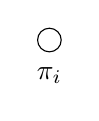
\begin{tikzpicture}
\draw[fill=white] (0,0) circle[radius=0.15];
\draw (0,-0.45) node {$\pi_i$};
\end{tikzpicture}
\end{center}
\item Draw $n_{ij}$ lines between the circles representing the roots $\pi_i$ and $\pi_j$;
\begin{center}
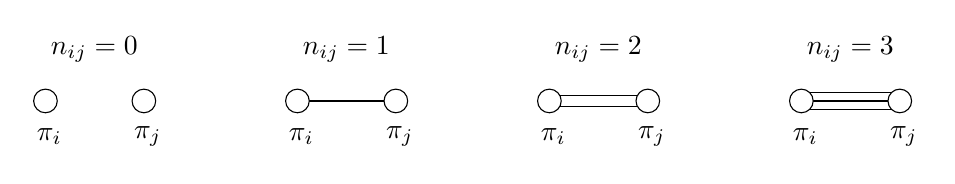
\begin{tikzpicture}
\draw (3.2,0) -- (3.2+1.25,0);
\draw (2*3.2,0.07) -- (2*3.2+1.25,0.07);
\draw (2*3.2,-0.07) -- (2*3.2+1.25,-0.07); 
\draw (3*3.2,0.11) -- (3*3.2+1.25,0.11); 
\draw (3*3.2,0) -- (3*3.2+1.25,0); 
\draw (3*3.2,-0.11) -- (3*3.2+1.25,-0.11); 
\foreach \x in {0,1,2,3} {
\draw (3.2*\x+0.62,0.65) node {$n_{ij}=\x$};
\draw (3.2*\x+0.05,-0.45) node {$\pi_i$};
\draw (3.2*\x+1.3,-0.45) node {$\pi_j$};
\draw[fill=white] (3.2*\x,0) circle[radius=0.15];
\draw[fill=white] (3.2*\x+1.25,0) circle[radius=0.15];
}
\end{tikzpicture}
\end{center}
\item If $n_{ij}=2$ or $3$, draw an arrow on the lines from the longer root to the shorter root.
\begin{center}
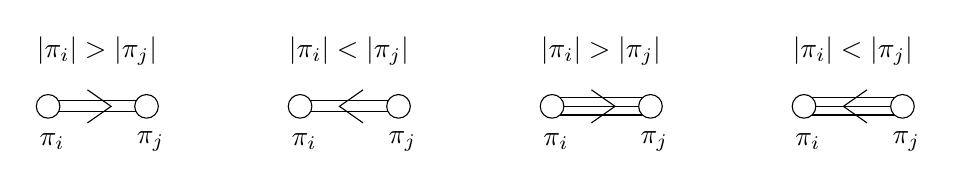
\begin{tikzpicture}
\foreach \x in {0,1} {
\draw (2*3.2*\x+0.62,0.7) node {$|\pi_i|>|\pi_j|$};
\draw (2*3.2*\x+0.65-0.15,0.21) -- (2*3.2*\x+0.65+0.15,0) -- (2*3.2*\x+0.65-0.15,-0.21);
\draw (2*3.2*\x+3.2+0.62,0.7) node {$|\pi_i|<|\pi_j|$};
\draw (2*3.2*\x+3.2+0.65+0.15,0.21) -- (2*3.2*\x+3.2+0.65-0.15,0) -- (2*3.2*\x+3.2+0.65+0.15,-0.21);
\draw (\x*3.2,0.07) -- (\x*3.2+1.25,0.07);
\draw (\x*3.2,-0.07) -- (\x*3.2+1.25,-0.07); 
}
\foreach \x in {2,3} {
\draw (\x*3.2,0.11) -- (\x*3.2+1.25,0.11); 
\draw (\x*3.2,0) -- (\x*3.2+1.25,0); 
\draw (\x*3.2,-0.11) -- (\x*3.2+1.25,-0.11); 
}
\foreach \x in {0,1,2,3} {
\draw (3.2*\x+0.05,-0.45) node {$\pi_i$};
\draw (3.2*\x+1.3,-0.45) node {$\pi_j$};
\draw[fill=white] (3.2*\x,0) circle[radius=0.15];
\draw[fill=white] (3.2*\x+1.25,0) circle[radius=0.15];
}
\end{tikzpicture}
\end{center}
\een
\ed
Dynkin diagrams completely characterise any set of fundamental roots, from which we can reconstruct the entire root set by using the Weyl transformations. The root set can then be used to produce a Cartan-Weyl basis.

We are now finally ready to state the much awaited classification theorem.
\begin{theorem}[Killing, Cartan]\index{Cartan classification}
Any simple finite-dimensional complex Lie algebra can be reconstructed from its set of fundamental roots $\Pi$, which only come in the following forms. 
\ben[label=\roman*)]
\item There are $4$ infinite families
% \bi{rCl}
% A_n & n \geq 1 & 
% \begin{tikzpicture}
% \draw (0,0) edge (2*1.25,0);
% \draw (2*1.25,0) edge[dashed] (3*1.25,0);
% \draw (3*1.25,0) edge (4*1.25,0);
% \foreach \x in {0,1,2,3,4} {
% \draw[fill=white] (1.25*\x,0) circle[radius=0.15];
% }
% \end{tikzpicture}\\
% B_n & n \geq 2 & 
% \begin{tikzpicture}
% \draw (0,0) edge (2*1.25,0);
% \draw (2*1.25,0) edge[dashed] (3*1.25,0);
% \draw (3*1.25+0.65-0.15,0.21) -- (3*1.25+0.65+0.15,0) -- (3*1.25+0.65-0.15,-0.21);
% \draw (3*1.25,0.07) -- (4*1.25,0.07);
% \draw (3*1.25,-0.07) -- (4*1.25,-0.07); 
% \foreach \x in {0,1,2,3,4} {
% \draw[fill=white] (1.25*\x,0) circle[radius=0.15];
% }
% \end{tikzpicture}\\
% C_n & n \geq 3 & 
% \begin{tikzpicture}
% \draw (0,0) edge (2*1.25,0);
% \draw (2*1.25,0) edge[dashed] (3*1.25,0);
% \draw (3*1.25+0.65+0.15,0.21) -- (3*1.25+0.65-0.15,0) -- (3*1.25+0.65+0.15,-0.21);
% \draw (3*1.25,0.07) -- (4*1.25,0.07);
% \draw (3*1.25,-0.07) -- (4*1.25,-0.07); 
% \foreach \x in {0,1,2,3,4} {
% \draw[fill=white] (1.25*\x,0) circle[radius=0.15];
% }
% \end{tikzpicture}\\
% D_n & n \geq 4 & 
% \begin{tikzpicture}
% \draw (0,0) edge (2*1.25,0);
% \draw (2*1.25,0) edge[dashed] (3*1.25,0);
% \draw (3*1.25,0) -- (4*1.25,0.7);
% \draw (3*1.25,0) -- (4*1.25,-0.7); 
% \foreach \x in {0,1,2,3} {
% \draw[fill=white] (1.25*\x,0) circle[radius=0.15];
% }
% \draw[fill=white] (1.25*4,0.7) circle[radius=0.15];
% \draw[fill=white] (1.25*4,-0.7) circle[radius=0.15];
% \end{tikzpicture}
% \ei

\begin{center}
\def\arraystretch{2.5}
\setlength\tabcolsep{15pt}
\begin{tabular}{ccc}
$A_n$ & $n \geq 1$ & 
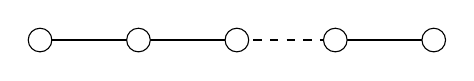
\begin{tikzpicture}[baseline={($ (current bounding box.center) - (0,3pt) $)}]
\draw (0,0) edge (2*1.25,0);
\draw (2*1.25,0) edge[dashed] (3*1.25,0);
\draw (3*1.25,0) edge (4*1.25,0);
\foreach \x in {0,1,2,3,4} {
\draw[fill=white] (1.25*\x,0) circle[radius=0.15];
}
\end{tikzpicture}\\
$B_n$ & $n \geq 2$ & 
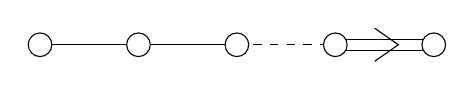
\begin{tikzpicture}[baseline={($ (current bounding box.center) - (0,3pt) $)}]
\draw (0,0) edge (2*1.25,0);
\draw (2*1.25,0) edge[dashed] (3*1.25,0);
\draw (3*1.25+0.65-0.15,0.21) -- (3*1.25+0.65+0.15,0) -- (3*1.25+0.65-0.15,-0.21);
\draw (3*1.25,0.07) -- (4*1.25,0.07);
\draw (3*1.25,-0.07) -- (4*1.25,-0.07); 
\foreach \x in {0,1,2,3,4} {
\draw[fill=white] (1.25*\x,0) circle[radius=0.15];
}
\end{tikzpicture}\\
$C_n$ & $n \geq 3$ & 
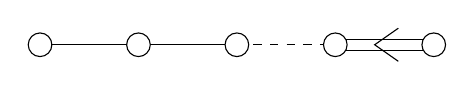
\begin{tikzpicture}[baseline={($ (current bounding box.center) - (0,4pt) $)}]
\draw (0,0) edge (2*1.25,0);
\draw (2*1.25,0) edge[dashed] (3*1.25,0);
\draw (3*1.25+0.65+0.15,0.21) -- (3*1.25+0.65-0.15,0) -- (3*1.25+0.65+0.15,-0.21);
\draw (3*1.25,0.07) -- (4*1.25,0.07);
\draw (3*1.25,-0.07) -- (4*1.25,-0.07); 
\foreach \x in {0,1,2,3,4} {
\draw[fill=white] (1.25*\x,0) circle[radius=0.15];
}
\end{tikzpicture}\\[10pt]
$D_n$ & $n \geq 4$ & 
\begin{tikzpicture}[baseline={($ (current bounding box.center) - (0,3pt) $)}]
\draw (0,0) edge (2*1.25,0);
\draw (2*1.25,0) edge[dashed] (3*1.25,0);
\draw (3*1.25,0) -- (4*1.25,0.7);
\draw (3*1.25,0) -- (4*1.25,-0.7); 
\foreach \x in {0,1,2,3} {
\draw[fill=white] (1.25*\x,0) circle[radius=0.15];
}
\draw[fill=white] (1.25*4,0.7) circle[radius=0.15];
\draw[fill=white] (1.25*4,-0.7) circle[radius=0.15];
\end{tikzpicture}
\end{tabular}
\end{center}
where the restrictions on $n$ ensure that we don't get repeated diagrams (the diagram $D_2$ is excluded since it is disconnected and does not correspond to a simple Lie algebra)

\item five exceptional cases

\begin{center}
\def\arraystretch{2.5}
\setlength\tabcolsep{15pt}
\begin{tabular}{cl}
$E_6$  & 
\begin{tikzpicture}[baseline={($ (current bounding box.south) + (0,1pt) $)}]
\draw (0,0) edge (4*1.25,0);
\draw (2*1.25,0) edge (2*1.25,1.25);
\foreach \x in {0,1,2,3,4} {
\draw[fill=white] (1.25*\x,0) circle[radius=0.15];
}
\draw[fill=white] (2*1.25,1.25) circle[radius=0.15];
\end{tikzpicture}\\[5pt]
$E_7$ & 
\begin{tikzpicture}[baseline={($ (current bounding box.south) + (0,1pt) $)}]
\draw (0,0) edge (5*1.25,0);
\draw (2*1.25,0) edge (2*1.25,1.25);
\foreach \x in {0,1,2,3,4,5} {
\draw[fill=white] (1.25*\x,0) circle[radius=0.15];
}
\draw[fill=white] (2*1.25,1.25) circle[radius=0.15];
\end{tikzpicture}\\[5pt]
$E_8$ &  
\begin{tikzpicture}[baseline={($ (current bounding box.south) + (0,1pt) $)}]
\draw (0,0) edge (6*1.25,0);
\draw (2*1.25,0) edge (2*1.25,1.25);
\foreach \x in {0,1,2,3,4,5,6} {
\draw[fill=white] (1.25*\x,0) circle[radius=0.15];
}
\draw[fill=white] (2*1.25,1.25) circle[radius=0.15];
\end{tikzpicture}\\
$F_4$ & 
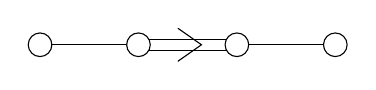
\begin{tikzpicture}[baseline={($ (current bounding box.center) - (0,3pt) $)}]
\draw (0,0) edge (1.25,0);
\draw (2*1.25,0) edge (3*1.25,0);
\draw (1*1.25+0.65-0.15,0.21) -- (1*1.25+0.65+0.15,0) -- (1*1.25+0.65-0.15,-0.21);
\draw (1*1.25,0.07) -- (2*1.25,0.07);
\draw (1*1.25,-0.07) -- (2*1.25,-0.07); 
\foreach \x in {0,1,2,3} {
\draw[fill=white] (1.25*\x,0) circle[radius=0.15];
}
\end{tikzpicture}\\
$G_2$ & 
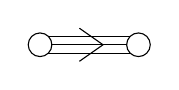
\begin{tikzpicture}[baseline={($ (current bounding box.center) - (0,3pt) $)}]
\draw (0,0) edge (1.25,0);
\draw (0.65-0.15,0.21) -- (0.65+0.15,0) -- (0.65-0.15,-0.21);
\draw (0,0.11) -- (1.25,0.11);
\draw (0,-0.11) -- (1.25,-0.11); 
\foreach \x in {0,1} {
\draw[fill=white] (1.25*\x,0) circle[radius=0.15];
}
\end{tikzpicture}
\end{tabular}
\end{center}
\een
and no other. These are all the possible (connected) Dynkin diagrams.
\end{theorem}

At last, we have achieved a classification of all simple finite-dimensional complex Lie algebras. The finite-dimensional semi-simple complex Lie algebras are direct sums of simple Lie algebras, and correspond to disconnected Dynkin diagrams whose connected components are the ones listed above.













% \newpage

% \section{The Lie group \texorpdfstring{$\SL(2,\C)$}{SL(2,C)} and its Lie algebra \texorpdfstring{$\sl(2,\C)$}{sl(2,C)}}
% 
\subsection{The structure of \texorpdfstring{$\SL(2,\C)$}{SL(2,C)}}

Recall the the Lie group structure is the combination of a number of simpler structures, which we will now examine in detail for the \emph{special linear group} of degree $2$ over $\C$, also known as the \emph{relativistic spin group}\index{relativistic spin group}.

\subsubsection*{$\SL(2,\C)$ as a set}
We define the following subset of $\C^4:=\C\times\C\times\C\times\C$
\bse
\SL(2,\C) := \biggl\{ \biggl(\begin{matrix} a & b \\ c & d\end{matrix}\biggr) \in \C^4 \ \Big|\ ad-bc = 1 \biggr\},
\ese
where the array is just an alternative notation for a quadruple.

\subsubsection*{$\SL(2,\C)$ as a group}

We define an operation
\bi{rrCl}
\bullet \cl & \SL(2,\C) \times \SL(2,\C) & \to & \SL(2,\C)\\[3pt]
& (\biggl(\begin{matrix} a & b \\ c & d\end{matrix}\biggr) ,\biggl(\begin{matrix} e & f \\ g & h\end{matrix}\biggr))  & \mapsto & \biggl(\begin{matrix} a & b \\ c & d\end{matrix}\biggr) \bullet \biggl(\begin{matrix} e & f \\ g & h\end{matrix}\biggr),
\ei
where
\bse
\biggl(\begin{matrix} a & b \\ c & d\end{matrix}\biggr) \bullet \biggl(\begin{matrix} e & f \\ g & h\end{matrix}\biggr) := \biggl(\begin{matrix} ae+bg & af+bh \\ ce+dg & cf+dh\end{matrix}\biggr).
\ese
Formally, this operation is the same as matrix multiplication. We can check directly that the result of applying $\bullet$ lands back in $\SL(2,\C)$, or simply recall that the determinant of a product is the product of the determinants. Moreover, the operation $\bullet$
\ben[label=\roman*)]
\item is associative (straightforward but tedious to check);
\item has an identity element, namely $\biggl(\begin{matrix} 1 & 0 \\ 0 & 1\end{matrix}\biggr)\in \SL(2,\C)$;
\item admits inverses: for each $\biggl(\begin{matrix} a & b \\ c & d\end{matrix}\biggr)\in \SL(2,\C)$, we have $\biggl(\begin{matrix} d & -b \\ -c & a\end{matrix}\biggr)\in \SL(2,\C)$ and
\bse
\biggl(\begin{matrix} a & b \\ c & d\end{matrix}\biggr)\bullet\biggl(\begin{matrix} d & -b \\ -c & a\end{matrix}\biggr) = \biggl(\begin{matrix} d & -b \\ -c & a\end{matrix}\biggr)\bullet \biggl(\begin{matrix} a & b \\ c & d\end{matrix}\biggr) = \biggl(\begin{matrix} 1 & 0 \\ 0 & 1\end{matrix}\biggr).
\ese
Hence, we have $\biggl(\begin{matrix} a & b \\ c & d\end{matrix}\biggr)^{-1}= \biggl(\begin{matrix} d & -b \\ -c & a\end{matrix}\biggr)$.
\een
Therefore, the pair $(\SL(2,\C),\bullet)$ is a (non-commutative) group.

\subsubsection*{$\SL(2,\C)$ as a topological space}

Recall that if $N$ is a subset of $M$ and $\mathcal{O}$ is a topology on $M$, then we can equip $N$ with the subset topology inherited from $M$
\bse
\mathcal{O}|_N := \{U\cap N \mid U \in \mathcal{O}\}.
\ese
We begin by establishing a topology on $\C$ as follows. Let
\bse
B_r(z):=\{y\in\C\mid |z-y|<r\}
\ese
be the open ball of radius $r>0$ and centre $z\in \C$.
\begin{center}
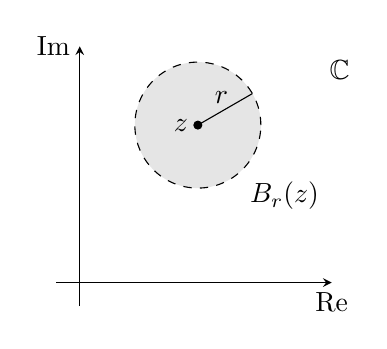
\begin{tikzpicture}
\draw [->] (-0.3,0) -- (3.2,0) node[below] {Re}; 
\draw [->] (0,-0.3) -- (0,3) node[left] {Im}; 
\draw[fill=lightergray,dashed]  (1.5,2) circle (0.8) node[left] {$z$};
\draw (1.8,2.35) node {$r$};
\draw[fill]  (1.5,2) circle (0.05);
\draw (1.5,2) edge +(0.8*cos 30,0.8*sin 30);
\draw (3.3,2.7) node {$\C$};
\draw (2.6,1.1) node {$B_r(z)$};
\end{tikzpicture}
\end{center}
Define $\mathcal{O}_\C$ implicitly by
\bse
U\in \mathcal{O}_\C\ :\Leftrightarrow\ \forall \, z \in U : \exists \, r>0 : B_r(z)\se U.
\ese
Then, the pair $(\C,\mathcal{O}_\C)$ is a topological space. In fact, we have
\bse
(\C,\mathcal{O}_\C) \cong_\mathrm{top} (\R^2,\mathcal{O}_\mathrm{std}).
\ese
We can then equip $\C^4$ with the product topology so that we can finally define
\bse
\mathcal{O} := (\mathcal{O}_\C)|_{\SL(2,\C)},
\ese
so that the pair $(\SL(2,\C),\mathcal{O})$ is a topological space. In fact, it is a connected topological space, and we will need this property later on.

\subsubsection*{$\SL(2,\C)$ as a topological manifold}

Recall that a topological space $(M,\mathcal{O})$ is a complex topological manifold if each point $p\in M$ has an open neighbourhood $U(p)$ which is homeomorphic to an open subset of $\C^d$. Equivalently, there must exist a $\mathcal{C}^0$-atlas, i.e.\ a collection $\mathscr{A}$ of charts $(U_\alpha,x_\alpha)$, where the $U_\alpha$ are open and cover $M$ and each $x$ is a homeomorphism onto a subset of $\C^d$.

Let $U$ be the set
\bse
U:= \biggl\{ \biggl( \begin{matrix} a & b \\ c & d \end{matrix}\biggr) \in \SL(2,\C) \ \Big| \ a \neq 0 \biggr\}
\ese
and define the map
\bi{rrCl}
x \cl & U & \to & x(U) \se \C^*\times\C\times \C\\
& \biggl( \begin{matrix} a & b \\ c & d \end{matrix}\biggr) & \mapsto & (a,b,c),
\ei
where $\C^*=\C\setminus\{0\}$. With a little work, one can show that $U$ is an open subset of $(\SL(2,\C),\mathcal{O})$ and $x$ is a homeomorphism with inverse
\bi{rrCl}
x^{-1} \cl & x(U) & \to & U\\
& (a,b,c)& \mapsto & \biggl( \begin{matrix} a & b \\ c & \frac{1+bc}{a} \end{matrix}\biggr) .
\ei
However, since $\SL(2,\C)$ contains elements with $a=0$, the chart $(U,x)$ does not cover the whole space, and hence we need at least one more chart. We thus define the set
\bse
V:= \biggl\{ \biggl( \begin{matrix} a & b \\ c & d \end{matrix}\biggr) \in \SL(2,\C) \ \Big| \ b \neq 0 \biggr\}
\ese
and the map
\bi{rrCl}
y \cl & V & \to & x(V) \se \C\times \C^*\times \C\\
& \biggl( \begin{matrix} a & b \\ c & d \end{matrix}\biggr) & \mapsto & (a,b,d).
\ei
Similarly to the above, $V$ is open and $y$ is a homeomorphism with inverse
\bi{rrCl}
y^{-1} \cl & x(V) & \to & V\\
& (a,b,d)& \mapsto & \biggl( \begin{matrix} a & b \\ \frac{ad-1}{b}  & d\end{matrix}\biggr) .
\ei
An element of $\SL(2,\C)$ cannot have both $a$ and $b$ equal to zero, for otherwise $ad-bc=0\neq 1$. Hence $\mathscr{A}_{\mathrm{top}}:=\{(U,x),(V,y)\}$ is an atlas, and since every atlas is automatically a $\mathcal{C}^0$-atlas, the triple $(\SL(2,\C),\mathcal{O},\mathscr{A}_{\mathrm{top}})$ is a 3-dimensional, complex, topological manifold.

\subsubsection*{$\SL(2,\C)$ as a complex differentiable manifold}

Recall that to obtain a $\mathcal{C}^1$-differentiable manifold from a topological manifold with atlas $\mathscr{A}$, we have to check that every transition map between charts in $\mathscr{A}$ is differentiable in the usual sense.

In our case, we have the atlas $\mathscr{A}_{\mathrm{top}}:=\{(U,x),(V,y)\}$. We evaluate
\bse
(y\circ x^{-1})(a,b,c) = y (\biggl( \begin{matrix} a & b \\ c & \frac{1+bc}{a} \end{matrix}\biggr) ) = (a,b,\tfrac{1+bc}{a}).
\ese
Hence we have the transition map 
\bi{rrCl}
y\circ x^{-1} \cl & x(U\cap V) & \to & y(U\cap V)\\
& (a,b,c) & \mapsto & ( a,b,\tfrac{1+bc}{a}).
\ei
Similarly, we have 
\bse
(x\circ y^{-1})(a,b,d) = y (\biggl( \begin{matrix} a & b \\ \frac{ad-1}{b} & d \end{matrix}\biggr) ) = (a,b,\tfrac{ad-1}{b}).
\ese
Hence, the other transition map is 
\bi{rrCl}
x\circ y^{-1} \cl & y(U\cap V) & \to & x(U\cap V)\\
& (a,b,c) & \mapsto & ( a,b,\tfrac{ad-1}{b}).
\ei
Since $a\neq 0$ and $b\neq 0$, the transition maps are complex differentiable (this is a good time to review your complex analysis!). 

Therefore, the atlas $\mathscr{A}_{\mathrm{top}}$ is a differentiable atlas. By defining $\mathscr{A}$ to be the maximal differentiable atlas containing $\mathscr{A}_{\mathrm{top}}$, we have that $(\SL(2,\C),\mathcal{O},\mathscr{A})$ is a 3-dimensional, complex differentiable manifold.

\subsubsection*{$\SL(2,\C)$ as a Lie group}

We equipped $\SL(2,\C)$ with both a group and a manifold structure. In order to obtain a Lie group structure, we have to check that these two structures are compatible, that is, we have to show that the two maps
\bi{rrCl}
\mu \cl & \SL(2,\C) \times \SL(2,\C) & \to & \SL(2,\C)\\[3pt]
& (\biggl(\begin{matrix} a & b \\ c & d\end{matrix}\biggr) ,\biggl(\begin{matrix} e & f \\ g & h\end{matrix}\biggr))  & \mapsto & \biggl(\begin{matrix} a & b \\ c & d\end{matrix}\biggr) \bullet \biggl(\begin{matrix} e & f \\ g & h\end{matrix}\biggr)
\ei
and 
\bi{rrCl}
i \cl & \SL(2,\C) & \to & \SL(2,\C)\\[3pt]
& \biggl(\begin{matrix} a & b \\ c & d\end{matrix}\biggr)  & \mapsto &\biggl(\begin{matrix} a & b \\ c & d\end{matrix}\biggr)^{-1} %= \biggl(\begin{matrix} d & -b \\ -c & a\end{matrix}\biggr)
\ei
are differentiable with respect to the differentiable structure on $\SL(2,\C)$. For instance, for the inverse map $i$, we have to show that the map $y\circ i \circ x^{-1}$ is differentiable in the usual for any pair of charts $(U,x),(V,y)\in \mathscr{A}$. 
\bse
\begin{tikzcd}
U \se\SL(2,\C) \ar[dd,"x"]\ar[rr,"i"]&& V\se \SL(2,\C)\ar[dd,"y"]\\
&&\\
x(U) \se \C^3 \ar[rr,"y\circ i\circ x^{-1}"]&& y(V)\se \C^3
\end{tikzcd}
\ese
However, since $\SL(2,\C)$ is connected, the differentiability of the transition maps in $\mathscr{A}$ implies that if $y\circ i\circ x^{-1}$ is differentiable for any two given charts, then it is differentiable for all charts in $\mathscr{A}$. Hence, we can simply let $(U,x)$ and $(V,y)$ be the two charts on $\SL(2,\C)$ defined above. Then, we have
\bse
(y\circ i\circ x^{-1}) (a,b,c) = (y\circ i) ( \biggl(\begin{matrix} a & b \\ c & \frac{1+bc}{a}\end{matrix}\biggr) ) = y ( \biggl(\begin{matrix} \frac{1+bc}{a} & -b \\ -c & a\end{matrix}\biggr)) = (\tfrac{1+bc}{a},-b,a)
\ese
which is certainly complex differentiable as a map between open subsets of $\C^3$ (recall that $a\neq 0$ on $x(U)$).

Checking that $\mu$ is complex differentiable is slightly more involved, since we first have to equip $\SL(2,\C) \times \SL(2,\C)$ with a suitable ``product differentiable structure'' and then proceed as above. Once that is done, we can finally conclude that $((\SL(2,\C),\mathcal{O},\mathscr{A}),\bullet)$ is a $3$-dimensional complex Lie group.

\subsection{The Lie algebra of \texorpdfstring{$\SL(2,\C)$}{SL(2,C)}}

Recall that to every Lie group $G$, there is an associated Lie algebra $\mathcal{L}(G)$, where
\bse
\mathcal{L}(G) := \{X\in \Gamma(TG)\mid \forall \, g,h\in G : (\ell_g)_*(X|_h)=X_{gh}\},
\ese
which we then proved to be isomorphic to the Lie algebra $T_eG$ with Lie bracket
\bse
[A,B]_{T_eG} := j^{-1} ([j(A),j(B)]_{\mathcal{L}(G)})
\ese
induced by the Lie bracket on $\mathcal{L}(G)$ via the isomorphism $j$
\bse
j(A)|_g := (\ell_g)_*(A).
\ese
In the case of $\SL(2,\C)$, the left translation map by $\left(\begin{smallmatrix}a & b \\ c & d\end{smallmatrix}\right)$ is 
\bi{rrCl}
\ell_{\left(\begin{smallmatrix}a & b \\ c & d\end{smallmatrix}\right)} \cl & \SL(2,\C) &\to & \SL(2,\C)\\
& \biggl(\begin{matrix}e & f \\ g  & h\end{matrix}\biggr) & \mapsto & \biggl(\begin{matrix}a & b \\ c & d\end{matrix}\biggr) \bullet \biggl(\begin{matrix}e & f \\ g  & h\end{matrix}\biggr) 
\ei
By using the standard notation $\sl(2,\C)\equiv \mathcal{L}(\SL(2,\C))$, we have
\bse
\sl(2,\C) \cong_{\mathrm{Lie \, alg}} T_{\left(\begin{smallmatrix}1 & 0 \\ 0 & 1\end{smallmatrix}\right)}\SL(2,\C).
\ese
We would now like to explicitly determine the Lie bracket on $T_{\left(\begin{smallmatrix}1 & 0 \\ 0 & 1\end{smallmatrix}\right)}\SL(2,\C)$, and hence determine its structure constants.

Recall that if $(U,x)$ is a chart on a manifold $M$ and $p\in U$, then the chart $(U,x)$ induces a basis of the tangent space $T_pM$. We shall use our previously defined chart $(U,x)$ on $\SL(2,\C)$, where $U:= \{ \left( \begin{smallmatrix} a & b \\ c & d \end{smallmatrix}\right) \in \SL(2,\C) \mid a \neq 0 \}$ and 
\bi{rrCl}
x \cl & U & \to & x(U) \se \C^3\\
& \biggl( \begin{matrix} a & b \\ c & d \end{matrix}\biggr) & \mapsto & (a,b,c).
\ei
Note that the $d$ appearing here is completely redundant, since the membership condition of $\SL(2,\C)$ forces $d=\frac{1+bc}{a}$. However, we will keep writing the $d$ to avoid having a fraction in a matrix in a subscript.

The chart $(U,x)$ contains $\left(\begin{smallmatrix}1 & 0 \\ 0 & 1\end{smallmatrix}\right)$ and hence we get an induced co-ordinate basis
\bse
\biggl\{\tvb{x}{i}{\left(\begin{smallmatrix}1 & 0 \\ 0 & 1\end{smallmatrix}\right)}\in  T_{\left(\begin{smallmatrix}1 & 0 \\ 0 & 1\end{smallmatrix}\right)}\SL(2,\C) \ \Big| \ 1\leq i \leq 3 \biggr\}
\ese
so that any $A\in  T_{\left(\begin{smallmatrix}1 & 0 \\ 0 & 1\end{smallmatrix}\right)}\SL(2,\C)$ can be written as
\bse
A = \lambda^1 \tvb{x}{1}{\left(\begin{smallmatrix}1 & 0 \\ 0 & 1\end{smallmatrix}\right)} + \lambda^2 \tvb{x}{2}{\left(\begin{smallmatrix}1 & 0 \\ 0 & 1\end{smallmatrix}\right)} + \lambda^3\tvb{x}{3}{\left(\begin{smallmatrix}1 & 0 \\ 0 & 1\end{smallmatrix}\right)},
\ese
for some $\lambda^1, \lambda^2,\lambda^3\in \C$. Since the Lie bracket is bilinear, its action on these basis vectors uniquely extends to the whole of $T_{\left(\begin{smallmatrix}1 & 0 \\ 0 & 1\end{smallmatrix}\right)}\SL(2,\C)$ by linear continuation. Hence, we simply have to determine the action of the Lie bracket of $\sl(2,\C)$ on the images under the isomorphism $j$ of these basis vectors. 

Let us now determine the image of these co-ordinate induced basis elements under the isomorphism $j$. The object
\bse
j\biggl(    \tvb{x}{i}{\left(\begin{smallmatrix}1 & 0 \\ 0 & 1\end{smallmatrix}\right)}\biggr) \in \sl(2,\C) 
\ese
is a left-invariant vector field on $\SL(2,\C)$. It assigns to each point $\left(\begin{smallmatrix}a & b \\ c & d\end{smallmatrix}\right)\in U\se \SL(2,\C)$ the tangent vector
\bse
j\biggl(    \tvb{x}{i}{\left(\begin{smallmatrix}1 & 0 \\ 0 & 1\end{smallmatrix}\right)}\biggr) \bigg|_{\left(\begin{smallmatrix}a & b \\ c & d\end{smallmatrix}\right)} : =
\Bigl(\ell_{\left(\begin{smallmatrix}a & b \\ c & d\end{smallmatrix}\right)} \Bigr)_*     \tvb{x}{i}{\left(\begin{smallmatrix}1 & 0 \\ 0 & 1\end{smallmatrix}\right)} \in T_{\left(\begin{smallmatrix}a & b \\ c & d\end{smallmatrix}\right)}\SL(2,\C). 
\ese
This tangent vector is a $\C$-linear map $\mathcal{C}^\infty(\SL(2,\C))\xrightarrow{\sim}\C$, where $\mathcal{C}^\infty(\SL(2,\C))$ is the $\C$-vector space (in fact, the $\C$-algebra) of smooth complex-valued functions on $\SL(2,\C)$ although, to be precise, since we are working in a chart we should only consider functions defined on $U$. For (the restriction to $U$ of) any $f\in \mathcal{C}^\infty(\SL(2,\C))$ we have, explicitly,
\bi{rCl}
\Bigl(\ell_{\left(\begin{smallmatrix}a & b \\ c & d\end{smallmatrix}\right)} \Bigr)_*     \tvb{x}{i}{\left(\begin{smallmatrix}1 & 0 \\ 0 & 1\end{smallmatrix}\right)} (f) & = & \tvb{x}{i}{\left(\begin{smallmatrix}1 & 0 \\ 0 & 1\end{smallmatrix}\right)} \Bigl(f\circ \ell_{\left(\begin{smallmatrix}a & b \\ c & d\end{smallmatrix}\right)} \Bigr)\\
& = & \partial_i\Bigl(f\circ \ell_{\left(\begin{smallmatrix}a & b \\ c & d\end{smallmatrix}\right)} \circ x^{-1}\Bigr) (x\left(\begin{smallmatrix}1 & 0 \\ 0 & 1\end{smallmatrix}\right)),
\ei
where the argument of $\partial_i$ in the last line is a map $x(U)\se\C^3\to\C$, hence $\partial_i$ is simply the operation of complex differentiation with respect to the $i$-th (out of the 3) complex variable of the map $f\circ \ell_{\left(\begin{smallmatrix}a & b \\ c & d\end{smallmatrix}\right)} \circ x^{-1}$, which is then to be evaluated at $x\left(\begin{smallmatrix}1 & 0 \\ 0 & 1\end{smallmatrix}\right)\in \C^3$. By inserting an identity in the composition, we have
\bi{rCl}
& = &\partial_i\Bigl(f\circ {\id_U} \circ \ell_{\left(\begin{smallmatrix}a & b \\ c & d\end{smallmatrix}\right)} \circ x^{-1}\Bigr) (x\left(\begin{smallmatrix}1 & 0 \\ 0 & 1\end{smallmatrix}\right)) \\
& = & \partial_i\Bigl(f\circ ( x^{-1}\circ x) \circ \ell_{\left(\begin{smallmatrix}a & b \\ c & d\end{smallmatrix}\right)} \circ x^{-1}\Bigr) (x\left(\begin{smallmatrix}1 & 0 \\ 0 & 1\end{smallmatrix}\right))\\
& = & \partial_i\Bigl((f\circ  x^{-1})\circ (x \circ \ell_{\left(\begin{smallmatrix}a & b \\ c & d\end{smallmatrix}\right)} \circ x^{-1})\Bigr) (x\left(\begin{smallmatrix}1 & 0 \\ 0 & 1\end{smallmatrix}\right)),
\ei
where $f\circ  x^{-1}\cl x(U)\se \C^3 \to \C$ and $(x \circ \ell_{\left(\begin{smallmatrix}a & b \\ c & d\end{smallmatrix}\right)} \circ x^{-1})\cl x(U)\se \C^3 \to x(U)\se\C^3$ and hence, we can use the multi-dimensional chain rule to obtain
\bi{rCl}
& = & \Bigl(\partial_m(f\circ  x^{-1})\bigl((x \circ \ell_{\left(\begin{smallmatrix}a & b \\ c & d\end{smallmatrix}\right)} \circ x^{-1}) (x\left(\begin{smallmatrix}1 & 0 \\ 0 & 1\end{smallmatrix}\right))\bigr)\Bigr)\Bigl( 
\partial_i (x^m \circ \ell_{\left(\begin{smallmatrix}a & b \\ c & d\end{smallmatrix}\right)} \circ x^{-1}) (x\left(\begin{smallmatrix}1 & 0 \\ 0 & 1\end{smallmatrix}\right))\Bigr),
\ei
with the summation going from $m=1$ to $m=3$. The first factor is simply
\bi{rCl}
\partial_m(f\circ  x^{-1})\bigl((x \circ \ell_{\left(\begin{smallmatrix}a & b \\ c & d\end{smallmatrix}\right)}) \left(\begin{smallmatrix}1 & 0 \\ 0 & 1\end{smallmatrix}\right)\bigr) & =\phantom{:} & \partial_m(f\circ  x^{-1})(x\left(\begin{smallmatrix}a & b \\ c & d\end{smallmatrix}\right))\\
& =: & \tvb{x}{m}{\left(\begin{smallmatrix}a & b \\ c & d\end{smallmatrix}\right)} (f) .
\ei
To see what the second factor is, we first consider the map $x^m \circ \ell_{\left(\begin{smallmatrix}a & b \\ c & d\end{smallmatrix}\right)} \circ x^{-1}$. This map acts on the triple $(e,f,g)\in x(U)$ as
\bi{rCl}
(x^m \circ \ell_{\left(\begin{smallmatrix}a & b \\ c & d\end{smallmatrix}\right)} \circ x^{-1}) (e,f,g) & = & (x^m \circ \ell_{\left(\begin{smallmatrix}a & b \\ c & d\end{smallmatrix}\right)} ) \biggl(\begin{matrix}e & f \\ g & \frac{1+fg}{e}\end{matrix}\biggr)\\
& = & x^m (\biggl(\begin{matrix}a & b \\ c & d\end{matrix}\biggr) \bullet \biggl(\begin{matrix}e & f \\ g & \frac{1+fg}{e}\end{matrix}\biggr))\\
& = & x^m (\left(\begin{matrix}ae+bg &\, af+ \frac{b(1+fg)}{e} \\ ce+dg &\, cf+\frac{d(1+fg)}{e}\end{matrix}\right) ),
\ei
and since $x^m := {\proj_m} \circ x$, with $m\in \{1,2,3\}$, we have 
\bse
(x^m \circ \ell_{\left(\begin{smallmatrix}a & b \\ c & d\end{smallmatrix}\right)} \circ x^{-1}) (e,f,g) = \proj_m (ae+bg, af+ \tfrac{b(1+fg)}{e}, ce+dg ),
\ese
the map $\proj_m$ simply picks the $m$-th component of the triple. We now have to apply $\partial_i$ to this map, with $i\in \{1,2,3\}$, i.e.\ we have to differentiate with respect to each of the three complex variables $e$, $f$, and $g$. We can write the result as
\bse
\partial_i(x^m \circ \ell_{\left(\begin{smallmatrix}a & b \\ c & d\end{smallmatrix}\right)} \circ x^{-1}) (e,f,g)= D(e,f,g)^m_{\phantom{m}i},
\ese
where $m$ labels the rows and $i$ the columns of the matrix
\bse
D(e,f,g)= \left(\begin{matrix}a & 0 & b\\ -\frac{b(1+fg)}{e^2} &\,a+\frac{bg}{e} &\frac{bf}{e}\\ c & 0 & d\end{matrix}\right).
\ese
Finally, by evaluating this at $(e,f,g)=x\left(\begin{smallmatrix}1 & 0 \\ 0 & 1\end{smallmatrix}\right) = (1,0,0)$, we obtain
\bse
\partial_i(x^m \circ \ell_{\left(\begin{smallmatrix}a & b \\ c & d\end{smallmatrix}\right)} \circ x^{-1}) (x\left(\begin{smallmatrix}1 & 0 \\ 0 & 1\end{smallmatrix}\right))= D^m_{\phantom{m}i},
\ese
where, by recalling that $d=\frac{1+bc}{a}$,
\bse
D:= D(1,0,0)= \left(\begin{matrix}a & 0 & b\ \\ -b & a & 0\\ c & 0 & \frac{1+bc}{a}\end{matrix}\right).
\ese
Putting the two factors back together yields
\bse
\Bigl(\ell_{\left(\begin{smallmatrix}a & b \\ c & d\end{smallmatrix}\right)} \Bigr)_*     \tvb{x}{i}{\left(\begin{smallmatrix}1 & 0 \\ 0 & 1\end{smallmatrix}\right)} (f) =  D^m_{\phantom{m}i} \tvb{x}{m}{\left(\begin{smallmatrix}a & b \\ c & d\end{smallmatrix}\right)} (f) .
\ese
Since this holds for an arbitrary $f\in\mathcal{C}^\infty(\SL(2,\C))$, we have
\bse
j\biggl(    \tvb{x}{i}{\left(\begin{smallmatrix}1 & 0 \\ 0 & 1\end{smallmatrix}\right)}\biggr) \bigg|_{\left(\begin{smallmatrix}a & b \\ c & d\end{smallmatrix}\right)} : =
\Bigl(\ell_{\left(\begin{smallmatrix}a & b \\ c & d\end{smallmatrix}\right)} \Bigr)_*     \tvb{x}{i}{\left(\begin{smallmatrix}1 & 0 \\ 0 & 1\end{smallmatrix}\right)} = D^m_{\phantom{m}i} \tvb{x}{m}{\left(\begin{smallmatrix}a & b \\ c & d\end{smallmatrix}\right)}, 
\ese
and since the point $\left(\begin{smallmatrix}a & b \\ c & d\end{smallmatrix}\right)\in U\se\SL(2,\C)$ is also arbitrary, we have
\bse
j\biggl( \tvb{x}{i}{\left(\begin{smallmatrix}1 & 0 \\ 0 & 1\end{smallmatrix}\right)}\biggr) = D^m_{\phantom{m}i}\, \frac{\partial}{\partial x^m} \in \sl(2,\C),
\ese
where $D$ is now the corresponding matrix of co-ordinate functions
\bse
D:=\left(\begin{matrix}x^1 & 0 & x^2\ \\ -x^2 & x^1 & 0\\ x^3 & 0 & \frac{1+x^2x^3}{x^1}\end{matrix}\right).
\ese
Note that while the three vector fields
\bi{rrCl}
\frac{\partial}{\partial x^m} \cl &  \SL(2,\C) & \to &  T\SL(2,\C)\\
& \biggl(\begin{matrix}a & b \\ c & d\end{matrix}\biggr) & \mapsto & \tvb{x}{m}{\left(\begin{smallmatrix}a & b \\ c & d\end{smallmatrix}\right)}
\ei
are not individually left-invariant, their linear combination with coefficients $D^m_{\phantom{m}i}$ is indeed left-invariant. Recall that these vector fields
\ben[label=\roman*)]
\item are $\C$-linear maps
\bi{rrCl}
\frac{\partial}{\partial x^m}\cl &\mathcal{C}^\infty(\SL(2,\C))&\xrightarrow{\sim} &\mathcal{C}^\infty(\SL(2,\C))\\
& f & \mapsto & \partial_m(f\circ x^{-1})\circ x;
\ei
\item satisfy the Leibniz rule
\bse
\frac{\partial}{\partial x^m} (fg) = f\frac{\partial}{\partial x^m}(g)+g\frac{\partial}{\partial x^m}(f);
\ese
\item act on the coordinate functions $x^i\in \mathcal{C}^\infty(\SL(2,\C))$ as
\bse
\frac{\partial}{\partial x^m} (x^i) = \partial_m (x^i \circ x^{-1})\circ x = \partial_m ({\proj_i}\circ x \circ x^{-1}) \circ x =\delta^i_m\circ x= \delta^i_m,
\ese
since the composition of a constant function with any composable function is just the constant function.
\een
We now have an expansion of the images of the basis of $T_{\left(\begin{smallmatrix}1 & 0 \\ 0 & 1\end{smallmatrix}\right)}\SL(2,\C)$ under $j$:
\bi{rCl}
j\biggl( \tvb{x}{1}{\left(\begin{smallmatrix}1 & 0 \\ 0 & 1\end{smallmatrix}\right)}\biggr) & = & x^1  \frac{\partial}{\partial x^1} - x^2\frac{\partial}{\partial x^2}  + x^3\frac{\partial}{\partial x^3} \\
j\biggl( \tvb{x}{2}{\left(\begin{smallmatrix}1 & 0 \\ 0 & 1\end{smallmatrix}\right)}\biggr) & = & x^1 \frac{\partial}{\partial x^2}  \\
j\biggl( \tvb{x}{3}{\left(\begin{smallmatrix}1 & 0 \\ 0 & 1\end{smallmatrix}\right)}\biggr) & = & x^2\, \frac{\partial}{\partial x^1} + \tfrac{1+x^2x^3}{x^1} \frac{\partial}{\partial x^3}  .
\ei
We now have to calculate the (vector field) bracket of every pair of these. We can also do them all at once, which is a good exercise in index gymnastics. We have
\bse
\biggl[j\biggl( \tvb{x}{i}{\left(\begin{smallmatrix}1 & 0 \\ 0 & 1\end{smallmatrix}\right)}\biggr) ,j\biggl( \tvb{x}{k}{\left(\begin{smallmatrix}1 & 0 \\ 0 & 1\end{smallmatrix}\right)}\biggr) \biggr] =  \left[  D^m_{\phantom{m}i}\, \frac{\partial}{\partial x^m}, D^n_{\phantom{n}k}\, \frac{\partial}{\partial x^n}\right].
\ese
Letting this act on an arbitrary $f\in \mathcal{C}^\infty(\SL(2,\C))$, by definition
\bse
\left[  D^m_{\phantom{m}i}\, \frac{\partial}{\partial x^m}, D^n_{\phantom{n}k}\, \frac{\partial}{\partial x^n}\right](f) :=  D^m_{\phantom{m}i}\, \frac{\partial}{\partial x^m} \Bigl( D^n_{\phantom{n}k}\, \frac{\partial}{\partial x^n} (f)\Bigr) -  D^n_{\phantom{n}k}\, \frac{\partial}{\partial x^n} \Bigl(D^m_{\phantom{m}i}\, \frac{\partial}{\partial x^m}(f)\Bigr).
\ese
The first term gives
\bi{rCl}
 D^m_{\phantom{m}i}\, \frac{\partial}{\partial x^m} \Bigl( D^n_{\phantom{n}k}\, \frac{\partial}{\partial x^n} (f)\Bigr) & = &  D^m_{\phantom{m}i}\, \frac{\partial}{\partial x^m} ( D^n_{\phantom{n}k}\, \partial_n (f\circ x^{-1})\circ x)\\
& = & D^m_{\phantom{m}i}\, \frac{\partial}{\partial x^m} (D^n_{\phantom{n}k})\,(\partial_n (f\circ x^{-1})\circ x) +  D^m_{\phantom{m}i}D^n_{\phantom{n}k} \,\frac{\partial}{\partial x^m} (\partial_n (f\circ x^{-1})\circ x)\\
& = & D^m_{\phantom{m}i}\, \frac{\partial}{\partial x^m} (D^n_{\phantom{n}k})\,(\partial_n (f\circ x^{-1})\circ x) +  D^m_{\phantom{m}i}D^n_{\phantom{n}k} \,\partial_m(\partial_n (f\circ x^{-1})\circ x\circ x^{-1})\circ x\\
& = & D^m_{\phantom{m}i}\, \frac{\partial}{\partial x^m} (D^n_{\phantom{n}k})\,(\partial_n (f\circ x^{-1})\circ x) +  D^m_{\phantom{m}i}D^n_{\phantom{n}k} \,\partial_m\partial_n (f\circ x^{-1})\circ x.
\ei
Similarly, we have
\bse
D^n_{\phantom{n}k}\, \frac{\partial}{\partial x^n} \Bigl(  D^m_{\phantom{m}i}\, \frac{\partial}{\partial x^m} (f)\Bigr) = D^n_{\phantom{n}k}\, \frac{\partial}{\partial x^n} (D^m_{\phantom{m}i})\,(\partial_m (f\circ x^{-1})\circ x) +  D^n_{\phantom{n}k}D^m_{\phantom{m}i}\,\partial_n\partial_m (f\circ x^{-1})\circ x.
\ese
Hence, recalling that $\partial_m\partial_n=\partial_n\partial_m$ by Schwarz's theorem, we have  
\bi{rCl}
\left[  D^m_{\phantom{m}i}\, \frac{\partial}{\partial x^m}, D^n_{\phantom{n}k}\, \frac{\partial}{\partial x^n}\right](f) &=&  D^m_{\phantom{m}i}\, \frac{\partial}{\partial x^m} (D^n_{\phantom{n}k})\, (\partial_n (f\circ x^{-1})\circ x) +  \Ccancel[gray]{D^m_{\phantom{m}i}D^n_{\phantom{n}k} \,\partial_m\partial_n (f\circ x^{-1})\circ x}\\
& & \negmedspace {} - D^n_{\phantom{n}k}\, \frac{\partial}{\partial x^n} (D^m_{\phantom{m}i})\,(\partial_m (f\circ x^{-1})\circ x) - \Ccancel[gray]{D^n_{\phantom{n}k}D^m_{\phantom{m}i}\,\partial_n\partial_m (f\circ x^{-1})\circ x}\\
& = & \Bigl( D^m_{\phantom{m}i}\, \frac{\partial}{\partial x^m} (D^n_{\phantom{n}k}) - D^m_{\phantom{m}k}\, \frac{\partial}{\partial x^m} (D^n_{\phantom{n}i})\Bigr)\partial_n (f\circ x^{-1})\circ x\\
& = & \Bigl( D^m_{\phantom{m}i}\, \frac{\partial}{\partial x^m} (D^n_{\phantom{n}k}) - D^m_{\phantom{m}k}\, \frac{\partial}{\partial x^m} (D^n_{\phantom{n}i})\Bigr)\frac{\partial}{\partial x^n} (f),
\ei
where we relabelled some dummy indices. Since the $f\in\mathcal{C}^\infty(\SL(2,\C))$ was arbitrary,
\bse
\left[  D^m_{\phantom{m}i}\, \frac{\partial}{\partial x^m}, D^n_{\phantom{n}k}\, \frac{\partial}{\partial x^n}\right] =  \Bigl( D^m_{\phantom{m}i}\, \frac{\partial}{\partial x^m} (D^n_{\phantom{n}k}) - D^m_{\phantom{m}k}\, \frac{\partial}{\partial x^m} (D^n_{\phantom{n}i})\Bigr)\frac{\partial}{\partial x^n} .
\ese
We can now evaluate this explicitly. For $i=1$ and $k=2$, we have
\bi{rCl}
\left[  D^m_{\phantom{m}1} \frac{\partial}{\partial x^m}, D^n_{\phantom{n}2} \frac{\partial}{\partial x^n}\right] &=&  \Bigl( \Ccancel[gray]{D^m_{\phantom{m}1} \frac{\partial}{\partial x^m} (D^1_{\phantom{1}2})} - D^m_{\phantom{m}2} \frac{\partial}{\partial x^m} (D^1_{\phantom{1}1})\Bigr)\frac{\partial}{\partial x^1}\\
& &\negmedspace{}+  \Bigl( D^m_{\phantom{m}1} \frac{\partial}{\partial x^m} (D^2_{\phantom{2}2}) - D^m_{\phantom{m}2} \frac{\partial}{\partial x^m} (D^2_{\phantom{2}1})\Bigr)\frac{\partial}{\partial x^2}\\
& & \negmedspace{}+ \Bigl( \Ccancel[gray]{D^m_{\phantom{m}1} \frac{\partial}{\partial x^m} (D^3_{\phantom{3}2})} - D^m_{\phantom{m}2} \frac{\partial}{\partial x^m} (D^3_{\phantom{3}1})\Bigr)\frac{\partial}{\partial x^3}\\
& = & -D^1_{\phantom{1}2}\frac{\partial}{\partial x^1}+(D^1_{\phantom{1}1}+D^2_{\phantom{2}2})\frac{\partial}{\partial x^2}-D^3_{\phantom{3}2}\frac{\partial}{\partial x^3}\\
& = & 2x^1 \frac{\partial}{\partial x^2}.
\ei
Similarly, we compute
\bi{rCl}
\left[  D^m_{\phantom{m}1} \frac{\partial}{\partial x^m}, D^n_{\phantom{n}3} \frac{\partial}{\partial x^n}\right] &=&  \Bigl( D^m_{\phantom{m}1} \frac{\partial}{\partial x^m} (D^1_{\phantom{1}3}) - D^m_{\phantom{m}3} \frac{\partial}{\partial x^m} (D^1_{\phantom{1}1})\Bigr)\frac{\partial}{\partial x^1}\\
& &\negmedspace{}+  \Bigl( \Ccancel[gray]{D^m_{\phantom{m}1} \frac{\partial}{\partial x^m} (D^2_{\phantom{2}3})} - D^m_{\phantom{m}3} \frac{\partial}{\partial x^m} (D^2_{\phantom{2}1})\Bigr)\frac{\partial}{\partial x^2}\\
& & \negmedspace{}+ \Bigl( D^m_{\phantom{m}1} \frac{\partial}{\partial x^m} (D^3_{\phantom{3}3}) - D^m_{\phantom{m}3} \frac{\partial}{\partial x^m} (D^3_{\phantom{3}1})\Bigr)\frac{\partial}{\partial x^3}\\
& = & -2x^2\frac{\partial}{\partial x^1}-2(\tfrac{1+x^2x^3}{x^1})\frac{\partial}{\partial x^3}
\ei
and
\bi{rCl}
\left[  D^m_{\phantom{m}2} \frac{\partial}{\partial x^m}, D^n_{\phantom{n}3} \frac{\partial}{\partial x^n}\right] &=&  \Bigl( D^m_{\phantom{m}2} \frac{\partial}{\partial x^m} (D^1_{\phantom{1}3}) - \Ccancel[gray]{D^m_{\phantom{m}3} \frac{\partial}{\partial x^m} (D^1_{\phantom{1}2})}\Bigr)\frac{\partial}{\partial x^1}\\
& &\negmedspace{}+  \Bigl( \Ccancel[gray]{D^m_{\phantom{m}2} \frac{\partial}{\partial x^m} (D^2_{\phantom{2}3})} - D^m_{\phantom{m}3} \frac{\partial}{\partial x^m} (D^2_{\phantom{2}2})\Bigr)\frac{\partial}{\partial x^2}\\
& & \negmedspace{}+ \Bigl( D^m_{\phantom{m}2} \frac{\partial}{\partial x^m} (D^3_{\phantom{3}3}) - \Ccancel[gray]{D^m_{\phantom{m}3} \frac{\partial}{\partial x^m} (D^3_{\phantom{3}2})}\Bigr)\frac{\partial}{\partial x^3}\\
& = & (D^2_{\phantom{2}1}-D^1_{\phantom{1}3})\frac{\partial}{\partial x^1}+D^2_{\phantom{2}3}\frac{\partial}{\partial x^2}-D^3_{\phantom{3}2}\frac{\partial}{\partial x^3}\\
& = & x^1 \frac{\partial}{\partial x^1}- x^2\frac{\partial}{\partial x^2} + x^3\frac{\partial}{\partial x^3},
\ei
where the differentiation rules that we have used come from the definition of the vector field $\frac{\partial}{\partial x^m}$, the Leibniz rule, and the action on co-ordinate functions.

By applying $j^{-1}$, which is just evaluation at the identity, to these vector fields, we finally obtain that the induced Lie bracket on $T_{\left(\begin{smallmatrix}1 & 0 \\ 0 & 1\end{smallmatrix}\right)}\SL(2,\C)$ satisfies

\bi{rCl}
\biggl[\tvb{x}{1}{\left(\begin{smallmatrix}1 & 0 \\ 0 & 1\end{smallmatrix}\right)},\tvb{x}{2}{\left(\begin{smallmatrix}1 & 0 \\ 0 & 1\end{smallmatrix}\right)} \biggr] & = & 2\tvb{x}{2}{\left(\begin{smallmatrix}1 & 0 \\ 0 & 1\end{smallmatrix}\right)}\\[4pt]
\biggl[\tvb{x}{1}{\left(\begin{smallmatrix}1 & 0 \\ 0 & 1\end{smallmatrix}\right)},\tvb{x}{3}{\left(\begin{smallmatrix}1 & 0 \\ 0 & 1\end{smallmatrix}\right)} \biggr] & = & -2\tvb{x}{3}{\left(\begin{smallmatrix}1 & 0 \\ 0 & 1\end{smallmatrix}\right)}\\[4pt]
\biggl[\tvb{x}{2}{\left(\begin{smallmatrix}1 & 0 \\ 0 & 1\end{smallmatrix}\right)},\tvb{x}{3}{\left(\begin{smallmatrix}1 & 0 \\ 0 & 1\end{smallmatrix}\right)} \biggr] & = & \tvb{x}{1}{\left(\begin{smallmatrix}1 & 0 \\ 0 & 1\end{smallmatrix}\right)}.
\ei
Hence, the structure constants of $T_{\left(\begin{smallmatrix}1 & 0 \\ 0 & 1\end{smallmatrix}\right)}\SL(2,\C)$ with respect to the co-ordinate basis are
\bse
C^2_{\phantom{2}12} = 2, \qquad C^3_{\phantom{3}13}=-2,\qquad C^1_{\phantom{1}23}=1,
\ese
with all other being either zero or related to these by anti-symmetry.




















% \newpage

% \section{Dynkin diagrams from Lie algebras, and vice versa}
% 
\subsection{The simplicity of \texorpdfstring{$\sl(2,\C)$}{sl(2,C)}}
We have seen that the non-zero structure constants of $T_{\left(\begin{smallmatrix}1 & 0 \\ 0 & 1\end{smallmatrix}\right)}\SL(2,\C)$ are
\bse
C^2_{\phantom{2}12} = 2, \qquad C^3_{\phantom{3}13}=-2,\qquad C^1_{\phantom{1}23}=1,
\ese
plus those related by anti-symmetry. 
\bp
Two Lie algebras $A$ and $B$ are isomorphic if, and only if, there exists a basis of $A$ and a basis of $B$ in which the structure constants of $A$ and $B$ are the same.
\ep
Since we have already proved that $T_eG\cong_{\mathrm{Lie \, alg}}\mathcal{L}(G)$ for any Lie group $G$, we can deduce the existence of a basis $\{X_1,X_2,X_2\}$ of $\sl(2,\C)$ with respect to which the structure constants are those listed above. In other words, we have
\bi{rCl}
[X_1,X_2] & = & 2X_2,\\
{[X_1,X_3]} & = & -2X_3,\\
{[X_2,X_3]} & = & X_1.
\ei
In this basis, the Killing form of $\sl(2,\C)$ has components
\bse
\kappa_{ij} = C^{m}_{\phantom{m}in}C^{n}_{\phantom{n}jm},
\ese
with all indices ranging from $1$ to $3$. Explicitly, we have
\bi{rCl}
\kappa_{11} & = & C^{m}_{\phantom{m}1n}C^{n}_{\phantom{n}1m}\\
 & = & \Ccancel[gray]{C^{1}_{\phantom{1}1n}C^{n}_{\phantom{n}11}} + C^{2}_{\phantom{2}1n}C^{n}_{\phantom{n}12} + C^{3}_{\phantom{3}1n}C^{n}_{\phantom{n}13}\\
 & = & C^{2}_{\phantom{2}12}C^{2}_{\phantom{2}12} + C^{3}_{\phantom{3}13}C^{3}_{\phantom{3}13}\\
 & = & 8.
\ei
Since $\kappa$ is symmetric, we only need to determine $\kappa_{ij}$ for $i\leq j$. By writing the components in a $3\times 3$ array, we find
\bse
[\kappa_{ij}] = \left(\begin{matrix}8 & 0 & 0 \\ 0 & -8 & 0 \\ 0 & 0 & 8\end{matrix}\right),
\ese
which is just shorthand for 
\bse
\kappa(X_1,X_1) = 8, \qquad 
\kappa(X_2,X_2) = -8, \qquad 
\kappa(X_3,X_3) = 8,
\ese
and $\kappa(X_i,X_j)=0$ whenever $i\neq j$.

\bp
The Lie algebra $\sl(2,\C)$ is semi-simple.
\ep

\bq
Since the diagonal entries of $\kappa$ are all non-zero, the Killing form is non-degenerate. By Cartan's criterion, this implies that $\sl(2,\C)$ is semi-simple.
\eq

\br
There is one more thing that can be read off from the components of $\kappa$, namely, that it is an \emph{indefinite} form, i.e.\ the sign of $\kappa(X,X)$ can be positive or negative depending on which $X\in \sl(2,\C)$ we pick.

A result from Lie theory states that the Killing form on the Lie algebra of a compact Lie group is always negative semi-definite, i.e.\ $\kappa(X,X)$ is always negative or zero, for all $X$ in the Lie algebra. Hence, we can conclude that $\SL(2,\C)$ is not a compact Lie group.
\er
In fact, $\sl(2,\C)$ is more than just semi-simple.

\bp
The Lie algebra $\sl(2,\C)$ is simple.
\ep
Recall that a Lie algebra is said to be simple if it contains no non-trivial ideals, and that an ideal $I$ of a Lie algebra $L$ is a Lie subalgebra of $L$ such that
\bse
\forall \, x \in I : \forall \, y\in L : \ [x,y] \in I.
\ese

\bq
Consider the ideal of $\sl(2,\C)$
\bse
I := \{\alpha X_1+\beta X_2 + \gamma X_3 \mid \alpha,\beta,\gamma \text{ restricted so that $I$ is an ideal}\}.
\ese
Since the bracket is bilinear, it suffices to check the result of bracketing an arbitrary element of $I$ with each of the basis vectors of $\sl(2,\C)$. We find
\bi{rCl}
[\alpha X_1+\beta X_2 + \gamma X_3,X_1] & = & -2\beta X_1+2\gamma X_3,\\[2pt]
{[\alpha X_1+\beta X_2 + \gamma X_3,X_2]} & = & 2 \alpha X_2 - \gamma X_1,\\[2pt]
{[\alpha X_1+\beta X_2 + \gamma X_3,X_3]} & = & -2\alpha X_3 +\beta X_1.
\ei
We need to choose $\alpha,\beta,\gamma$ so that the results always land back in $I$. Of course, we can choose $\alpha,\beta,\gamma\in\C$ and $\alpha=\beta=\gamma=0$, which correspond respectively to the trivial ideals $\sl(2,\C)$ and $0$. If none of $\alpha,\beta,\gamma$ is zero, then you can check that the right hand sides above are linearly independent, so that $I$ contains three linearly independent vectors. Since the only $n$-dimensional subspace of an $n$-dimensional vector space is the vector space itself, we have $I=L$. Thus, we are left with the following cases:
\ben[label=\roman*)]
\item if $\alpha = 0$, then $I\se \lspan_\C(\{X_2,X_3\})$ and hence we must have $\beta = \gamma = 0$ as well;
\item if $\beta = 0$, then $I\se \lspan_\C(\{X_1,X_3\})$, hence we must have $\alpha = 0$, so that in fact $I\se \lspan_\C(\{X_3\})$, and hence $\gamma = 0$ as well;
\item if $\gamma = 0$, then $I\se \lspan_\C(\{X_1,X_2\})$, hence we must have $\alpha = 0$, so that in fact $I\se \lspan_\C(\{X_2\})$, and hence $\beta = 0$ as well.
\een
In all cases, we have $I=0$. Therefore, there are no non-trivial ideals of $\sl(2,\C)$.
\eq

\subsection{The roots and Dynkin diagram of \texorpdfstring{$\sl(2,\C)$}{sl(2,C)}}

By observing the bracket relations of the basis elements of $\sl(2,\C)$, we can see that
\bse
H:=\lspan_\C(\{X_1\})
\ese
is a Cartan subalgebra of $\sl(2,\C)$. Indeed, for any $h\in H$, there exists a $\xi \in \C$ such that $h=\xi X_1$, and hence we have
\bi{rCl}
\ad(h) X_2 & = & \xi [X_1,X_2] = 2\xi X_2,\\
\ad(h) X_3 & = & \xi [X_1,X_3] = -2\xi X_3.
\ei
Recall that in the section on Lie algebras, we re-interpreted these eigenvalue equations in terms of functionals $\lambda_2,\lambda_3\in H^*$ 
\bi{rrClrrCl}
\lambda_2\cl & H & \xrightarrow{\sim} & \C \qquad \qquad & \lambda_3\cl & H & \xrightarrow{\sim} & \C\\
& \xi X_1 & \mapsto & 2\xi, & & \xi X_1 & \mapsto & -2\xi 
\ei
whereby
\bi{rCl}
\ad(h) X_2 & = &\lambda_2(h) X_2,\\
\ad(h) X_3 & = & \lambda_3(h) X_3.
\ei
Then, $\lambda_2$ and $\lambda_3$ are called the roots of $\sl(2,\C)$, so that the root set is $\Phi=\{\lambda_2,\lambda_3\}$. Of course, we are mainly interested in a subset $\Pi\ss \Phi$ of fundamental roots, which satisfies
\ben[label=\roman*)]
\item $\Pi$ is a linearly independent subset of $H^*$;
\item for any $\lambda\in \Phi$, we have $\lambda \in \lspan_{\epsilon,\N}(\Pi)$.
\een
We can choose $\Pi:=\{\lambda_2\}$, even though $\Pi:=\{\lambda_3\}$ would work just as well. Since $|\Pi|=1$, the Weyl group is generated by the single Weyl transformation
\bi{rrCl}
s_{\lambda_2}\cl & H^*_\R & \to & H^*_\R\\
& \mu & \mapsto & \mu - 2\frac{\kappa^*(\lambda_2,\mu)}{\kappa^*(\lambda_2,\lambda_2)}\lambda_2 .
\ei
Recall that we can recover the entire root set $\Phi$ by acting on the fundamental roots with Weyl transformations. Indeed, we have
\bse
s_{\lambda_2}(\lambda_2) = \lambda_2- 2\frac{\kappa^*(\lambda_2,\lambda_2)}{\kappa^*(\lambda_2,\lambda_2)}\lambda_2 = \lambda_2-2\lambda_2 = -\lambda_2 = \lambda_3,
\ese
as expected. Since there is only one fundamental root, the Cartan matrix is actually just a $1\times 1$ matrix. Its only entry is a diagonal entry, and since $\sl(2,\C)$ is simple,
 we have
\bse
C = (2). 
\ese
The Dynkin diagram of $\sl(2,\C)$ is simply 
\begin{center}

\begin{tikzpicture}
\draw[fill=white] (0,0) circle[radius=0.15];
\end{tikzpicture}
\end{center}
Hence, with reference to the Cartan classification, we have $A_1 = \sl(2,\C)$.

\subsection{Reconstruction of \texorpdfstring{$A_2$}{A2} from its Dynkin diagram}

We have seen an example of how to construct the Dynkin diagram of a Lie algebra, albeit the simplest of this kind. Let us now consider the opposite direction. We will start from the  Dynkin diagram
\begin{center}
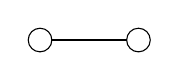
\begin{tikzpicture}
\draw (0,0) -- (1.25,0);
\draw[fill=white] (0,0) circle[radius=0.15];
\draw[fill=white] (1.25,0) circle[radius=0.15];
\end{tikzpicture}
\end{center}
We immediately see that we have two fundamental roots, i.e.\ $\Pi = \{\pi_1,\pi_2\}$, since there are two circles in the diagram. The bond number is $n_{12} = 1$, so the two fundamental roots have the same length. Moreover, by definition
\bse
1=n_{12} = C_{12}C_{21}
\ese
and since the off-diagonal entries of the Cartan matrix are non-positive integers, the only possibility is $C_{12}=C_{21}=-1$, so that we have
\bse
C = \biggl( \begin{matrix}2 & -1\\ -1 & 2\end{matrix}\biggr).
\ese
To determine the angle $\varphi$ between $\pi_1$ and $\pi_2$, recall that
\bse
1 = n_{12} = 4 \cos^2\varphi,
\ese
and hence $|\cos\varphi|=\frac{1}{2}$. There are two solutions, namely $\varphi=60^\circ$ and $\varphi=120^\circ$.
\begin{center}
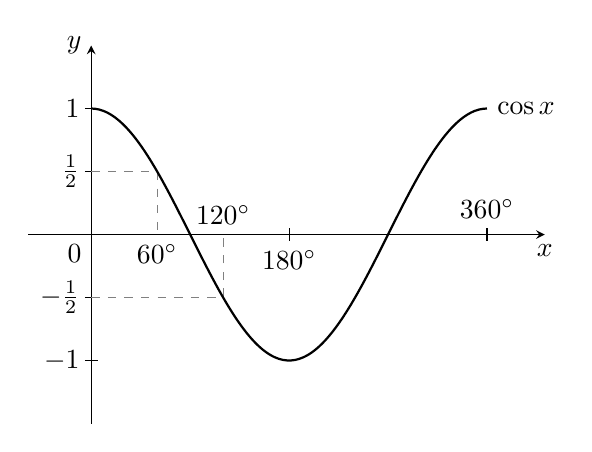
\begin{tikzpicture}[xscale=0.8,yscale=1.6]
\draw[->] (-1,0) -- (7.2,0) node[below] {$x$};
\draw[->] (0,-1.5) -- (0,1.5) node[left] {$y$};
\foreach \i/\j in {-2/-1,-1/-\frac{1}{2},1/\frac{1}{2},2/1} {
\draw (-0.1,0.5*\i) -- (0.1,0.5*\i) node[left=3pt] {$\j$};
}
\draw (0,0) node[below left] {$0$};
\draw[gray,dashed] (0,0.5) -| (pi/3,0);
\draw (pi/3,0) node[below] {$60^\circ$};
\draw[gray,dashed] (0,-0.5) -| (2*pi/3,0);
\draw (2*pi/3,0) node[above] {$120^\circ$};
\draw (pi,0.05) -- (pi,-0.05) node[below] {$180^\circ$};
\draw (2*pi,-0.05) -- (2*pi,0.05) node[above] {$360^\circ$};
\draw[thick,smooth,samples=100,variable=\x,domain=0:2*pi] plot(\x,{cos(deg(\x))}) node[right] {$\cos x$};
\end{tikzpicture}
\end{center}
By definition, we have
\bse
\cos \varphi = \frac{\kappa^*(\pi_1,\pi_2)}{|\pi_1|\,|\pi_2|},
\ese
and therefore
\bse
0 > C_{12} = 2\frac{\kappa^*(\pi_1,\pi_2)}{\kappa^*(\pi_1,\pi_1)} = 2\frac{|\pi_1|\,|\pi_2|\cos\varphi}{\kappa^*(\pi_1,\pi_1)} = 2\frac{|\pi_2|}{|\pi_1|}\cos\varphi.
\ese
It follows that $\cos\varphi<0$, and hence $\varphi = 120^\circ$. We can thus plot the two fundamental roots in a plane as follows.
\begin{center}
\begin{tikzpicture}[scale=2]
\draw[thin,lightgray] (-1.5,0) -- (1.5,0);
\draw[thin,lightgray] (0,-1.25) -- (0,1.25);
\draw[thick,->] (0,0) -- (1,0) node[above right] {$\pi_1$};
\draw[thick,->] (0,0) -- (cos 120,sin 120) node[above left] {$\pi_2$};
\end{tikzpicture}
\end{center}
We can determine all the other roots in $\Phi$ by repeated action of the Weyl group. For instance, we easily find that $s_{\pi_1}(\pi_1) = -\pi_1$ and $s_{\pi_2}(\pi_2) = -\pi_2$. We also have
\bse
s_{\pi_1}(\pi_2)  =  \pi_2-2\frac{\kappa^*(\pi_1,\pi_2)}{\kappa^*(\pi_1,\pi_1)}\pi_1 = \pi_2 -2 (-\tfrac{1}{2}) \pi_1 = \pi_1+\pi_2.
\ese
Finally, we have $s_{\pi_1+\pi_2}(\pi_1+\pi_2)=-(\pi_1+\pi_2)$.  Any further action by Weyl transformations simply permutes these roots. Hence, we have
\bse
\Phi=\{\pi_1,-\pi_1,\pi_2,-\pi_2,\pi_1+\pi_2,-(\pi_1+\pi_2)\}
\ese
and these are all the roots.
\begin{center}
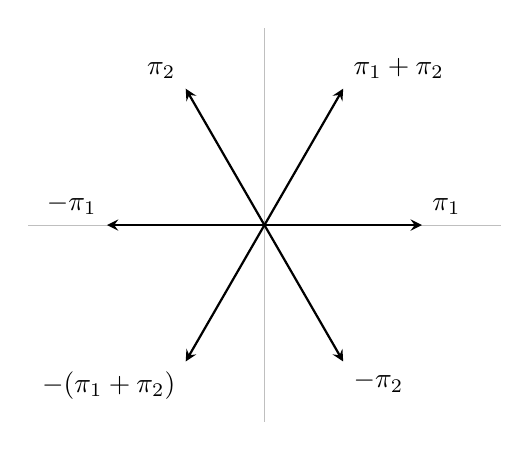
\begin{tikzpicture}[scale=2]
\draw[thin,lightgray] (-1.5,0) -- (1.5,0);
\draw[thin,lightgray] (0,-1.25) -- (0,1.25);
\draw[thick,->] (0,0) -- (1,0) node[above right] {$\pi_1$};
\draw[thick,->] (0,0) -- (cos 120,sin 120) node[above left] {$\pi_2$};
\draw[thick,->] (0,0) -- (-1,0) node[above left] {$-\pi_1$};
\draw[thick,->] (0,0) -- (-cos 120,-sin 120) node[below right] {$-\pi_2$};
\draw[thick,->] (0,0) -- (cos 60,sin 60) node[above right] {$\pi_1+\pi_2$};
\draw[thick,->] (0,0) -- (-cos 60,-sin 60) node[below left] {$-(\pi_1+\pi_2)$};
\end{tikzpicture}
\end{center}
Since $H^*=\lspan_\C(\Pi)$, we have $\dim H^*=2$, thus the dimension of the Cartan  subalgebra is also $2$. Since $|\Phi|=6$, we know that any Cartan-Weyl basis of the Lie algebra $A_2$ must have $2+6=8$ elements. Hence, the dimension of $A_2$ is 8. 

To complete our reconstruction of $A_2$, we would now like to understand how its bracket behaves. This amounts to finding its structure constants. Note that since $\dim A_2 = 8$, the structure constants $C^k_{\phantom{h}ij}$ consist of $8^3=512$ complex numbers (not all unrelated, of course).

Denote by $\{h_1,h_2,e_3,\ldots,e_8\}$ a Cartan-Weyl basis of $A_2$, so that $H=\lspan_\C(\{h_1,h_2\})$ and the $e_\alpha$ are eigenvectors of every $h\in H$.
Since $A_2$ is simple, $H$ is abelian and hence
\bse
[h_1,h_2] = 0 \quad \Rightarrow \quad C^k_{\phantom{k}12}=C^k_{\phantom{k}21} = 0, \quad \forall \, 1\leq k \leq 8.
\ese
To each $e_\alpha$, for $3\leq \alpha \leq 8$, there is an associated $\lambda_\alpha\in\Phi$ such that
\bse
\forall \, h \in H : \ \ad(h)e_\alpha = \lambda_\alpha(h) e_\alpha.
\ese
In particular, for the basis elements $h_1,h_2$,
\bi{rCl}
[h_1,e_\alpha] & = & \ad(h_1)e_\alpha = \lambda_\alpha(h_1) e_\alpha,\\
{[h_2,e_\alpha]} & = & \ad(h_2)e_\alpha = \lambda_\alpha(h_2) e_\alpha,
\ei
so that we have
\bi{rCl}
C^1_{\phantom{1}1\alpha}=C^2_{\phantom{2}1\alpha}=0, &\quad & C^\alpha_{\phantom{\alpha}1\alpha} = \lambda_\alpha(h_1) , \quad \forall \, 3\leq \alpha \leq 8,\\
C^1_{\phantom{1}2\alpha}=C^2_{\phantom{2}2\alpha}=0, &\quad & C^\alpha_{\phantom{\alpha}2\alpha} = \lambda_\alpha(h_2) , \quad \forall \, 3\leq \alpha \leq 8.
\ei
Finally, we need to determine $[e_\alpha,e_\beta]$. By using the Jacobi identity, we have
\bi{rCl}
[h_i,[e_\alpha,e_\beta]] & = & - [e_\alpha,[e_\beta,h_i]] -[e_\beta,[h_i,e_\alpha]] \\
& = & - [e_\alpha,-\lambda_\beta(h_i)e_\beta] -[e_\beta,\lambda_\alpha(h_i)e_\alpha] \\
& = & \lambda_\beta(h_i) [e_\alpha,e_\beta] +\lambda_\alpha(h_i)[e_\alpha,e_\beta]\\
& = & (\lambda_\alpha(h_i)+\lambda_\beta(h_i) )[e_\alpha,e_\beta]  ,
\ei
that is,
\bse
\ad(h_i)[e_\alpha,e_\beta] =  (\lambda_\alpha(h_i)+\lambda_\beta(h_i) )[e_\alpha,e_\beta].
\ese

If $\lambda_\alpha+\lambda_\beta\in\Phi$, we have $[e_\alpha,e_\beta]=\xi e_\gamma$ for some $3\leq \gamma \leq 8$ and $\xi \in \C$. Let us label the roots in our previous plot as
\begin{center}
\def\arraystretch{1.25}
\setlength\tabcolsep{10pt}
\begin{tabular}{c|c|c|c|c|c}
$\lambda_3$ & $\lambda_4$ & $\lambda_5$ & $\lambda_6$ & $\lambda_7$ & $\lambda_8$\\
\hline
$\pi_1$ & $\pi_2$ & $\pi_1+\pi_2$ & $-\pi_1$ & $-\pi_2$ & $-(\pi_1+\pi_2)$ 
\end{tabular}
\end{center}
Then, for example
\bse
\ad(h)[e_3,e_4] = (\pi_1+\pi_2)(h) [e_3,e_4],
\ese
and hence $[e_3,e_4]$ is an eigenvector of $\ad(h)$ with eigenvalues $(\pi_1+\pi_2)(h)$. But so is $e_5$! Hence, we must have $[e_3,e_4]=\xi e_5$ for some $\xi \in \C$. Similarly, $[e_5,e_7]=\xi e_3$, and so on.

If $\lambda_\alpha+\lambda_\beta\notin\Phi$, then in order for the equation above to hold, we must have either $[e_\alpha,e_\beta]=0$ (so both sides are zero), or $\lambda_\alpha(h)+\lambda_\beta(h)=0$ for all $h$, i.e.\ $\lambda_\alpha+\lambda_\beta=0$ as a functional. In the latter case, we must have $[e_\alpha,e_\beta]\in H$. This follows from a stronger version of the maximality property of the Cartan subalgebra $H$ of a simple Lie algebra $L$, namely that
\bse
\big(\forall \, h \in H : [h,x] = 0 \big)  \Rightarrow x\in H.
\ese
Summarising, we have
\bse
[e_\alpha,e_\beta] =
\begin{cases}
\xi e_\gamma & \text{if } \lambda_\alpha+\lambda_\beta\in\Phi\\
\in H & \text{if } \lambda_\alpha+\lambda_\beta=0\\
0 & \text{otherwise }
\end{cases}
\ese
and these relations con be used to determine the remaining structure constants of $A_2$.


























% \newpage

% \section{Representation theory of Lie groups and Lie algebras}
% 
Lie groups and Lie algebras are used in physics mostly in terms of what are called representations. Very often they are even defined in terms of their concrete representations. We took a more abstract approach by defining a Lie group as a smooth manifold with a compatible group structure, and its associated Lie algebra as the space of left-invariant vector fields, which we then showed to be isomorphic to the tangent space at the identity.

\subsection{Representations of Lie algebras}

\bd
Let $L$ be a Lie algebra. A \emph{representation}\index{representation} of $L$ is a Lie algebra homomorphism
\bse
\rho\cl L \xrightarrow{\sim} \End(V),
\ese
where $V$ is some finite-dimensional vector space over the same field as $L$.
\ed
Recall that a linear map $\rho\cl L \xrightarrow{\sim} \End(V)$ is a Lie algebra homomorphism if
\bse
\forall \, x,y\in L : \ \rho([x,y]) = [\rho(x),\rho(y)]:=\rho(x)\circ\rho(y)-\rho(y)\circ\rho(x),
\ese
where the right hand side is the natural Lie bracket on $\End(V)$.

\bd
Let $\rho\cl L \xrightarrow{\sim}\End(V)$ be a representation of $L$.
\ben[label=\roman*)]
\item The vector space $V$ is called the \emph{representation space} of $\rho$.
\item The \emph{dimension}\index{dimension!representation} of the representation $\rho$ is $\dim V$.
\een
\ed

\be
Consider the Lie algebra $\sl(2,\C)$. We constructed a basis $\{X_1,X_2,X_3\}$ satisfying the relations
\bi{rCl}
[X_1,X_2] & = & 2X_2,\\
{[X_1,X_3]} & = & -2X_3,\\
{[X_2,X_3]} & = & X_1.
\ei
Let $\rho\cl\sl(2,\C)\xrightarrow{\sim}\End(\C^2)$ be the linear map defined by
\bse
\rho(X_1) := \biggl(\begin{matrix}1& 0\\ 0 & -1\end{matrix}\biggr), \qquad \rho(X_2) := \biggl(\begin{matrix}0& 1\\ 0 & 0\end{matrix}\biggr), \qquad \rho(X_3) := \biggl(\begin{matrix}0& 0\\ 1 & 0\end{matrix}\biggr)
\ese
(recall that a linear map is completely determined by its action on a basis, by linear continuation). To check that $\rho$ is a representation of $\sl(2,\C)$, we calculate
\bi{rCl}
[\rho(X_1),\rho(X_2)] & = & \biggl(\begin{matrix}1& 0\\ 0 & -1\end{matrix}\biggr)\biggl(\begin{matrix}0& 1\\ 0 & 0\end{matrix}\biggr)-\biggl(\begin{matrix}0& 1\\ 0 & 0\end{matrix}\biggr)\biggl(\begin{matrix}1& 0\\ 0 & -1\end{matrix}\biggr)\\
%& = & \biggl(\begin{matrix}0& 1\\ 0 & 0\end{matrix}\biggr)-\biggl(\begin{matrix}0& -1\\ 0 & 0\end{matrix}\biggr)\\
& = & \biggl(\begin{matrix}0& 2\\ 0 & 0\end{matrix}\biggr)\\
& = &\rho(2X_2)\\
& = &\rho([X_1,X_2]).
\ei
Similarly, we find
\bi{rCl}
[\rho(X_1),\rho(X_3)] & = & \rho([X_1,X_3]),\\
{[\rho(X_2),\rho(X_3)]} & = & \rho([X_2,X_3]).
\ei
By linear continuation, $\rho([x,y]) = [\rho(x),\rho(y)]$ for any $x,y\in \sl(2,\C)$ and hence, $\rho$ is a $2$-dimensional representation of $\sl(2,\C)$ with representation space $\C^2$. Note that we have
\bi{rCl}
\im_\rho(\sl(2,\C)) & = & \biggl\{ \biggl(\begin{matrix}a& b\\ c & d\end{matrix}\biggr) \in \End(\C^2) \ \Big| \ a+d = 0 \biggr\}\\[3pt]
& = & \{\phi\in\End(\C^2)\mid \tr \phi = 0\}.
\ei
This is how $\sl(2,\C)$ is often defined in physics courses, i.e.\ as the algebra of $2\times 2$ complex traceless matrices.
\ee

Two representations of a Lie algebra can be related in the following sense.

\bd
Let $L$ be a Lie algebra and let 
\bse
\rho_1\cl L \xrightarrow{\sim} \End(V_1), \qquad 
\rho_2\cl L \xrightarrow{\sim} \End(V_2)
\ese
be representations of $L$. A linear map $f\cl V_1\xrightarrow{\sim}V_2$ is a \emph{homomorphism of representations} if
\bse
\forall \, x \in L : \ f\circ \rho_1(x) = \rho_2(x)\circ f.
\ese
Equivalently, if the following diagram commutes for all $x\in L$.
\bse
\begin{tikzcd}
V_1 \ar[rr,"f"] \ar[dd,"\rho_1(x)"']&& V_2\ar[dd,"\rho_2(x)"]\\
&&\\
V_1\ar[rr,"f"] && V_2
\end{tikzcd}
\ese
\ed
If in addition $f\cl V_1\xrightarrow{\sim}V_2$ is a linear isomorphism, then $f^{-1}\cl V_2\xrightarrow{\sim}V_1$ is automatically a homomorphism of representations, since
\bi{rCl}
f\circ \rho_1(x) = \rho_2(x)\circ f &\ \Leftrightarrow\ & f^{-1}\circ (f\circ \rho_1(x)) \circ f^{-1} = f^{-1}\circ(\rho_2(x)\circ f)\circ f^{-1} \\
& \Leftrightarrow & \rho_1(x) \circ f^{-1} = f^{-1}\circ\rho_2(x).
\ei
\bd
An \emph{isomorphism of representations}\index{isomorphism!of representations} of Lie algebras is a bijective homomorphism of representations.
\ed
Isomorphic representations necessarily have the same dimension.
\be
Consider $\so(3,\R)$, the Lie algebra of the rotation group $\SO(3,\R)$. It is a $3$-dimensional Lie algebra over $\R$. It has a basis $\{J_1,J_2,J_3\}$ satisfying
\bse
[J_i,J_j] = C^{k}_{\phantom{k}ij} J_k,
\ese
where the structure constants $C^{k}_{\phantom{k}ij}$ are defined by first ``pulling the index $k$ down'' using the Killing form $\kappa_{ab}=C^{m}_{\phantom{m}an} C^{n}_{\phantom{n}bm}$ to obtain $C_{kij}:=\kappa_{km} C^{m}_{\phantom{m}ij}$, and then setting
\bse
C_{kij}:= \varepsilon_{ijk} := \begin{cases}\ 1 & \text{ if $(i\, j\, k)$ is an even permutation of $(1\, 2\, 3)$} \\
-1 & \text{ if $(i\, j\, k)$ is an odd permutation of $(1\, 2\, 3)$}\\
\ 0 & \text{ otherwise}.\end{cases}
\ese
By evaluating these, we find
\bi{rCl}
[J_1,J_2] & = & J_3,\\
{[J_2,J_3]} & = & J_1,\\
{[J_3,J_1]} & = & J_2.
\ei
Define a linear map $\rho_{\mathrm{vec}}\cl\so(3,\R)\xrightarrow{\sim}\End(\R^3)$ by
\bse
\rho_{\mathrm{vec}}(J_1) := \begin{pmatrix}0 & 0 & 0\\ 0 & 0 & -1\\ 0 & 1 & 0\end{pmatrix}, \qquad \rho_{\mathrm{vec}}(J_2) := \begin{pmatrix}0 & 0 & 1\\ 0 & 0 & 0\\ -1 & 0 & 0\end{pmatrix}, \qquad \rho_{\mathrm{vec}}(J_3) :=\begin{pmatrix}0 & -1 & 0\\ 1 & 0 & 0\\ 0 & 0 & 0\end{pmatrix}.
\ese
You can easily check that this is a representation of $\so(3,\R)$. However, as you may be aware from quantum mechanics, there is another representation of $\so(3,\R)$, namely
\bse
\rho_{\mathrm{spin}}\cl\so(3,\R)\xrightarrow{\sim}\End(\C^2),
\ese
with $\C^2$ understood as a $4$-dimensional $\R$-vector space, defined by
\bse
\rho_{\mathrm{spin}}(J_1) := -\frac{\mathrm{i}}{2}\, \sigma_1, \qquad \rho_{\mathrm{spin}}(J_2) := -\frac{\mathrm{i}}{2}\, \sigma_2, \qquad \rho_{\mathrm{spin}}(J_3) := -\frac{\mathrm{i}}{2}\, \sigma_3,
\ese
where $\sigma_1,\sigma_2,\sigma_3$ are the Pauli matrices
\bse
\sigma_1 = \biggl(\begin{matrix}0& 1\\ 1 & 0\end{matrix}\biggr), \qquad \sigma_2 = \biggl(\begin{matrix}0& -\mathrm{i}\\ \mathrm{i} & 0\end{matrix}\biggr), \qquad
\sigma_3 = \biggl(\begin{matrix}1& 0\\ 0 & -1\end{matrix}\biggr).
\ese
You can again check that this is a representation of $\so(3,\R)$. Since
\bse
\dim \R^3 = 3 \neq 4 = \dim \C^2,
\ese
the representations $\rho_{\mathrm{vec}}$ and $\rho_{\mathrm{spin}}$ are not isomorphic. 
\ee
Any (non-abelian) Lie algebra always has at least two special representations.

\bd
Let $L$ be a Lie algebra.  A \emph{trivial representation} of $L$ is defined by
\bi{rrCl}
\rho_{\mathrm{trv}} \cl & L & \xrightarrow{\sim} & \End(V)\\
& x & \mapsto & \rho_{\mathrm{trv}}(x) := 0,
\ei
where $0$ denotes the trivial endomorphism on $V$.
\ed
\bd
The \emph{adjoint representation}\index{adjoint representation} of $L$ is
\bi{rrCl}
\rho_{\mathrm{adj}} \cl & L & \xrightarrow{\sim} & \End(L)\\
& x & \mapsto & \rho_{\mathrm{adj}}(x) := \ad(x).
\ei
\ed

These are indeed representations since we have already shown that $\ad$ is a Lie algebra homomorphism, while for the trivial representations we have
\bse
\forall\, x,y \in L : \ \rho_\mathrm{trv}([x,y]) = 0 = [\rho_\mathrm{trv}(x),\rho_\mathrm{trv}(y)].
\ese

\bd
A representation $\rho\cl L \xrightarrow{\sim} \End(V)$ is called \emph{faithful} if $\rho$ is injective, i.e.\
\bse
\dim(\im_\rho(L)) = \dim L.
\ese
\ed

\be
All representations considered so far are faithful, except for the trivial representations whenever the Lie algebra $L$ is not itself trivial. Consider, for instance, the adjoint representation. We have
\bi{rCl}
\ad(x) = \ad(y) & \Leftrightarrow & \forall \, z \in L :  \ad(x)z = \ad(y)z\\
 & \Leftrightarrow & \forall \, z \in L :  [x,z] = [y,z]\\
 & \Leftrightarrow & \forall \, z \in L :  [x-y,z] = 0.
\ei
If $L$ is trivial, then any representation is faithful. Otherwise, there is some non-zero $z\in L$, hence we must have $x-y=0$, so $x=y$, and thus $\ad$ is injective.
\ee

\bd
Given two representations $\rho_1\cl L \xrightarrow{\sim} \End(V_1)$,  $\rho_2\cl L \xrightarrow{\sim} \End(V_2)$, we can construct nue representations called
\ben[label=\roman*)]
\item the \emph{direct sum representation}
\bi{rrCl}
\rho_1\oplus \rho_2 \cl & L &\xrightarrow{\sim} &\End(V_1\oplus V_2)\\
& x & \mapsto & (\rho_1\oplus \rho_2) (x)  := \rho_1(x)\oplus \rho_2(x)
\ei
\item the \emph{tensor product representation}
\bi{rrCl}
\rho_1\otimes \rho_2 \cl & L &\xrightarrow{\sim} &\End(V_1\times V_2)\\
& x & \mapsto & (\rho_1\otimes \rho_2) (x)  := \rho_1(x)\otimes \id_{V_2}+\id_{V_1}\otimes \rho_2(x).
\ei
\een
\ed

\be
The direct sum representation $\rho_{\mathrm{vec}}\oplus \rho_{\mathrm{spin}}\cl \so(3,\R)\xrightarrow{\sim}\End(\R^3\oplus\C^2)$ given in block-matrix form by
\bse
(\rho_{\mathrm{vec}}\oplus \rho_{\mathrm{spin}})(x) = \left(\begin{array}{c|c} \rho_{\mathrm{vec}}(x) & 0 \\ \hline 0 & \rho_{\mathrm{spin}}(x)\end{array}\right)
\ese
is a $7$-dimensional representation of $\so(3,\R)$.
\ee

\bd
A representation $\rho\cl L \xrightarrow{\sim} \End(V)$ is called \emph{reducible} if there exists a non-trivial vector subspace $U\se V$ which is invariant under the action of $\rho$, i.e.\
\bse
\forall \, x\in L: \forall \, u\in U : \ \rho(x)u\in U.
\ese
In other words, $\rho$ restricts to a representation $\rho|_U\cl L \xrightarrow{\sim} \End(U)$. 
\ed
\bd
A representation is \emph{irreducible} if it is not reducible.
\ed
\be
\ben[label=\roman*)]
\item The representation $\rho_{\mathrm{vec}}\oplus \rho_{\mathrm{spin}}\cl \so(3,\R)\xrightarrow{\sim}\End(\R^3\oplus\C^2)$ is reducible since, for example, we have a subspace $\R^3\oplus 0$ such that
\bse
\forall \, x \in \so(3,\R): \forall \, u\in \R^3\oplus 0 : \ (\rho_{\mathrm{vec}}\oplus \rho_{\mathrm{spin}}) (x)u\in\R^3\oplus 0.
\ese
\item The representations $\rho_{\mathrm{vec}}$ and $\rho_{\mathrm{spin}}$ are both irreducible.
\een
\ee

\br
Just like the simple Lie algebras are the building blocks of all semi-simple Lie algebras, the irreducible representations of a semi-simple Lie algebra are the building blocks of all finite-dimensional representations of the Lie algebra. Any such representation con be decomposed as the direct sum of irreducible representations, which can then be classified according to their so-called \emph{highest weights}.
\er

\subsection{The Casimir operator}

To every representation $\rho$ of a compact Lie algebra (i.e.\ the Lie algebra of a compact Lie group) there is associated an operator $\Omega_\rho$, called the Casimir operator. We will need some preparation in order to define it.

\bd
Let $\rho\cl L \xrightarrow{\sim} \End(V)$ be a representation of a complex Lie algebra $L$. We define the \emph{$\rho$-Killing form}\index{Killing form} on $L$ as 
\bi{rrCl}
\kappa_\rho \cl & L \times L & \xrightarrow{\sim} & \C\\
& (x,y) & \mapsto & \kappa_\rho(x,y) := \tr(\rho(x)\circ\rho(y)).
\ei
\ed
Of course, the Killing form we have considered so far is just $\kappa_{\ad}$. Similarly to $\kappa_{\ad}$, every $\kappa_\rho$ is symmetric and associative with respect to the Lie bracket of $L$. 
\bp
Let $\rho\cl L \xrightarrow{\sim} \End(V)$ be a faithful representation of a complex semi-simple Lie algebra $L$. Then, $\kappa_\rho$ is non-degenerate.
\ep
Hence, $\kappa_\rho$ induces an isomorphism $L\xrightarrow{\sim}L^*$ via
\bse
L \ni x \mapsto \kappa_\rho(x,-) \in L^*.
\ese
Recall that if $\{X_1,\ldots,X_{\dim L}\}$ is a basis of $L$, then the dual basis $\{\widetilde X^1,\ldots,\widetilde X^{\dim L}\}$ of $L^*$ is defined by
\bse
\widetilde X^i(X_j) = \delta_j^i.
\ese
By using the isomorphism induced by $\kappa_\rho$, we can find some $\xi_1,\ldots,\xi_{\dim L}\in L$ such that we have $\kappa(\xi_i,-)=\widetilde X^i$ or, equivalently,
\bse
\forall \, x\in L : \ \kappa_{\rho}(x,\xi_i) = \widetilde X^i(x).
\ese
We thus have
\bse
\kappa_\rho(X_i,\xi_j) = \delta_{ij} := \begin{cases}1 & \text{if }i\neq j\\ 0 & \text{otherwise.}\end{cases}
\ese

\bp
Let $\{X_i\}$ and $\{\xi_j\}$ be defined as above. Then
\bse
[X_j,\xi_k] = \sum_{m = 1}^{\dim L} C^{k}_{\phantom{k}mj}\xi_m, 
\ese
where $C^{k}_{\phantom{k}mj}$ are the structure constants with respect to $\{X_i\}$.
\ep

\bq
By using the associativity of $\kappa_\rho$, we have
\bse
\kappa_\rho(X_i,[X_j,\xi_k]) = \kappa_\rho([X_i,X_j],\xi_k) = C^{m}_{\phantom{m}ij} \kappa_\rho(X_m,\xi_k) = C^{m}_{\phantom{m}ij} \delta_{mk} = C^{k}_{\phantom{k}ij}.
\ese
But we also have
\bse
\kappa_\rho\Bigl(X_i,\sum_{m=1}^{\dim L}C^{k}_{\phantom{k}mj} \xi_m \Bigr) = \sum_{m=1}^{\dim L}C^{k}_{\phantom{k}mj} \kappa_\rho(X_i,\xi_m)  = \sum_{m=1}^{\dim L}C^{k}_{\phantom{k}mj} \delta_{im} = C^{k}_{\phantom{k}ij}.
\ese
Therefore
\bse
\forall \, 1\leq i \leq \dim L : \ \kappa_\rho\Bigl(X_i,[X_j,\xi_k]-\sum_{m=1}^{\dim L}C^{k}_{\phantom{k}mj} \xi_m \Bigr) = 0
\ese
and hence, the result follows from the non-degeneracy of $\kappa_{\rho}$.
\eq
We are now ready to define the Casimir operator and prove the subsequent theorem.
\bd
Let $\rho\cl L \xrightarrow{\sim} \End(V)$ be a faithful representation of a complex (compact) Lie algebra $L$  and let $\{X_1,\ldots,X_{\dim L}\}$ be a basis of $L$. The \emph{Casimir operator}\index{Casimir operator} associated to the representation $\rho$ is the endomorphism $\Omega_\rho\cl V \xrightarrow{\sim} V$
\bse
\Omega_\rho := \sum_{i=1}^{\dim L} \rho(X_i) \circ \rho(\xi_i).
\ese
\ed

\begin{theorem}
Let $\Omega_\rho$ the Casimir operator of a representation $\rho\cl L \xrightarrow{\sim} \End(V)$. Then
\bse
\forall \, x \in L : \ [\Omega_\rho,\rho(x)] = 0,
\ese
that is, $\Omega_\rho$ commutes with every endomorphism in $\im_\rho(L)$.
\end{theorem}

\bq
Note that the bracket above is that on $\End(V)$. Let $x=x^kX_k\in L$. Then
\bi{rCl}
[\Omega_\rho,\rho(x)] & = &  \biggl[\, \sum_{i=1}^{\dim L} \rho(X_i) \circ \rho(\xi_i), \rho(x^kX_k)\biggr]\\
& = & \sum_{i,k=1}^{\dim L} x^k [\rho(X_i) \circ \rho(\xi_i), \rho(X_k)].
\ei
Observe that if the Lie bracket as the commutator with respect to an associative product, as is the case for $\End(V)$, we have
\bi{rCl}
[AB,C] & = & ABC - CBA \\
& = & ABC - CBA -ACB +ACB \\
& = & A[B,C] + [A,C]B. 
\ei
Hence, by applying this, we obtain
\bi{rCl}
\sum_{i,k=1}^{\dim L} x^k [\rho(X_i) \circ \rho(\xi_i), \rho(X_k)] & = & \sum_{i,k=1}^{\dim L} x^k \bigl(\rho(X_i) \circ [\rho(\xi_i), \rho(X_k)]+[\rho(X_i) , \rho(X_k)]\circ \rho(\xi_i)\bigr)\\
 & = & \sum_{i,k=1}^{\dim L} x^k \bigl(\rho(X_i) \circ \rho([\xi_i, X_k])+\rho([X_i,X_k])\circ \rho(\xi_i)\bigr)\\
 & = & \sum_{i,k,m=1}^{\dim L} x^k \bigl(\rho(X_i) \circ \rho(-C^{i}_{\phantom{i}mk}\xi_m)+\rho(C^{m}_{\phantom{m}ik}X_m)\circ \rho(\xi_i)\bigr)\\
 & = & \sum_{i,k,m=1}^{\dim L} x^k \bigl(-C^{i}_{\phantom{i}mk}\rho(X_i) \circ \rho(\xi_m)+C^{m}_{\phantom{m}ik}\rho(X_m)\circ \rho(\xi_i)\bigr)\\
 & = & \sum_{i,k,m=1}^{\dim L} x^k \bigl(-C^{i}_{\phantom{i}mk}\rho(X_i) \circ \rho(\xi_m)+C^{i}_{\phantom{i}mk}\rho(X_i)\circ \rho(\xi_m)\bigr)\\
& = & 0,
\ei
after swapping the dummy summation indices $m$ and $i$ in the second term.
\eq

\begin{lemma}[Schur]
If $\rho\cl L \xrightarrow{\sim} \End(V)$ is irreducible, then any operator $S$ which commutes with every endomorphism in $\im_\rho(L)$ has the form
\bse
S = c_\rho \id_V
\ese
for some constant $c_\rho\in \C$ (or $\R$, if $L$ is a real Lie algebra).
\end{lemma}
It follows immediately that $\Omega_\rho = c_\rho \id_V$ for some $c_\rho$ but, in fact, we can say more.
\bp
The Casimir operator of $\rho\cl L \xrightarrow{\sim} \End(V)$ is $\Omega_\rho = c_\rho \id_V$, where
\bse
c_\rho = \frac{\dim L}{\dim V}.
\ese
\ep
\bq
We have
\bse
\tr(\Omega_\rho) = \tr(c_\rho\id_V) = c_\rho \dim V
\ese
and
\bi{rCl}
\tr(\Omega_\rho) & = & \tr \biggl(\, \sum_{i=1}^{\dim L} \rho(X_i) \circ \rho(\xi_i) \biggr)\\
 & = &  \sum_{i=1}^{\dim L} \tr(\rho(X_i) \circ \rho(\xi_i) )\\
 & = &  \sum_{i=1}^{\dim L} \kappa_\rho(X_i,\xi_i)\\
 & = &  \sum_{i=1}^{\dim L} \delta_{ii}\\
 & = &  \dim L ,
\ei
which is what we wanted.
\eq

\be
Consider the Lie algebra $\so(3,\R)$ with basis $\{J_1,J_2,J_3\}$ satisfying
\bse
[J_i,J_j] = \varepsilon_{ijk}J_k,
\ese
where we assume the summation convention on the lower index $k$. Recall that the representation $\rho_{\mathrm{vec}}\cl\so(3,\R)\xrightarrow{\sim}\End(\R^3)$ is defined by
\bse
\rho_{\mathrm{vec}}(J_1) := \begin{pmatrix}0 & 0 & 0\\ 0 & 0 & -1\\ 0 & 1 & 0\end{pmatrix}, \qquad \rho_{\mathrm{vec}}(J_2) := \begin{pmatrix}0 & 0 & 1\\ 0 & 0 & 0\\ -1 & 0 & 0\end{pmatrix}, \qquad \rho_{\mathrm{vec}}(J_3) :=\begin{pmatrix}0 & -1 & 0\\ 1 & 0 & 0\\ 0 & 0 & 0\end{pmatrix}.
\ese
Let us first evaluate the components of $\kappa_{\rho_{\mathrm{vec}}}$. We have
\bi{rCl}
(\kappa_{\rho_{\mathrm{vec}}})_{11} := \kappa_{\rho_{\mathrm{vec}}}(J_1,J_1) & = & \tr(\rho_{\mathrm{vec}}(J_1)\circ \rho_{\mathrm{vec}}(J_1)) \\
& = & \tr((\rho_{\mathrm{vec}}(J_1))^2)\\
& = & \tr\begin{pmatrix}0 & 0 & 0\\ 0 & 0 & -1\\ 0 & 1 & 0\end{pmatrix}^{\negmedspace 2}\\
& = & \tr\begin{pmatrix}0 & 0 & 0\\ 0 & -1 & 0\\ 0 & 0 & -1\end{pmatrix}\\
& = & -2.
\ei
After calculating the other components similarly, we find
\bse
[(\kappa_{\rho_{\mathrm{vec}}})_{ij}] = \begin{pmatrix}-2 & 0 & 0\\ 0 & -2 & 0\\ 0 & 0 & -2\end{pmatrix}.
\ese
Thus, $\kappa_{\rho_{\mathrm{vec}}}(J_i,\xi_j)=\delta_{ij}$ requires that we define $\xi_i := -\tfrac{1}{2} J_i$. Then, we have
\bi{rCl}
\Omega_{\rho_{\mathrm{vec}}} & := & \sum_{i=1}^{3} \rho_{\mathrm{vec}}(J_i) \circ \rho_{\mathrm{vec}}(\xi_i)\\
& = & \sum_{i=1}^{3} \rho_{\mathrm{vec}}(J_i) \circ \rho_{\mathrm{vec}}(-\tfrac{1}{2} J_i)\\
& = & -\frac{1}{2} \sum_{i=1}^{3} (\rho_{\mathrm{vec}}(J_i))^2\\
& = & -\frac{1}{2} \left( \begin{pmatrix}0 & 0 & 0\\ 0 & 0 & -1\\ 0 & 1 & 0\end{pmatrix}^{\negmedspace 2}+ \begin{pmatrix}0 & 0 & 1\\ 0 & 0 & 0\\ -1 & 0 & 0\end{pmatrix}^{\negmedspace 2} +\begin{pmatrix}0 & -1 & 0\\ 1 & 0 & 0\\ 0 & 0 & 0\end{pmatrix}^{\negmedspace 2}\ \right)\\
& = & -\frac{1}{2} \left( \begin{pmatrix}0 & 0 & 0\\ 0 & -1 & 0\\ 0 & 0 & -1\end{pmatrix}+ \begin{pmatrix}-1 & 0 & 0\\ 0 & 0 & 0\\ 0 & 0 & -1\end{pmatrix} +\begin{pmatrix}-1 & 0 & 0\\ 0 & -1 & 0\\ 0 & 0 & 0\end{pmatrix} \right)\\
& = & \begin{pmatrix}1 & 0 & 0\\ 0 & 1 & 0\\ 0 & 0 & 1\end{pmatrix}.
\ei
Hence $\Omega_{\rho_{\mathrm{vec}}}=c_{\rho_{\mathrm{vec}}}\id_{\R^3}$ with $c_{\rho_{\mathrm{vec}}} = 1$, which agrees with our previous theorem since
\bse
\frac{\dim \so(3,\R)}{\dim \R^3} = \frac{3}{3} = 1.
\ese
\ee

\be
Let us consider the Lie algebra $\so(3,\R)$ again, but this time with representation $\rho_{\mathrm{spin}}$. Recall that this is given by
\bse
\rho_{\mathrm{spin}}(J_1) := -\frac{\mathrm{i}}{2}\, \sigma_1, \qquad \rho_{\mathrm{spin}}(J_2) := -\frac{\mathrm{i}}{2}\, \sigma_2, \qquad \rho_{\mathrm{spin}}(J_3) := -\frac{\mathrm{i}}{2}\, \sigma_3,
\ese
where $\sigma_1,\sigma_2,\sigma_3$ are the Pauli matrices. Recalling that $\sigma_1^2=\sigma_2^2=\sigma_3^2=\id_{\C^2}$, we calculate
\bi{rCl}
(\kappa_{\rho_{\mathrm{spin}}})_{11} := \kappa_{\rho_{\mathrm{spin}}}(J_1,J_1) & = & \tr(\rho_{\mathrm{spin}}(J_1)\circ \rho_{\mathrm{spin}}(J_1)) \\
& = & \tr((\rho_{\mathrm{spin}}(J_1))^2)\\
& = &(-\tfrac{\mathrm{i}}{2})^2 \tr(\sigma_1^{2})\\
& = & -\tfrac{1}{4} \tr(\id_{\C^2})\\
& = & -1.
\ei
Note that $\tr(\id_{\C^2})=4$, since $\tr(\id_V)=\dim V$ and here $\C^2$ is considered as a $4$-dimensional vector space over $\R$. Proceeding similarly, we find that the components of $\kappa_{\rho_{\mathrm{spin}}}$ are
\bse
[(\kappa_{\rho_{\mathrm{spin}}})_{ij}] = \begin{pmatrix}-1 & 0 & 0\\ 0 & -1 & 0\\ 0 & 0 & -1\end{pmatrix}.
\ese
Hence, we define $\xi_i := - J_i$. Then, we have
\bi{rCl}
\Omega_{\rho_{\mathrm{spin}}} & := & \sum_{i=1}^{3} \rho_{\mathrm{spin}}(J_i) \circ \rho_{\mathrm{spin}}(\xi_i)\\
& = & \sum_{i=1}^{3} \rho_{\mathrm{spin}}(J_i) \circ \rho_{\mathrm{spin}}(-J_i)\\
& = & - \sum_{i=1}^{3} (\rho_{\mathrm{spin}}(J_i))^2\\
& = & - \Bigl(-\frac{\mathrm{i}}{2}\Bigr)^2\, \sum_{i=1}^{3} \sigma_i^2\\
& = & \frac{1}{4} \sum_{i=1}^{3} \id_{\C^2}\\
& = & \frac{3}{4}\id_{\C^2},
\ei
in accordance with the fact that
\bse
\frac{\dim \so(3,\R)}{\dim \C^2} = \frac{3}{4}.
\ese
\ee

\subsection{Representations of Lie groups}

We now turn to representations of Lie groups. Given a vector space $V$, recall that the subset of $\End(V)$ consisting of the invertible endomorphisms and denoted
\bse
\GL(V) \equiv \Aut(V):= \{\phi\in \End(V)\mid \det \phi \neq 0\},
\ese
forms a group under composition, called the automorphism group (or general linear group) of $V$. Moreover, if $V$ is a finite-dimensional $K$-vector space, then $V\cong_{\mathrm{vec}}K^{\dim V}$ and hence the group $\GL(V)$ can be given the structure of a Lie group via
\bse
\GL(V)\cong_{\mathrm{Lie \, grp}}\GL(K^{\dim V}):=\GL(\dim V,K).
\ese
This is, of course, if we have established a topology and a differentiable structure on $K^d$, as is the case for $\R^d$ and $\C^d$.
\bd
A \emph{representation}\index{representation} of a Lie group $(G,\bullet)$ is a Lie group homomorphism
\bse
R\cl G \to \GL(V)
\ese
for some finite-dimensional vector space $V$.
\ed
Recall that $R\cl G \to \GL(V)$ is a Lie group homomorphism if it is smooth and
\bse
\forall \, g_1,g_2\in G : R(g_1\bullet g_2) = R(g_1)\circ R( g_2).
\ese
Note that, as is the case with any group homomorphism, we have
\bse
R(e) = \id_V \qquad \text{and}\qquad R(g^{-1}) = R(g)^{-1}.
\ese
\be
Consider the Lie group $\SO(2,\R)$. As a smooth manifold, $\SO(2,\R)$ is isomorphic to the circle $S^1$. Let $U=S^1\sm\{p_0\}$, where $p$ is any point of $S^1$, so that we can define a chart $\theta\cl U \to [0,2\pi)\se\R$ on $S^1$ by mapping each point in $U$ to an ``angle'' in $[0,2\pi)$.
\bse
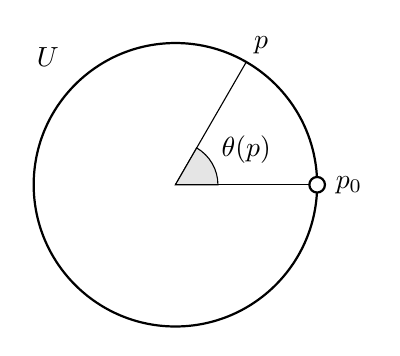
\begin{tikzpicture}[scale=0.9]
\draw[thick] (0,0) circle [radius=2];
\draw (0,0) -- (2,0);
\draw (0,0) -- (2*cos 60, 2* sin 60) node[above right=-1pt] {$p$};
\filldraw[fill=lightergray] (0,0) -- (0.6,0) arc (0:60:0.6) -- cycle;
\draw (1,0.5) node {$\theta(p)$};
\draw (-1.8,1.8) node {$U$};
\draw[thick,fill=white] (2,0) circle [radius=0.11] node[right=3pt] {$p_0$};
\end{tikzpicture}
\ese
The operation
\bse
p_1\bullet p_2:=(\theta(p_1)+\theta(p_2))\! \mod 2\pi
\ese
endows $S^1\cong_{\mathrm{diff}}\SO(2,\R)$ with the structure of a Lie group. Then, a representation of $\SO(2,\R)$ is given by
\bi{rrCl}
R\cl & \SO(2,\R) & \to & \GL(\R^2)\\
&  p & \mapsto & \biggl( \begin{matrix} \cos \theta(p) & \sin \theta(p) \\ -\sin \theta(p) & \cos \theta(p) \end{matrix}\biggr).
\ei
Indeed, the addition formul\ae for sine and cosine imply that
\bse
R(p_1\bullet p_2) = R(p_1)\circ R(p_2).   
\ese
\ee

\be
Let $G$ be a Lie group (we suppress the $\bullet$ in this example). For each $g\in G$, define the Adjoint map
\bi{rrCl}
\Ad_g \cl & G & \to & G\\
& h & \mapsto & g h g^{-1}.
\ei
Note the capital ``A'' to distinguish this from the adjoint map on Lie algebras. Since $\Ad_g$ is a composition of the Lie group multiplication and inverse map, it is a smooth map. Moreover, we have
\bse
\Ad_g(e) = geg^{-1} = gg^{-1} = e.
\ese
Hence, the push-forward of $\Ad_g$ at the identity is the map
\bse
({\Ad_g}_*)_e \cl  T_eG  \xrightarrow{\sim}   T_{\Ad_g(e)}G=T_eG.
\ese
Thus, we have $\Ad_g\in\End(T_eG)$. In fact, you can check that
\bse
({\Ad_{g^{-1}}}_*)_e\circ ({\Ad_g}_*)_e = ({\Ad_g}_*)_e\circ ({\Ad_{g^{-1}}}_*)_e = \id_{T_eG},
\ese
and hence we have, in particular, $\Ad_g\in\GL(T_eG)\cong_{\mathrm{Lie\,grp}}\GL(\mathcal{L}(G))$.

\noindent We can therefore construct a map
\bi{rrCl}
\Ad \cl & G & \to & \GL(T_eG)\\
& g & \mapsto & {\Ad_g}_*
\ei
which, as you can check, is a representation of $G$ on its Lie algebra.
\ee

\br
Since a representation $R$ of a Lie group $G$ is required to be smooth, we can always consider its differential or push-forward at the identity
\bse
(R_*)_e \cl T_eG \xrightarrow{\sim} T_{\id_V}\!\GL(V).
\ese
Since for any $A,B\in T_eG$ we have
\bse
(R_*)_e[A,B] =[(R_*)_eA,(R_*)_eB],
\ese
the map $(R_*)_e$ is a representation of the Lie algebra of $G$ on the vector space $\GL(V)$. In fact, in the previous example we have 
\bse
(\Ad_*)_e = \ad,
\ese
where $\ad$ is the adjoint representation of $T_eG$.
\er






















% \newpage

% \section{Reconstruction of a Lie group from its algebra}
% 

We have seen in detail how to construct a Lie algebra from a given Lie group. We would now like to consider the inverse question, i.e.\ whether, given a Lie algebra, we can construct a Lie group whose associated Lie algebra is the given one and, if this is the case, whether this correspondence is bijective.

% We will find that the answer to the first question is affirmative. Given a Lie algebra, we will construct a Lie group via something called the exponential map. However, we can already answer in the negative the second question. The Lie groups
% \bse
% \Ort(n,\R) := \{\phi\in \GL(n,\R)\}
% \ese
% and $\SU(2,\C)$ are an example of Lie groups which are not isomorphic but give rise to the same Lie algebra. Hence, the correspondence between Lie groups and Lie algebras cannot be bijective. 

\subsection{Integral curves}

\bd
Let $M$ be a smooth manifold and let $Y\in \Gamma(TM)$. An \emph{integral curve}\index{integral curve} of $Y$ is smooth curve $\gamma\cl(-\varepsilon,\varepsilon)\to M$, with $\varepsilon > 0$, such that
\bse
\forall \, \lambda \in (-\varepsilon,\varepsilon) : \ X_{\gamma,\gamma(\lambda)} = Y|_{\gamma(\lambda)}.
\ese
\ed

It follows from the local existence and uniqueness of solutions to ordinary differential equations that, given any $Y\in \Gamma(TM)$ and any $p\in M$, there exist $\varepsilon >0$ and a smooth curve $\gamma\cl (-\varepsilon,\varepsilon) \to M$ with $\gamma(0)=p$ which is an integral curve of $Y$. 

Moreover, integral curves are locally unique. By this we mean that if $\gamma_1$ and $\gamma_2$ are both integral curves of $Y$ through $p$, i.e.\ $\gamma_1(0)=\gamma_2(0) = p$, then $\gamma_1=\gamma_2$ on the intersection of their domains of definition. We can get genuine uniqueness as follows.

\bd
The \emph{maximal integral curve} of $Y\in \Gamma(TM)$ through $p\in M$ is the unique integral curve $\gamma\cl I^p_{\mathrm{max}}\to M$ of $Y$ through $p$, where
\bse
I_{\mathrm{max}}^{p} := \bigcup\{ I \se \R \mid \text{there exists an integral curve }\gamma\cl I \to M \text{ of $Y$ through $p$}\}.
\ese
\ed
For a given vector field, in general, $I_{\mathrm{max}}^{p}$ will differ from point to point. 
\bd
A vector field is \emph{complete} if $I_{\mathrm{max}}^{p}=\R$ for all $p\in M$.
\ed
We have the following result.
\begin{theorem}
On a compact manifold, every vector field is complete.
\end{theorem}
On a Lie group, even if non-compact, there are always complete vector fields.
\begin{theorem}
Every left-invariant vector field on a Lie group is complete.
\end{theorem}
The maximal integral curves of left-invariant vector fields are crucial in the construction of the map that allows us to go from a Lie algebra to a Lie group.

\subsection{The exponential map}

Let $G$ be a Lie group. Recall that given any $A\in T_eG$, we can define the uniquely determined left-invariant vector field $X^A:=j(A)$ via the isomorphism $j\cl T_eG \xrightarrow{\sim}\mathcal{L}(G)$ as
\bse
X^A|_g := (\ell_g)_* (A).
\ese
Then let $\gamma^A\cl \R \to G$ be the maximal integral curve of $X^A$ through $e\in G$.
\bd
Let $G$ be a Lie group. The \emph{exponential map}\index{exponential map} is defined as
\bi{rrCl}
\exp \cl & T_eG & \to & G\\
& A & \mapsto & \exp(A):=\gamma^A(1)
\ei
\ed
\begin{theorem}
\ben[label=\roman*)]
\item The map $\exp$ is smooth and a local diffeomorphism around $0\in T_eG$, i.e.\ there exists an open $V\se T_eG$ containing $0$ such that the restriction
\bse
\exp|_V\cl V \to \exp(V) \se G
\ese
is bijective and both $\exp|_V$ and $(\exp|_V)^{-1}$ are smooth.
\item If $G$ is compact, then $\exp$ is surjective.
\een
\end{theorem}
Note that the maximal integral curve of $X^0$ is the constant curve $\gamma^0(\lambda)\equiv e$, and hence we have $\exp(0)=e$. Then first part of the theorem then says that we can recover a neighbourhood of the identity of $G$ from a neighbourhood of the identity of $T_eG$.

Since $T_eG$ is a vector space, it is non-compact (intuitively, it extends infinitely far away in every direction) and hence, if $G$ is compact, $\exp$ cannot be injective. This is because, by the second part of the theorem, it would then be a diffeomorphism $T_eG\to G$. But as $G$ is compact and $T_eG$ is not, they are not diffeomorphic.

\bp
Let $G$ be a Lie group. The image of $\exp\cl T_eG\to G$ is the connected component of $G$ containing the identity.
\ep
Therefore, if $G$ itself is connected, then $\exp$ is again surjective. Note that, in general, there is no relation between connected and compact topological spaces, i.e.\ a topological space can be either, both, or neither.

\be
Let $B\cl V\times V$ be a pseudo inner product on $V$. Then
\bse
\Ort(V) := \{\phi\in \GL(V)\mid \forall \, v,w\in V : B(\phi(v),\phi(w))=B(v,w)\}
\ese
is called the \emph{orthogonal group} of $V$ with respect to $B$. Of course, if $B$ or the base field of $V$ need to be emphasised, they can be included in the notation. Every $\phi\in \Ort(V)$ has determinant $1$ or $-1$. Since $\det$ is multiplicative, we have a subgroup
\bse
\SO(V) := \{\phi\in \Ort(V)\mid \det\phi = 1\}.
\ese
These are, in fact, Lie subgroups of $\GL(V)$. The Lie group $\SO(V)$ is connected while
\bse
\Ort(V)=\SO(V)\cup \{\phi\in \Ort(V)\mid \det \phi = -1\}
\ese
is disconnected. Since $\SO(V)$ contains $\id_V$, we have
\bse
\so(V) := T_{\id_V}\!\SO(V) = T_{\id_V}\!\Ort(V) =: \ort(V)
\ese
and
\bse
\exp(\so(V))=\exp(\ort(V))=\SO(V).
\ese
\ee

\be
Choosing a basis $A_1,\ldots,A_{\dim G}$ of $T_eG$ often provides a convenient co-ordinatisation of $G$ near $e$. Consider, for example, the Lorentz group
\bse
\Ort(3,1) \equiv \Ort(\R^4) = \{\Lambda\in \GL(\R^4)\mid \forall \, x,y\in \R^4 :  B(\Lambda(x),\Lambda(y))=B(x,y) \},
\ese
where $B(x,y):=\eta_{\mu\nu}x^\mu y^\nu$, with $0\leq \mu,\nu\leq 3$ and
\bse
[\eta^{\mu\nu}] = [\eta_{\mu\nu}] := \left( 
  \begin{matrix}
   -1 & 0 & 0 & 0 \\
    0 & 1 & 0 & 0 \\
    0 & 0 & 1 & 0 \\
    0 & 0 & 0 & 1
  \end{matrix}\right).
\ese
The Lorentz group $\Ort(3,1)$ is $6$-dimensional, hence so is the Lorentz algebra $\ort(3,1)$. For convenience, instead of denoting a basis of $\ort(3,1)$ as $\{M^i\mid i=1,\ldots,6\}$, we will denote it as $\{M^{\mu\nu}\mid 0\leq \mu,\nu\leq 3\}$ and require that the indices $\mu,\nu$ be anti-symmetric, i.e.\
\bse
M^{\mu\nu} = -M^{\nu\mu }.
\ese
Then $M^{\mu\nu}=0$ when $\rho=\sigma$, and the set $\{M^{\mu\nu}\mid 0\leq \mu,\nu\leq 3\}$, while technically not linearly independent, contains the 6 independent elements that we want to consider as a basis. These basis elements satisfy the following bracket relation
\bse
[M^{\mu\nu},M^{\rho\sigma}] =\eta^{\nu\sigma} M^{\mu\rho} +\eta^{\mu\rho} M^{\nu\sigma} -\eta^{\nu\rho} M^{\mu\sigma} -\eta^{\mu\sigma} M^{\nu\rho} . 
\ese
Any element $\lambda\in \ort(3,1)$ can be expressed as linear combination of the $M^{\mu\nu}$,
\bse
\lambda = \tfrac{1}{2}\omega_{\mu\nu}M^{\mu\nu}
\ese
where the indices on the coefficients $\omega_{\mu\nu}$ are also anti-symmetric, and the factor of $\tfrac{1}{2}$ ensures that the sum over all $\mu,\nu$ counts each anti-symmetric pair only once. Then, we have
\bse
\Lambda = \exp(\lambda) = \exp(\tfrac{1}{2}\omega_{\mu\nu}M^{\mu\nu}) \in \Ort(3,1).
\ese
The subgroup of $\Ort(3,1)$ consisting of the the space-orientation preserving Lorentz transformations, or \emph{proper} Lorentz transformations, is denoted by $\SO(3,1)$. The subgroup consisting of the time-orientation preserving, or \emph{orthochronous}, Lorentz transformations is denoted by $\Ort^+(3,1)$. The Lie group $\Ort(3,1)$ is disconnected: its four connected components are
\ben[label=\roman*)]
\item $\SO^+(3,1):=\SO(3,1)\cap\Ort^+(3,1)$, also called the \emph{restricted Lorentz group}, consisting of the proper orthochronous Lorentz transformations;
\item $\SO(3,1)\sm \Ort^+(3,1)$, the proper non-orthochronous transformations;
\item $\Ort^+(3,1)\sm\SO(3,1)$, the improper orthochronous transformations;
\item $\Ort(3,1)\sm (\SO(3,1)\cup\Ort^+(3,1))$, the improper non-orthochronous transformations.
\een
Since $\id_{\R^4}\in \SO^+(3,1)$, we have $\exp(\ort(3,1))=\SO^+(3,1)$. Then $\{M^{\mu\nu}\}$ provides a nice co-ordinatisation of $\SO^+(3,1)$ since, if we choose
\bse
[\omega_{\mu\nu}] = \left(
  \begin{matrix}
        0   &   \psi_1   &   \psi_2   &   \psi_3   \\
    -\psi_1 &      0     &  \varphi_3 & -\varphi_2 \\
    -\psi_2 & -\varphi_3 &      0     &  \varphi_1 \\
    -\psi_3 &  \varphi_2 & -\varphi_1 &      0
  \end{matrix}
\right)
\ese
then the Lorentz transformation $\exp(\tfrac{1}{2}\omega_{\mu\nu}M^{\mu\nu})\in \SO^+(3,1)$ corresponds to a boost in the $(\psi_1,\psi_2,\psi_3)$ direction and a space rotation by $(\varphi_1,\varphi_2,\varphi_3)$. Indeed, in physics one often thinks of the Lie group $\SO^+(3,1)$ as being generated by $\{M^{\mu\nu}\}$.

A representation $\rho\cl T_{\id_{\R^4}}\!\SO^+(3,1)\xrightarrow{\sim} \End(\R^4)$ is given by
\bse
\rho(M^{\mu\nu})^a_{\phantom{a}b} := \eta^{\nu a}\delta^{\mu}_b - \eta^{\mu a}\delta^{\nu}_b 
\ese
which is probably how you have seen the $M^{\mu\nu}$ themselves defined in some previous course on relativity theory. Using this representation, we get a corresponding representation
\bi{rrCl}
R\cl & \SO^+(3,1) \to \GL(\R^4)
\ei
via the exponential map by defining
\bse
R(\Lambda) = \exp(\tfrac{1}{2}\omega_{\mu\nu}\rho(M^{\mu\nu})).
\ese
Then, the map $\exp$ becomes the usual exponential (series) of matrices.
\ee




\bd
A \emph{one-parameter subgroup}\index{one-parameter subgroup} of a Lie group $G$ is a Lie group homomorphism
\bse
\xi \cl \R \to G,
\ese
with $\R$ understood as a Lie group under ordinary addition.
\ed

\be
Let $M$ be a smooth manifold and let $Y\in\Gamma(TM)$ be a complete vector field. The \emph{flow} of $Y$ is the smooth map
\bi{rrCl}
\Theta \cl & \R\times M & \to & M\\
& (\lambda,p) & \mapsto & \Theta_\lambda(p):= \gamma_p(\lambda),
\ei
where $\lambda_p$ is the maximal integral curve of $Y$ through $p$. For a fixed $p$, we have
\bse
\Theta_{0} = \id_M, \qquad \Theta_{\lambda_1}\circ \Theta_{\lambda_2} = \Theta_{\lambda_1+\lambda_2}, \qquad \Theta_{-\lambda} = \Theta_{\lambda}^{-1}.
\ese
For each $\lambda\in \R$, the map $\Theta_\lambda$ is a diffeomorphism $M\to M$. Denoting by $\mathrm{Diff}(M)$ the group (under composition) of the diffeomorphisms $M\to M$, we have that the map 
\bi{rrCl}
\xi \cl & \R & \to & \mathrm{Diff}(M)\\
& \lambda & \mapsto & \Theta_\lambda
\ei
is a one-parameter subgroup of $\mathrm{Diff}(M)$.
\ee

\begin{theorem}
Let $G$ be a Lie group.
\ben[label=\roman*)]
\item Let $A\in T_eG$. The map
\bi{rrCl}
\xi^A\cl & \R & \to & G\\
& \lambda & \mapsto & \xi^A(\lambda):=\exp(\lambda A)
\ei
is a one-parameter subgroup.
\item Every one-parameter subgroup of $G$ has the form $\xi^A$ for some $A\in T_eG$.
\een
\end{theorem}

Therefore, the Lie algebra allows us to study all the one-parameter subgroups of the Lie group. 

\begin{theorem}
Let $G$ and $H$ be Lie groups and let $\phi\cl G \to H$ be a Lie group homomorphism. Then, for all $A\in T_{e_G}G$, we have
\bse
\phi (\exp (A))= \exp ((\phi_*)_{{\scriptstyle e}_G}A).
\ese
Equivalently, the following diagram commutes.
\bse
\begin{tikzcd}
T_{e_G}G \ar[dd,"\exp"'] \ar[rr,"(\phi_*)_{{\scriptstyle e}_G}"]&& T_{e_H}H\ar[dd,"\exp"]\\
&&\\
G\ar[rr,"\phi"] && H
\end{tikzcd}
\ese
\end{theorem}
In particular, for $\phi\equiv \Ad_g\cl G\to G$, we have
\bse
\Ad_g (\exp(A)) = \exp(({\Ad_g}_*)_eA).
\ese











% \newpage

% \section{Principal fibre bundles}
% 


Very roughly speaking, a principal fibre bundle is a bundle whose typical fibre is a Lie group. Principal fibre bundles are so immensely important because they allow us to understand any fibre bundle with fibre $F$ on which a Lie group $G$ acts. These are then called associated fibre bundles, and will be discussed later on.

\subsection{Lie group actions on a manifold}

\bd
Let $(G,\bullet)$ be a Lie group and let $M$ be a smooth manifold. A smooth map
\bi{rrCl}
\lacts \cl & G\times M & \to & M\\
& (g,p) & \mapsto & g \lacts p
\ei
satisfying
\ben[label=\roman*)]
\item $\forall \, p \in M :\ e\lacts p = p$;
\item $\forall \, g_1,g_2\in G : \forall \, p\in M : \ (g_1\bullet g_2) \lacts p = g_1 \lacts (g_2 \lacts p)$,
\een
is called a \emph{left Lie group action}\index{Lie group action}\index{group action}, or \emph{left $G$-action}, on $M$. 
\ed
\bd
A manifold equipped with a left $G$-action is called a \emph{left $G$-manifold}.
\ed
\br
Note that in the above definition, the smooth structures on $G$ and $M$ were only used in the requirement that $\lacts$ be smooth. By dropping this condition, we obtain the usual definition of a group action on a set. Some of the definitions that we will soon give for Lie groups and smooth manifolds, such as those of orbits and stabilisers, also have clear analogues to the case of bare groups and sets.
\er

\be
Let $G$ be a Lie group and let $R\cl G \to \GL(V)$ be a representation of $G$ on a vector space $V$. Define a map
\bi{rrCl}
\lacts \cl & G \times V & \to & V\\
& (g,v) & \mapsto & g\lacts v := R(g)v.
\ei
We easily check that $e\lacts v := R(e)v = \id_V v = v$ and
\bi{rCl}
(g_1\bullet g_2) \lacts v & := & R(g_1\bullet g_2)v\\
& = & (R(g_1)\circ R(g_2))v\\
& = & R(g_1)( R(g_2)v)\\
& = & g_1 \lacts (g_2 \lacts v),
\ei
for any $v\in V$ and any $g_1,g_2\in G$. Moreover, if we equip $V$ with the usual smooth structure, the map $\lacts$ is smooth and hence a Lie group action on $V$. It follows that representations of Lie groups are just a special case of left Lie group actions. We can therefore think of left $G$-actions as generalised representations of $G$ on some manifold.
\ee

\bd
Similarly, a \emph{right $G$-action} on $M$ is a smooth map
\bi{rrCl}
\racts \cl & M\times G & \to & M\\
& (p,g) & \mapsto & p \racts g
\ei
satisfying
\ben[label=\roman*)]
\item $\forall \, p \in M :\ p\racts g = p$;
\item $\forall \, g_1,g_2\in G : \forall \, p\in M : \ p \racts (g_1\bullet g_2) = (p \racts g_1) \racts g_2$.
\een
\ed

\bp
Let $\lacts$ be a left $G$-action on $M$. Then
\bi{rrCl}
\racts \cl & M\times G & \to & M\\
& (p,g) & \mapsto & p \racts g := g^{-1} \lacts p
\ei
is a right $G$-action on $M$.
\ep
\bq
First note that $\racts$ is smooth since it is a composition of $\lacts$ and the inverse map on $G$, which are both smooth. We have $p\racts e := e \lacts p = p$ and
\bi{rCl}
p \racts  (g_1\bullet g_2) & := & (g_1\bullet g_2)^{-1} \lacts p\\
& = & (g_2^{-1}\bullet g_1^{-1}) \lacts p\\
& = & g_2^{-1} \lacts (g_1^{-1} \lacts p)\\
& = & g_2^{-1} \lacts (p \racts g_1)\\
& = & (p \vartriangleleft g_1) \vartriangleleft g_2,
\ei
for all $p\in M$ and $g_1,g_2\in G$, and hence $\racts$ is a right $G$-action.
\eq

\br
Since for each $g\in G$ we also have $g^{-1}\in G$, if we need \emph{some} action of $G$ on $M$, then a left action is just as good as a right action. Only later, within the context of principal and associated fibre bundles, we will attach separate ``meanings'' to left and right actions. Some of the next definitions and results will only be given in terms of left actions, but they obviously apply to right actions as well.
\er

\br
Recall that if we have a basis $e_1,\ldots,e_{\dim M}$ of $T_pM$ and $X^1,\ldots,X^{\dim M}$ are the components of some $X\in T_pM$ in this basis, then under a change of basis
\bse
\widetilde e_a = A^b_{\phantom{b}a}e_b,
\ese
we have $X=\widetilde X^a \widetilde e_a$, where
\bse
\widetilde X^a = (A^{-1})^a_{\phantom{a}b}X^b.
\ese
Once expressed in terms of principal and associated fibre bundles, we will see that the ``recipe'' of labelling the basis by lower indices and the vector components by upper indices, as well as their transformation law, can be understood as a right action of $\GL(\dim M, \R)$ on the basis and a left action of the same $\GL(\dim M, \R)$ on the components.
\er

\bd
Let $G,H$ be Lie groups, let $\rho\cl G\to H$ be a Lie group homomorphism and let
\bi{l}
\lacts \cl G \times M \to M,\\
\blacktriangleright \cl H \times N \to N
\ei
be left actions of $G$ and $H$ on some smooth manifolds $M$ and $N$, respectively. Then, a smooth map $f\cl M\to N$ is said to be \emph{$\rho$-equivariant} if the diagram
\bse
\begin{tikzcd}
G\times M \ar[dd,"\lacts"'] \ar[rr,"\rho\times f"]&& H\times N \ar[dd,"\blacktriangleright"]\\
&&\\
M \ar[rr,"f"] && N
\end{tikzcd}
\ese
where $(\rho\times f)(g,p) := (\rho(g),f(p))\in H\times N$, commutes. Equivalently,
\bse
\forall \, g \in G : \forall \, p \in M : \ f(g\lacts p) = \rho(g)\blacktriangleright f(p).
\ese
\ed

In other words, if $\rho\cl G \to H$ is a Lie group homomorphism, then the $\rho$-equivariant maps are the ``action-preserving'' maps between the $G$-manifold $M$ and the $H$-manifold $N$.

\br
Note that by setting $\rho = \id_G$ or $f=\id_M$, the notion of $f$ being $\rho$-equivariant reduces to what we might call a homomorphism of $G$-manifolds in the former case, and a homomorphism of left actions on $M$ in the latter.
\er

\bd
Let $\lacts \cl G \times M \to M$ be a left $G$-action. For each $p\in M$, we define the \emph{orbit}\index{orbit} of $p$ as the set
\bse
G_p :=\{q\in M\mid \exists \, g\in G : q = g\lacts p\}.
\ese
\ed

Alternatively, the orbit of $p$ is the image of $G$ under the map $( {}-\lacts p)$. It consists of all the points in $M$ that can be reached from $p$ by successive applications of the action $\lacts$.

\be
Consider the action induced by representation of $\SO(2,\R)$ as rotation matrices in $\End(\R^2)$. The orbit of any $p\in\R^2$ is the circle of radius $|p|$ centred at the origin.
\begin{center}
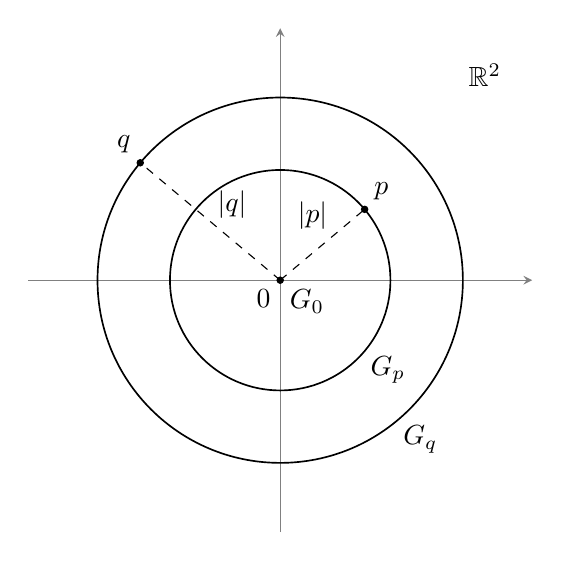
\begin{tikzpicture}[scale=0.8]
\draw[gray,->] (0,-4) -- (0,4);
\draw[gray,->] (-4,0) -- (4,0);
\draw (3.25,3.25) node {$\R^2$};
\draw[dashed] (0,0) -- (1.75*cos 40 , 1.75*sin 40) node[above right] {$p$};
\draw[fill] (1.75*cos 40 , 1.75*sin 40) circle[radius=0.05];
\draw (1.75*cos -40 , 1.75*sin -40) node[below right=-2pt] {$G_p$};
\draw (-0.1+0.8*cos 40 , 0.8*sin 40) node[above=3pt] {$|p|$};
\draw[dashed] (0,0) -- (2.9*cos 140 , 2.9*sin 140) node[above left] {$q$};
\draw[fill] (2.9*cos 140 , 2.9*sin 140) circle[radius=0.05];
\draw (2.9*cos -50 , 2.9*sin -50) node[below right=-2pt] {$G_q$};
\draw(1*cos 140 , 1*sin 140) node[above=4pt ] {$|q|$};
\draw[semithick] (0,0) circle [radius=1.75];
\draw[semithick] (0,0) circle [radius=2.9];
\draw[fill] (0,0) circle [radius=0.05] node[below right] {$G_0$};
\draw(0,0)  node[below left] {$0$};
\end{tikzpicture}
\end{center}
\ee

It should be intuitively clear from the definition that the orbits of two points are either disjoint or coincide. In fact, we have the following.

\bp
Let $\lacts \cl G\times M \to M$ be an action on $M$. Define a relation on $M$
\bse
p\sim q \ :\Leftrightarrow \ \exists \, g \in G : q = g \lacts p.
\ese
Then $\sim$ is an equivalence relation on $M$.
\ep

\bq
Let $p,q,r\in M$. We have
\begin{enumerate}[label=\roman*)]
\item $p\sim p$ since $p = e \lacts p$;
\item $p\sim q \Rightarrow q\sim p$ since, if $q =g \lacts p$, then
\bse
p = e \lacts p = (g^{-1}\bullet g) \lacts p = g^{-1}\lacts( g \lacts p)= g^{-1}\lacts q; 
\ese
\item $(p\sim q$ and $q\sim r) \Rightarrow p\sim r$ since, if $q =g_1 \lacts p$ and $r =g_2 \lacts q$, then
\bse
r = g_2 \lacts (g_1 \lacts p) = (g_1\bullet g_2)\lacts p.
\ese
\end{enumerate}
Therefore, $\sim$ is an equivalence relation on $M$.
\eq
The equivalence classes of $\sim$ are, by definition, the orbits.
\bd
Let $\lacts\cl G\times M\to M$ be an action on $M$. The \emph{orbit space} of $M$ is
\bse
M/G := M/\!\sim \,= \{G_p \mid p\in M\}.
\ese
\ed
\be
The orbit space of our previous $\SO(2,\R)$-action on $\R^2$ is the partition of $\R^2$ into concentric circles centred at the origin, plus the origin itself.
\ee
\bd
Let $\lacts\cl G\times M\to M$ be a $G$-action on $M$. The \emph{stabiliser}\index{stabiliser} of $p\in M$ is
\bse
S_p:=\{g\in G\mid g\lacts p = p\}.
\ese
\ed
Note that for each $p\in M$, the stabiliser $S_p$ is a subgroup of $G$.
\be
In our $\SO(2,\R)$ example, we have $S_p=\{\id_{\R^2}\}$ for $p\neq 0$ and $S_0=\SO(2,\R)$.
\ee
\bd
A left $G$-action $\lacts\cl G\times M\to M$ is said to be
\ben[label=\roman*)]
\item \emph{free} if for all $p\in M$, we have $S_p=\{e\}$;
\item \emph{transitive} if for all $p,q\in M$, there exists $g\in G$ such that $p=g\lacts p$.
\een
\ed

\be
The action $\lacts\cl G\times V \to V$ induced by a representation $R\cl G\to \GL(V)$ is never free since we always have $S_0=G$.
\ee

\be
Consider the action $\lacts\cl \mathrm{T}(n)\times \R^n\to \R^n$ of the $n$-dimensional translation group $\mathrm{T}(n)$ on $\R^n$. We have, rather trivially, $\mathrm{T}(n)_p=\R^n$ for every $p\in \R^n$.It is also easy to show that this action is free and transitive. 
\ee

\bp
Let $\lacts\cl G \times M \to M$ be a free action. Then
\bse
g_1 \lacts p = g_2 \lacts p \quad \Leftrightarrow \quad g_1 = g_2.
\ese
\ep
\bq
The $(\Leftarrow)$ direction is obvious. Suppose that there exist $p\in M$ and $g_1,g_2\in G$ such that $g_1 \lacts p = g_2 \lacts p$. Then
\bi{rCl}
g_1 \lacts p = g_2 \lacts p  &\quad  \Leftrightarrow \quad & g_2^{-1} \lacts (g_1 \lacts p) = g_2^{-1} \lacts(g_2 \lacts p)\\
& \Leftrightarrow & (g_2^{-1} \bullet g_1) \lacts p = (g_2^{-1}\bullet g_2) \lacts p\\
& \Leftrightarrow & (g_2^{-1}\bullet g_1)  \lacts p = (e\lacts p)\\
& \Leftrightarrow & (g_2^{-1}\bullet g_1)  \lacts p = p.
\ei
Hence $g_2^{-1}\bullet g_1\in S_p$, but since $\lacts$ is free we have $S_p=\{e\}$, and thus $g_1=g_2$.
\eq

\bp
If $\lacts\cl G \times M \to M$ is a free action, then
\bse
\forall \, p \in G :\ G_p \cong_{\mathrm{diff}} G.
\ese
\ep

\be
Define $\lacts\cl \SO(2,\R)\times \R^2\sm\{0\}\to \R^2\sm\{0\}$ to coincide with the action induced by the representation of $\SO(2,\R^2)$ on $\R^2$ for each non-zero point of $\R^2$. Then this action is free, since we have $S_p=\{\id_{\R^2}\}$ for $p\neq 0$, and the previous proposition implies
\bse
\forall \, p\in \R^2\sm\{0\} : \ \SO(2,\R)_p \cong_{\mathrm{diff}} \SO(2,\R) \cong_{\mathrm{diff}} S^1.
\ese
\ee


\subsection{Principal fibre bundles}

This is a good time to review our earlier section on bundles. We can specialize our definition of bundle to define a \emph{smooth bundle}, which is just a bundle $(E,\pi,M)$ where $E$ and $M$ are smooth manifolds and the projection $\pi\cl E\to M$ is smooth. Two smooth bundles $(E,\pi,M)$ and $(E',\pi',M')$ are isomorphic if there exist diffeomorphisms $u,f$ such that the following diagram commutes
\bse
\begin{tikzcd}
E \ar[dd,"\pi"'] \ar[rr,"u"] && E' \ar[dd,"\pi'"]\\
&&\\
M\ar[rr,"f"] && M'
\end{tikzcd}
\ese

\bd
Let $G$ be a Lie group. A smooth bundle $(E,\pi,M)$ is called a \emph{principal $G$-bundle}\index{principal bundle} if $E$ is equipped with a free right $G$-action and
\bse
\begin{tikzcd}
E \ar[d,"\pi"'] \\
M 
\end{tikzcd}
\ \ \cong_{\mathrm{bdl}}
\begin{tikzcd}
  E \ar[d,"\rho"]\\
  E/G
\end{tikzcd}
\ese
where $\rho$ is the quotient map, defined by sending each $p\in E$ to its equivalence class (i.e.\ orbit) in the orbit space $E/G$.
\ed
Observe that since the right action of $G$ on $E$ is free, for each $p\in E$ we have
\bse
\preim_\rho(G_p) = G_p \cong_{\mathrm{diff}} G.
\ese
We said at beginning that, roughly speaking, a principal bundle is a bundle whose fibre at each point is a Lie group. Note that the formal definition is that a principal $G$-bundle is a bundle which is isomorphic to a bundle whose fibres are the orbits under the right action of $G$, which are themselves isomorphic to $G$ since the action is free.

\br
A slight generalisation would be to consider smooth bundles $E\xrightarrow{\,\pi\,}M$ where $E$ is equipped with a right $G$-action which is free and transitive on each fibre of $E\xrightarrow{\,\pi\,}M$. The isomorphism in our definition enforces the fibre-wise transitivity since $G$ acts transitively on each $G_p$ by the definition of orbit.
\er

\be
\ben[label=\alph*)]
\item Let $M$ be a smooth manifold. Consider the space
\bse
L_pM := \{(e_1,\ldots,e_{\dim M})\mid e_1,\ldots,e_{\dim M} \text{ is a basis of }T_pM\} \cong_{\mathrm{vec}} \GL(\dim M,\R).
\ese
We know from linear algebra that the bases of a vector space are related to each other by invertible linear transformations. Hence, we have 
\bse
L_pM \cong_{\mathrm{vec}} \GL(\dim M,\R).
\ese
We define the frame bundle of $M$ as
\bse
LM := \coprod_{p\in M} L_pM
\ese
with the obvious projection map $\pi\cl LM \to M$ sending each basis $(e_1,\ldots,e_{\dim M})$ to the unique point $p\in M$ such that $(e_1,\ldots,e_{\dim M})$ is a basis of $T_pM$.
By proceeding similarly to the case of the tangent bundle, we can equip $LM$ with a smooth structure inherited from that of $M$. We then find
\bse
\dim LM = \dim M + \dim T_pM = \dim M + (\dim M)^2.
\ese
\item We would now like to make $LM \xrightarrow{\,\pi\,}M$ into a principal $\GL(\dim M,\R)$-bundle. We define a right $\GL(\dim M,\R)$-action on $LM$ by
\bse
(e_1,\ldots,e_{\dim M}) \racts g := (g^a_{\phantom{a}1}e_a,\ldots,g^a_{\phantom{a}\dim M}e_a),
\ese
where $g^a_{\phantom{a}b}$ are the components of the endomorphism $g\in \GL(\dim M, \R)$ with respect to the standard basis on $\R^n$. Note that if $(e_1,\ldots,e_{\dim M})\in L_pM$, we must also have $(e_1,\ldots,e_{\dim M}) \racts g\in L_pM$. This action is free since
\bse
(e_1,\ldots,e_{\dim M}) \racts g = (e_1,\ldots,e_{\dim M})  \Leftrightarrow  (g^a_{\phantom{a}1}e_a,\ldots,g^a_{\phantom{a}\dim M}e_a)= (e_1,\ldots,e_{\dim M}) 
\ese
and hence, by linear independence, $g^a_{\phantom{a}b}=\delta^a_b$, so $g=\id_{\R^n}$. Note that since all bases of each $T_pM$ are related by some $g\in \GL(\dim M,\R)$, $\racts$ is also fibre-wise transitive. 
\item We now have to show that
\bse
\begin{tikzcd}
LM \ar[d,"\pi"'] \\
M 
\end{tikzcd}
\ \ \cong_{\mathrm{bdl}}
\begin{tikzcd}
  LM \ar[d,"\rho"]\\
  LM \big/ \GL(\dim M,\R)
\end{tikzcd}
\ese
i.e.\ that there exist smooth maps $u$ and $f$ such that the diagram
\bse
\begin{tikzcd}
LM \ar[rr,shift left,"u"] \ar[dd,"\pi"']&& LM \ar[ll,shift left,"u^{-1}"]\ar[dd,"\rho"]\\
&&\\
M \ar[rr,shift left,"f"]&&  LM \big/ \GL(\dim M,\R)\ar[ll,shift left,"f^{-1}"]
\end{tikzcd}
\ese
commutes. We can simply choose $u=u^{-1}=\id_{LM}$, while we define $f$ as
\bi{rrCl}
f \cl & M & \to &  LM\big/ \GL(\dim M,\R)\\[2pt]
& p & \mapsto & \GL(\dim M,\R)_{(e_1,\ldots,e_{\dim M})},
\ei
where $(e_1,\ldots,e_{\dim M})$ is some basis of $T_pM$, i.e.\ $(e_1,\ldots,e_{\dim M})\in \preim_\pi(\{p\})$. Note that $f$ is well-defined since every basis of $T_pM$ gives rise to the same orbit in the orbit space $LM\big/\GL(\dim M,\R)$. Moreover, it is injective since
\bse
f(p)=f(p')\ \Leftrightarrow \ \GL(\dim M,\R)_{(e_1,\ldots,e_{\dim M})} = \GL(\dim M,\R)_{(e'_1,\ldots,e'_{\dim M})},
\ese
which is true only if $(e_1,\ldots,e_{\dim M})$ and $(e'_1,\ldots,e'_{\dim M})$ are basis of the same tangent space, so $p=p'$. It is clearly surjective since every orbit in $LM\big/ \GL(\dim M,\R)$ is the orbit of some basis of some tangent space $T_pM$ at some point $p\in M$. The inverse map is given explicitly by
\bi{rrCl}
f^{-1} \cl & LM\big/ \GL(\dim M,\R) & \to & M \\[2pt]
& \GL(\dim M,\R)_{(e_1,\ldots,e_{\dim M})} & \mapsto & \pi((e_1,\ldots,e_{\dim M})).
\ei
Finally, we have
\bse
(\rho\circ\id_{LM})(e_1,\ldots,e_{\dim M}) = \GL(\dim M,\R)_{(e_1,\ldots,e_{\dim M})} = (f\circ \pi)(e_1,\ldots,e_{\dim M})
\ese
and thus $LM\xrightarrow{\,\pi\,}M$ is a principal $G$-bundle, called the \emph{frame bundle}\index{frame bundle} of $M$.
\een
\ee

\br
A note to the careful reader. As we have just done in the previous example, in the following we will sometimes simply assume that certain maps are smooth, instead of rigorously proving it. 
\er

\subsection{Principal bundle morphisms}

Recall that a bundle morphism (also called simply a bundle map) between two bundles $(E,\pi,M)$ and $(E',\pi',M')$ is a pair of maps $(u,f)$ such that the diagram
\bse
\begin{tikzcd}
E \ar[dd,"\pi"'] \ar[rr,"u"] && E' \ar[dd,"\pi'"]\\
&&\\
M\ar[rr,"f"] && M'
\end{tikzcd}
\ese
commutes, that is, $f\circ \pi = \pi' \circ u$.
\bd
Let $(P,\pi,M)$ and $(Q,\pi',N)$ be principal $G$-bundles. A \emph{principal bundle morphism} from $(P,\pi,M)$ to $(Q,\pi',N)$ is a pair of smooth maps $(u,f)$ such that the diagram
\bse
\begin{tikzcd}
P \ar[rr,"u"]&& Q \\
&&\\
P \ar[uu,"{}\racts G"] \ar[dd,"\pi"'] \ar[rr,"u"] && Q\ar[uu,"{}\blacktriangleleft G"'] \ar[dd,"\pi'"]\\
&&\\
M\ar[rr,"f"] && N
\end{tikzcd}
\ese
commutes, that is for all $p\in P$ and $g\in G$, we have
\bi{rCl}
(f\circ \pi)(p)  & = & (\pi'\circ u)(p)\\
u(p\racts g) & = & u(p)\blacktriangleleft g.
\ei
\ed
Note that $P\xrightarrow{\quad \racts G \quad } P$ is a shorthand for the inclusion of $P$ into the product $P\times G$ followed by the right action $\racts$, i.e.\
\bse
\begin{tikzcd}
P \ar[rr,"\racts G"] && P
\end{tikzcd}
\ \quad =\quad \ 
\begin{tikzcd}
P \ar[rr,"i_1"] && P\times G \ar[rr,"\racts"] && P
\end{tikzcd}
\ese
and similarly for $Q\xrightarrow{\quad \blacktriangleleft G \quad } Q$.

\bd
A principal bundle morphism between two principal $G$-bundles is an \emph{isomorphism} (or \emph{diffeomorphism}) \emph{of principal bundles} if it is also a bundle isomorphism.
\ed

\br
Note that the passage from principal bundle morphism to principal bundle isomorphism does not require any extra condition involving the Lie group $G$. We will soon see that this is because the two bundles are both principal $G$-bundles. We can further generalise the notion of principal bundle morphism as follows.
\er

\bd
Let $(P,\pi,M)$ be a principal $G$-bundle, let $(Q,\pi',N)$ be a principal $H$-bundle, and let $\rho\cl G \to H$ be a Lie group homomorphism. A \emph{principal bundle morphism}\index{principal bundle morphism} from $(P,\pi,M)$ to $(Q,\pi',N)$ is a pair of smooth maps $(u,f)$ such that the diagram
\bse
\begin{tikzcd}
P \ar[rr,"u"]&& Q \\
&&\\
P\times G\ar[uu,"{}\racts "]  \ar[rr,"u\times \rho"]&& Q\times H \ar[uu,"{}\blacktriangleleft"'] \\
&&\\
P \ar[uu,"i_1"] \ar[dd,"\pi"'] \ar[rr,"u"] && Q\ar[uu,"i_1"'] \ar[dd,"\pi'"]\\
&&\\
M\ar[rr,"f"] && N
\end{tikzcd}
\ese
commutes, that is $f \circ \pi=\pi'\circ u $ and $u$ is a $\rho$-equivariant map
\bi{rCl}
\forall \, p\in P : \forall \, g \in G : \ u(p\racts g) & = & u(p)\blacktriangleleft \rho(g).
\ei
\ed

\bd
A principal bundle morphism between principal $G$-bundle and a principal $H$-bundle is an \emph{isomorphism} (or \emph{diffeomorphism}) \emph{of principal bundles}\index{isomorphism!of principal bundles} if it is also a bundle isomorphism and $\rho$ is a Lie group isomorphism.
\ed

\bl
Let $(P,\pi,M)$ and $(Q,\pi',M)$ be principal $G$-bundles over the same base manifold $M$. Then, any $u\cl P \to Q$ such that $(u,\id_M)$ is a principal bundle morphism is necessarily a diffeomorphism.
\bse
\begin{tikzcd}
P \ar[rr,"u"]&& Q \\
&&\\
P \ar[uu,"\racts G"] \ar[ddr,"\pi"'] \ar[rr,"u"] && Q\ar[uu,"\blacktriangleleft G"'] \ar[ddl,"\pi'"]\\
&&\\
 &M& 
\end{tikzcd}
\ese
\el

\bq
We already know that $u$ is smooth since $(u,\id_M)$ is assumed to be a principal bundle morphism. It remains to check that $u$ is bijective and its inverse is also smooth.
\ben[label=\roman*)]
\item Let $p_1,p_2\in P$ be such that $u(p_1)=u(p_2)$. Then
\bse
\pi(p_1) = \pi'(u(p_1)) = \pi'(u(p_2)) = \pi(p_2),
\ese
that is, $p_1$ and $p_2$ belong to the same fibre. As the action of $G$ on $P$ is fibre-wise transitive, there is a unique $g\in G$ such that $p_1 = p_2\racts g$. Then
\bse
u(p_1)  = u(p_2\racts g)  = u(p_2) \blacktriangleleft g = u(p_1) \blacktriangleleft g,
\ese
so $g\in S_{u(p_1)}$, but since $\blacktriangleleft$ is free, we have $g=e$ and thus
\bse
p_1 = p_2\racts e = p_2.
\ese
Therefore $u$ is injective.
\item Let $q\in Q$. Choose some $p\in \preim_\pi(\pi'(q))$. Then, we have
\bse
\pi'(u(p)) = \pi(p) = \pi'(q)
\ese
so that $u(p)$ and $q$ belong to the same fibre. Hence, there is a unique $g\in G$ such that $q = u(p)\blacktriangleleft g$. We thus have
\bse
q = u(p)\blacktriangleleft g = u(p\racts g)
\ese
and since $p\racts g\in P$, the map $u$ is surjective. 
\een
Hence, $u$ is a diffeomorphism.
\eq


\bd
A principal $G$-bundle $(P,\pi,M)$ if it is called \emph{trivial} if it is isomorphic as a principal $G$-bundle to the principal $G$-bundle $(M\times G,\pi_1,M)$ where $\pi_1$ is the projection onto the first component and the action is defined as
\bi{rrCl}
\blacktriangleleft \cl & (M\times G) \times G & \to &M\times G\\
& ((p,g),g') & \mapsto & (p,g)\blacktriangleleft g' := (p,g\bullet g').
\ei
\ed
By the previous lemma, a principal $G$-bundle $(P,\pi,M)$ is trivial if there exists a smooth map $u\cl P\to M\times G$ such that the following diagram commutes.
\bse
\begin{tikzcd}
P \ar[rr,"u"]&& M\times G \\
&&\\
P \ar[uu,"{}\racts G"] \ar[ddr,"\pi"'] \ar[rr,"u"] && M\times G\ar[uu,"{}\blacktriangleleft G"'] \ar[ddl,"\pi_1"]\\
&&\\
& M & 
\end{tikzcd}
\ese

The following result provides a necessary and sufficient criterion for when a principal bundle is trivial. Note that while we have used the lower case letter $p$ almost exclusively to denote points of the base manifold $M$, in the next proof we will use it to denote points of the total space $P$ instead.

\begin{theorem}
A principal $G$-bundle $(P,\pi,M)$ is trivial if, and only if, there exists a smooth section $\sigma\in\Gamma(P)$, that is, a smooth $\sigma \cl M \to P$ such that $\pi\circ \sigma = \id_M$.
\end{theorem}

\bq
\begin{itemize}
\item[$(\Rightarrow)$] Suppose that $(P,\pi,M)$ is trivial. Then there exists a diffeomorphism $u\cl P \to M\times G$ which make the following diagram commute
\bse
\begin{tikzcd}
P && \\
&&\\
P \ar[uu,"{}\racts G"] \ar[ddr,"\pi"']  && M \ar[ll,"u^{-1}"'] \times G\ar[ddl,"\pi_1"]\\
&&\\
& M & 
\end{tikzcd}
\ese
We can define
\bi{rrCl}
\sigma \cl & M & \to & P\\
& m & \mapsto & u^{-1}(m,e),
\ei
where $e$ is the identity of $G$. Then $\sigma$ is smooth since it is the composition of $u^{-1}$ with the map $p\mapsto (p,e)$, which are both smooth. We also have
\bse
(\pi\circ\sigma)(pm=\pi( u^{-1}(m,e)) = \pi_1 (m,e) = m,
\ese
for all $m\in M$, hence $\pi\circ\sigma=\id_M$ and thus $\sigma\in \Gamma(P)$.

\item[$(\Leftarrow)$] Suppose that there exists a smooth section $\sigma\cl M\to P$. Let $p\in P$ and consider the point $\sigma(\pi(p))\in P$. We have
\bse
\pi(\sigma(\pi(p))) = \id_M(\pi(p)) =\pi(p),
\ese
hence $\sigma(\pi(p))$ and $p$ belong to the same fibre, and thus there exists a unique group element in $G$ which links the two points via $\racts$. Since this element depends on both $\sigma$ and $p$, let us denote it by $\chi_\sigma(p)$. Then, $\chi_\sigma$ defines a function
\bi{rrCl}
\chi_\sigma \cl & P & \to & G\\
& p & \mapsto & \chi_\sigma(p)
\ei
and we can write
\bse
\forall \, p \in P : \ p = \sigma(\pi(p))\racts \chi_\sigma(p).
\ese
In particular, for any other $g\in G$ we have $p\racts g\in P$ and thus
\bse
p\racts g = \sigma(\pi(p\racts g))\racts \chi_\sigma(p\racts g) = \sigma(\pi(p))\racts \chi_\sigma(p\racts g),
\ese
where the second equality follows from the fact that the fibres of $P$ are precisely the orbits under the action of $G$.

On the other hand, we can act on the right with an arbitrary $g\in G$ directly to obtain  

\bse
p\racts g = (\sigma(\pi(p))\racts \chi_\sigma(p))\racts g = \sigma(\pi(p))\racts (\chi_\sigma(p)\bullet g).
\ese
Combining the last two equations yields
\bse
 \sigma(\pi(p))\racts \chi_\sigma(p\racts g) = \sigma(\pi(p))\racts (\chi_\sigma(p)\bullet g)
\ese
and hence
\bse
 \chi_\sigma(p\racts g) = (\chi_\sigma(p)\bullet g).
\ese
We can now define the map
\bi{rrCl}
u_\sigma \cl & P & \to & M \times G\\
& p & \mapsto & (\pi(p),\chi_\sigma(p)).
\ei
By our previous lemma, it suffices to show that $u_\sigma$ is a principal bundle map.

\bse
\begin{tikzcd}
P \ar[rr,"u_\sigma"]&& M\times G \\
&&\\
P \ar[uu,"{}\racts G"] \ar[ddr,"\pi"'] \ar[rr,"u_\sigma"] && M\times G\ar[uu,"{}\blacktriangleleft G"'] \ar[ddl,"\pi_1"]\\
&&\\
& M & 
\end{tikzcd}
\ese
By definition, we have
\bse
(\pi_1\circ u_\sigma)(p) = \pi_1 (\pi(p),\chi_\sigma(p))=\pi(p)
\ese
for all $p\in P$, so the lower triangle commutes. Moreover, we have
\bi{rCl}
u_\sigma(p\racts g) & = & (\pi(p\racts g),\chi_\sigma(p\racts g))\\
 & = & (\pi(p),\chi_\sigma(p)\bullet g))\\
 & = & (\pi(p),\chi_\sigma(p))\blacktriangleleft g\\
 & = & u_\sigma(p)\blacktriangleleft g
\ei
for all $p\in P$ and $g\in G$, so the upper square also commutes and hence $(P,\pi,M)$ is a trivial bundle. \qedhere
\end{itemize}
\eq

\be
The existence of a section on the frame bundle $LM$ can be reduced to the existence of $(\dim M)$ non-everywhere vanishing linearly independent vector fields on $M$. Since no such vector field exists on even-dimensional spheres, $LS^{2n}$ is always non-trivial.
\ee

















% \newpage

% \section{Associated fibre bundles}
% 
An associated fibre bundle is a fibre bundle which is associated (in a precise sense) to a principal $G$-bundle. Associated bundles are related to their underlying principal bundles in a way that models the transformation law for components under a change of basis.


\subsection{Associated fibre bundles}



\bd
Let $(P,\pi,M)$ be a principal $G$-bundle and let $F$ be a smooth manifold equipped with a left $G$-action $\lacts$. We define
\ben[label=\roman*)]
\item $P_F:=(P\times F)/{\sim_G}$, where $\sim_G$ is the equivalence relation
\bse
(p,f) \sim_G (p',f') \quad :\Leftrightarrow \quad \exists \, g\in G : \biggl\{ \ba{rcl} p' & = & p\racts g \\ f' & = & g^{-1} \lacts f \ea 
\ese
We denote the points of $P_F$ as $[p,f]$.
\item The map 
\bi{rrCl}
\pi_F\cl & P_F & \to & M\\
& [p,f] & \mapsto & \pi(p),
\ei
which is well-defined since, if $[p',f']=[p,f]$, then for some $g\in G$
\bse
\pi_F([p',f']) = \pi_F([p\racts g,g^{-1} \lacts f]):=\pi(p\racts g)=\pi(p)=:\pi_F([p,f]) .
\ese
\een
The \emph{associated bundle}\index{associated bundle} (to $(P,\pi,M)$, $F$ and $\lacts$) is the bundle $(P_F,\pi_F,M)$.
\ed

\be
Recall that the frame bundle $(LM,\pi,M)$ is a principal $\GL(d,\R)$-bundle, where $d=\dim M$, with right $G$-action $\racts\cl LM \times G \to LM$ given by
\bse
(e_1,\ldots,e_{d}) \racts g := (g^a_{\phantom{a}1}e_a,\ldots,g^a_{\phantom{a}d}e_a).
\ese
Let $F:= \R^{d}$ (as a smooth manifold) and define a left action
\bi{rrCl}
\lacts \cl & \GL(d,\R) \times \R^{d} & \to & \R^{d}\\
& (g,x) & \mapsto & g\lacts x,
\ei
where 
\bse
(g\lacts x)^a := g^a_{\phantom{a}b} x^b.
\ese
Then $(LM_{\R^d},\pi_{\R^d},\R^d)$ is the associated bundle. In fact, we have a bundle isomorphism

\bse
\begin{tikzcd}
LM_{\R^d} \ar[dd,"\pi_{\R^d}"'] \ar[rr,"u"] && TM\ar[dd,"\pi"] \\
&& \\
M \ar[rr,"\id_M"] && M
\end{tikzcd}
\ese
where $(TM,\pi,M)$ is the tangent bundle of $M$, and $u$ is defined as
\bi{rcCl}
u \cl & LM_{\R^d} & \to & TM\\
& [(e_1,\ldots,e_d),x] & \mapsto & x^ae_a.
\ei
The inverse map $u^{-1}\cl TM \to LM_{\R^d}$ works as follows. Given any $X\in TM$, pick any basis $(e_1,\ldots,e_d)$ of the tangent space at the point $\pi(X)\in M$, i.e.\ any element of $L_{\pi(X)}M$. Decompose $X$ as $x^ae_a$, with each $x^a\in \R$, and define
\bse
u^{-1}(X) := [(e_1,\ldots,e_d),x].
\ese
The map $u^{-1}$ is well-defined since, while the pair $((e_1,\ldots,e_d),x)\in LM\times \R^d$ clearly depends on the choice of basis, the equivalence class 
\bse
[(e_1,\ldots,e_d),x]\in LM_{\R^d}:=(LM\times \R^d)/{\sim_G}
\ese
does not. It includes all pairs $((e_1,\ldots,e_d)\racts g,g^{-1}\lacts x)$ for every $g\in \GL(d,\R)$, i.e.\ every choice of basis together with the ``right'' components $x\in \R^d$.
\ee

\br
Even though the associated bundle $(LM_{\R^d},\pi_{\R^d},\R^d)$ is isomorphic to the tangent bundle $(TM,\pi,M)$, note a subtle difference between the two. On the tangent bundle, the transformation law for a change of basis and the related transformation law for components are \emph{deduced} from the definitions by undergraduate linear algebra.

On the other hand, the transformation laws on $LM_{\R^d}$ were \emph{chosen} by us in its definition. We chose the Lie group $\GL(d,\R)$, the specific right action $\racts$ on $LM$, the space $\R^d$, and the specific left action on $\R^d$. It just happens that, with these choices, the resulting associated bundle is isomorphic to the tangent bundle. Of course, we have the freedom to make different choices and construct bundles which behave very differently from $TM$. 
\er

\be
Consider the principal $\GL(d,\R)$-bundle $(LM,\pi,M)$ again, with the same right action as before. This time we define
\bse
F:= (\R^d)^{\times p}\times({\R^d}^*)^{\times q} := \underbrace{\R^d\times\cdots\times\R^d}_{p \text{ times}}\times \underbrace{{\R^d}^*\times\cdots\times{\R^d}^*}_{q \text{ times}} 
\ese
with left $\GL(d,\R)$-action $\lacts\cl\GL(d,\R)\times F \to F$ given by
\bse
(g\lacts f)^{a_1\cdots a_p}_{\phantom{a_1\cdots a_p}b_1\cdots b_q} := g^{a_1}_{\phantom{a_1}\widetilde a_1} \cdots g^{a_p}_{\phantom{a_p}\widetilde a_p} (g^{-1})^{\widetilde b_1}_{\phantom{b_1}b_1}\cdots  (g^{-1})^{\widetilde b_q}_{\phantom{b_q}b_q} \, f^{\widetilde a_1\cdots \widetilde a_p}_{\phantom{a_1\cdots a_p}\widetilde b_1\cdots \widetilde b_q}.
%
% (g\lacts f)^{a_1\cdots a_p}_{\phantom{a_1\cdots a_p}b_1\cdots b_q} := g^{a_1}_{\phantom{a_1}r_1} \cdots g^{a_p}_{\phantom{a_p}r_p} (g^{-1})^{s_1}_{\phantom{s_1}b_1}\cdots  (g^{-1})^{s_q}_{\phantom{s_q}b_q} \, f^{r_1\cdots r_p}_{\phantom{r_1\cdots r_p}s_1\cdots s_q}.
%
% (g\lacts f)^{i_1\cdots i_p}_{\phantom{i_1\cdots i_p}j_1\cdots j_q} := g^{i_1}_{\phantom{i_1}\widetilde i_1} \cdots g^{i_p}_{\phantom{i_p}\widetilde i_p} g^{\widetilde j_1}_{\phantom{j_1}j_1}\cdots  g^{\widetilde j_q}_{\phantom{ j_q}j_q} \, f^{\widetilde i_1\cdots\widetilde  i_p}_{\phantom{i_1\cdots i_p}\widetilde j_1\cdots\widetilde  j_q}
\ese
Then, the associated bundle $(LM_F,\pi_F,M)$ thus constructed is isomorphic to $(T^p_qM,\pi,M)$, the $(p,q)$-tensor bundle on $M$.
\ee

Now for something new, consider the following.

\bd
Let $M$ be a smooth manifold and let $(LM,\pi,M)$ be its frame bundle, with right $\GL(d,\R)$-action as above. Let $F:= (\R^d)^{\times p}\times({\R^d}^*)^{\times q}$ and define a left $\GL(d,\R)$-action on $F$ by
\bse
(g\lacts f)^{a_1\cdots a_p}_{\phantom{a_1\cdots a_p}b_1\cdots b_q} := (\det g^{-1})^\omega\,g^{a_1}_{\phantom{a_1}\widetilde a_1} \cdots g^{a_p}_{\phantom{a_p}\widetilde a_p} (g^{-1})^{\widetilde b_1}_{\phantom{b_1}b_1}\cdots  (g^{-1})^{\widetilde b_q}_{\phantom{b_q}b_q} \, f^{\widetilde a_1\cdots \widetilde a_p}_{\phantom{a_1\cdots a_p}\widetilde b_1\cdots \widetilde b_q},
\ese
where $\omega\in \Z$. Then the associated bundle $(LM_F,\pi_F,M)$ is called the \emph{$(p,q)$-tensor $\omega$-density bundle} on $M$, and its sections are called \emph{$(p,q)$-tensor densities of weight}\index{tensor density} $\omega$.
\ed

\br
Some special cases include the following.
\ben[label=\roman*)]
\item If $\omega = 0$, we recover the $(p,q)$-tensor bundle on $M$.
\item If $F=\R$ (i.e.\ $p=q=0$), the left action reduces to
\bse
(g\lacts f) = (\det g^{-1})^\omega\, f,
\ese
which is the transformation law for a \emph{scalar density of weight $\omega$}.
\item If $\GL(d,\R)$ is restricted in such a way that we always have $(\det g^{-1})=1$, then tensor densities are indistinguishable from ordinary tensor fields. This is why you probably haven't met tensor densities in your special relativity course.
\een
\er

\be
Recall that if $B$ is a bilinear form on a $K$-vector space $V$, the determinant of $B$ is not independent from the choice of basis. Indeed, if $\{e_a\}$ and $\{e'_b:=g^a_{\phantom{a}b}e_a\}$ are both basis of $V$, where $g\in \GL(\dim V,K)$, then
\bse
(\det B)' = (\det g^{-1})^2\det B.
\ese
Once recast in the principal and associated bundle formalism, we find that the determinant of a bilinear form is a scalar density of weight $2$.
\ee

\subsection{Associated bundle morphisms}

\bd
Let $(P_F,\pi_F,M)$ to $(Q_F,\pi'_F,N)$ be the associated bundles (with the same fibre $F$) of two principal $G$-bundles $(P,\pi,M)$ and $(Q,\pi',N)$. An \emph{associated bundle map} between the associated bundles is a bundle map $(\widetilde u,v)$ between them such that for some $u$, the pair $(u,v)$ is a principal bundle map between the underlying principal $G$-bundles and  
\bse
\widetilde u([p,f]) := [u(p),f].
\ese
Equivalently, the following diagrams both commute.
\bse
\begin{tikzcd}
P_F \ar[dd,"\pi_F"'] \ar[rr,"\widetilde u"] && Q_F\ar[dd,"\pi_F'"]\\
&&\\
M \ar[rr,"v"] && N 
\end{tikzcd}
\qquad \quad
\begin{tikzcd}
P \ar[rr,"u"]&& Q \\
&&\\
P \ar[uu,"\racts G"] \ar[dd,"\pi"'] \ar[rr,"u"] && Q\ar[uu,"\blacktriangleleft G"'] \ar[dd,"\pi'"]\\
&&\\
M \ar[rr,"v"]&& N
\end{tikzcd}
\ese
\ed

\bd
An associated bundle map $(\widetilde u,v)$ is an \emph{associated bundle isomorphism}\index{isomorphism!of associated bundles} if $\widetilde u$ and $v$ are invertible and $(\widetilde u^{-1},v^{-1})$ is also an associated bundle map.
\ed

\br
Note that two associated $F$-fibre bundles may be isomorphic as bundles but not as associated bundles. In other words, there may exist a bundle isomorphism between them, but there may not exist any bundle isomorphism between them which can be written as in the definition for some principal bundle isomorphism between the underlying principal bundles. 
\er

\noindent Recall that an $F$-fibre bundle $(E,\pi,M)$ is called trivial if there exists a bundle isomorphism
\bse
\begin{tikzcd}
F \ar[rr] && E\ar[ddr,"\pi"]\ar[rr,"u"] && M\times F \ar[ddl,"\pi_1"]\\
&&&&\\
&&& M &
\end{tikzcd}
\ese
while a principal $G$-bundle is called trivial if there exists a principal bundle isomorphism
\bse
\begin{tikzcd}
P \ar[rr,"u"]&& M\times G \\
&&\\
P \ar[uu,"\racts G"] \ar[ddr,"\pi"'] \ar[rr,"u"] && M\times G\ar[uu,"\blacktriangleleft G"'] \ar[ddl,"\pi_1"]\\
&&\\
& M & 
\end{tikzcd}
\ese

\bd
An associated bundle $(P_F,\pi_F,M)$ is called \emph{trivial} if the underlying principal $G$-bundle $(P,\pi,M)$ is trivial.
\ed

\bp
A trivial associated bundle is a trivial fibre bundle.
\ep
Note that the converse does not hold. An associated bundle can be trivial as a fibre bundle but not as an associated bundle, i.e.\ the underlying principal fibre bundle need not be trivial simply because the associated bundle is trivial as a fibre bundle.

% \bt
% Let $(P_F,\pi_F,M)$ be an associated bundle. There exists a bijection between sections $\sigma\cl M \to P_F$ and functions $\phi\cl P\to F$. 
% \et

\bd
Let $H$ be a closed Lie subgroup of $G$. Let $(P,\pi,M)$ be a principal $H$-bundle and $(Q,\pi',M)$ a principal $G$-bundle. If there exists a principal bundle map from $(P,\pi,M)$ to $(Q,\pi',M)$, i.e.\ a smooth bundle map which is equivariant with respect to the inclusion of $H$ into $G$, then $(P,\pi,M)$ is called an \emph{$H$-restriction} of $(Q,\pi',M)$, while $(Q,\pi',M)$ is called a \emph{$G$-extension} of $(P,\pi,M)$.  
\ed

\bt
Let $H$ be a closed Lie subgroup of $G$.
\ben[label=\roman*)]
\item Any principal $H$-bundle can be extended to a principal $G$-bundle.
\item A principal $G$-bundle $(P,\pi,M)$ can be restricted to a principal $H$-bundle if, and only if, the bundle $(P/H,\pi',M)$ has a section.
\een
\et

\be
\ben[label=\roman*)]
\item The bundle $(LM/\SO(d),\pi,M)$ always has a section, and since $\SO(d)$ is a closed Lie subgroup of $\GL(d,\R)$, the frame bundle can be restricted to a principal $\SO(d)$-bundle. This is related to the fact that any manifold can be equipped with a Riemannian metric.   
\item The bundle $(LM/\SO(1,d-1),\pi,M)$ may or may not have a section.  For example, the bundle $(LS^2/\SO(1,1),\pi,S^2)$ does not admit any section, and hence we cannot restrict $(LS^2/\SO(1,1),\pi,S^2)$ to a principal $\SO(1,1)$-bundle, even though $\SO(1,1)$ is a closed Lie subgroup of $\GL(2,\R)$. This is related to the fact that the $2$-sphere cannot be equipped with a Lorentzian metric.
\een
\ee


















% \newpage

% \section{Connections and connection 1-forms}
% 
In elementary courses on differential geometry or general relativity, the notions of connection, parallel transport and covariant derivative are often confused with one another. Sometimes, the terms are even used as synonyms. If you have seen any of that before, it is probably best to forget about it for the time being.

What a connection really is, is just additional structure on a principal bundle consisting is a ``smooth'' assignment of a particular vector space at each point of the base manifold compatible with the right action of the Lie group on the principal bundle. Such an assignment is, in fact, equivalent to a certain Lie-algebra-valued one-form on the principal bundle, as we will discuss below. Later, we will see that a connection on a principal bundle induces a parallel transport map on the principal bundle, which in turn induces a parallel transport map on any of its associated bundles. If the fibres of the associated bundle carry a vector space structure, then the parallel transport can be used to define a covariant derivative on the associated bundle. 

Hence the conceptual sequence ``connection, parallel transport covariant derivative'' is in decreasing order of generality, and it should be clear that treating these terms as synonyms will inevitably lead to confusion. We will now discuss the first of these in some detail.



\subsection{Connections on a principal bundle}

Let $(P,\pi,M)$ be a principal $G$-bundle. Recall that every element of $A\in T_eG$ gives rise to a left invariant vector field on $G$ which we denoted by $X^A$. However, we will now reserve this notation for a vector field on $P$ instead. Given $A\in T_eG$, we define $X^A\in\Gamma(TP)$ by
\bi{rrCl}
X^A_p\cl & \mathcal{C}^\infty(P) &\xrightarrow{\sim} & \R \\
& f & \mapsto & [f(p\racts \exp(tA))]'(0),
\ei
where the derivative is to be taken with respect to $t$. We also define the maps
\bi{rrCl}
i_p\cl & T_eG & \to & T_pP\\
& A & \mapsto & X^A_p,
\ei
which can be shown to be a Lie algebra homomorphism.

\bd
Let $(P,\pi,M)$ be a principal bundle and let $p\in P$. The \emph{vertical subspace}\index{vertical subspace} at $p$ is the vector subspace of $T_pP$ given by
\bi{rCl}
V_pP  & := & \ker((\pi_*)_p)\\
& = & \{X_p\in T_pP \mid (\pi_*)_p(X_p)=0\}.
\ei
\ed

\bl
For all $A\in T_eG$ and $p\in P$, we have $X^A_p\in V_pP$.
\el

\bq
Since the action of $G$ simply permutes the elements within each fibre, we have
\bse
\pi(p) = \pi(p\racts \exp(tA)),
\ese
for any $t$. Let $f\in \mathcal{C}^\infty(M)$ be arbitrary. Then
\bi{rCl}
(\pi_*)_pX_p^A(f) & = & X_p^A(f\circ \pi)\\
& = & [(f\circ \pi)(p\racts \exp(tA))]'(0)\\
& = & [f(\pi(p))]'(0)\\
& = & 0,
\ei
since $f(\pi(p))$ is constant. Hence $X_p^A\in V_pP$. Alternatively, one can also argue that $(\pi_*)_pX^A_p$ is the tangent vector to a constant curve on $M$.
\eq

In particular, the map $i_p\cl T_eG\xrightarrow{\sim} V_pP$ is now a bijection.
The idea of a connection is to make a choice of how to ``connect'' the individual points in ``neighbouring'' fibres in a principal fibre bundle.

\bd
Let $(P,\pi,M)$ be a principal bundle and let $p\in P$. A \emph{horizontal subspace}\index{horizontal subspace} at $p$ a vector subspace $H_pP$ of $T_pP$ which is complementary to $V_pP$, i.e.\
\bi{rCl}
 T_pP = H_pP \oplus V_pP .
\ei
\ed

The choice of horizontal space at $p\in P$ is not unique. However, once a choice is made, there is a unique decomposition of each $X_p\in T_pP$ as
\bse
X_p=\hor(X_p)+\ver(X_p),
\ese
with $\hor(X_p)\in H_pP$ and $\ver(X_p)\in V_pP$.

\bd
A \emph{connection}\index{connection} on a principal $G$-bundle $(P,\pi,M)$ is a choice of horizontal space at each $p\in P$ such that
\ben[label=\roman*)]
\item For all $g\in G$, $p\in P$ and $X_p\in H_pP$, we have
\bse
(\racts g)_* X_p  \in H_{p\racts g}P,
\ese
where $(\racts g)_*$ is the push-forward of the map $(-\racts g)\cl P \to P$ and it is a bijection. We can also write this condition more concisely as
\bse
(\racts g)_* (H_pP) = H_{p\racts g}P.
\ese
\item For every smooth $X\in \Gamma(TP)$, the two summands in the unique decomposition
\bse
X|_p = \hor(X|_p)+\ver(X|_p)
\ese
at each $p\in P$, extend to smooth $\hor(X),\ver(X)\in\Gamma(TM)$.
\een
\ed
The definition formalises the idea that the assignment of an $H_pP$ to each $p\in P$ should be ``smooth'' within each fibre (i) as well as between different fibres (ii).  

\br
For each $X_p\in T_pP$, both $\hor(X_p)$ and $\ver(X_p)$ depend on the choice of $H_pP$. 
\er

\subsection{Connection one-forms}

Technically, the choice of a horizontal subspace $H_pP$ at each $p\in P$ providing a connection is conveniently encoded in the thus induced Lie-algebra-valued one-form
\bi{rrCl}
\omega_p \cl & T_pP & \xrightarrow{\sim} & T_eG\\
& X_p & \mapsto & \omega_p(X_p):=  i_p^{-1}(\ver(X_p))
\ei

\bd
The map $\omega\cl p\to \omega_p$ sending each $p\in P$ to the $T_eG$-valued one-form $\omega_p$ is called the \emph{connection one-form} with respect to the connection.
\ed

\br
We have seen how to produce a one-form from a choice of horizontal spaces (i.e.\ a connection). The choice of horizontal spaces can be recovered from $\omega$ by
\bse
H_pP = \ker (\omega_p).
\ese
\er

Of course, not every (Lie-algebra-valued) one-form on $P$ is such that $\ker(\omega_p)$ gives a connection on the principal bundle. What we would now like to do is to study some crucial properties of $\omega$. We will then elevate these properties to a definition of connection one-form absent a connection, so that we may re-define the notion of connection in terms of a connection one-form.

\bl
For all $p\in P$, $g\in G$ and $A\in T_eG$, we have
\bse
(\racts g)_*X^A_p = X^{(\Ad_{g^{-1}})_*A}_{p\racts g}.
\ese
\el

\bq
Let $f\in \mathcal{C}^\infty(P)$ be arbitrary. We have
\bi{rCl}
(\racts g)_*X^A_p (f) & = & X^A_p (f\circ (-\racts g))\\
& = & [f(p \racts \exp(tA)\racts g)]'(0)\\
& = & [f(p \racts g \racts g^{-1}\racts \exp(tA)\racts g)]'(0)\\
& = & [f(p \racts g \racts (g^{-1}\bullet \exp(tA)\bullet g)]'(0)\\
& = & [f(p \racts g \racts \Ad_{g^{-1}}(\exp(tA))]'(0)\\
& = & [f(p \racts g \racts \exp(t(\Ad_{g^{-1}})_*A)]'(0)\\
& = & X^{(\Ad_{g^{-1}})_*A}_{p\racts g} (f),
\ei
which is what we wanted.
\eq

\bt
A connection one-form $\omega$ with respect to a connection satisfies
\ben[label=\alph*)]
\item For all $p\in P$, we have $\omega_p(X^A_p)=A$, that is  $\omega_p\circ i_p = \id_{T_eG}$.
\bse
\begin{tikzcd}
T_eG \ar[rr,"i_p"] \ar[ddrr,"\id_{T_eG}"']&& V_pP \ar[dd,"\omega_p|_{V_pP}\phantom{nn}"]\\
&&\\
&& T_eG
\end{tikzcd}
\ese
\item $((\racts g)^*\omega)|_p (X_p)= (\Ad_{g^{-1}})_*(\omega_p(X_p))$
\bse
\begin{tikzcd}
T_pP \ar[rr,"\omega_p"] \ar[ddrr,"((\racts g)^*\omega)|_p "']&& T_eG \ar[dd,"(\Ad_{g^{-1}})_*"]\\
&&\\
&& T_eG
\end{tikzcd}
\ese
\item $\omega$ is a smooth one-form.
\een
\et

\bq
\ben[label=\alph*)]
\item Since $X^A_p\in V_pP$, by definition of $\omega$ we have
\bse
\omega_p(X^A_p):=i_p^{-1}(\ver(X^A_p))=i_p^{-1}(X^A_p)=A.
\ese
\item First observe that the left hand side is linear in $X_p$. Consider the two cases
\ben[label=b.\arabic*)]
\item Suppose that $X_p\in V_pP$. Then $X_p=X_p^A$ for some $A\in T_eG$. Hence
\bi{rCl}
((\racts g)^*\omega)|_p (X^A_p) & = & \omega_{p\racts g}((\racts g)_*X^A_p)\\
& = & \omega_{p\racts g}\Bigl(X^{(\Ad_{g^{-1}})_*A}_{p\racts g}\Bigr)\\
& = & (\Ad_{g^{-1}})_*A\\
& = & (\Ad_{g^{-1}})_*(\omega_p(X^A_p))
\ei
\item Suppose now that $X_p\in H_pP=\ker(\omega_p)$. Then
\begin{equation*}
((\racts g)^*\omega)|_p (X_p) =  \omega_{p\racts g}((\racts g)_*X_p) = 0
\end{equation*}
since $(\racts g)_*X_p\in H_{p\racts g}P=\ker(\omega_{p\racts g})$. 
\een
Let $X_p\in T_pP$. We have
\bi{rCl}
((\racts g)^*\omega)|_p (X_p) & = & ((\racts g)^*\omega)|_p (\ver(X_p)+\hor(X_p)) \\
& = & ((\racts g)^*\omega)|_p (\ver(X_p)) +((\racts g)^*\omega)|_p (\hor(X_p)) \\
& = & (\Ad_{g^{-1}})_*(\omega_p(\ver(X_p))) + 0 \\
& = & (\Ad_{g^{-1}})_*(\omega_p(\ver(X_p))) +(\Ad_{g^{-1}})_*(\omega_p(\hor(X_p)))\\
& = & (\Ad_{g^{-1}})_*(\omega_p(\ver(X_p)+\hor(X_p)))\\
& = & (\Ad_{g^{-1}})_*(\omega_p(X_p))
\ei
\item We have $\omega=i^{-1}\circ\ver$ and both $i^{-1}$ and $\ver$ are smooth.\qedhere
\een
\eq

















% \newpage

% \section{Local representations of a connection on the base manifold: Yang-Mills fields}
% We have seen how to associate a connection one-form to a connection, i.e.\ a certain Lie-algebra-valued one-form to a smooth choice of horizontal spaces on the principal bundle. We will now study how we can express this connection one-form locally on the base manifold of the principal bundle. 

\subsection{Yang-Mills fields and local representations}

Recall that a connection one-form on a principal bundle $(P,\pi,M)$ is a smooth Lie-algebra-valued one-form, i.e.\ a smooth map
\bse
\omega\cl \Gamma(TP) \xrightarrow{\sim} T_eG
\ese
which ``behaves like a one-form'', in the sense that it is $\R$-linear and satisfies the Leibniz rule, and such that, in addition, for all $A\in T_eG$, $g\in G$ and $X\in \Gamma(TP)$, we have
\ben[label=\roman*)]
\item $\omega(X^A)=A$;
\item $((\racts g)^*\omega)(X)=(\Ad_{g^{-1}})_*(\omega(X))$.
\een
If the pair $(u,f)$ is a principal bundle automorphism of $(P,\pi,M)$, i.e.\ if the diagram
\bse
\begin{tikzcd}
P \ar[rr,"u"]&& P \\
&&\\
P\ar[rr,"u"] \ar[dd,"\pi"'] \ar[uu,"\racts G"] && P\ar[dd,"\pi"] \ar[uu,"\racts G"'] \\
&& \\
M \ar[rr,"f"]&& M
\end{tikzcd}
\ese
commutes, we should be able to pull a connection one-form $\omega$ on $P$ back to another connection one-form $u^*\omega$ on $P$.
\bse
\begin{tikzcd}
\Gamma(TP)\ar[rr,"\omega"]   && T_eG \\
&& \\
\Gamma(TP) \ar[uu,"u"] \ar[rruu,"u^*\omega"']&&
\end{tikzcd}
\ese
Recall that for a one-form $\omega\cl \Gamma(TN)\xrightarrow{\sim}\mathcal{C}^\infty(N)$, we defined
\bi{rrCl}
\Phi^*(\omega)\cl & \Gamma(TM) & \xrightarrow{\sim} & \mathcal{C}^\infty(M)\\
& X & \mapsto & \omega(\Phi_*(X))\circ \phi
\ei
for any diffeomorphism $\phi\cl M \to N$. One might be worried about whether this and similar definitions apply to Lie-algebra-valued one-forms but, in fact, they do. In our case, even though $\omega$ lands in $T_eG$, its domain is still $\Gamma(TP)$ and if $u\cl P\to P$ is a diffeomorphism of $P$, then $u_*X\in \Gamma(TP)$ and so
\bse
u^*\omega\cl X \mapsto (u^*\omega)(X):=\omega(u_*(X))\circ u
\ese
is again a Lie-algebra-valued one-form. Note that we will no longer distinguish notationally between the push-forward of tangent vectors and of vector fields.

In practice, e.g. for calculational purposes, one may wish to restrict attention to some open subset $U\se M$. Let $\sigma\cl U\to P$ be a local section of $P$, i.e.\ $\pi\circ \sigma = \id_U$.
\bse
\begin{tikzcd}
P\\
\\
P\ar[dd,"\pi"']\ar[uu,"\racts G"]\\
\\
U\ar[uu,bend right=60,"\sigma"']
\end{tikzcd}
\ese
\bd
Given a connection one-form $\omega$ on $P$, such a local section $\sigma$ induces
\ben[label=\roman*)]
\item a \emph{Yang-Mills field} $\omega^U\cl \Gamma(TU) \xrightarrow{\sim} T_eG$ given by
\bse
\omega^U:= \sigma^* \omega;
\ese
\item a \emph{local trivialisation} of the principal bundle $P$, i.e.\ a map
\bi{rrCl}
h\cl & U\times G & \to & P\\
& (m,g)& \mapsto & \sigma(m)\racts g;
\ei
\item a \emph{local representation}\index{connection!local representation} of $\omega$ on $U$ by
\bse
h^* \omega \cl \Gamma(T(U\times G))  \xrightarrow{\sim} T_eG.
\ese
\een
\ed
Note that, at each point $(m,g)\in U\times G$, we have
\bse
T_{(m,g)}(U\times G) \cong_{\mathrm{Lie \, alg}} T_mU\oplus T_gG.
\ese
\br
Both the Yang-Mills field $\omega^U$ and the local representation $h^*\omega$ encode the information carried by $\omega$ locally on $U$. Since $h^*\omega$ involves $U\times G$ while $\omega^U$ doesn't, one might guess that $h^*\omega$ gives a more ``accurate'' picture of $\omega$ on $U$ than the Yang-Mills field. But in fact, this is not the case. They both contain the same amount of local information about the connection one-form $\omega$.
\er

\subsection{The Maurer-Cartan form}

Th relation between the Yang-Mills field and the local representation is provided by the following result.

\begin{theorem}\label{thm:maurer-cartan}
For all $v\in T_mU$ and $\gamma \in T_gG$, we have
\bse
(h^*\omega)_{(m,g)}(v,\gamma) = (\Ad_{g^{-1}})_*(\omega^U(v))+\Xi_g(\gamma),
\ese
where $\Xi_g$ is the Maurer-Cartan form\index{Maurer-Cartan form}
\bi{rrCl}
\Xi_g \cl & T_gG & \xrightarrow{\sim} & T_eG\\
& L^A_g &\mapsto & A.
\ei
\end{theorem}

\br
Note that we have represented a generic element of $T_gG$ as $L^A_g$. This is due to the following. Recall that the left translation map $\ell_g\cl G \to G$ is a diffeomorphism of $G$. As such, its push-forward at any point is a linear isomorphism. In particular, we have
\bse
((\ell_g)_*)_e \cl T_eG \xrightarrow{\sim} T_gG,
\ese
that is, the tangent space at any point $g\in G$ can be canonically identified with the tangent space at the identity. Hence, we can write any element of $T_gG$ as
\bse
L^A_g := ((\ell_g)_*)_e (A)
\ese
for some $A\in T_eG$.
\er

Let us consider some specific examples.

\be
Any chart $(U,x)$ of a smooth manifold $M$ induces a local section $\sigma\cl U\to LM$ of the frame bundle of $M$ by
\bse
\sigma(m):=\biggl(\tvb{x}{1}{m},\ldots,\tvb{x}{\dim M}{m\,} \biggr)\in L_mM.
\ese
Since $\GL(\dim M,\R)$ can be identified with an open subset of $\R^{(\dim M)^2}$, we have
\bse
T_e\GL(\dim M,\R)\cong_{\mathrm{Lie\, alg}} \R^{(\dim M)^2},
\ese
where $\R^{(\dim M)^2}$ is understood as the algebra of $\dim M \times \dim M$ square matrices, with bracket induced by matrix multiplication. 
In fact, this holds for any open subset of a vector space, when considered as a smooth manifold. A connection one-form 
\bse
\omega\cl \Gamma(LM)\xrightarrow{\sim}T_e\GL(\dim M,\R)
\ese
can thus be given in terms of $(\dim M)^2$ functions 
\bse
\omega^i_{\phantom{i}j}\cl \Gamma(LM)\xrightarrow{\sim}\R, \qquad 1\leq i,j\leq \dim M.
\ese
The associated Yang-Mills field $\omega^U:=\sigma^*\omega$ is, at each point $m\in U$, a Lie-algebra-valued one-form on the vector space $T_mU$. By using the co-ordinate induced basis and its dual basis, we can express $(\omega^U)_m$ in terms of components as
\bse
(\omega^U)_m=\omega^U_\mu(m)\,(\d x^\mu)_m,
\ese
where $1\leq \mu \leq \dim M$ and
\bse
\omega^U_\mu(m):=(\omega^U)_m\biggl(\tvb{x}{\mu}{m}\biggr).
\ese
Since $(\omega^U)_m\cl T_mU\xrightarrow{\sim}T_eG$, we have $\omega^U_\mu\cl U \to T_eG$. Hence, by employing he same isomorphism as above, we can identify each $\omega^U_\mu(m)$ with a square $\dim M \times \dim M$ matrix and define the symbol
\bse
\Gamma^i_{\phantom{i}j\mu} (m):= (\omega^U(m))^i_{\phantom{i}j\mu}:= (\omega^U_\mu(m))^i_{\phantom{i}j},
\ese
usually referred to as the \emph{Christoffel symbol}\index{Christoffel symbol}. The middle term is just an alternative notation for the right-most side. Note that, even though all three indices $i$, $j$, $\mu$ run from $1$ to $\dim M$, the numbers $\Gamma^i_{\phantom{i}j\mu} (m)$ do not constitute the components of a $(1,2)$-tensor on $U$. Only the $\mu$ index transforms as a one-form component index, i.e.\
\bse
((g\lacts \omega^U(m))^i_{\phantom{i}j})_\mu = (g^{-1})^{\nu}_{\phantom{\mu}}(\omega^U(m))^i_{\phantom{i}j_\nu}
\ese
for $g\in \GL(\dim M,\R)$, while the $i$, $j$ indices simply label different one-forms, $(\dim M)^2$ in total. 
\ee

Note that the Maurer-Cartan form appearing in \Cref{thm:maurer-cartan} only depends on the Lie group (and its Lie algebra), not on the principal bundle $P$ or the restriction $U\se M$. In the following example, we will go through the explicit calculation of the Maurer-Cartan form of the Lie group $\GL(d,\R)$.

\be
Let $(\GL^+(d,\R),x)$ be a chart on $\GL(d,\R)$, where $\GL^+(d,\R)$ denotes an open subset of $\GL(d,\R)$ containing the identity $\id_{\R^d}$, and let $x^i_{\phantom{i}j}\cl \GL^+(d,\R)\to \R$ denote the corresponding co-ordinate functions
\bse
\begin{tikzcd}
\GL^+(d,\R) \ar[ddrr,"x^i_{\phantom{i}j}"']\ar[rr,"x"]&& x(\GL^+(d,\R))\se \R^{d^2} \ar[dd,"\proj^i_{\phantom{i}j}"]\\
&&\\
&& \R
\end{tikzcd}
\ese
so that $x^i_{\phantom{i}j}(g):=g^i_{\phantom{i}j}$. Recall that the co-ordinate functions are smooth maps on the chart domain, i.e.\ we have $x^i_{\phantom{i}j}\in \mathcal{C}^\infty(\GL^+(d,\R))$. Also recall that to each $A\in T_{\id_{\R^d}}\GL(d,\R)$ there is associated a left-invariant vector field
\bse
L^A\cl \mathcal{C}^\infty(\GL^+(d,\R))\xrightarrow{\sim} \mathcal{C}^\infty(\GL^+(d,\R))
\ese
which, at each point $g\in \GL(d,\R)$, is the tangent vector to the curve
\bse
\gamma^A(t) := g\bullet \exp(tA).
\ese
Consider the action of $L^A$ on the co-ordinate functions:
\bi{rCl}
(L^Ax^i_{\phantom{i}j})(g) & = & [x^i_{\phantom{i}j}(g\bullet \exp(tA))]'(0)\\
& = & [x^i_{\phantom{i}j}(g\bullet\e^{tA})]'(0)\\
& = & (g^i_{\phantom{i}k}(\e^{tA})^k_{\phantom{k}j})'(0)\\
& = & g^i_{\phantom{i}k}A^k_{\phantom{k}j},
\ei
where we have used the fact that for a matrix Lie group, the exponential map is just the ordinary exponential 
\bse
\exp(A) = \e^A := \sum_{n=0}^\infty \frac{1}{n!}A^n.
\ese
Hence, we can write
\bse
L^A|_g = g^i_{\phantom{i}k}A^k_{\phantom{k}j} \tvb{x^i_{\phantom{i}j}}{}{g}
\ese
from which we can read-off the Maurer-Cartan form of $\GL(d,\R)$
\bse
(\Xi_g)^i_{\phantom{i}j}:= (g^{-1})^i_{\phantom{i}k} (\d x^k_{\phantom{k}j})_g.
\ese
Indeed, we can quickly check that
\bi{rCl}
(\Xi_g)^i_{\phantom{i}j}(L^A) & = & (g^{-1})^i_{\phantom{i}k} (\d x^k_{\phantom{k}j})_g\biggl(  g^p_{\phantom{p}r}A^r_{\phantom{r}q} \tvb{x^p_{\phantom{p}q}}{}{g\,}\biggr) \\
& = & (g^{-1})^i_{\phantom{i}k}g^p_{\phantom{p}r}A^r_{\phantom{r}q}\delta^k_p\delta^q_j\\
& = & (g^{-1})^i_{\phantom{i}p}g^p_{\phantom{p}r}A^r_{\phantom{r}j}\\
& = & \delta^i_r A^r_{\phantom{r}j}\\
& = &  A^i_{\phantom{i}j}.
\ei
\ee

\subsection{The gauge map}

In physics, we are often prompted to write down a Yang-Mills field because we have local information about a connection. We can then try to reconstruct the global connection by glueing the Yang-Mills fields on several open subsets of our manifold. 
\bse
\begin{tikzcd}
&P \ar[ddl,"\pi"'] \ar[ddr,"\pi"] &\\
&&\\
U_1 \ar[uur,bend left=80,"\sigma_1"]&& U_2 \ar[uul,bend right=80,"\sigma_2"']
\end{tikzcd}
\ese
Suppose, for instance, that we have two open subsets $U_1,U_2\se M$ and consider the Yang-Mills fields associated to two local connections $\sigma_1,\sigma_2$. If $\omega^{U_1}$ and $\omega^{U_2}$ are both local versions of a unique connection one-form, then is $U_1\cap U_2\neq \varnothing$, the Yang-Mills fields $\omega^{U_1}$ and $\omega^{U_2}$ should satisfy some compatibility condition on $U_1\cap U_2$.

\bd
Within the above set-up, the \emph{gauge map}\index{gauge map} is the map
\bse
\Omega \cl U_1\cap U_2 \to G
\ese
where, for each $m\in U_1\cap U_2$, the Lie group element $\Omega(m)\in G$ satisfies
\bse
\sigma_2(m) = \sigma_1(m)\racts \Omega(m).
\ese
\ed
Note that since the $G$-action $\racts$ on $P$ is free, for each $m$ there exists a unique $\Omega(m)$ satisfying the above condition, and hence the gauge map $\Omega$ is well-defined.

\begin{theorem}
Under the above assumptions, we have
\bse
(\omega^{U_2})_m = (\Ad_{\Omega^{-1}(m)})_*( \omega^{U_1})+(\Omega^*\Xi_g)_m.
\ese
\end{theorem}

\be
Consider again the frame bundle $LM$ of some manifold $M$. Let us evaluate explicitly the pull-back along $\Omega$ of the Maurer-Cartan form. Since $\Xi_g\cl T_gG \to T_eG$ and $\Omega\cl U_1\cap U_2\to T_eG$, we have $\Omega^*\Xi_g\cl T(U_1\cap U_2)\to T_eG$. Let $x$ be a chart map near the point $m\in U_1\cap U_2$. We have
\bi{rCl}
((\Omega^*\Xi_g)_m)^i_{\phantom{i}j} \biggl(\tvb{x}{\mu}{m\,}\biggr) & = & (\Xi_{\Omega(m)})^i_{\phantom{i}j} \biggl(\Omega_*\tvb{x}{\mu}{m\,}\biggr) \\
 & = & (\Omega(m)^{-1})^i_{\phantom{i}k} (\d \widetilde x^k_{\phantom{k}j})_{\Omega(m)}\biggl(\Omega_*\tvb{x}{\mu}{m\,}\biggr) \\
 & = & (\Omega(m)^{-1})^i_{\phantom{i}k} \biggl(\Omega_*\tvb{x}{\mu}{m\,}\biggr) (\widetilde x^k_{\phantom{k}j})  \\
 & = & (\Omega(m)^{-1})^i_{\phantom{i}k} \tvb{x}{\mu}{m} (\widetilde x^k_{\phantom{k}j}\circ \Omega)  \\
 & = & (\Omega(m)^{-1})^i_{\phantom{i}k} \tvb{x}{\mu}{m} (\Omega(m))^k_{\phantom{k}j} .
\ei
hence, we can write
\bi{rCl}
((\Omega^*\Xi_g)_m)^i_{\phantom{i}j} & = & (\Omega(m)^{-1})^i_{\phantom{i}k} \tvb{x}{\mu}{m} (\Omega(m))^k_{\phantom{k}j} \d x^\mu \\
&=:& (\bm{\Omega}^{-1}\d \bm{\Omega})^i_{\phantom{i}j}.
\ei
Let us now compute the other summand. Recall that $\Ad_g$ is the map
\bi{rrCl}
\Ad_g \cl & G & \to & G \\
& h & \mapsto & g\bullet h \bullet g^{-1}
\ei
and since $\Ad_g(e)=e$, the push-forward $((\Ad_g)_*)_e\cl T_eG \xrightarrow{\sim} T_eG$ is a linear endomorphism of $T_eG$. Moreover, since here $G=\GL(d,\R)$ is a matrix Lie group, we have
\bse
((\Ad_g)_*A)^i_{\phantom{i}j} = g^i_{\phantom{i}k}A^k_{\phantom{k}l}(g^{-1})^l_{\phantom{l}j} =: (\bm{gAg}^{-1})^i_{\phantom{i}j}.
\ese
Hence, we have
\bi{rCl}
(\Ad_{\Omega^{-1}(m)})_*( \omega^{U_1}) & = & (\Omega(m)^{-1})^i_{\phantom{i}k}(\omega^{U_1})_m)^k_{\phantom{k}l}(\Omega(m))^l_{\phantom{l}j}
\ei
Altogether, we find that the transition rule for the Yang-Mills fields on the intersection of $U_1$ and $U_2$ is given by
\bse
(\omega^{U_2})^i_{\phantom{i}j\mu} = (\Omega^{-1})^i_{\phantom{i}k}(\omega^{U_1})^k_{\phantom{k}l\mu}\Omega^l_{\phantom{l}j}+  (\Omega^{-1})^i_{\phantom{i}k}\partial_\mu  (\Omega^{-1})^k_{\phantom{k}j}.
\ese
As an application, consider the spacial case in which the sections $\sigma_1,\sigma_2$ are induced by co-ordinate charts $(U_1,x)$ and $(U_2,y)$. Then we have
\bi{rCl}
\Omega^i_{\phantom{i}j} & = & \frac{\partial y^i}{\partial x^j} := \partial_j(y^i\circ x^{-1})\circ x\\
(\Omega^{-1})^i_{\phantom{i}j} & = & \frac{\partial x^i}{\partial y^j} := \partial_j(x^i\circ y^{-1})\circ y
\ei
and hence
\bse
(\omega^{U_2})^i_{\phantom{i}j\nu} = \frac{\partial y^\mu}{\partial x^\nu} \biggl( \frac{\partial x^i}{\partial y^k} (\omega^{U_1})^k_{\phantom{k}l\mu}  \frac{\partial y^l}{\partial x^j} + \frac{\partial x^i}{\partial y^k}  \frac{\partial^2 y^k}{\partial x^\mu\partial x^j} \biggr).
\ese
You may recognise this as the transformation law for the Christoffel symbols from general relativity.
\ee























%\newpage

\setcounter{section}{22}
\section{Parallel transport}
We now come to the second term in the sequence ``connection, parallel transport, covariant derivative''. The idea of parallel transport on a principal bundle hinges on that of horizontal lift of a curve on the base manifold, which is a lifting to a curve on the principal bundle in the sense that the projection to the base manifold of this curve gives the curve we started with. In particular, if the principal bundle is equipped with a connection, we would like to impose some extra conditions on this lifting, so that it ``connects'' nearby fibres in a nice way. We will then consider the same idea on an associated bundle and see how we can induce a derivative operator if the associated bundle is a vector bundle. 


\subsection{Horizontal lifts to the principal bundle}

\bd
Let $(P,\pi,M)$ be a principal $G$-bundle equipped with a connection and let $\gamma\cl[0,1]\to M$ be a curve on $M$. The \emph{horizontal lift of $\gamma$ through $p_0\in P$}\index{horizontal lift} is the unique curve
\bse
\gamma^{\uparrow}\cl [0,1] \to P
\ese
with $\gamma^\uparrow(0)=p_0\in \preim_\pi(\{\gamma(0)\})$ satisfying
\ben[label=\roman*)]
\item $\pi \circ \gamma^{\uparrow} = \gamma$;
\item $\forall \, \lambda\in [0,1] : \ \ver(X_{\gamma^{\uparrow},\gamma^{\uparrow}(\lambda)})=0$;
\item $\forall \, \lambda\in [0,1] : \ \pi_*(X_{\gamma^{\uparrow},\gamma^{\uparrow}(\lambda)})=X_{\gamma,\gamma(\lambda)}$.
\een
\ed
Intuitively, a horizontal lift of a curve $\gamma$ on $M$ is a curve $\gamma^\uparrow$ on $P$ such that each point $\gamma^\uparrow(\lambda)\in P$ belongs to the fibre of $\gamma(\lambda)$ (condition i), the tangent vectors to the curve $\gamma^\uparrow$ have no vertical component (condition ii), i.e.\ they lie entirely in the horizontal spaces at each point, and finally the projection of the tangent vector to $\gamma^\uparrow$ at $\gamma^\uparrow(\lambda)$ coincides with the tangent vector to the curve $\gamma$ at $\pi(\gamma^\uparrow(\lambda))=\gamma(\lambda)$.

\br
Note that the uniqueness in the above definition only stems from the choice of $p_0\in\preim_\pi(\{\gamma(0)\})$. A curve on $M$ has several horizontal lifts to a curve on $P$, but there is only one such curve going through each point $p_0\in\preim_\pi(\{\gamma(0)\})$. Clearly, different horizontal lifts cannot intersect each other.
\er

Our strategy to write down an explicit expression for the horizontal lift through $p_0\in P$ of a curve $\gamma\cl [0,1]\to M$ is to proceed in two steps:
\ben[label=\roman*)]
\item ``Generate'' the horizontal lift by starting from some arbitrary curve $\delta\cl [0,1]\to P$ such that $\pi\circ \delta = \gamma$ by action of a suitable curve $g\cl (0,1)\to G$ so that
\bse
\gamma^\uparrow(\lambda) = \delta(\lambda)\racts g(\lambda).
\ese
The suitable curve $g$ will be the solution to an ordinary differential equation with initial condition $g(0)=g_0$, where $g_0$ is the unique element in $G$ such that
\bse
\delta(0)\racts g_0 = p_0\in P.
\ese
\item We will explicitly solve (locally) this differential equation for $g\cl [0,1]\to P$ by a path-ordered integral over the local Yang-Mills field.
\een

We have the following result characterising the curve $g$ appearing above.

\bt
The (first order) ODE satisfied by the curve $g\cl[0,1]\to G$ is
\bse
(\Ad_{g(\lambda)^{-1}})_*(\omega_{\delta(\lambda)}(X_{\delta,\delta(\lambda)}))+\Xi_{g(\lambda)}(X_{g,g(\lambda)}) = 0
\ese
with the initial condition $g(0)=g_0$.
\et

\bc
If $G$ is a matrix group, then the above ODE takes the form
\bse
g(\lambda)^{-1}(\omega_{\delta(\lambda)}(X_{\delta,\delta(\lambda)}))g(\lambda)+g(\lambda)^{-1}\dot{g}(\lambda)=0
\ese
where we denoted matrix multiplication by juxtaposition and $\dot g(\lambda)$ denotes the derivative with respect to $\lambda$ of the matrix entries of $g$. Equivalently, by multiplying both sides on the left by $g(\lambda)$,
\bse
\dot{g}(\lambda) = -(\omega_{\delta(\lambda)}(X_{\delta,\delta(\lambda)}))g(\lambda).
\ese
\ec
In order to further massage this ODE, let us consider a chart $(U,x)$ on the base manifold $M$, such that the image of $\gamma$ is entirely contained in $U$. A local section $\sigma\cl U \to P$ induces 
\ben[label=\roman*)]
\item a Yang-Mills field $\omega^U$;
\item a curve on $P$ by $\delta:=\sigma \circ \gamma$.
\een
In fact, since the only condition imposed on $\delta$ is that $\pi\circ \delta = \gamma$, choosing a such a curve $\delta$ is equivalent to choosing a local section $\sigma$. Note that we have
\bse
\sigma_*(X_{\gamma,\gamma(\lambda)}) = X_{\delta,\delta(\lambda)},
\ese
and hence
\bi{rCl}
\omega_{\delta(\lambda)}(X_{\delta,\delta(\lambda)}) & = & \omega_{\delta(\lambda)}(\sigma_*(X_{\gamma,\gamma(\lambda)}))\\
& = &  (\sigma^*\omega)_{\gamma(\lambda)}(X_{\gamma,\gamma(\lambda)})\\
& = & (\omega^U)_{\gamma(\lambda)}(X_{\gamma,\gamma(\lambda)})\\
& = & \omega^U_\mu(\gamma(\lambda))(\d x^\mu)_{\gamma(\lambda)} \biggl(X_{\gamma}^\nu(\gamma(\lambda))\tvb{x}{\nu}{\gamma(\lambda)\,}\biggr)\\
& = & \omega^U_\mu(\gamma(\lambda))X_{\gamma}^\nu(\gamma(\lambda))(\d x^\mu)_{\gamma(\lambda)} \biggl(\tvb{x}{\nu}{\gamma(\lambda)\,}\biggr)\\
& = & \omega^U_\mu(\gamma(\lambda))X_{\gamma}^\nu(\gamma(\lambda))\,\delta^\mu_\nu\\
& = & \omega^U_\mu(\gamma(\lambda))X_{\gamma}^\mu(\gamma(\lambda)).
\ei
Thus, in the special case of a matrix Lie group, the ODE reads
\bse
\dot{g}(\lambda) = -\Gamma_\mu(\gamma(\lambda))\, \dot{\gamma}^\mu(\lambda),
\ese
where $\Gamma_\mu:=\omega^U_\mu$ and $\dot{\gamma}^\mu(\lambda):=X^\mu_{\gamma}(\gamma(\lambda))$, together with the initial condition $g(0)=g_0$.

\subsection{Solution of the horizontal lift ODE by a path-ordered exponential}
As a first step towards the solution of our ODE, consider
\bse
g(t) := g_0 -\int_0^t \d \lambda \, \Gamma_\mu(\gamma(\lambda))\, \dot{\gamma}^\mu(\lambda)g(\lambda).
\ese
This doesn't seem to have brought us far since the function $g$ that we would like to determine appears again on the right hand side. However, we can now iterate this definition to obtain
\bi{rCl}
g(t) & = & g_0 -\int_0^t \d \lambda_1 \, \Gamma_\mu(\gamma(\lambda_1)) \dot{\gamma}^\mu(\lambda_1) \biggl(g_0 -\int_0^{\lambda_1} \d \lambda_2 \, \Gamma_\nu(\gamma(\lambda_2)) \dot{\gamma}^\nu(\lambda_2) \biggr)\\
& = & g_0 -\int_0^t \d \lambda_1 \, \Gamma_\mu(\gamma(\lambda_1)) \dot{\gamma}^\mu(\lambda_1)g_0+\int_0^t \d \lambda_1\int_0^{\lambda_1} \d \lambda_2 \, \Gamma_\mu(\gamma(\lambda_1)) \dot{\gamma}^\mu(\lambda_1)\Gamma_\nu(\gamma(\lambda_2)) \dot{\gamma}^\nu(\lambda_2)g(\lambda_2).
\ei
Matters seem to only get worse, until one realises that the first integral no longer contains the unknown function $g$. Hence, the above expression provides a ``first-order'' approximation to $g$. It is clear that we can get higher-order approximations by iterating this process
\bi{rCl}
g(t) & = & g_0-\int_0^t \d \lambda_1 \, \Gamma_\mu(\gamma(\lambda_1)) \dot{\gamma}^\mu(\lambda_1)g_0\\
& & \phantom{g_0}+ \int_0^t \d \lambda_1\int_0^{\lambda_1} \d \lambda_2\, \Gamma_\mu(\gamma(\lambda_1)) \dot{\gamma}^\mu(\lambda_1)\Gamma_\nu(\gamma(\lambda_2)) \dot{\gamma}^\nu(\lambda_2) g_0\\
& & \phantom{g_0\,}\ \vdots\\
& & \phantom{g_0}+ (-1)^{n} \int_0^t \d \lambda_1\int_0^{\lambda_1} \d \lambda_2\, \cdots \int_0^{\lambda_{n-1}}\d\lambda_n\,   \Gamma_\mu(\gamma(\lambda_1)) \dot{\gamma}^\mu(\lambda_1)\cdots  \Gamma_\nu(\gamma(\lambda_n)) \dot{\gamma}^\nu(\lambda_n) \, g(\lambda_n).
\ei
Note how the range of each integral depends on the integration variable of the previous integral. It would much nicer if we could have the same range in each integral. In fact, there is a standard trick to achieve this. The region of integration in the double integral is
\begin{center}
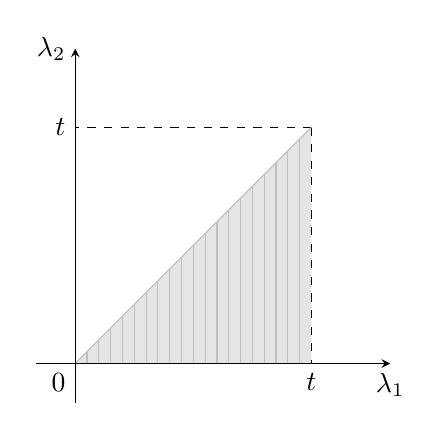
\begin{tikzpicture}
\draw (0,0) node[below left] {$0$};
\fill[lightergray] (0,0)--(3,0)--(3,3);
\draw[dashed] (3,3)--(3,0) node[below] {$t$};
\draw[dashed] (3,3)--(0,3) node[left] {$t$};
\foreach \i in {1,...,19} {
\draw[lightgray] (0.15*\i,0)--(0.15*\i,0.15*\i);
};
\draw[lightgray] (0,0)--(3,3);
\draw[->] (-0.5,0)--(4,0) node[below] {$\lambda_1$};
\draw[->] (0,-0.5)--(0,4) node[left] {$\lambda_2$};
%\foreach \i in {1,...,19} {\draw[lightgray] (0.5*\i,0)--(10,0.5*\i)--(20-0.5*\i,0)--(10,-0.5*\i)--cycle;};
\end{tikzpicture}
\end{center}
and if the integrand $f(\lambda_1,\lambda_2)$ is invariant under the exchange $\lambda_1\leftrightarrow \lambda_2$, we have 
\bse
\int_0^t \d \lambda_1\int_0^{\lambda_1} \d \lambda_2\, f(\lambda_1,\lambda_2) = \frac{1}{2}\int_0^t \d \lambda_1\int_0^t \d \lambda_2\, f(\lambda_1,\lambda_2).
\ese
Generalising to $n$ dimensions, we have
\bse
\int_0^t \d \lambda_1\,\cdots\int_0^{\lambda_{n-1}} \d \lambda_n\, f(\lambda_1,\ldots,\lambda_n) = \frac{1}{n!}\int_0^t \d \lambda_1\,\cdots\int_0^t \d \lambda_n\, f(\lambda_1,\ldots,\lambda_n)
\ese
if $f$ is invariant under any permutation of its arguments. Moreover, since each term in our integrands only depends on one integration variable at a time, we can use
\bse
\int_0^t \d \lambda_1\,\cdots\int_0^{t} \d \lambda_n\, f_1(\lambda_1)\cdots f_n(\lambda_n) = \biggl(\int_0^t \d \lambda_1\,f(\lambda_1)\biggr)\cdots\biggl(\int_0^t \d \lambda_n\, f(\lambda_n)\biggr)
\ese
so that, in our case, we would have
\bi{rCl}
g(t) & = & \biggl(\,\sum_{n=0}^\infty \frac{(-1)^n}{n!}\biggl(\int_0^t \d \lambda  \, \Gamma_\mu(\gamma(\lambda))\dot{\gamma}^\mu(\lambda)\biggr)^{\negmedspace n\,} \biggr)g_0\\
& = & \exp\biggl(-\int_0^t \d \lambda  \, \Gamma_\mu(\gamma(\lambda))\dot{\gamma}^\mu(\lambda)\biggr) g_0.
\ei
However, our integrands are Lie-algebra-valued (that is, matrix valued), and since the factors therein need not commute, they are not invariant under permutations of the independent variables. Hence, the above formula doesn't work. Instead, we write
\bse
g(t)= \mathrm{P}\exp\biggl(-\int_0^t \d \lambda  \, \Gamma_\mu(\gamma(\lambda))\dot{\gamma}^\mu(\lambda)\biggr) g_0,
\ese
where the \emph{path-ordered exponential}\index{path-ordered exponential} $\mathrm{P}\exp$ is defined to yield the correct expression for $g(t)$.

Summarising, we have the following.
\bp
For a principal $G$-bundle $(P,\pi,M)$, where $G$ is a matrix Lie group, the horizontal lift of a curve $\gamma\cl [0,1]\to U$ through $p_p\in \preim_\pi(\{U\})$, where $(U,x)$ is a chart on $M$, is given in terms of a local section $\sigma\cl U \to P$ by the explicit expression
\bse
\gamma^\uparrow(\lambda) = (\sigma\circ\gamma)(\lambda)\racts\biggl(\mathrm{P}\exp\biggl(-\int_0^\lambda \d \widetilde\lambda  \, \Gamma_\mu(\gamma(\widetilde\lambda))\dot{\gamma}^\mu(\widetilde\lambda)\biggr) g_0\biggr).
\ese
\ep

\bd
Let $\gamma^\uparrow_p\cl[0,1]\to P$ be the horizontal lift through $p\in\preim_\pi(\{\gamma(0)\})$ of the curve $\gamma\cl[0,1]\to M$ . The \emph{parallel transport map along $\gamma$}\index{parallel transport map} is the map
\bi{rrCl}
T_\gamma \cl & \preim_\pi(\{\gamma(0)\}) & \to & \preim_\pi(\{\gamma(1)\}) \\
& p & \mapsto & \gamma^\uparrow_p(1).
\ei
\ed
\br
The parallel transport is, in fact, a bijection between the fibres $\preim_\pi(\{\gamma(0)\})$  and $\preim_\pi(\{\gamma(1)\})$. It is injective since there is a unique horizontal lift of $\gamma$ through each point $p\in\preim_\pi(\{\gamma(0)\})$, and horizontal lifts through different points do not intersect.  It is surjective since for each $q\in \preim_\pi(\{\gamma(1)\})$ we can find a $p$ such that $q=\gamma^\uparrow_p(1)$ as follows. Let $\widetilde p\in\preim_\pi(\{\gamma(0)\})$. Then $\gamma^\uparrow_{\widetilde p}(1)$ belongs to the same fibre as $q$ and hence there exists a unique $g\in G$ such that $q = \gamma^\uparrow_{\widetilde p}(1) \racts g$. Recall that 
\bse
\gamma^\uparrow_{\widetilde p}(\lambda) = (\sigma\circ\gamma)(\lambda)\racts (\mathrm{P}\exp (\cdots ) g_0)
\ese
where $g_0$ is the unique $g_0\in G$ such that $\widetilde p = (\sigma\circ\gamma)(0)\racts g_0$. Define $p\in\preim_\pi(\{\gamma(0)\})$ by
\bse
p:=\widetilde p \racts g = (\sigma\circ\gamma)(0)\racts (g_0\bullet g).
\ese
Then we have
\bi{rCl}
\gamma^\uparrow_{p}(1) & = & (\sigma\circ\gamma)(1)\racts (\mathrm{P}\exp (\cdots ) g_0\bullet g)\\
& = & (\sigma\circ\gamma)(1)\racts (\mathrm{P}\exp (\cdots ) g_0)\racts g\\
& = & \gamma^\uparrow_{\widetilde p}(1) \racts g\\
& = & q.
\ei
\er

\subsubsection*{Loops and holonomy groups}
Consider the case of loops, i.e.\ curves $\gamma\cl[0,1]\to M$ for which $\gamma(0)=\gamma(1)$. Fix some $p\in \preim_\pi(\{\gamma(0)\})$. The condition that $\pi\circ\gamma_p^\uparrow=\gamma$ then implies that $\gamma_p^\uparrow(0)$ and $\gamma_p^\uparrow(1)$ belong to the same fibre. Hence, there exists a unique $g_\gamma\in G$ such that
\bse
\gamma_p^\uparrow(1) = \gamma_p^\uparrow(0) \racts g_\gamma=p\racts g_\gamma.
\ese
\bd
Let $\omega$ be a connection one-form on the principal $G$-bundle $(P,\pi,M)$. Let $\gamma\cl[0,1]\to M$ be a loop with base-point $a\in M$, i.e.\ $\gamma(0)=\gamma(1)=a$. The subgroup of $G$
\bse
\Hol_a(\omega) := \{g_\gamma \mid \gamma_p^\uparrow(1) =p\racts g_\gamma \text{ for some loop $\gamma$}\}
\ese
is called the \emph{holonomy group}\index{holonomy group} of $\omega$ on $P$ at the base-point $a$.
\ed

\subsection{Horizontal lifts to the associated bundle}

Almost everything that we have done so far transfers with ease to an associated bundle via the following definition.

\bd
Let $(P,\pi,M)$ be a principal $G$-bundle and $\omega$ a connection one-form on $P$. Let $(P_F,\pi_F,M)$ be an associated fibre bundle of $P$ on whose typical fibre $F$ the Lie group $G$ acts on the left by $\lacts$. Let $\gamma\cl [0,1]\to M$ be a curve on $M$ and let $\gamma^\uparrow_p$ be its horizontal lift to $P$ through $p\in \preim_\pi(\{\gamma(0)\})$. Then the \emph{horizontal lift} of $\gamma$ to the associated bundle $P_F$ through the point $[p,f]\in P_F$ is the curve
\bi{rrCl}
\gamma^{\negmedspace \stackrel{P_F}{\uparrow}}_{[p,f]} \cl & [0,1] & \to & P_F\\
& \lambda & \mapsto & [\gamma^\uparrow_p(\lambda),f]
\ei
\ed
For instance, we have the obvious parallel transport map.
\bd
The \emph{parallel transport map} on the associated bundle is given by
\bi{rrCl}
T^{P_F}_\gamma \cl & \preim_{\pi_F}(\{\gamma(0)\}) & \to & \preim_{\pi_F}(\{\gamma(1)\}) \\
& [p,f] & \mapsto & \gamma^{\negmedspace\stackrel{P_F}{\uparrow}}_{[p,f]}(1).
\ei
\ed

\br
If $F$ is a vector space and $\lacts \cl G\times F \to F$ is fibre-wise linear, i.e.\ for each fixed $g\in G$, the map $(g\lacts -)\cl F \to F$ is linear, then $(P_F,\pi_F,M)$ is called a \emph{vector bundle}. The basic idea of a covariant derivative is as follows. Let $\sigma\cl U \to P_F$ be a local section of the associated bundle. We would like to define the derivative of $\sigma$ at the point $m\in U\se M$ in the direction $X\in T_mM$. By definition, there exists a curve $\gamma\cl(-\varepsilon,\varepsilon)\to M$ with $\gamma(0)=m$ such that $X=X_{\gamma,m}$. Then for any $0\leq t <\varepsilon$, the points $\gamma^{\negmedspace\stackrel{P_F}{\uparrow}}_{[\sigma(m),f]}(t)$ and $\sigma(\gamma(t))$ lie in the same fibre of $P_F$. But since the fibres are vector spaces, we can write the differential quotient
\bse
\frac{\sigma(\gamma(t))-\gamma^{\negmedspace\stackrel{P_F}{\uparrow}}_{[\sigma(m),f]}(t)}{t},
\ese
where the minus sign denotes the additive inverse in the vector space $\preim_{\pi_F}(\{\gamma(t)\})$ and hence define the derivative of $\sigma$ at the point $m$ in the direction $X$, or the derivative of $\sigma$ along $\gamma$ at $\gamma(0)=m$, by 
\bse
\lim_{t\to 0} \frac{\sigma(\gamma(t))-\gamma^{\negmedspace\stackrel{P_F}{\uparrow}}_{[\sigma(m),f]}(t)}{t}.
\ese
\er

















\newpage


% \section{Curvature and torsion on principal bundles}



% \section{Covariant derivatives}



% \section{Application: Quantum mechanics on curved spaces}



% \section{Application: Spin structures}



% \section{Application: Kinematical and dynamical symmetries}

% \newpage

% \section*{Further readings}
% \addcontentsline{toc}{section}{Further readings}
% 
There are several books covering some, most, all, or much more of the course material.

\begin{itemize}
\item Baez, Muniain, \textit{Gauge Fields, Knots and Gravity}, World Scientific 1994
\item Choquet-Bruhat, DeWitt-Morette, \textit{Analysis, manifolds, and physics, Part I: Basics (Revised edition)}, North-Holland 1982
\item Choquet-Bruhat, DeWitt-Morette, \textit{Analysis, manifolds, and physics, Part II (Revised and enlarged edition)}, North-Holland 2000
\item Fecko, \textit{Differential geometry and Lie groups for physicists}, Cambridge University Press 2006
\item Frankel, \textit{The Geometry of Physics: An Introduction} (Third edition),  Cambridge University Press 2011
\item Hamilton, \textit{Mathematical Gauge Theory: With Applications to the Standard Model of Particle Physics}, Springer 2017\\
(preliminary version \url{http://www.mathematik.uni-muenchen.de/~hamilton/gaugetheory.php})
\item Hassani, \textit{Mathematical Physics: A Modern Introduction to Its Foundations (Second edition)}, Springer 2013
\item Lam, \textit{Topics in Contemporary Mathematical Physics (Second edition)}, World Scientific 2015
\item Naber, \textit{Topology, Geometry and Gauge Fields: Foundations (Second edition)}, Springer 2010
\item Nakahara, \textit{Geometry, Topology and Physics (Second edition)}, Institute of Physics Publishing 2003
\item Rudolph, Schmidt, \textit{Differential Geometry and Mathematical Physics: Part I. Manifolds, Lie Groups and Hamiltonian Systems}, Springer 2012
\item Rudolph, Schmidt, \textit{Differential Geometry and Mathematical Physics: Part II. Fibre Bundles, Topology and Gauge Fields}, Springer 2017
\item Schutz, \textit{Geometrical Methods of Mathematical Physics}, Cambridge University Press 1980
\item Szekeres, \textit{A Course in Modern Mathematical Physics: Groups, Hilbert Space and Differential Geometry}, Cambridge University Press 2004
\item Westenholz, \textit{Differential Forms in Mathematical Physics} (Revised edition), North Holland 1978 
\end{itemize}

\noindent Topic-specific references follow.

\subsection*{Logic}

\begin{itemize}
\item Chiswell, Wilfrid, \textit{Mathematical Logic}, Oxford University Press 2007
\item Hammack, \textit{Book of Proof}, Virginia Commonwealth University\\
\url{http://www.people.vcu.edu/~rhammack/BookOfProof/}
\item Mendelson, \textit{Introduction to Mathematical Logic}, CRC Press 2015
\end{itemize}

\subsection*{Set theory}

\begin{itemize}
\item Adamson, \textit{A Set Theory Workbook}, Birkh\"auser 1997
\item Smullyan, Fitting, \textit{Set theory and the continuum problem}, Oxford University Press 1996
\item Takeuti, Zaring, \textit{Introduction to Axiomatic Set Theory}, Springer 1981
\end{itemize}

\subsection*{Topology}

\begin{itemize}
\item Adamson, \textit{A General Topology Workbook}, Birkh\"auser 1995
\item Kalajdzievski, \textit{An Illustrated Introduction to Topology and Homotopy}, CRC Press 2015
\item Munkres, \textit{Topology} (Second edition), Pearson 2014
\end{itemize}

\subsection*{Topological manifolds}

\begin{itemize}
\item Lee, \textit{Introduction to Topological Manifolds} (Second edition), Springer 2011
\end{itemize}

\subsection*{Linear algebra}

\begin{itemize}
\item J\"anich, \textit{Linear algebra}, Springer 1994
\item Lang, \textit{Linear Algebra} (Third edition), Springer 1987
\item Shakarchi, \textit{Solutions Manual for Lang's Linear Algebra}, Springer 1996
\end{itemize}

\subsection*{Differentiable manifolds}

\begin{itemize}
\item Gadea, Masqu\'e, Mykytyuk, \textit{Analysis and Algebra on Differentiable Manifolds: A Workbook for Students and Teachers (Second Edition)}, Springer 2013
\item J\"anich, \textit{Vector Analysis}, Springer 2001
\item Lang, \textit{Fundamentals of Differential Geometry}, Springer 1999
\item Lee, \textit{Introduction to Smooth Manifolds} (Second edition), Springer 2012
\item Warner, \textit{Foundations of Differentiable Manifolds and Lie Groups}, Springer 1983
\end{itemize}

\subsection*{Lie groups and Lie algebras}

\begin{itemize}
\item Das, Okubo, \textit{Lie Groups and Lie Algebras for Physicists}, World Scientific 2014
\item Erdmann, Wildon, \textit{Introduction to Lie Algebras}, Springer 2006
\item Hall, \textit{Lie Groups, Lie Algebras, and Representations: An Elementary Introduction (Second edition)}, Springer 2015
\item Kirillov, \textit{An Introduction to Lie Groups and Lie Algebras}, Cambridge University Press 2008
\item Stillwell, \textit{Naive Lie Theory}, Springer 2008
\end{itemize}

\subsection*{Representation theory}

\begin{itemize}
\item Fuchs, Schweigert, \textit{Symmetries, Lie Algebras and Representations: A Graduate Course for Physicists}, Cambridge University Press 1997
\item Fulton, Harris, \textit{Representation Theory: A First Course}, Springer 2004
\item Zee, \textit{Group Theory in a Nutshell for Physicists}, Princeton University Press 2016
\end{itemize}

\subsection*{Principal bundles}

\begin{itemize}
\item Sontz, \textit{Principal Bundles: The Classical Case}, Springer 2015
\item Sontz, \textit{Principal Bundles: The Quantum Case}, Springer 2015
\end{itemize}











% \printindex

\end{document}
